\documentclass[twoside]{book}

% Packages required by doxygen
\usepackage{fixltx2e}
\usepackage{calc}
\usepackage{doxygen}
\usepackage[export]{adjustbox} % also loads graphicx
\usepackage{graphicx}
\usepackage[utf8]{inputenc}
\usepackage{makeidx}
\usepackage{multicol}
\usepackage{multirow}
\PassOptionsToPackage{warn}{textcomp}
\usepackage{textcomp}
\usepackage[nointegrals]{wasysym}
\usepackage[table]{xcolor}

% Font selection
\usepackage[T1]{fontenc}
\usepackage[scaled=.90]{helvet}
\usepackage{courier}
\usepackage{amssymb}
\usepackage{sectsty}
\renewcommand{\familydefault}{\sfdefault}
\allsectionsfont{%
  \fontseries{bc}\selectfont%
  \color{darkgray}%
}
\renewcommand{\DoxyLabelFont}{%
  \fontseries{bc}\selectfont%
  \color{darkgray}%
}
\newcommand{\+}{\discretionary{\mbox{\scriptsize$\hookleftarrow$}}{}{}}

% Page & text layout
\usepackage{geometry}
\geometry{%
  a4paper,%
  top=2.5cm,%
  bottom=2.5cm,%
  left=2.5cm,%
  right=2.5cm%
}
\tolerance=750
\hfuzz=15pt
\hbadness=750
\setlength{\emergencystretch}{15pt}
\setlength{\parindent}{0cm}
\setlength{\parskip}{3ex plus 2ex minus 2ex}
\makeatletter
\renewcommand{\paragraph}{%
  \@startsection{paragraph}{4}{0ex}{-1.0ex}{1.0ex}{%
    \normalfont\normalsize\bfseries\SS@parafont%
  }%
}
\renewcommand{\subparagraph}{%
  \@startsection{subparagraph}{5}{0ex}{-1.0ex}{1.0ex}{%
    \normalfont\normalsize\bfseries\SS@subparafont%
  }%
}
\makeatother

% Headers & footers
\usepackage{fancyhdr}
\pagestyle{fancyplain}
\fancyhead[LE]{\fancyplain{}{\bfseries\thepage}}
\fancyhead[CE]{\fancyplain{}{}}
\fancyhead[RE]{\fancyplain{}{\bfseries\leftmark}}
\fancyhead[LO]{\fancyplain{}{\bfseries\rightmark}}
\fancyhead[CO]{\fancyplain{}{}}
\fancyhead[RO]{\fancyplain{}{\bfseries\thepage}}
\fancyfoot[LE]{\fancyplain{}{}}
\fancyfoot[CE]{\fancyplain{}{}}
\fancyfoot[RE]{\fancyplain{}{\bfseries\scriptsize Generated by Doxygen }}
\fancyfoot[LO]{\fancyplain{}{\bfseries\scriptsize Generated by Doxygen }}
\fancyfoot[CO]{\fancyplain{}{}}
\fancyfoot[RO]{\fancyplain{}{}}
\renewcommand{\footrulewidth}{0.4pt}
\renewcommand{\chaptermark}[1]{%
  \markboth{#1}{}%
}
\renewcommand{\sectionmark}[1]{%
  \markright{\thesection\ #1}%
}

% Indices & bibliography
\usepackage{natbib}
\usepackage[titles]{tocloft}
\setcounter{tocdepth}{3}
\setcounter{secnumdepth}{5}
\makeindex

% Hyperlinks (required, but should be loaded last)
\usepackage{ifpdf}
\ifpdf
  \usepackage[pdftex,pagebackref=true]{hyperref}
\else
  \usepackage[ps2pdf,pagebackref=true]{hyperref}
\fi
\hypersetup{%
  colorlinks=true,%
  linkcolor=blue,%
  citecolor=blue,%
  unicode%
}

% Custom commands
\newcommand{\clearemptydoublepage}{%
  \newpage{\pagestyle{empty}\cleardoublepage}%
}

\usepackage{caption}
\captionsetup{labelsep=space,justification=centering,font={bf},singlelinecheck=off,skip=4pt,position=top}

%===== C O N T E N T S =====

\begin{document}

% Titlepage & ToC
\hypersetup{pageanchor=false,
             bookmarksnumbered=true,
             pdfencoding=unicode
            }
\pagenumbering{alph}
\begin{titlepage}
\vspace*{7cm}
\begin{center}%
{\Large \mbox{[}O\+L\+C2\mbox{]}P1\+\_\+201504242 }\\
\vspace*{1cm}
{\large Generated by Doxygen 1.8.14}\\
\end{center}
\end{titlepage}
\clearemptydoublepage
\pagenumbering{roman}
\tableofcontents
\clearemptydoublepage
\pagenumbering{arabic}
\hypersetup{pageanchor=true}

%--- Begin generated contents ---
\chapter{Deprecated List}
\label{deprecated}
\Hypertarget{deprecated}

\begin{DoxyRefList}
\item[\label{deprecated__deprecated000001}%
\Hypertarget{deprecated__deprecated000001}%
Member \mbox{\hyperlink{classanalizadores_1_1_simple_char_stream_ad9fd1239a7ecd61c0106e6863d8f81cd}{analizadores.Simple\+Char\+Stream.get\+Column}} ()]
\item[\label{deprecated__deprecated000002}%
\Hypertarget{deprecated__deprecated000002}%
Member \mbox{\hyperlink{classanalizadores_1_1_simple_char_stream_ad2af5c3f4fadce0ec36b08eb5bc67b42}{analizadores.Simple\+Char\+Stream.get\+Line}} ()]
\end{DoxyRefList}
\chapter{Namespace Index}
\section{Packages}
Here are the packages with brief descriptions (if available)\+:\begin{DoxyCompactList}
\item\contentsline{section}{\mbox{\hyperlink{namespaceanalizadores}{analizadores}} }{\pageref{namespaceanalizadores}}{}
\end{DoxyCompactList}

\chapter{Hierarchical Index}
\section{Class Hierarchy}
This inheritance list is sorted roughly, but not completely, alphabetically\+:\begin{DoxyCompactList}
\item \contentsline{section}{entorno.\+Simbolo.\+Acc}{\pageref{enumentorno_1_1_simbolo_1_1_acc}}{}
\item \contentsline{section}{ast.\+A\+ST}{\pageref{classast_1_1_a_s_t}}{}
\item \contentsline{section}{ast.\+instrucciones.\+Condicion}{\pageref{classast_1_1instrucciones_1_1_condicion}}{}
\begin{DoxyCompactList}
\item \contentsline{section}{ast.\+instrucciones.\+Do\+While}{\pageref{classast_1_1instrucciones_1_1_do_while}}{}
\item \contentsline{section}{ast.\+instrucciones.\+For}{\pageref{classast_1_1instrucciones_1_1_for}}{}
\item \contentsline{section}{ast.\+instrucciones.\+If}{\pageref{classast_1_1instrucciones_1_1_if}}{}
\item \contentsline{section}{ast.\+instrucciones.\+While}{\pageref{classast_1_1instrucciones_1_1_while}}{}
\end{DoxyCompactList}
\item \contentsline{section}{entorno.\+Entorno}{\pageref{classentorno_1_1_entorno}}{}
\item Error\begin{DoxyCompactList}
\item \contentsline{section}{analizadores.\+Token\+Mgr\+Error}{\pageref{classanalizadores_1_1_token_mgr_error}}{}
\end{DoxyCompactList}
\item Exception\begin{DoxyCompactList}
\item \contentsline{section}{analizadores.\+Parse\+Exception}{\pageref{classanalizadores_1_1_parse_exception}}{}
\end{DoxyCompactList}
\item \contentsline{section}{analizadores.\+Gramatica\+Constants}{\pageref{interfaceanalizadores_1_1_gramatica_constants}}{}
\begin{DoxyCompactList}
\item \contentsline{section}{analizadores.\+Gramatica}{\pageref{classanalizadores_1_1_gramatica}}{}
\item \contentsline{section}{analizadores.\+Gramatica\+Token\+Manager}{\pageref{classanalizadores_1_1_gramatica_token_manager}}{}
\end{DoxyCompactList}
\item \contentsline{section}{olc2.\+p1\+\_\+201504242.\+J\+Error}{\pageref{classolc2_1_1p1__201504242_1_1_j_error}}{}
\item J\+Frame\begin{DoxyCompactList}
\item \contentsline{section}{olc2.\+p1\+\_\+201504242.\+Ventana}{\pageref{classolc2_1_1p1__201504242_1_1_ventana}}{}
\end{DoxyCompactList}
\item lr\+\_\+parser\begin{DoxyCompactList}
\item \contentsline{section}{analizadores.\+Sintactico}{\pageref{classanalizadores_1_1_sintactico}}{}
\end{DoxyCompactList}
\item \contentsline{section}{J\+Lex.\+Main}{\pageref{class_j_lex_1_1_main}}{}
\item \contentsline{section}{ast.\+instrucciones.\+funciones.\+Modificador\+Matrix}{\pageref{classast_1_1instrucciones_1_1funciones_1_1_modificador_matrix}}{}
\item \contentsline{section}{ast.\+Nodo\+A\+ST}{\pageref{interfaceast_1_1_nodo_a_s_t}}{}
\begin{DoxyCompactList}
\item \contentsline{section}{ast.\+Expresion}{\pageref{interfaceast_1_1_expresion}}{}
\begin{DoxyCompactList}
\item \contentsline{section}{ast.\+expresiones.\+Identificador}{\pageref{classast_1_1expresiones_1_1_identificador}}{}
\item \contentsline{section}{ast.\+expresiones.\+Literal}{\pageref{classast_1_1expresiones_1_1_literal}}{}
\item \contentsline{section}{ast.\+expresiones.\+Llama}{\pageref{classast_1_1expresiones_1_1_llama}}{}
\item \contentsline{section}{ast.\+expresiones.\+operaciones.\+Operacion}{\pageref{classast_1_1expresiones_1_1operaciones_1_1_operacion}}{}
\begin{DoxyCompactList}
\item \contentsline{section}{ast.\+expresiones.\+operaciones.\+Aritmetica}{\pageref{classast_1_1expresiones_1_1operaciones_1_1_aritmetica}}{}
\item \contentsline{section}{ast.\+expresiones.\+operaciones.\+Logica}{\pageref{classast_1_1expresiones_1_1operaciones_1_1_logica}}{}
\item \contentsline{section}{ast.\+expresiones.\+operaciones.\+Relacional}{\pageref{classast_1_1expresiones_1_1operaciones_1_1_relacional}}{}
\end{DoxyCompactList}
\item \contentsline{section}{ast.\+expresiones.\+operaciones.\+Ternaria}{\pageref{classast_1_1expresiones_1_1operaciones_1_1_ternaria}}{}
\item \contentsline{section}{ast.\+expresiones.\+Return}{\pageref{classast_1_1expresiones_1_1_return}}{}
\item \contentsline{section}{ast.\+instrucciones.\+funciones.\+Fnum}{\pageref{classast_1_1instrucciones_1_1funciones_1_1_fnum}}{}
\item \contentsline{section}{ast.\+instrucciones.\+funciones.\+Fstring}{\pageref{classast_1_1instrucciones_1_1funciones_1_1_fstring}}{}
\item \contentsline{section}{ast.\+instrucciones.\+funciones.\+funcionC}{\pageref{classast_1_1instrucciones_1_1funciones_1_1funcion_c}}{}
\item \contentsline{section}{ast.\+instrucciones.\+funciones.\+Funcion\+Matrix}{\pageref{classast_1_1instrucciones_1_1funciones_1_1_funcion_matrix}}{}
\item \contentsline{section}{ast.\+instrucciones.\+funciones.\+Generar\+List}{\pageref{classast_1_1instrucciones_1_1funciones_1_1_generar_list}}{}
\item \contentsline{section}{ast.\+instrucciones.\+funciones.\+Length}{\pageref{classast_1_1instrucciones_1_1funciones_1_1_length}}{}
\item \contentsline{section}{ast.\+instrucciones.\+funciones.\+n\+Matrix}{\pageref{classast_1_1instrucciones_1_1funciones_1_1n_matrix}}{}
\item \contentsline{section}{ast.\+instrucciones.\+funciones.\+Typeof}{\pageref{classast_1_1instrucciones_1_1funciones_1_1_typeof}}{}
\end{DoxyCompactList}
\item \contentsline{section}{ast.\+Instruccion}{\pageref{interfaceast_1_1_instruccion}}{}
\begin{DoxyCompactList}
\item \contentsline{section}{ast.\+instrucciones.\+Asignacion}{\pageref{classast_1_1instrucciones_1_1_asignacion}}{}
\item \contentsline{section}{ast.\+instrucciones.\+Break}{\pageref{classast_1_1instrucciones_1_1_break}}{}
\item \contentsline{section}{ast.\+instrucciones.\+Continue}{\pageref{classast_1_1instrucciones_1_1_continue}}{}
\item \contentsline{section}{ast.\+instrucciones.\+Do\+While}{\pageref{classast_1_1instrucciones_1_1_do_while}}{}
\item \contentsline{section}{ast.\+instrucciones.\+For}{\pageref{classast_1_1instrucciones_1_1_for}}{}
\item \contentsline{section}{ast.\+instrucciones.\+Funcion}{\pageref{classast_1_1instrucciones_1_1_funcion}}{}
\item \contentsline{section}{ast.\+instrucciones.\+funciones.\+Print}{\pageref{classast_1_1instrucciones_1_1funciones_1_1_print}}{}
\item \contentsline{section}{ast.\+instrucciones.\+graficas.\+graf\+Barras}{\pageref{classast_1_1instrucciones_1_1graficas_1_1graf_barras}}{}
\item \contentsline{section}{ast.\+instrucciones.\+graficas.\+graf\+Dispersion}{\pageref{classast_1_1instrucciones_1_1graficas_1_1graf_dispersion}}{}
\item \contentsline{section}{ast.\+instrucciones.\+graficas.\+graf\+Histograma}{\pageref{classast_1_1instrucciones_1_1graficas_1_1graf_histograma}}{}
\item \contentsline{section}{ast.\+instrucciones.\+graficas.\+graf\+Lineas}{\pageref{classast_1_1instrucciones_1_1graficas_1_1graf_lineas}}{}
\item \contentsline{section}{ast.\+instrucciones.\+graficas.\+graf\+Pie}{\pageref{classast_1_1instrucciones_1_1graficas_1_1graf_pie}}{}
\item \contentsline{section}{ast.\+instrucciones.\+If}{\pageref{classast_1_1instrucciones_1_1_if}}{}
\item \contentsline{section}{ast.\+instrucciones.\+While}{\pageref{classast_1_1instrucciones_1_1_while}}{}
\item \contentsline{section}{entorno.\+fantasmita}{\pageref{classentorno_1_1fantasmita}}{}
\end{DoxyCompactList}
\end{DoxyCompactList}
\item \contentsline{section}{entorno.\+nodo\+Exp}{\pageref{classentorno_1_1nodo_exp}}{}
\item \contentsline{section}{olc2.\+p1\+\_\+201504242.\+O\+L\+C2\+P1\+\_\+201504242}{\pageref{classolc2_1_1p1__201504242_1_1_o_l_c2_p1__201504242}}{}
\item \contentsline{section}{ast.\+expresiones.\+operaciones.\+Operacion.\+Operador}{\pageref{enumast_1_1expresiones_1_1operaciones_1_1_operacion_1_1_operador}}{}
\item \contentsline{section}{entorno.\+Simbolo.\+Rol}{\pageref{enumentorno_1_1_simbolo_1_1_rol}}{}
\item Scanner\begin{DoxyCompactList}
\item \contentsline{section}{analizadores.\+Lexico}{\pageref{classanalizadores_1_1_lexico}}{}
\end{DoxyCompactList}
\item \contentsline{section}{entorno.\+Simbolo}{\pageref{classentorno_1_1_simbolo}}{}
\begin{DoxyCompactList}
\item \contentsline{section}{ast.\+instrucciones.\+Funcion}{\pageref{classast_1_1instrucciones_1_1_funcion}}{}
\end{DoxyCompactList}
\item \contentsline{section}{analizadores.\+Simple\+Char\+Stream}{\pageref{classanalizadores_1_1_simple_char_stream}}{}
\item \contentsline{section}{analizadores.\+sym}{\pageref{classanalizadores_1_1sym}}{}
\item \contentsline{section}{entorno.\+Tipo}{\pageref{classentorno_1_1_tipo}}{}
\item \contentsline{section}{entorno.\+Tipo.\+Tipos}{\pageref{enumentorno_1_1_tipo_1_1_tipos}}{}
\item \contentsline{section}{analizadores.\+Token}{\pageref{classanalizadores_1_1_token}}{}
\item \contentsline{section}{entorno.\+Var}{\pageref{classentorno_1_1_var}}{}
\item Linked\+List\begin{DoxyCompactList}
\item \contentsline{section}{ast.\+instrucciones.\+funciones.\+List\+Var}{\pageref{classast_1_1instrucciones_1_1funciones_1_1_list_var}}{}
\end{DoxyCompactList}
\item R\+Text\+Scroll\+Pane\begin{DoxyCompactList}
\item \contentsline{section}{olc2.\+p1\+\_\+201504242.\+Editor}{\pageref{classolc2_1_1p1__201504242_1_1_editor}}{}
\end{DoxyCompactList}
\end{DoxyCompactList}

\chapter{Class Index}
\section{Class List}
Here are the classes, structs, unions and interfaces with brief descriptions\+:\begin{DoxyCompactList}
\item\contentsline{section}{\mbox{\hyperlink{enumentorno_1_1_simbolo_1_1_acc}{entorno.\+Simbolo.\+Acc}} }{\pageref{enumentorno_1_1_simbolo_1_1_acc}}{}
\item\contentsline{section}{\mbox{\hyperlink{classast_1_1expresiones_1_1operaciones_1_1_aritmetica}{ast.\+expresiones.\+operaciones.\+Aritmetica}} }{\pageref{classast_1_1expresiones_1_1operaciones_1_1_aritmetica}}{}
\item\contentsline{section}{\mbox{\hyperlink{classast_1_1instrucciones_1_1_asignacion}{ast.\+instrucciones.\+Asignacion}} }{\pageref{classast_1_1instrucciones_1_1_asignacion}}{}
\item\contentsline{section}{\mbox{\hyperlink{classast_1_1_a_s_t}{ast.\+A\+ST}} }{\pageref{classast_1_1_a_s_t}}{}
\item\contentsline{section}{\mbox{\hyperlink{classast_1_1instrucciones_1_1_break}{ast.\+instrucciones.\+Break}} }{\pageref{classast_1_1instrucciones_1_1_break}}{}
\item\contentsline{section}{\mbox{\hyperlink{classast_1_1instrucciones_1_1_condicion}{ast.\+instrucciones.\+Condicion}} }{\pageref{classast_1_1instrucciones_1_1_condicion}}{}
\item\contentsline{section}{\mbox{\hyperlink{classast_1_1instrucciones_1_1_continue}{ast.\+instrucciones.\+Continue}} }{\pageref{classast_1_1instrucciones_1_1_continue}}{}
\item\contentsline{section}{\mbox{\hyperlink{classast_1_1instrucciones_1_1_do_while}{ast.\+instrucciones.\+Do\+While}} }{\pageref{classast_1_1instrucciones_1_1_do_while}}{}
\item\contentsline{section}{\mbox{\hyperlink{classolc2_1_1p1__201504242_1_1_editor}{olc2.\+p1\+\_\+201504242.\+Editor}} }{\pageref{classolc2_1_1p1__201504242_1_1_editor}}{}
\item\contentsline{section}{\mbox{\hyperlink{classentorno_1_1_entorno}{entorno.\+Entorno}} }{\pageref{classentorno_1_1_entorno}}{}
\item\contentsline{section}{\mbox{\hyperlink{interfaceast_1_1_expresion}{ast.\+Expresion}} }{\pageref{interfaceast_1_1_expresion}}{}
\item\contentsline{section}{\mbox{\hyperlink{classentorno_1_1fantasmita}{entorno.\+fantasmita}} }{\pageref{classentorno_1_1fantasmita}}{}
\item\contentsline{section}{\mbox{\hyperlink{classast_1_1instrucciones_1_1funciones_1_1_fnum}{ast.\+instrucciones.\+funciones.\+Fnum}} }{\pageref{classast_1_1instrucciones_1_1funciones_1_1_fnum}}{}
\item\contentsline{section}{\mbox{\hyperlink{classast_1_1instrucciones_1_1_for}{ast.\+instrucciones.\+For}} }{\pageref{classast_1_1instrucciones_1_1_for}}{}
\item\contentsline{section}{\mbox{\hyperlink{classast_1_1instrucciones_1_1funciones_1_1_fstring}{ast.\+instrucciones.\+funciones.\+Fstring}} }{\pageref{classast_1_1instrucciones_1_1funciones_1_1_fstring}}{}
\item\contentsline{section}{\mbox{\hyperlink{classast_1_1instrucciones_1_1_funcion}{ast.\+instrucciones.\+Funcion}} }{\pageref{classast_1_1instrucciones_1_1_funcion}}{}
\item\contentsline{section}{\mbox{\hyperlink{classast_1_1instrucciones_1_1funciones_1_1funcion_c}{ast.\+instrucciones.\+funciones.\+funcionC}} }{\pageref{classast_1_1instrucciones_1_1funciones_1_1funcion_c}}{}
\item\contentsline{section}{\mbox{\hyperlink{classast_1_1instrucciones_1_1funciones_1_1_funcion_matrix}{ast.\+instrucciones.\+funciones.\+Funcion\+Matrix}} }{\pageref{classast_1_1instrucciones_1_1funciones_1_1_funcion_matrix}}{}
\item\contentsline{section}{\mbox{\hyperlink{classast_1_1instrucciones_1_1funciones_1_1_generar_list}{ast.\+instrucciones.\+funciones.\+Generar\+List}} }{\pageref{classast_1_1instrucciones_1_1funciones_1_1_generar_list}}{}
\item\contentsline{section}{\mbox{\hyperlink{classast_1_1instrucciones_1_1graficas_1_1graf_barras}{ast.\+instrucciones.\+graficas.\+graf\+Barras}} }{\pageref{classast_1_1instrucciones_1_1graficas_1_1graf_barras}}{}
\item\contentsline{section}{\mbox{\hyperlink{classast_1_1instrucciones_1_1graficas_1_1graf_dispersion}{ast.\+instrucciones.\+graficas.\+graf\+Dispersion}} }{\pageref{classast_1_1instrucciones_1_1graficas_1_1graf_dispersion}}{}
\item\contentsline{section}{\mbox{\hyperlink{classast_1_1instrucciones_1_1graficas_1_1graf_histograma}{ast.\+instrucciones.\+graficas.\+graf\+Histograma}} }{\pageref{classast_1_1instrucciones_1_1graficas_1_1graf_histograma}}{}
\item\contentsline{section}{\mbox{\hyperlink{classast_1_1instrucciones_1_1graficas_1_1graf_lineas}{ast.\+instrucciones.\+graficas.\+graf\+Lineas}} }{\pageref{classast_1_1instrucciones_1_1graficas_1_1graf_lineas}}{}
\item\contentsline{section}{\mbox{\hyperlink{classast_1_1instrucciones_1_1graficas_1_1graf_pie}{ast.\+instrucciones.\+graficas.\+graf\+Pie}} }{\pageref{classast_1_1instrucciones_1_1graficas_1_1graf_pie}}{}
\item\contentsline{section}{\mbox{\hyperlink{classanalizadores_1_1_gramatica}{analizadores.\+Gramatica}} }{\pageref{classanalizadores_1_1_gramatica}}{}
\item\contentsline{section}{\mbox{\hyperlink{interfaceanalizadores_1_1_gramatica_constants}{analizadores.\+Gramatica\+Constants}} }{\pageref{interfaceanalizadores_1_1_gramatica_constants}}{}
\item\contentsline{section}{\mbox{\hyperlink{classanalizadores_1_1_gramatica_token_manager}{analizadores.\+Gramatica\+Token\+Manager}} }{\pageref{classanalizadores_1_1_gramatica_token_manager}}{}
\item\contentsline{section}{\mbox{\hyperlink{classast_1_1expresiones_1_1_identificador}{ast.\+expresiones.\+Identificador}} }{\pageref{classast_1_1expresiones_1_1_identificador}}{}
\item\contentsline{section}{\mbox{\hyperlink{classast_1_1instrucciones_1_1_if}{ast.\+instrucciones.\+If}} }{\pageref{classast_1_1instrucciones_1_1_if}}{}
\item\contentsline{section}{\mbox{\hyperlink{interfaceast_1_1_instruccion}{ast.\+Instruccion}} }{\pageref{interfaceast_1_1_instruccion}}{}
\item\contentsline{section}{\mbox{\hyperlink{classolc2_1_1p1__201504242_1_1_j_error}{olc2.\+p1\+\_\+201504242.\+J\+Error}} }{\pageref{classolc2_1_1p1__201504242_1_1_j_error}}{}
\item\contentsline{section}{\mbox{\hyperlink{classast_1_1instrucciones_1_1funciones_1_1_length}{ast.\+instrucciones.\+funciones.\+Length}} }{\pageref{classast_1_1instrucciones_1_1funciones_1_1_length}}{}
\item\contentsline{section}{\mbox{\hyperlink{classanalizadores_1_1_lexico}{analizadores.\+Lexico}} }{\pageref{classanalizadores_1_1_lexico}}{}
\item\contentsline{section}{\mbox{\hyperlink{classast_1_1instrucciones_1_1funciones_1_1_list_var}{ast.\+instrucciones.\+funciones.\+List\+Var}} }{\pageref{classast_1_1instrucciones_1_1funciones_1_1_list_var}}{}
\item\contentsline{section}{\mbox{\hyperlink{classast_1_1expresiones_1_1_literal}{ast.\+expresiones.\+Literal}} }{\pageref{classast_1_1expresiones_1_1_literal}}{}
\item\contentsline{section}{\mbox{\hyperlink{classast_1_1expresiones_1_1_llama}{ast.\+expresiones.\+Llama}} }{\pageref{classast_1_1expresiones_1_1_llama}}{}
\item\contentsline{section}{\mbox{\hyperlink{classast_1_1expresiones_1_1operaciones_1_1_logica}{ast.\+expresiones.\+operaciones.\+Logica}} }{\pageref{classast_1_1expresiones_1_1operaciones_1_1_logica}}{}
\item\contentsline{section}{\mbox{\hyperlink{class_j_lex_1_1_main}{J\+Lex.\+Main}} }{\pageref{class_j_lex_1_1_main}}{}
\item\contentsline{section}{\mbox{\hyperlink{classast_1_1instrucciones_1_1funciones_1_1_modificador_matrix}{ast.\+instrucciones.\+funciones.\+Modificador\+Matrix}} }{\pageref{classast_1_1instrucciones_1_1funciones_1_1_modificador_matrix}}{}
\item\contentsline{section}{\mbox{\hyperlink{classast_1_1instrucciones_1_1funciones_1_1n_matrix}{ast.\+instrucciones.\+funciones.\+n\+Matrix}} }{\pageref{classast_1_1instrucciones_1_1funciones_1_1n_matrix}}{}
\item\contentsline{section}{\mbox{\hyperlink{interfaceast_1_1_nodo_a_s_t}{ast.\+Nodo\+A\+ST}} }{\pageref{interfaceast_1_1_nodo_a_s_t}}{}
\item\contentsline{section}{\mbox{\hyperlink{classentorno_1_1nodo_exp}{entorno.\+nodo\+Exp}} }{\pageref{classentorno_1_1nodo_exp}}{}
\item\contentsline{section}{\mbox{\hyperlink{classolc2_1_1p1__201504242_1_1_o_l_c2_p1__201504242}{olc2.\+p1\+\_\+201504242.\+O\+L\+C2\+P1\+\_\+201504242}} }{\pageref{classolc2_1_1p1__201504242_1_1_o_l_c2_p1__201504242}}{}
\item\contentsline{section}{\mbox{\hyperlink{classast_1_1expresiones_1_1operaciones_1_1_operacion}{ast.\+expresiones.\+operaciones.\+Operacion}} }{\pageref{classast_1_1expresiones_1_1operaciones_1_1_operacion}}{}
\item\contentsline{section}{\mbox{\hyperlink{enumast_1_1expresiones_1_1operaciones_1_1_operacion_1_1_operador}{ast.\+expresiones.\+operaciones.\+Operacion.\+Operador}} }{\pageref{enumast_1_1expresiones_1_1operaciones_1_1_operacion_1_1_operador}}{}
\item\contentsline{section}{\mbox{\hyperlink{classanalizadores_1_1_parse_exception}{analizadores.\+Parse\+Exception}} }{\pageref{classanalizadores_1_1_parse_exception}}{}
\item\contentsline{section}{\mbox{\hyperlink{classast_1_1instrucciones_1_1funciones_1_1_print}{ast.\+instrucciones.\+funciones.\+Print}} }{\pageref{classast_1_1instrucciones_1_1funciones_1_1_print}}{}
\item\contentsline{section}{\mbox{\hyperlink{classast_1_1expresiones_1_1operaciones_1_1_relacional}{ast.\+expresiones.\+operaciones.\+Relacional}} }{\pageref{classast_1_1expresiones_1_1operaciones_1_1_relacional}}{}
\item\contentsline{section}{\mbox{\hyperlink{classast_1_1expresiones_1_1_return}{ast.\+expresiones.\+Return}} }{\pageref{classast_1_1expresiones_1_1_return}}{}
\item\contentsline{section}{\mbox{\hyperlink{enumentorno_1_1_simbolo_1_1_rol}{entorno.\+Simbolo.\+Rol}} }{\pageref{enumentorno_1_1_simbolo_1_1_rol}}{}
\item\contentsline{section}{\mbox{\hyperlink{classentorno_1_1_simbolo}{entorno.\+Simbolo}} }{\pageref{classentorno_1_1_simbolo}}{}
\item\contentsline{section}{\mbox{\hyperlink{classanalizadores_1_1_simple_char_stream}{analizadores.\+Simple\+Char\+Stream}} }{\pageref{classanalizadores_1_1_simple_char_stream}}{}
\item\contentsline{section}{\mbox{\hyperlink{classanalizadores_1_1_sintactico}{analizadores.\+Sintactico}} }{\pageref{classanalizadores_1_1_sintactico}}{}
\item\contentsline{section}{\mbox{\hyperlink{classanalizadores_1_1sym}{analizadores.\+sym}} }{\pageref{classanalizadores_1_1sym}}{}
\item\contentsline{section}{\mbox{\hyperlink{classast_1_1expresiones_1_1operaciones_1_1_ternaria}{ast.\+expresiones.\+operaciones.\+Ternaria}} }{\pageref{classast_1_1expresiones_1_1operaciones_1_1_ternaria}}{}
\item\contentsline{section}{\mbox{\hyperlink{classentorno_1_1_tipo}{entorno.\+Tipo}} }{\pageref{classentorno_1_1_tipo}}{}
\item\contentsline{section}{\mbox{\hyperlink{enumentorno_1_1_tipo_1_1_tipos}{entorno.\+Tipo.\+Tipos}} }{\pageref{enumentorno_1_1_tipo_1_1_tipos}}{}
\item\contentsline{section}{\mbox{\hyperlink{classanalizadores_1_1_token}{analizadores.\+Token}} }{\pageref{classanalizadores_1_1_token}}{}
\item\contentsline{section}{\mbox{\hyperlink{classanalizadores_1_1_token_mgr_error}{analizadores.\+Token\+Mgr\+Error}} }{\pageref{classanalizadores_1_1_token_mgr_error}}{}
\item\contentsline{section}{\mbox{\hyperlink{classast_1_1instrucciones_1_1funciones_1_1_typeof}{ast.\+instrucciones.\+funciones.\+Typeof}} }{\pageref{classast_1_1instrucciones_1_1funciones_1_1_typeof}}{}
\item\contentsline{section}{\mbox{\hyperlink{classentorno_1_1_var}{entorno.\+Var}} }{\pageref{classentorno_1_1_var}}{}
\item\contentsline{section}{\mbox{\hyperlink{classolc2_1_1p1__201504242_1_1_ventana}{olc2.\+p1\+\_\+201504242.\+Ventana}} }{\pageref{classolc2_1_1p1__201504242_1_1_ventana}}{}
\item\contentsline{section}{\mbox{\hyperlink{classast_1_1instrucciones_1_1_while}{ast.\+instrucciones.\+While}} }{\pageref{classast_1_1instrucciones_1_1_while}}{}
\end{DoxyCompactList}

\chapter{Namespace Documentation}
\hypertarget{namespaceanalizadores}{}\section{Package analizadores}
\label{namespaceanalizadores}\index{analizadores@{analizadores}}
\subsection*{Classes}
\begin{DoxyCompactItemize}
\item 
class \mbox{\hyperlink{classanalizadores_1_1_gramatica}{Gramatica}}
\item 
interface \mbox{\hyperlink{interfaceanalizadores_1_1_gramatica_constants}{Gramatica\+Constants}}
\item 
class \mbox{\hyperlink{classanalizadores_1_1_gramatica_token_manager}{Gramatica\+Token\+Manager}}
\item 
class \mbox{\hyperlink{classanalizadores_1_1_lexico}{Lexico}}
\item 
class \mbox{\hyperlink{classanalizadores_1_1_parse_exception}{Parse\+Exception}}
\item 
class \mbox{\hyperlink{classanalizadores_1_1_simple_char_stream}{Simple\+Char\+Stream}}
\item 
class \mbox{\hyperlink{classanalizadores_1_1_sintactico}{Sintactico}}
\item 
class \mbox{\hyperlink{classanalizadores_1_1sym}{sym}}
\item 
class \mbox{\hyperlink{classanalizadores_1_1_token}{Token}}
\item 
class \mbox{\hyperlink{classanalizadores_1_1_token_mgr_error}{Token\+Mgr\+Error}}
\end{DoxyCompactItemize}


\subsection{Detailed Description}
Analizador de expresiones aritmeticas sencillas. 
\chapter{Class Documentation}
\hypertarget{enumentorno_1_1_simbolo_1_1_acc}{}\section{entorno.\+Simbolo.\+Acc Enum Reference}
\label{enumentorno_1_1_simbolo_1_1_acc}\index{entorno.\+Simbolo.\+Acc@{entorno.\+Simbolo.\+Acc}}
\subsection*{Public Attributes}
\begin{DoxyCompactItemize}
\item 
\mbox{\Hypertarget{enumentorno_1_1_simbolo_1_1_acc_abd18e4836ad2134f041d80f5800c731a}\label{enumentorno_1_1_simbolo_1_1_acc_abd18e4836ad2134f041d80f5800c731a}} 
{\bfseries tipo1}
\item 
\mbox{\Hypertarget{enumentorno_1_1_simbolo_1_1_acc_ad3532567460535b0b6d89f7a212c4f9f}\label{enumentorno_1_1_simbolo_1_1_acc_ad3532567460535b0b6d89f7a212c4f9f}} 
{\bfseries tipo2}
\item 
\mbox{\Hypertarget{enumentorno_1_1_simbolo_1_1_acc_ac721376d3ffdc144ee08fa43276944c6}\label{enumentorno_1_1_simbolo_1_1_acc_ac721376d3ffdc144ee08fa43276944c6}} 
{\bfseries m1}
\item 
\mbox{\Hypertarget{enumentorno_1_1_simbolo_1_1_acc_a2948282532280e8bcf5ca3f40a4c8e41}\label{enumentorno_1_1_simbolo_1_1_acc_a2948282532280e8bcf5ca3f40a4c8e41}} 
{\bfseries m2}
\item 
\mbox{\Hypertarget{enumentorno_1_1_simbolo_1_1_acc_a9575a901d6073b2e1d394327d996cc7d}\label{enumentorno_1_1_simbolo_1_1_acc_a9575a901d6073b2e1d394327d996cc7d}} 
{\bfseries m3}
\end{DoxyCompactItemize}


The documentation for this enum was generated from the following file\+:\begin{DoxyCompactItemize}
\item 
src/entorno/Simbolo.\+java\end{DoxyCompactItemize}

\hypertarget{classast_1_1expresiones_1_1operaciones_1_1_aritmetica}{}\section{ast.\+expresiones.\+operaciones.\+Aritmetica Class Reference}
\label{classast_1_1expresiones_1_1operaciones_1_1_aritmetica}\index{ast.\+expresiones.\+operaciones.\+Aritmetica@{ast.\+expresiones.\+operaciones.\+Aritmetica}}
Inheritance diagram for ast.\+expresiones.\+operaciones.\+Aritmetica\+:\begin{figure}[H]
\begin{center}
\leavevmode
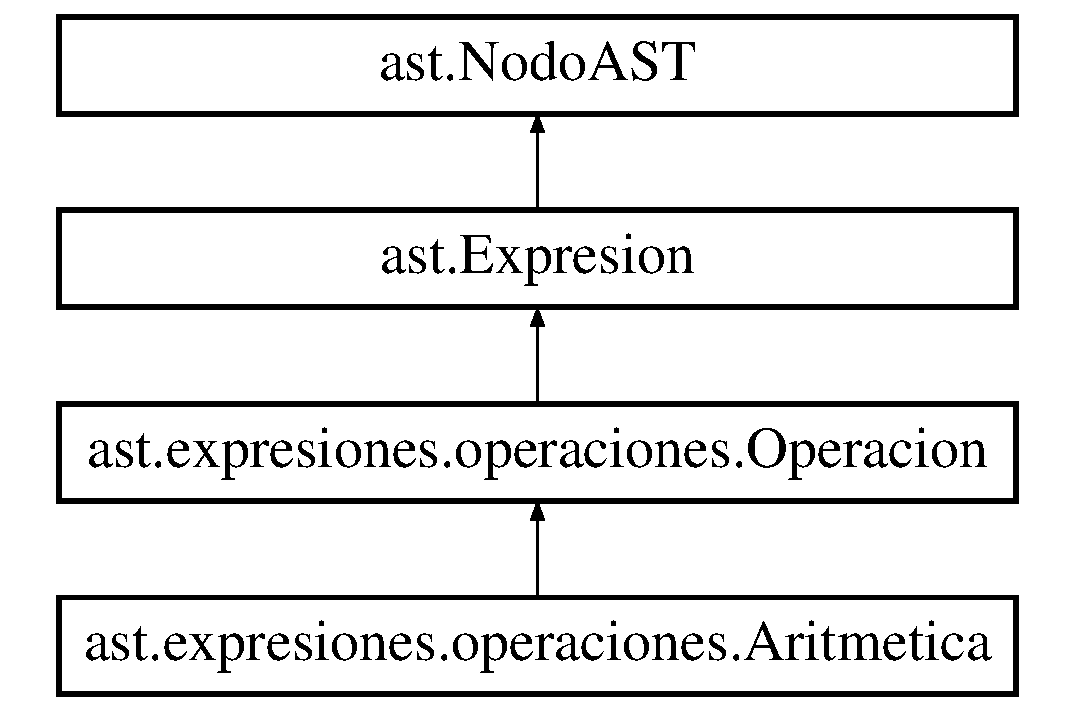
\includegraphics[height=4.000000cm]{classast_1_1expresiones_1_1operaciones_1_1_aritmetica}
\end{center}
\end{figure}
\subsection*{Public Member Functions}
\begin{DoxyCompactItemize}
\item 
\mbox{\Hypertarget{classast_1_1expresiones_1_1operaciones_1_1_aritmetica_a63e08fd38ba32ac188b3587ed1c397ea}\label{classast_1_1expresiones_1_1operaciones_1_1_aritmetica_a63e08fd38ba32ac188b3587ed1c397ea}} 
{\bfseries Aritmetica} (\mbox{\hyperlink{interfaceast_1_1_expresion}{Expresion}} op1, \mbox{\hyperlink{interfaceast_1_1_expresion}{Expresion}} op2, \mbox{\hyperlink{enumast_1_1expresiones_1_1operaciones_1_1_operacion_1_1_operador}{Operador}} operador, int col, int linea)
\item 
\mbox{\Hypertarget{classast_1_1expresiones_1_1operaciones_1_1_aritmetica_afb3cd0f634b1087642b9c83d42214249}\label{classast_1_1expresiones_1_1operaciones_1_1_aritmetica_afb3cd0f634b1087642b9c83d42214249}} 
{\bfseries Aritmetica} (\mbox{\hyperlink{interfaceast_1_1_expresion}{Expresion}} opU, \mbox{\hyperlink{enumast_1_1expresiones_1_1operaciones_1_1_operacion_1_1_operador}{Operador}} operador, int col, int linea)
\item 
\mbox{\Hypertarget{classast_1_1expresiones_1_1operaciones_1_1_aritmetica_a25b6fbd189ef258a170cbfd6acd58b21}\label{classast_1_1expresiones_1_1operaciones_1_1_aritmetica_a25b6fbd189ef258a170cbfd6acd58b21}} 
\mbox{\hyperlink{classentorno_1_1_tipo}{Tipo}} {\bfseries tipo\+Dominante} (\mbox{\hyperlink{classentorno_1_1_tipo}{Tipo}} t1, \mbox{\hyperlink{classentorno_1_1_tipo}{Tipo}} t2)
\item 
\mbox{\Hypertarget{classast_1_1expresiones_1_1operaciones_1_1_aritmetica_a603e643081004e93fbbd85c4c6030564}\label{classast_1_1expresiones_1_1operaciones_1_1_aritmetica_a603e643081004e93fbbd85c4c6030564}} 
\mbox{\hyperlink{classentorno_1_1_tipo}{Tipo}} {\bfseries get\+Tipo} (\mbox{\hyperlink{classentorno_1_1_entorno}{Entorno}} ent)
\item 
\mbox{\Hypertarget{classast_1_1expresiones_1_1operaciones_1_1_aritmetica_a4ff7d2a99104523f70679454c80449d0}\label{classast_1_1expresiones_1_1operaciones_1_1_aritmetica_a4ff7d2a99104523f70679454c80449d0}} 
Object {\bfseries get\+Valor\+Implicito} (\mbox{\hyperlink{classentorno_1_1_entorno}{Entorno}} ent)
\item 
\mbox{\Hypertarget{classast_1_1expresiones_1_1operaciones_1_1_aritmetica_a311c8c6028eb9c95cad1ea4363707547}\label{classast_1_1expresiones_1_1operaciones_1_1_aritmetica_a311c8c6028eb9c95cad1ea4363707547}} 
String {\bfseries get\+Nombre} (String\+Builder builder, String parent, int cont)
\end{DoxyCompactItemize}


\subsection{Detailed Description}
\begin{DoxyAuthor}{Author}
p\+\_\+ab1 
\end{DoxyAuthor}


The documentation for this class was generated from the following file\+:\begin{DoxyCompactItemize}
\item 
src/ast/expresiones/operaciones/Aritmetica.\+java\end{DoxyCompactItemize}

\hypertarget{classast_1_1instrucciones_1_1_asignacion}{}\section{ast.\+instrucciones.\+Asignacion Class Reference}
\label{classast_1_1instrucciones_1_1_asignacion}\index{ast.\+instrucciones.\+Asignacion@{ast.\+instrucciones.\+Asignacion}}
Inheritance diagram for ast.\+instrucciones.\+Asignacion\+:\begin{figure}[H]
\begin{center}
\leavevmode
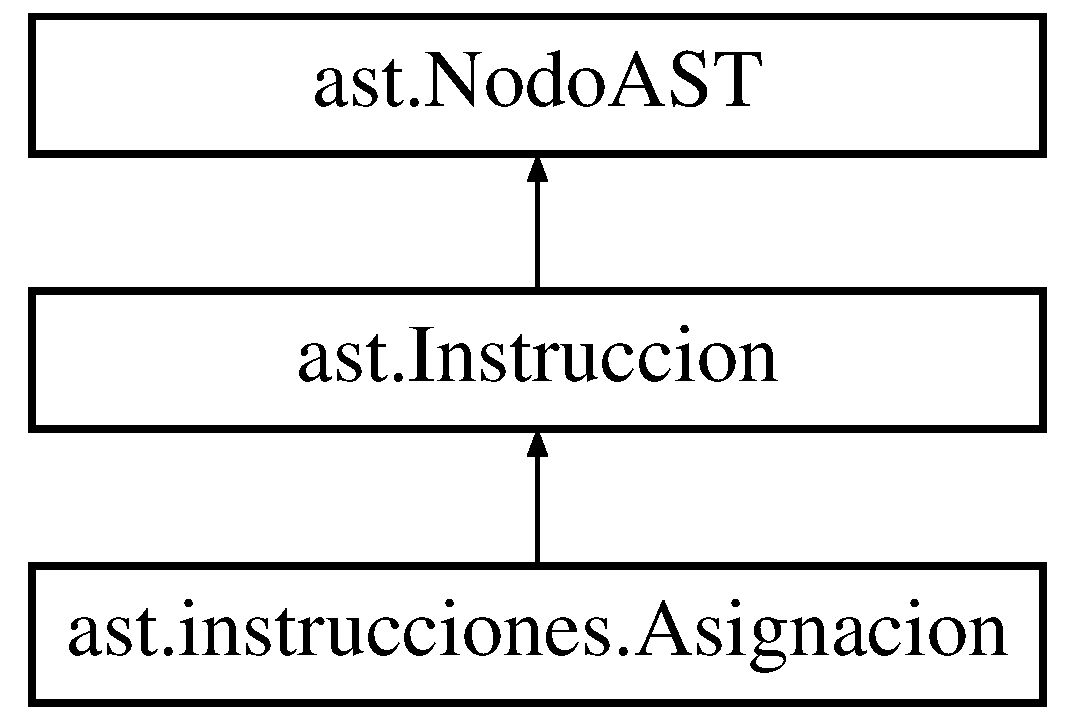
\includegraphics[height=3.000000cm]{classast_1_1instrucciones_1_1_asignacion}
\end{center}
\end{figure}
\subsection*{Public Member Functions}
\begin{DoxyCompactItemize}
\item 
\mbox{\Hypertarget{classast_1_1instrucciones_1_1_asignacion_ab6c0842d85fae9764e1e057fcf9aa23d}\label{classast_1_1instrucciones_1_1_asignacion_ab6c0842d85fae9764e1e057fcf9aa23d}} 
{\bfseries Asignacion} (\mbox{\hyperlink{interfaceast_1_1_expresion}{Expresion}} variable, \mbox{\hyperlink{interfaceast_1_1_expresion}{Expresion}} der, int linea, int col)
\item 
\mbox{\Hypertarget{classast_1_1instrucciones_1_1_asignacion_ae21cad9237c038de9adaf5dece31812f}\label{classast_1_1instrucciones_1_1_asignacion_ae21cad9237c038de9adaf5dece31812f}} 
\mbox{\hyperlink{interfaceast_1_1_expresion}{Expresion}} {\bfseries get\+Variable} ()
\item 
\mbox{\Hypertarget{classast_1_1instrucciones_1_1_asignacion_a51c388c932f0a15e3d85de33a2b3815b}\label{classast_1_1instrucciones_1_1_asignacion_a51c388c932f0a15e3d85de33a2b3815b}} 
void {\bfseries set\+Col} (int col)
\item 
\mbox{\Hypertarget{classast_1_1instrucciones_1_1_asignacion_afcc5b48c5e0896e772f0a2c932238dd9}\label{classast_1_1instrucciones_1_1_asignacion_afcc5b48c5e0896e772f0a2c932238dd9}} 
void {\bfseries set\+Linea} (int linea)
\item 
\mbox{\Hypertarget{classast_1_1instrucciones_1_1_asignacion_a4928c014ea18272088932d40fbf62d02}\label{classast_1_1instrucciones_1_1_asignacion_a4928c014ea18272088932d40fbf62d02}} 
Object {\bfseries ejecutar} (\mbox{\hyperlink{classentorno_1_1_entorno}{Entorno}} ent)
\item 
\mbox{\Hypertarget{classast_1_1instrucciones_1_1_asignacion_a854577e53808c11c41265c24afc095f6}\label{classast_1_1instrucciones_1_1_asignacion_a854577e53808c11c41265c24afc095f6}} 
int {\bfseries linea} ()
\item 
\mbox{\Hypertarget{classast_1_1instrucciones_1_1_asignacion_a2a43b9581bc35c2158decb47d2f0bc74}\label{classast_1_1instrucciones_1_1_asignacion_a2a43b9581bc35c2158decb47d2f0bc74}} 
int {\bfseries columna} ()
\item 
\mbox{\Hypertarget{classast_1_1instrucciones_1_1_asignacion_a60529ed6f9300c1016f46bad95a872df}\label{classast_1_1instrucciones_1_1_asignacion_a60529ed6f9300c1016f46bad95a872df}} 
String {\bfseries get\+Nombre} (String\+Builder builder, String parent, int cont)
\end{DoxyCompactItemize}


\subsection{Detailed Description}
\begin{DoxyAuthor}{Author}
p\+\_\+ab1 
\end{DoxyAuthor}


The documentation for this class was generated from the following file\+:\begin{DoxyCompactItemize}
\item 
src/ast/instrucciones/Asignacion.\+java\end{DoxyCompactItemize}

\hypertarget{classast_1_1_a_s_t}{}\section{ast.\+A\+ST Class Reference}
\label{classast_1_1_a_s_t}\index{ast.\+A\+ST@{ast.\+A\+ST}}
\subsection*{Public Member Functions}
\begin{DoxyCompactItemize}
\item 
\mbox{\Hypertarget{classast_1_1_a_s_t_a0170adf3b33b82d6a8669a9ff0b74ab9}\label{classast_1_1_a_s_t_a0170adf3b33b82d6a8669a9ff0b74ab9}} 
{\bfseries A\+ST} (Linked\+List$<$ \mbox{\hyperlink{interfaceast_1_1_nodo_a_s_t}{Nodo\+A\+ST}} $>$ instrucciones)
\item 
\mbox{\Hypertarget{classast_1_1_a_s_t_a6d567e4ad579c30a2911066522ce0e7e}\label{classast_1_1_a_s_t_a6d567e4ad579c30a2911066522ce0e7e}} 
\mbox{\hyperlink{classentorno_1_1_entorno}{Entorno}} {\bfseries get\+Global} ()
\item 
\mbox{\Hypertarget{classast_1_1_a_s_t_acbb06051ecbb65aa19e941a1ef6ed529}\label{classast_1_1_a_s_t_acbb06051ecbb65aa19e941a1ef6ed529}} 
Object {\bfseries ejecutar} ()
\item 
\mbox{\Hypertarget{classast_1_1_a_s_t_a195d73819c3a51a5f22a4f98f112a9f4}\label{classast_1_1_a_s_t_a195d73819c3a51a5f22a4f98f112a9f4}} 
Linked\+List$<$ \mbox{\hyperlink{interfaceast_1_1_nodo_a_s_t}{Nodo\+A\+ST}} $>$ {\bfseries get\+Instrucciones} ()
\item 
\mbox{\Hypertarget{classast_1_1_a_s_t_a769b18dc96965567424b4cd557166ba9}\label{classast_1_1_a_s_t_a769b18dc96965567424b4cd557166ba9}} 
void {\bfseries set\+Instrucciones} (Linked\+List$<$ \mbox{\hyperlink{interfaceast_1_1_nodo_a_s_t}{Nodo\+A\+ST}} $>$ instrucciones)
\item 
\mbox{\Hypertarget{classast_1_1_a_s_t_a7f988b92f6b374530103eb57584ede90}\label{classast_1_1_a_s_t_a7f988b92f6b374530103eb57584ede90}} 
String {\bfseries Graficar} ()
\end{DoxyCompactItemize}


\subsection{Detailed Description}
\begin{DoxyAuthor}{Author}
p\+\_\+ab1 
\end{DoxyAuthor}


The documentation for this class was generated from the following file\+:\begin{DoxyCompactItemize}
\item 
src/ast/A\+S\+T.\+java\end{DoxyCompactItemize}

\hypertarget{classast_1_1instrucciones_1_1_break}{}\section{ast.\+instrucciones.\+Break Class Reference}
\label{classast_1_1instrucciones_1_1_break}\index{ast.\+instrucciones.\+Break@{ast.\+instrucciones.\+Break}}
Inheritance diagram for ast.\+instrucciones.\+Break\+:\begin{figure}[H]
\begin{center}
\leavevmode
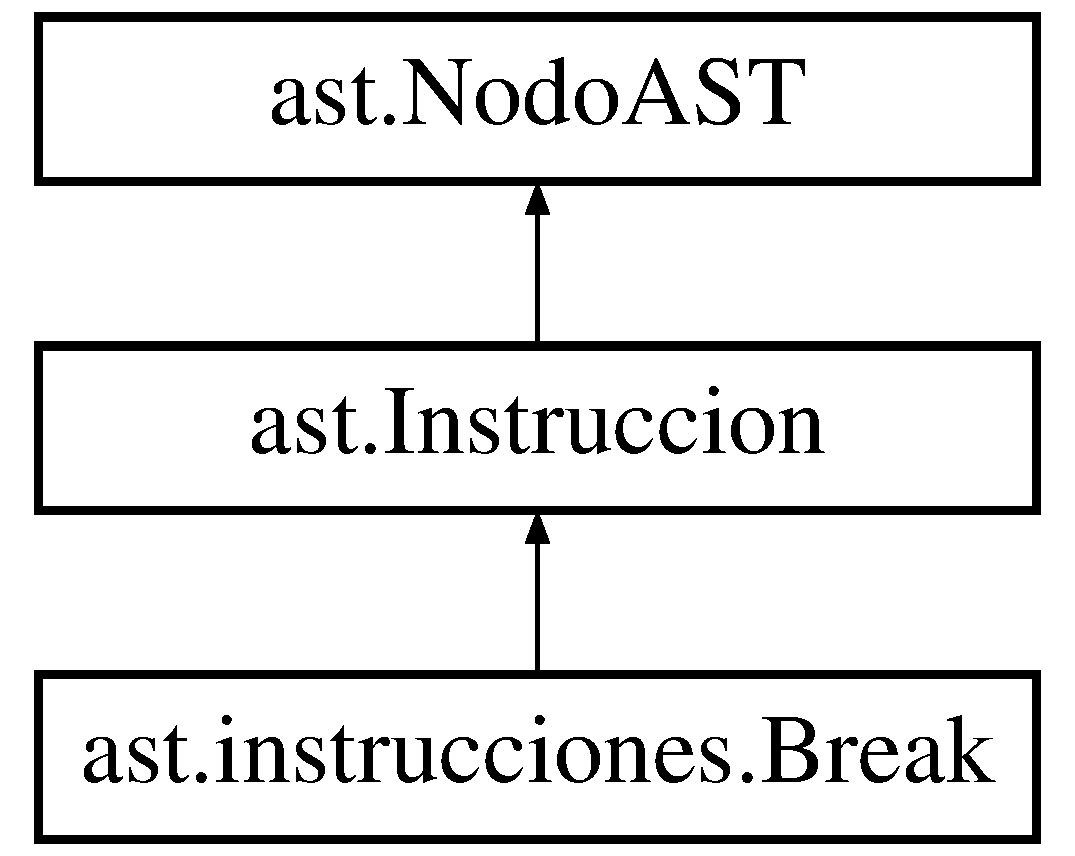
\includegraphics[height=3.000000cm]{classast_1_1instrucciones_1_1_break}
\end{center}
\end{figure}
\subsection*{Public Member Functions}
\begin{DoxyCompactItemize}
\item 
\mbox{\Hypertarget{classast_1_1instrucciones_1_1_break_a5cf514c19c9c87dad49ce5e21035e9ab}\label{classast_1_1instrucciones_1_1_break_a5cf514c19c9c87dad49ce5e21035e9ab}} 
{\bfseries Break} (int linea, int col)
\item 
\mbox{\Hypertarget{classast_1_1instrucciones_1_1_break_a7d018447eda1feae75640013de6acb70}\label{classast_1_1instrucciones_1_1_break_a7d018447eda1feae75640013de6acb70}} 
Object {\bfseries ejecutar} (\mbox{\hyperlink{classentorno_1_1_entorno}{Entorno}} ent)
\item 
\mbox{\Hypertarget{classast_1_1instrucciones_1_1_break_a15d547f54c9a2ad34aaaa73dbec08ae8}\label{classast_1_1instrucciones_1_1_break_a15d547f54c9a2ad34aaaa73dbec08ae8}} 
int {\bfseries linea} ()
\item 
\mbox{\Hypertarget{classast_1_1instrucciones_1_1_break_a2bd8cf63d79ecf73d4718020276090eb}\label{classast_1_1instrucciones_1_1_break_a2bd8cf63d79ecf73d4718020276090eb}} 
int {\bfseries columna} ()
\item 
\mbox{\Hypertarget{classast_1_1instrucciones_1_1_break_a96d3cb843c1b32146dbcbfd280ccef97}\label{classast_1_1instrucciones_1_1_break_a96d3cb843c1b32146dbcbfd280ccef97}} 
String {\bfseries get\+Nombre} (String\+Builder builder, String parent, int cont)
\end{DoxyCompactItemize}


\subsection{Detailed Description}
\begin{DoxyAuthor}{Author}
p\+\_\+ab1 
\end{DoxyAuthor}


The documentation for this class was generated from the following file\+:\begin{DoxyCompactItemize}
\item 
src/ast/instrucciones/Break.\+java\end{DoxyCompactItemize}

\hypertarget{classast_1_1instrucciones_1_1_condicion}{}\section{ast.\+instrucciones.\+Condicion Class Reference}
\label{classast_1_1instrucciones_1_1_condicion}\index{ast.\+instrucciones.\+Condicion@{ast.\+instrucciones.\+Condicion}}
Inheritance diagram for ast.\+instrucciones.\+Condicion\+:\begin{figure}[H]
\begin{center}
\leavevmode
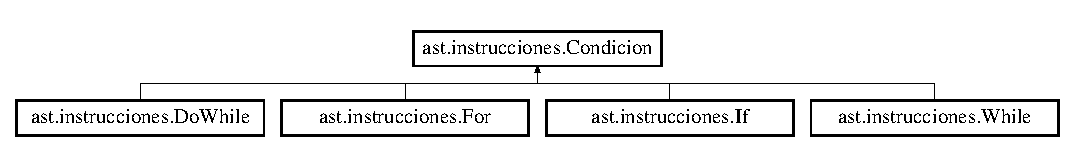
\includegraphics[height=1.590909cm]{classast_1_1instrucciones_1_1_condicion}
\end{center}
\end{figure}
\subsection*{Public Member Functions}
\begin{DoxyCompactItemize}
\item 
\mbox{\Hypertarget{classast_1_1instrucciones_1_1_condicion_a43fdc245eca24b92896e5360e8766115}\label{classast_1_1instrucciones_1_1_condicion_a43fdc245eca24b92896e5360e8766115}} 
{\bfseries Condicion} (Linked\+List$<$ \mbox{\hyperlink{interfaceast_1_1_nodo_a_s_t}{Nodo\+A\+ST}} $>$ ins, \mbox{\hyperlink{interfaceast_1_1_expresion}{Expresion}} cond)
\item 
\mbox{\Hypertarget{classast_1_1instrucciones_1_1_condicion_ab60c28ffc28109159254190967642ecd}\label{classast_1_1instrucciones_1_1_condicion_ab60c28ffc28109159254190967642ecd}} 
Linked\+List$<$ \mbox{\hyperlink{interfaceast_1_1_nodo_a_s_t}{Nodo\+A\+ST}} $>$ {\bfseries get\+Ins} ()
\item 
\mbox{\Hypertarget{classast_1_1instrucciones_1_1_condicion_a47eb8d8b9b43773e1711b8d57c2623bc}\label{classast_1_1instrucciones_1_1_condicion_a47eb8d8b9b43773e1711b8d57c2623bc}} 
void {\bfseries set\+Ins} (Linked\+List$<$ \mbox{\hyperlink{interfaceast_1_1_nodo_a_s_t}{Nodo\+A\+ST}} $>$ ins)
\item 
\mbox{\Hypertarget{classast_1_1instrucciones_1_1_condicion_a38aa1ed6dc8b60c6ac16b073ae64c87a}\label{classast_1_1instrucciones_1_1_condicion_a38aa1ed6dc8b60c6ac16b073ae64c87a}} 
\mbox{\hyperlink{interfaceast_1_1_expresion}{Expresion}} {\bfseries get\+Cond} ()
\item 
\mbox{\Hypertarget{classast_1_1instrucciones_1_1_condicion_aafab95a5ec504c624f5d1854295a08ea}\label{classast_1_1instrucciones_1_1_condicion_aafab95a5ec504c624f5d1854295a08ea}} 
void {\bfseries set\+Cond} (\mbox{\hyperlink{interfaceast_1_1_expresion}{Expresion}} cond)
\end{DoxyCompactItemize}


\subsection{Detailed Description}
\begin{DoxyAuthor}{Author}
p\+\_\+ab1 
\end{DoxyAuthor}


The documentation for this class was generated from the following file\+:\begin{DoxyCompactItemize}
\item 
src/ast/instrucciones/Condicion.\+java\end{DoxyCompactItemize}

\hypertarget{classast_1_1instrucciones_1_1_continue}{}\section{ast.\+instrucciones.\+Continue Class Reference}
\label{classast_1_1instrucciones_1_1_continue}\index{ast.\+instrucciones.\+Continue@{ast.\+instrucciones.\+Continue}}
Inheritance diagram for ast.\+instrucciones.\+Continue\+:\begin{figure}[H]
\begin{center}
\leavevmode
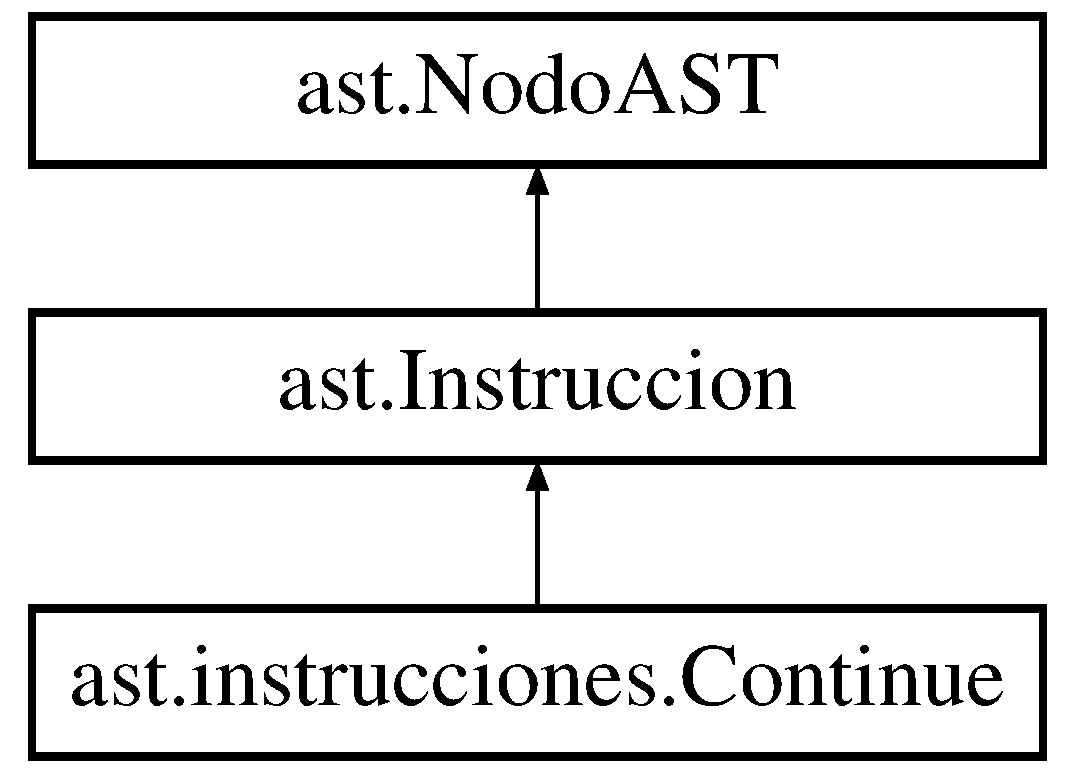
\includegraphics[height=3.000000cm]{classast_1_1instrucciones_1_1_continue}
\end{center}
\end{figure}
\subsection*{Public Member Functions}
\begin{DoxyCompactItemize}
\item 
\mbox{\Hypertarget{classast_1_1instrucciones_1_1_continue_ac7ef7c94a32e7857df71347123812d72}\label{classast_1_1instrucciones_1_1_continue_ac7ef7c94a32e7857df71347123812d72}} 
{\bfseries Continue} (int linea, int col)
\item 
\mbox{\Hypertarget{classast_1_1instrucciones_1_1_continue_a27917e95b57605360e538ee6301a13ee}\label{classast_1_1instrucciones_1_1_continue_a27917e95b57605360e538ee6301a13ee}} 
Object {\bfseries ejecutar} (\mbox{\hyperlink{classentorno_1_1_entorno}{Entorno}} ent)
\item 
\mbox{\Hypertarget{classast_1_1instrucciones_1_1_continue_a13058684f74e61d1e8093907645e3726}\label{classast_1_1instrucciones_1_1_continue_a13058684f74e61d1e8093907645e3726}} 
int {\bfseries linea} ()
\item 
\mbox{\Hypertarget{classast_1_1instrucciones_1_1_continue_a2f41948b20f2546f18e176ad4a108be6}\label{classast_1_1instrucciones_1_1_continue_a2f41948b20f2546f18e176ad4a108be6}} 
String {\bfseries get\+Nombre} (String\+Builder builder, String parent, int cont)
\item 
\mbox{\Hypertarget{classast_1_1instrucciones_1_1_continue_ad7ed0a53345e43687780fb66ac028976}\label{classast_1_1instrucciones_1_1_continue_ad7ed0a53345e43687780fb66ac028976}} 
int {\bfseries columna} ()
\end{DoxyCompactItemize}


\subsection{Detailed Description}
\begin{DoxyAuthor}{Author}
p\+\_\+ab1 
\end{DoxyAuthor}


The documentation for this class was generated from the following file\+:\begin{DoxyCompactItemize}
\item 
src/ast/instrucciones/Continue.\+java\end{DoxyCompactItemize}

\hypertarget{classast_1_1instrucciones_1_1_do_while}{}\section{ast.\+instrucciones.\+Do\+While Class Reference}
\label{classast_1_1instrucciones_1_1_do_while}\index{ast.\+instrucciones.\+Do\+While@{ast.\+instrucciones.\+Do\+While}}
Inheritance diagram for ast.\+instrucciones.\+Do\+While\+:\begin{figure}[H]
\begin{center}
\leavevmode
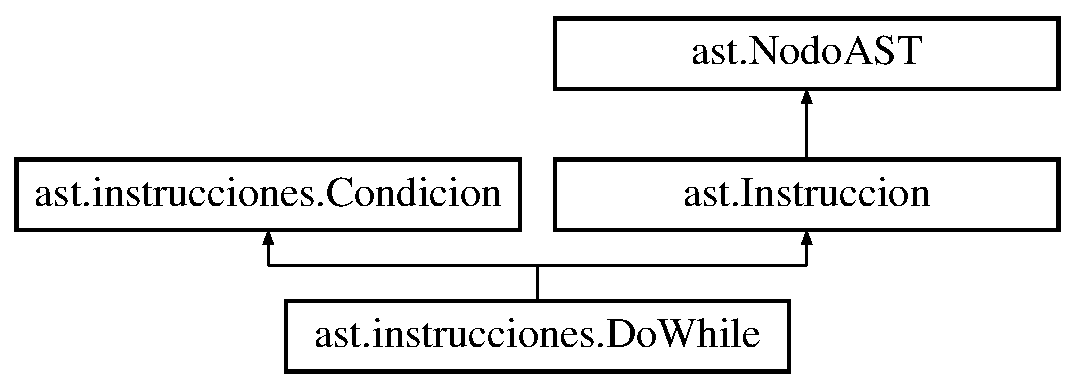
\includegraphics[height=3.000000cm]{classast_1_1instrucciones_1_1_do_while}
\end{center}
\end{figure}
\subsection*{Public Member Functions}
\begin{DoxyCompactItemize}
\item 
\mbox{\Hypertarget{classast_1_1instrucciones_1_1_do_while_a0f10c5f88ef45feb5e1aa0d5e1cc247e}\label{classast_1_1instrucciones_1_1_do_while_a0f10c5f88ef45feb5e1aa0d5e1cc247e}} 
{\bfseries Do\+While} (Linked\+List$<$ \mbox{\hyperlink{interfaceast_1_1_nodo_a_s_t}{Nodo\+A\+ST}} $>$ ins, \mbox{\hyperlink{interfaceast_1_1_expresion}{Expresion}} cond, int lin, int col)
\item 
\mbox{\Hypertarget{classast_1_1instrucciones_1_1_do_while_a8bf678c02671621f7f29f75d8f8a78ae}\label{classast_1_1instrucciones_1_1_do_while_a8bf678c02671621f7f29f75d8f8a78ae}} 
Object {\bfseries ejecutar} (\mbox{\hyperlink{classentorno_1_1_entorno}{Entorno}} ent)
\item 
\mbox{\Hypertarget{classast_1_1instrucciones_1_1_do_while_a9cd464bcac563581af14d5aea3fd5e89}\label{classast_1_1instrucciones_1_1_do_while_a9cd464bcac563581af14d5aea3fd5e89}} 
int {\bfseries linea} ()
\item 
\mbox{\Hypertarget{classast_1_1instrucciones_1_1_do_while_aec03ae07f47565f34a68f68679c217b3}\label{classast_1_1instrucciones_1_1_do_while_aec03ae07f47565f34a68f68679c217b3}} 
int {\bfseries columna} ()
\item 
\mbox{\Hypertarget{classast_1_1instrucciones_1_1_do_while_abc8cdc79a0a9a46b794c1001d9cb5cba}\label{classast_1_1instrucciones_1_1_do_while_abc8cdc79a0a9a46b794c1001d9cb5cba}} 
String {\bfseries get\+Nombre} (String\+Builder builder, String parent, int cont)
\end{DoxyCompactItemize}


\subsection{Detailed Description}
\begin{DoxyAuthor}{Author}
p\+\_\+ab1 
\end{DoxyAuthor}


The documentation for this class was generated from the following file\+:\begin{DoxyCompactItemize}
\item 
src/ast/instrucciones/Do\+While.\+java\end{DoxyCompactItemize}

\hypertarget{classolc2_1_1p1__201504242_1_1_editor}{}\section{olc2.\+p1\+\_\+201504242.\+Editor Class Reference}
\label{classolc2_1_1p1__201504242_1_1_editor}\index{olc2.\+p1\+\_\+201504242.\+Editor@{olc2.\+p1\+\_\+201504242.\+Editor}}
Inheritance diagram for olc2.\+p1\+\_\+201504242.\+Editor\+:\begin{figure}[H]
\begin{center}
\leavevmode
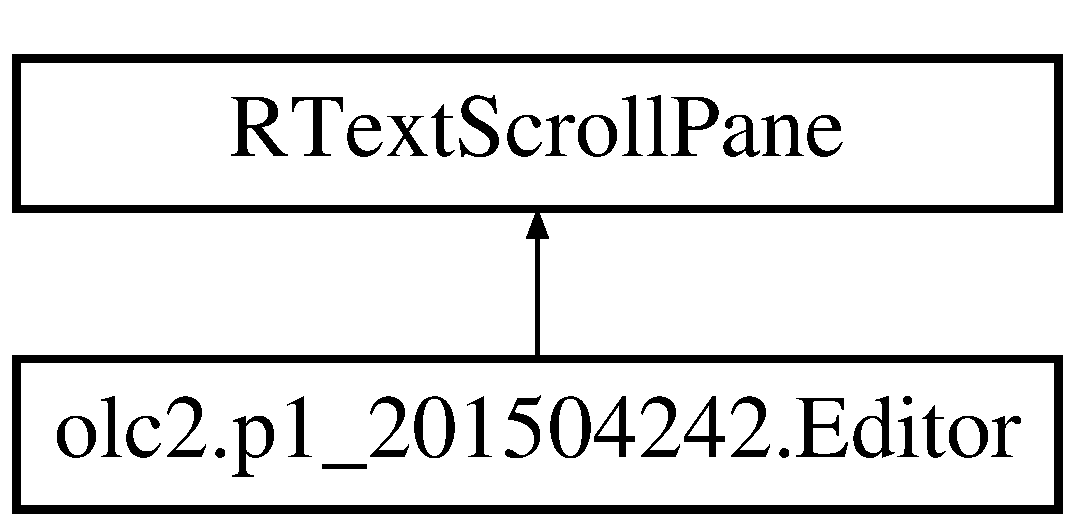
\includegraphics[height=2.000000cm]{classolc2_1_1p1__201504242_1_1_editor}
\end{center}
\end{figure}
\subsection*{Public Member Functions}
\begin{DoxyCompactItemize}
\item 
\mbox{\Hypertarget{classolc2_1_1p1__201504242_1_1_editor_ae450ebb2ac12b7ca86ec857262234d54}\label{classolc2_1_1p1__201504242_1_1_editor_ae450ebb2ac12b7ca86ec857262234d54}} 
{\bfseries Editor} (File archivo, R\+Syntax\+Text\+Area text)  throws File\+Not\+Found\+Exception, I\+O\+Exception     
\item 
\mbox{\Hypertarget{classolc2_1_1p1__201504242_1_1_editor_a7d8e9510d153eebf0c72edfa25f6a007}\label{classolc2_1_1p1__201504242_1_1_editor_a7d8e9510d153eebf0c72edfa25f6a007}} 
{\bfseries Editor} (R\+Syntax\+Text\+Area text)  throws File\+Not\+Found\+Exception, I\+O\+Exception     
\item 
\mbox{\Hypertarget{classolc2_1_1p1__201504242_1_1_editor_aec577468b98cbe6c7638f673b7afd60e}\label{classolc2_1_1p1__201504242_1_1_editor_aec577468b98cbe6c7638f673b7afd60e}} 
String {\bfseries get\+Recurso} ()
\item 
\mbox{\Hypertarget{classolc2_1_1p1__201504242_1_1_editor_a7072dda437e6315799e3a01911cce0fe}\label{classolc2_1_1p1__201504242_1_1_editor_a7072dda437e6315799e3a01911cce0fe}} 
String {\bfseries get\+Titulo} ()
\item 
\mbox{\Hypertarget{classolc2_1_1p1__201504242_1_1_editor_af7f0afcfb653c45fdf48c25527b513c9}\label{classolc2_1_1p1__201504242_1_1_editor_af7f0afcfb653c45fdf48c25527b513c9}} 
String {\bfseries get\+Codigo} ()
\item 
\mbox{\Hypertarget{classolc2_1_1p1__201504242_1_1_editor_a2976a68ad6b7656e7345a30e9531654e}\label{classolc2_1_1p1__201504242_1_1_editor_a2976a68ad6b7656e7345a30e9531654e}} 
void {\bfseries set\+Codigo} (String codigo)
\end{DoxyCompactItemize}


\subsection{Detailed Description}
\begin{DoxyAuthor}{Author}
Jorge 
\end{DoxyAuthor}


The documentation for this class was generated from the following file\+:\begin{DoxyCompactItemize}
\item 
src/olc2/p1\+\_\+201504242/Editor.\+java\end{DoxyCompactItemize}

\hypertarget{classentorno_1_1_entorno}{}\section{entorno.\+Entorno Class Reference}
\label{classentorno_1_1_entorno}\index{entorno.\+Entorno@{entorno.\+Entorno}}
\subsection*{Public Member Functions}
\begin{DoxyCompactItemize}
\item 
\mbox{\Hypertarget{classentorno_1_1_entorno_a7a0843748c778ddb94aa815d28c41536}\label{classentorno_1_1_entorno_a7a0843748c778ddb94aa815d28c41536}} 
{\bfseries Entorno} (\mbox{\hyperlink{classentorno_1_1_entorno}{Entorno}} anterior)
\item 
\mbox{\Hypertarget{classentorno_1_1_entorno_a8b196372a177862e71bcdc9c0193b391}\label{classentorno_1_1_entorno_a8b196372a177862e71bcdc9c0193b391}} 
void {\bfseries agregar} (String id, \mbox{\hyperlink{classentorno_1_1_simbolo}{Simbolo}} simbolo)
\item 
\mbox{\Hypertarget{classentorno_1_1_entorno_a49e07a304315b92414630ecaca7e56ea}\label{classentorno_1_1_entorno_a49e07a304315b92414630ecaca7e56ea}} 
void {\bfseries agregar\+Funcion} (String id, \mbox{\hyperlink{classentorno_1_1_simbolo}{Simbolo}} simbolo)
\item 
\mbox{\Hypertarget{classentorno_1_1_entorno_ab7a2724644ae90bbc9e620049c829b9e}\label{classentorno_1_1_entorno_ab7a2724644ae90bbc9e620049c829b9e}} 
\mbox{\hyperlink{classentorno_1_1_simbolo}{Simbolo}} {\bfseries get} (String id)
\item 
\mbox{\Hypertarget{classentorno_1_1_entorno_a08eb0a0347adda9f40bcb776c701e361}\label{classentorno_1_1_entorno_a08eb0a0347adda9f40bcb776c701e361}} 
\mbox{\hyperlink{classentorno_1_1_simbolo}{Simbolo}} {\bfseries get\+Funcion} (String id)
\item 
\mbox{\Hypertarget{classentorno_1_1_entorno_a4ba0e65ae77a0bbb439dcf064d6be983}\label{classentorno_1_1_entorno_a4ba0e65ae77a0bbb439dcf064d6be983}} 
void {\bfseries reemplazar} (String id, \mbox{\hyperlink{classentorno_1_1_simbolo}{Simbolo}} nuevo\+Valor)
\item 
\mbox{\Hypertarget{classentorno_1_1_entorno_ac03c40600e1cab9d8d946fd6f1cfad60}\label{classentorno_1_1_entorno_ac03c40600e1cab9d8d946fd6f1cfad60}} 
void {\bfseries reemplazar\+Fun} (String id, \mbox{\hyperlink{classentorno_1_1_simbolo}{Simbolo}} nuevo\+Valor)
\item 
\mbox{\Hypertarget{classentorno_1_1_entorno_a706feef9251a7f4bac0a72a401b358bb}\label{classentorno_1_1_entorno_a706feef9251a7f4bac0a72a401b358bb}} 
void {\bfseries Mostrar} ()
\item 
\mbox{\Hypertarget{classentorno_1_1_entorno_af5def864db6d045fbc2df78d810985ff}\label{classentorno_1_1_entorno_af5def864db6d045fbc2df78d810985ff}} 
boolean {\bfseries existe} (String id)
\item 
\mbox{\Hypertarget{classentorno_1_1_entorno_adf774e0bfcc00081aa03a8d4acd03421}\label{classentorno_1_1_entorno_adf774e0bfcc00081aa03a8d4acd03421}} 
boolean {\bfseries existe\+Funcion} (String id)
\item 
\mbox{\Hypertarget{classentorno_1_1_entorno_ad190dca46a47bf719b8b0a39bf684188}\label{classentorno_1_1_entorno_ad190dca46a47bf719b8b0a39bf684188}} 
boolean {\bfseries existe\+En\+Actual} (String id)
\item 
\mbox{\Hypertarget{classentorno_1_1_entorno_a7053d407b670dce82e1b5579e3b79c98}\label{classentorno_1_1_entorno_a7053d407b670dce82e1b5579e3b79c98}} 
Hashtable {\bfseries get\+Tabla} ()
\item 
\mbox{\Hypertarget{classentorno_1_1_entorno_a3b2f7f0ba287916fd68b7c85e60a9d8d}\label{classentorno_1_1_entorno_a3b2f7f0ba287916fd68b7c85e60a9d8d}} 
void {\bfseries set\+Tabla} (Hashtable tabla)
\item 
\mbox{\Hypertarget{classentorno_1_1_entorno_a9d6c3e60aa6db7f0daef65b200eb2b10}\label{classentorno_1_1_entorno_a9d6c3e60aa6db7f0daef65b200eb2b10}} 
\mbox{\hyperlink{classentorno_1_1_entorno}{Entorno}} {\bfseries get\+Anterior} ()
\item 
\mbox{\Hypertarget{classentorno_1_1_entorno_a5ffd51f75210a71b1b7e38d37625a1c1}\label{classentorno_1_1_entorno_a5ffd51f75210a71b1b7e38d37625a1c1}} 
void {\bfseries set\+Anterior} (\mbox{\hyperlink{classentorno_1_1_entorno}{Entorno}} anterior)
\item 
\mbox{\Hypertarget{classentorno_1_1_entorno_a00229948ef8e3b50341a46fc76be2aa6}\label{classentorno_1_1_entorno_a00229948ef8e3b50341a46fc76be2aa6}} 
void {\bfseries Mostrar\+Funciones} ()
\item 
\mbox{\Hypertarget{classentorno_1_1_entorno_a09ac19c76b5c3a9bfddfade4624c920a}\label{classentorno_1_1_entorno_a09ac19c76b5c3a9bfddfade4624c920a}} 
Hashtable {\bfseries get\+Funciones} ()
\end{DoxyCompactItemize}


\subsection{Detailed Description}
\begin{DoxyAuthor}{Author}
p\+\_\+ab1 
\end{DoxyAuthor}


The documentation for this class was generated from the following file\+:\begin{DoxyCompactItemize}
\item 
src/entorno/Entorno.\+java\end{DoxyCompactItemize}

\hypertarget{interfaceast_1_1_expresion}{}\section{ast.\+Expresion Interface Reference}
\label{interfaceast_1_1_expresion}\index{ast.\+Expresion@{ast.\+Expresion}}
Inheritance diagram for ast.\+Expresion\+:\begin{figure}[H]
\begin{center}
\leavevmode
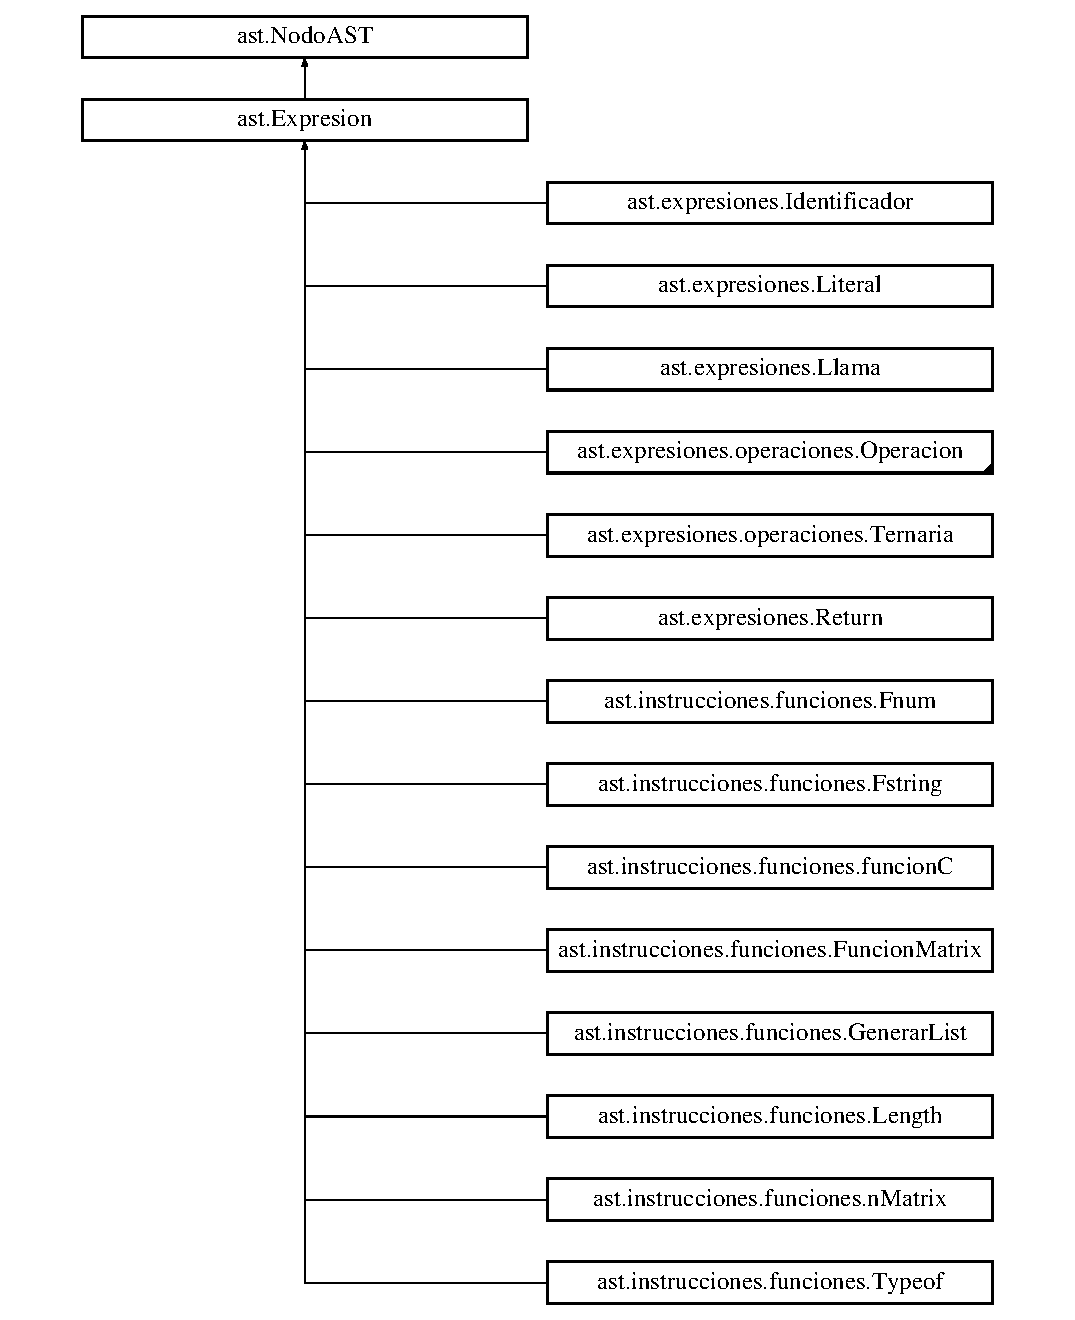
\includegraphics[height=12.000000cm]{interfaceast_1_1_expresion}
\end{center}
\end{figure}
\subsection*{Public Member Functions}
\begin{DoxyCompactItemize}
\item 
\mbox{\Hypertarget{interfaceast_1_1_expresion_a514776885f5a1d95ce239ff1da48fe81}\label{interfaceast_1_1_expresion_a514776885f5a1d95ce239ff1da48fe81}} 
\mbox{\hyperlink{classentorno_1_1_tipo}{Tipo}} {\bfseries get\+Tipo} (\mbox{\hyperlink{classentorno_1_1_entorno}{Entorno}} ent)
\item 
\mbox{\Hypertarget{interfaceast_1_1_expresion_a098f8589cd4dc84f7d76b4958e2418f1}\label{interfaceast_1_1_expresion_a098f8589cd4dc84f7d76b4958e2418f1}} 
Object {\bfseries get\+Valor\+Implicito} (\mbox{\hyperlink{classentorno_1_1_entorno}{Entorno}} ent)
\end{DoxyCompactItemize}


\subsection{Detailed Description}
\begin{DoxyAuthor}{Author}
p\+\_\+ab1 
\end{DoxyAuthor}


The documentation for this interface was generated from the following file\+:\begin{DoxyCompactItemize}
\item 
src/ast/Expresion.\+java\end{DoxyCompactItemize}

\hypertarget{classentorno_1_1fantasmita}{}\section{entorno.\+fantasmita Class Reference}
\label{classentorno_1_1fantasmita}\index{entorno.\+fantasmita@{entorno.\+fantasmita}}
Inheritance diagram for entorno.\+fantasmita\+:\begin{figure}[H]
\begin{center}
\leavevmode
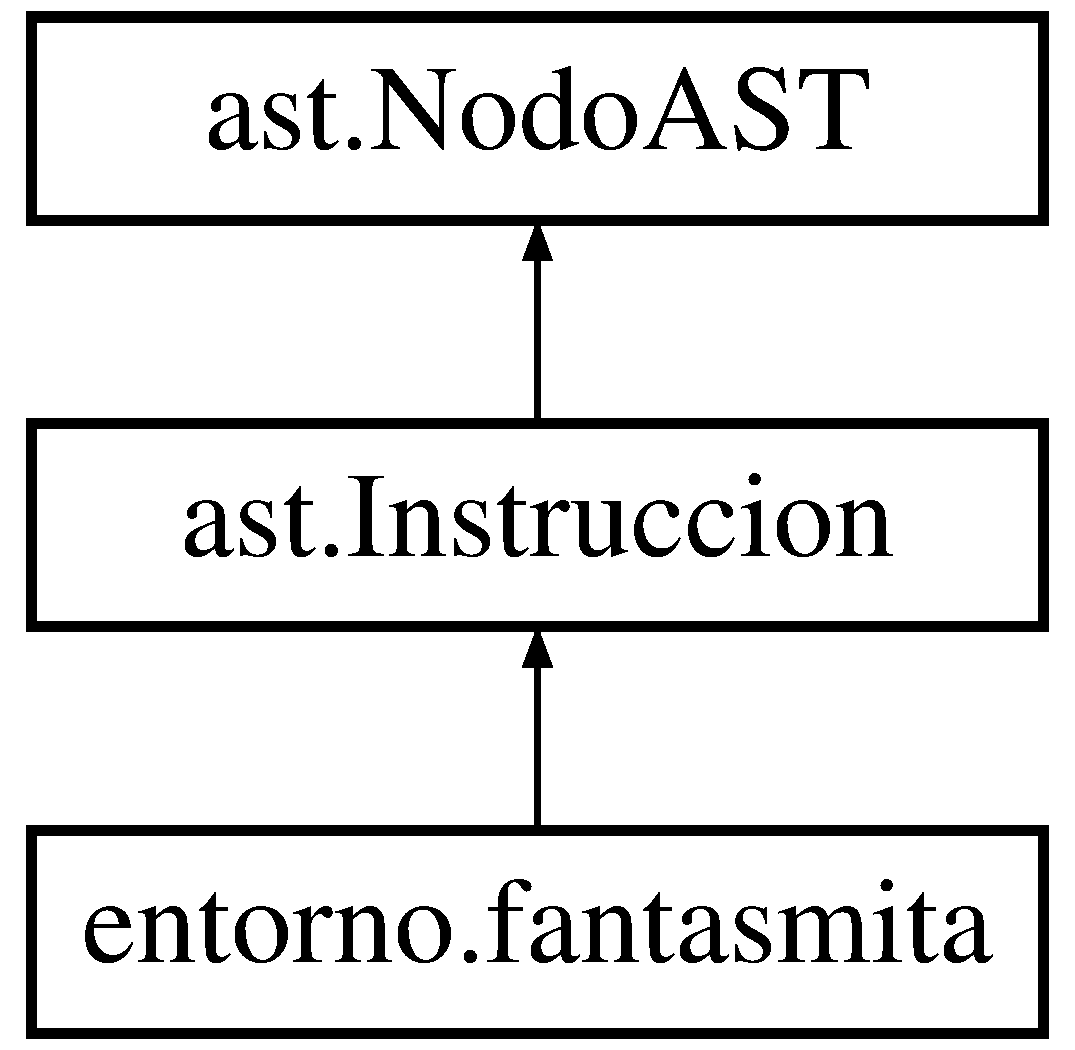
\includegraphics[height=3.000000cm]{classentorno_1_1fantasmita}
\end{center}
\end{figure}
\subsection*{Public Member Functions}
\begin{DoxyCompactItemize}
\item 
\mbox{\Hypertarget{classentorno_1_1fantasmita_a39704709c1f52ea0303d42f45f27fdf0}\label{classentorno_1_1fantasmita_a39704709c1f52ea0303d42f45f27fdf0}} 
Object {\bfseries ejecutar} (\mbox{\hyperlink{classentorno_1_1_entorno}{Entorno}} ent)
\item 
\mbox{\Hypertarget{classentorno_1_1fantasmita_a951a0e24728b438e6ee39d397891c423}\label{classentorno_1_1fantasmita_a951a0e24728b438e6ee39d397891c423}} 
int {\bfseries linea} ()
\item 
\mbox{\Hypertarget{classentorno_1_1fantasmita_a4a79c441d99a4183defe3b8c2a624585}\label{classentorno_1_1fantasmita_a4a79c441d99a4183defe3b8c2a624585}} 
int {\bfseries columna} ()
\item 
\mbox{\Hypertarget{classentorno_1_1fantasmita_aac4bf54c18db48a4851829c729afd2fa}\label{classentorno_1_1fantasmita_aac4bf54c18db48a4851829c729afd2fa}} 
String {\bfseries get\+Nombre} (String\+Builder builder, String parent, int cont)
\end{DoxyCompactItemize}


\subsection{Detailed Description}
\begin{DoxyAuthor}{Author}
p\+\_\+ab1 
\end{DoxyAuthor}


The documentation for this class was generated from the following file\+:\begin{DoxyCompactItemize}
\item 
src/entorno/fantasmita.\+java\end{DoxyCompactItemize}

\hypertarget{classast_1_1instrucciones_1_1funciones_1_1_fnum}{}\section{ast.\+instrucciones.\+funciones.\+Fnum Class Reference}
\label{classast_1_1instrucciones_1_1funciones_1_1_fnum}\index{ast.\+instrucciones.\+funciones.\+Fnum@{ast.\+instrucciones.\+funciones.\+Fnum}}
Inheritance diagram for ast.\+instrucciones.\+funciones.\+Fnum\+:\begin{figure}[H]
\begin{center}
\leavevmode
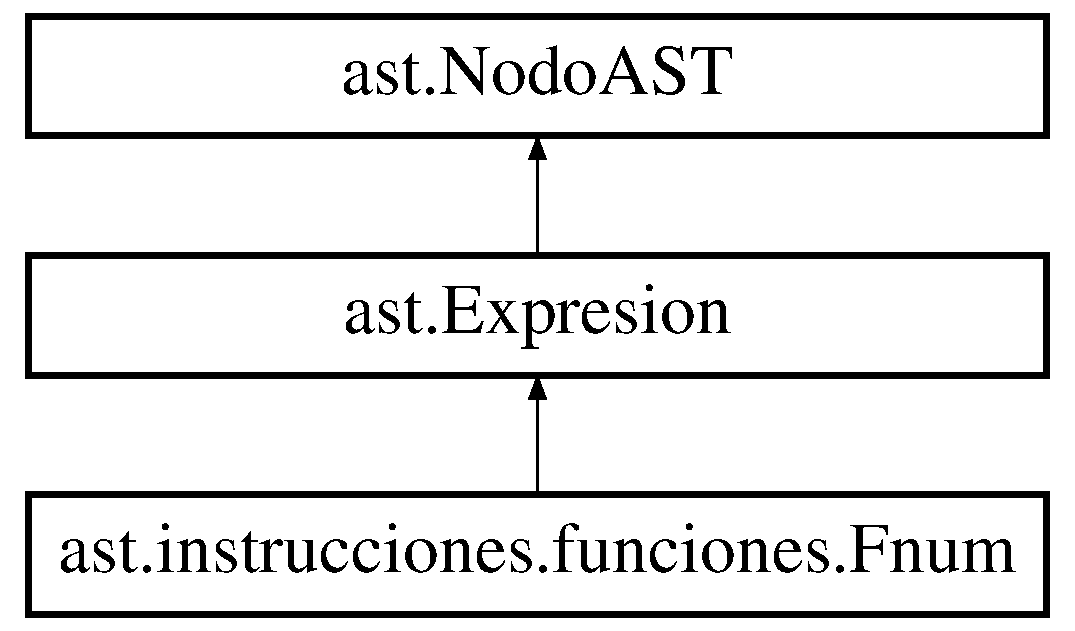
\includegraphics[height=3.000000cm]{classast_1_1instrucciones_1_1funciones_1_1_fnum}
\end{center}
\end{figure}
\subsection*{Public Member Functions}
\begin{DoxyCompactItemize}
\item 
\mbox{\Hypertarget{classast_1_1instrucciones_1_1funciones_1_1_fnum_adf2741c04f22e8e9006fb86240c54446}\label{classast_1_1instrucciones_1_1funciones_1_1_fnum_adf2741c04f22e8e9006fb86240c54446}} 
{\bfseries Fnum} (int tipo, Linked\+List$<$ \mbox{\hyperlink{interfaceast_1_1_nodo_a_s_t}{Nodo\+A\+ST}} $>$ valor, int linea, int col)
\item 
\mbox{\Hypertarget{classast_1_1instrucciones_1_1funciones_1_1_fnum_a34ffed52627de5c5d3d9eb53bbac0a94}\label{classast_1_1instrucciones_1_1funciones_1_1_fnum_a34ffed52627de5c5d3d9eb53bbac0a94}} 
\mbox{\hyperlink{classentorno_1_1_tipo}{Tipo}} {\bfseries get\+Tipo} (\mbox{\hyperlink{classentorno_1_1_entorno}{Entorno}} ent)
\item 
\mbox{\Hypertarget{classast_1_1instrucciones_1_1funciones_1_1_fnum_a78ac3f050bc27ce8487ea4b8c2673619}\label{classast_1_1instrucciones_1_1funciones_1_1_fnum_a78ac3f050bc27ce8487ea4b8c2673619}} 
Object {\bfseries get\+Valor\+Implicito} (\mbox{\hyperlink{classentorno_1_1_entorno}{Entorno}} ent)
\item 
\mbox{\Hypertarget{classast_1_1instrucciones_1_1funciones_1_1_fnum_a9b96b33766dbc222ead407a663fafaec}\label{classast_1_1instrucciones_1_1funciones_1_1_fnum_a9b96b33766dbc222ead407a663fafaec}} 
int {\bfseries linea} ()
\item 
\mbox{\Hypertarget{classast_1_1instrucciones_1_1funciones_1_1_fnum_a9013c4466ea5ab3ecaf1885a0fa16362}\label{classast_1_1instrucciones_1_1funciones_1_1_fnum_a9013c4466ea5ab3ecaf1885a0fa16362}} 
int {\bfseries columna} ()
\item 
\mbox{\Hypertarget{classast_1_1instrucciones_1_1funciones_1_1_fnum_ad246b9492ae3103547081771ed2c3ec4}\label{classast_1_1instrucciones_1_1funciones_1_1_fnum_ad246b9492ae3103547081771ed2c3ec4}} 
String {\bfseries get\+Nombre} (String\+Builder builder, String parent, int cont)
\end{DoxyCompactItemize}
\subsection*{Static Public Member Functions}
\begin{DoxyCompactItemize}
\item 
\mbox{\Hypertarget{classast_1_1instrucciones_1_1funciones_1_1_fnum_a8a5ae0d66ec8be0b929676047bae2194}\label{classast_1_1instrucciones_1_1funciones_1_1_fnum_a8a5ae0d66ec8be0b929676047bae2194}} 
static int {\bfseries moda} (int \mbox{[}$\,$\mbox{]} v)
\end{DoxyCompactItemize}


\subsection{Detailed Description}
\begin{DoxyAuthor}{Author}
p\+\_\+ab1 
\end{DoxyAuthor}


The documentation for this class was generated from the following file\+:\begin{DoxyCompactItemize}
\item 
src/ast/instrucciones/funciones/Fnum.\+java\end{DoxyCompactItemize}

\hypertarget{classast_1_1instrucciones_1_1_for}{}\section{ast.\+instrucciones.\+For Class Reference}
\label{classast_1_1instrucciones_1_1_for}\index{ast.\+instrucciones.\+For@{ast.\+instrucciones.\+For}}
Inheritance diagram for ast.\+instrucciones.\+For\+:\begin{figure}[H]
\begin{center}
\leavevmode
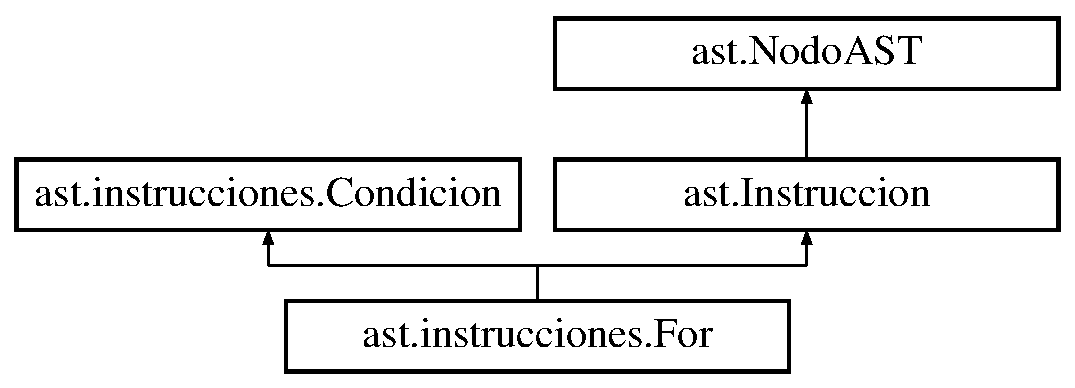
\includegraphics[height=3.000000cm]{classast_1_1instrucciones_1_1_for}
\end{center}
\end{figure}
\subsection*{Public Member Functions}
\begin{DoxyCompactItemize}
\item 
\mbox{\Hypertarget{classast_1_1instrucciones_1_1_for_a8190489ef00a07fdf329f2392878e9e9}\label{classast_1_1instrucciones_1_1_for_a8190489ef00a07fdf329f2392878e9e9}} 
{\bfseries For} (\mbox{\hyperlink{classast_1_1expresiones_1_1_identificador}{Identificador}} id, Linked\+List$<$ \mbox{\hyperlink{interfaceast_1_1_nodo_a_s_t}{Nodo\+A\+ST}} $>$ bloque, \mbox{\hyperlink{interfaceast_1_1_expresion}{Expresion}} cond, int linea, int col)
\item 
\mbox{\Hypertarget{classast_1_1instrucciones_1_1_for_ae8a21c62e52ecdef168ed441ac4775fb}\label{classast_1_1instrucciones_1_1_for_ae8a21c62e52ecdef168ed441ac4775fb}} 
Object {\bfseries ejecutar} (\mbox{\hyperlink{classentorno_1_1_entorno}{Entorno}} ent)
\item 
\mbox{\Hypertarget{classast_1_1instrucciones_1_1_for_a9ed05f6111604bdaa432d0376297d9de}\label{classast_1_1instrucciones_1_1_for_a9ed05f6111604bdaa432d0376297d9de}} 
int {\bfseries linea} ()
\item 
\mbox{\Hypertarget{classast_1_1instrucciones_1_1_for_a16740f86f0eec252fcb4348099be27eb}\label{classast_1_1instrucciones_1_1_for_a16740f86f0eec252fcb4348099be27eb}} 
int {\bfseries columna} ()
\item 
\mbox{\Hypertarget{classast_1_1instrucciones_1_1_for_ac6acbe31ca33914f7041f3b1659dc436}\label{classast_1_1instrucciones_1_1_for_ac6acbe31ca33914f7041f3b1659dc436}} 
String {\bfseries get\+Nombre} (String\+Builder builder, String parent, int cont)
\end{DoxyCompactItemize}


\subsection{Detailed Description}
\begin{DoxyAuthor}{Author}
p\+\_\+ab1 
\end{DoxyAuthor}


The documentation for this class was generated from the following file\+:\begin{DoxyCompactItemize}
\item 
src/ast/instrucciones/For.\+java\end{DoxyCompactItemize}

\hypertarget{classast_1_1instrucciones_1_1funciones_1_1_fstring}{}\section{ast.\+instrucciones.\+funciones.\+Fstring Class Reference}
\label{classast_1_1instrucciones_1_1funciones_1_1_fstring}\index{ast.\+instrucciones.\+funciones.\+Fstring@{ast.\+instrucciones.\+funciones.\+Fstring}}
Inheritance diagram for ast.\+instrucciones.\+funciones.\+Fstring\+:\begin{figure}[H]
\begin{center}
\leavevmode
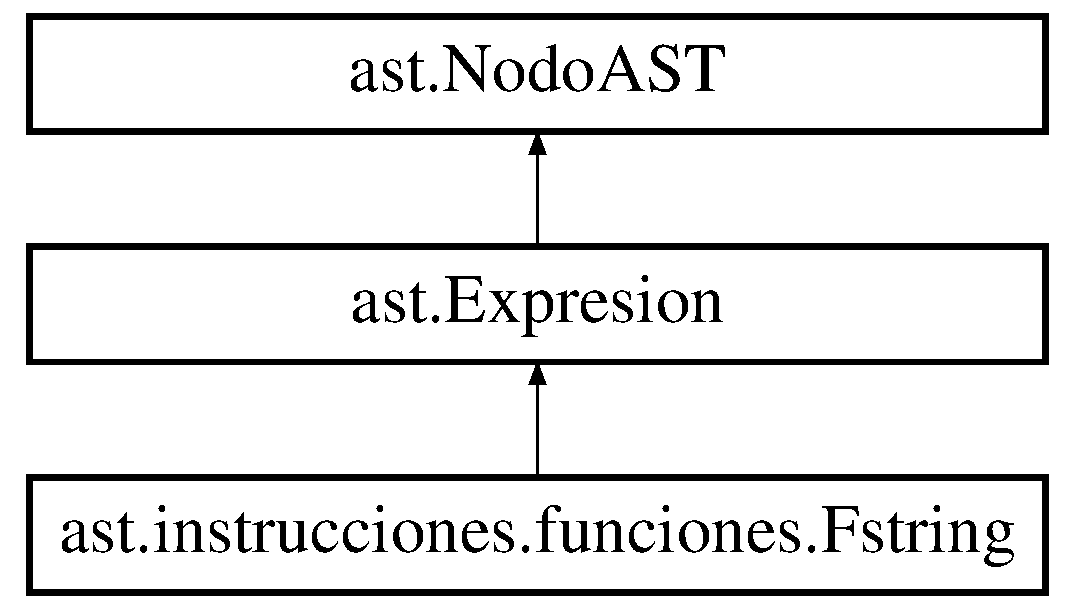
\includegraphics[height=3.000000cm]{classast_1_1instrucciones_1_1funciones_1_1_fstring}
\end{center}
\end{figure}
\subsection*{Public Member Functions}
\begin{DoxyCompactItemize}
\item 
\mbox{\Hypertarget{classast_1_1instrucciones_1_1funciones_1_1_fstring_a72a39df29473431ae389c39e46c68a9f}\label{classast_1_1instrucciones_1_1funciones_1_1_fstring_a72a39df29473431ae389c39e46c68a9f}} 
{\bfseries Fstring} (int tipo, Linked\+List$<$ \mbox{\hyperlink{interfaceast_1_1_nodo_a_s_t}{Nodo\+A\+ST}} $>$ valor, int linea, int col)
\item 
\mbox{\Hypertarget{classast_1_1instrucciones_1_1funciones_1_1_fstring_ab82a7413094cc0f7cfd2fee6154dfc32}\label{classast_1_1instrucciones_1_1funciones_1_1_fstring_ab82a7413094cc0f7cfd2fee6154dfc32}} 
\mbox{\hyperlink{classentorno_1_1_tipo}{Tipo}} {\bfseries get\+Tipo} (\mbox{\hyperlink{classentorno_1_1_entorno}{Entorno}} ent)
\item 
\mbox{\Hypertarget{classast_1_1instrucciones_1_1funciones_1_1_fstring_af0ff90be18a90396c724e48e9181d7bf}\label{classast_1_1instrucciones_1_1funciones_1_1_fstring_af0ff90be18a90396c724e48e9181d7bf}} 
Object {\bfseries get\+Valor\+Implicito} (\mbox{\hyperlink{classentorno_1_1_entorno}{Entorno}} ent)
\item 
\mbox{\Hypertarget{classast_1_1instrucciones_1_1funciones_1_1_fstring_a36d5b53a469376042f07960c110fd1f0}\label{classast_1_1instrucciones_1_1funciones_1_1_fstring_a36d5b53a469376042f07960c110fd1f0}} 
int {\bfseries linea} ()
\item 
\mbox{\Hypertarget{classast_1_1instrucciones_1_1funciones_1_1_fstring_ae9316037ad4f53e4fcfbe36446473ee7}\label{classast_1_1instrucciones_1_1funciones_1_1_fstring_ae9316037ad4f53e4fcfbe36446473ee7}} 
int {\bfseries columna} ()
\item 
\mbox{\Hypertarget{classast_1_1instrucciones_1_1funciones_1_1_fstring_a0239f774aa2f7b262bcc4bcf3a636f73}\label{classast_1_1instrucciones_1_1funciones_1_1_fstring_a0239f774aa2f7b262bcc4bcf3a636f73}} 
String {\bfseries get\+Nombre} (String\+Builder builder, String parent, int cont)
\end{DoxyCompactItemize}


\subsection{Detailed Description}
\begin{DoxyAuthor}{Author}
p\+\_\+ab1 
\end{DoxyAuthor}


The documentation for this class was generated from the following file\+:\begin{DoxyCompactItemize}
\item 
src/ast/instrucciones/funciones/Fstring.\+java\end{DoxyCompactItemize}

\hypertarget{classast_1_1instrucciones_1_1_funcion}{}\section{ast.\+instrucciones.\+Funcion Class Reference}
\label{classast_1_1instrucciones_1_1_funcion}\index{ast.\+instrucciones.\+Funcion@{ast.\+instrucciones.\+Funcion}}
Inheritance diagram for ast.\+instrucciones.\+Funcion\+:\begin{figure}[H]
\begin{center}
\leavevmode
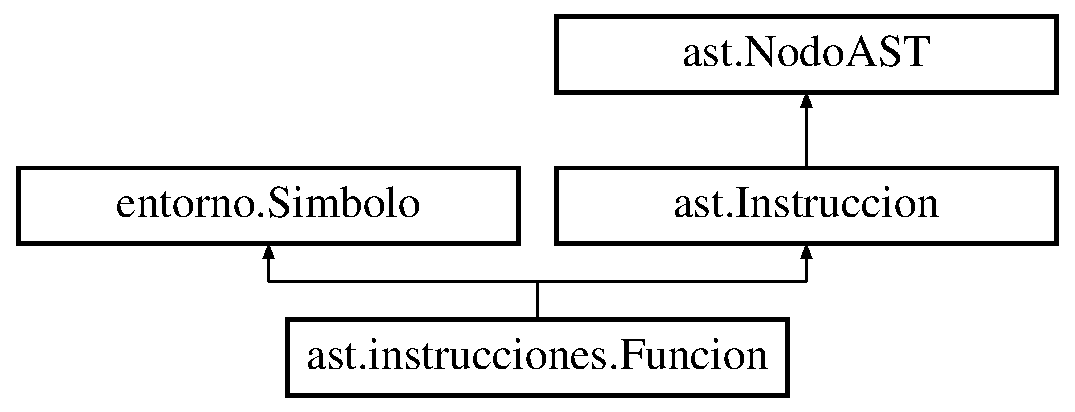
\includegraphics[height=3.000000cm]{classast_1_1instrucciones_1_1_funcion}
\end{center}
\end{figure}
\subsection*{Public Member Functions}
\begin{DoxyCompactItemize}
\item 
\mbox{\Hypertarget{classast_1_1instrucciones_1_1_funcion_aaabae2fd7dbd2317571610df212f4ec7}\label{classast_1_1instrucciones_1_1_funcion_aaabae2fd7dbd2317571610df212f4ec7}} 
{\bfseries Funcion} (String id, \mbox{\hyperlink{enumentorno_1_1_simbolo_1_1_rol}{Rol}} rol, Linked\+List$<$ \mbox{\hyperlink{classentorno_1_1_simbolo}{Simbolo}} $>$ parametros\+Formales, Linked\+List$<$ \mbox{\hyperlink{interfaceast_1_1_nodo_a_s_t}{Nodo\+A\+ST}} $>$ sentencias, int linea, int col)
\item 
\mbox{\Hypertarget{classast_1_1instrucciones_1_1_funcion_ac3d6c8fe5070514662aabcc485032fba}\label{classast_1_1instrucciones_1_1_funcion_ac3d6c8fe5070514662aabcc485032fba}} 
{\bfseries Funcion} (String id, \mbox{\hyperlink{enumentorno_1_1_simbolo_1_1_rol}{Rol}} rol, Linked\+List$<$ \mbox{\hyperlink{interfaceast_1_1_nodo_a_s_t}{Nodo\+A\+ST}} $>$ sentencias, int linea, int col)
\item 
\mbox{\Hypertarget{classast_1_1instrucciones_1_1_funcion_a0097f4cae30c3e065ed15282fc851b0a}\label{classast_1_1instrucciones_1_1_funcion_a0097f4cae30c3e065ed15282fc851b0a}} 
void {\bfseries set\+Identificador} (String identificador)
\item 
\mbox{\Hypertarget{classast_1_1instrucciones_1_1_funcion_a5861f1d779a87d0ac72deee25602b044}\label{classast_1_1instrucciones_1_1_funcion_a5861f1d779a87d0ac72deee25602b044}} 
Object {\bfseries ejecutar} (\mbox{\hyperlink{classentorno_1_1_entorno}{Entorno}} ent)
\item 
\mbox{\Hypertarget{classast_1_1instrucciones_1_1_funcion_ada9350b49520c6c411d4479a08b90655}\label{classast_1_1instrucciones_1_1_funcion_ada9350b49520c6c411d4479a08b90655}} 
int {\bfseries linea} ()
\item 
\mbox{\Hypertarget{classast_1_1instrucciones_1_1_funcion_ab0aa9a20dcc240ec952556da7a3833f1}\label{classast_1_1instrucciones_1_1_funcion_ab0aa9a20dcc240ec952556da7a3833f1}} 
Linked\+List$<$ \mbox{\hyperlink{classentorno_1_1_simbolo}{Simbolo}} $>$ {\bfseries get\+Parametros\+Formales} ()
\item 
\mbox{\Hypertarget{classast_1_1instrucciones_1_1_funcion_a5ec7cbf4247459103a21d547a0980635}\label{classast_1_1instrucciones_1_1_funcion_a5ec7cbf4247459103a21d547a0980635}} 
void {\bfseries set\+Parametros\+Formales} (Linked\+List$<$ \mbox{\hyperlink{classentorno_1_1_simbolo}{Simbolo}} $>$ parametros\+Formales)
\item 
\mbox{\Hypertarget{classast_1_1instrucciones_1_1_funcion_a5d69ae86434636e40863d566e8e5907f}\label{classast_1_1instrucciones_1_1_funcion_a5d69ae86434636e40863d566e8e5907f}} 
Linked\+List$<$ \mbox{\hyperlink{interfaceast_1_1_nodo_a_s_t}{Nodo\+A\+ST}} $>$ {\bfseries get\+Sentencias} ()
\item 
\mbox{\Hypertarget{classast_1_1instrucciones_1_1_funcion_a2971bfe4d6d7372d38789b3264c72cf8}\label{classast_1_1instrucciones_1_1_funcion_a2971bfe4d6d7372d38789b3264c72cf8}} 
void {\bfseries set\+Sentencias} (Linked\+List$<$ \mbox{\hyperlink{interfaceast_1_1_nodo_a_s_t}{Nodo\+A\+ST}} $>$ sentencias)
\item 
\mbox{\Hypertarget{classast_1_1instrucciones_1_1_funcion_a66334c8bf95e6791cfaca7c1731ec11c}\label{classast_1_1instrucciones_1_1_funcion_a66334c8bf95e6791cfaca7c1731ec11c}} 
int {\bfseries columna} ()
\item 
\mbox{\Hypertarget{classast_1_1instrucciones_1_1_funcion_aaf67056d3d4c959ee09d1cee4e145a03}\label{classast_1_1instrucciones_1_1_funcion_aaf67056d3d4c959ee09d1cee4e145a03}} 
String {\bfseries get\+Nombre} (String\+Builder builder, String parent, int cont)
\end{DoxyCompactItemize}
\subsection*{Additional Inherited Members}


\subsection{Detailed Description}
\begin{DoxyAuthor}{Author}
p\+\_\+ab1 
\end{DoxyAuthor}


The documentation for this class was generated from the following file\+:\begin{DoxyCompactItemize}
\item 
src/ast/instrucciones/Funcion.\+java\end{DoxyCompactItemize}

\hypertarget{classast_1_1instrucciones_1_1funciones_1_1funcion_c}{}\section{ast.\+instrucciones.\+funciones.\+funcionC Class Reference}
\label{classast_1_1instrucciones_1_1funciones_1_1funcion_c}\index{ast.\+instrucciones.\+funciones.\+funcionC@{ast.\+instrucciones.\+funciones.\+funcionC}}
Inheritance diagram for ast.\+instrucciones.\+funciones.\+funcionC\+:\begin{figure}[H]
\begin{center}
\leavevmode
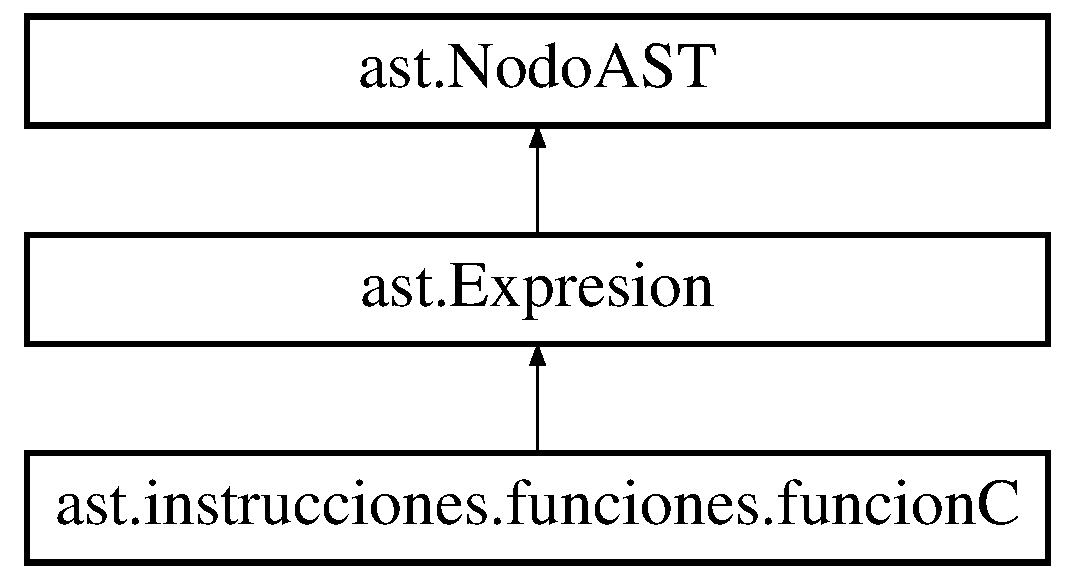
\includegraphics[height=3.000000cm]{classast_1_1instrucciones_1_1funciones_1_1funcion_c}
\end{center}
\end{figure}
\subsection*{Public Member Functions}
\begin{DoxyCompactItemize}
\item 
\mbox{\Hypertarget{classast_1_1instrucciones_1_1funciones_1_1funcion_c_af93ed562ec886978d49870d7270ef78a}\label{classast_1_1instrucciones_1_1funciones_1_1funcion_c_af93ed562ec886978d49870d7270ef78a}} 
{\bfseries funcionC} (Linked\+List$<$ \mbox{\hyperlink{interfaceast_1_1_nodo_a_s_t}{Nodo\+A\+ST}} $>$ lista\+Exp, int linea, int col)
\item 
\mbox{\Hypertarget{classast_1_1instrucciones_1_1funciones_1_1funcion_c_a32954fba31baaa1692ec25d40b6c39a3}\label{classast_1_1instrucciones_1_1funciones_1_1funcion_c_a32954fba31baaa1692ec25d40b6c39a3}} 
\mbox{\hyperlink{classentorno_1_1_tipo}{Tipo}} {\bfseries get\+Tipo} (\mbox{\hyperlink{classentorno_1_1_entorno}{Entorno}} ent)
\item 
\mbox{\Hypertarget{classast_1_1instrucciones_1_1funciones_1_1funcion_c_af28116d5f1891f909fa514e912378cd1}\label{classast_1_1instrucciones_1_1funciones_1_1funcion_c_af28116d5f1891f909fa514e912378cd1}} 
Object {\bfseries get\+Valor\+Implicito} (\mbox{\hyperlink{classentorno_1_1_entorno}{Entorno}} ent)
\item 
\mbox{\Hypertarget{classast_1_1instrucciones_1_1funciones_1_1funcion_c_a9755ba403d4f39c9115bddfca8296fa7}\label{classast_1_1instrucciones_1_1funciones_1_1funcion_c_a9755ba403d4f39c9115bddfca8296fa7}} 
int {\bfseries linea} ()
\item 
\mbox{\Hypertarget{classast_1_1instrucciones_1_1funciones_1_1funcion_c_a2f55b1386af476c0199472db95c5fd5a}\label{classast_1_1instrucciones_1_1funciones_1_1funcion_c_a2f55b1386af476c0199472db95c5fd5a}} 
int {\bfseries columna} ()
\item 
\mbox{\Hypertarget{classast_1_1instrucciones_1_1funciones_1_1funcion_c_aecf9833f34a1a9dec50dc3e09f6ff79e}\label{classast_1_1instrucciones_1_1funciones_1_1funcion_c_aecf9833f34a1a9dec50dc3e09f6ff79e}} 
String {\bfseries get\+Nombre} (String\+Builder builder, String parent, int cont)
\end{DoxyCompactItemize}


\subsection{Detailed Description}
\begin{DoxyAuthor}{Author}
p\+\_\+ab1 
\end{DoxyAuthor}


The documentation for this class was generated from the following file\+:\begin{DoxyCompactItemize}
\item 
src/ast/instrucciones/funciones/funcion\+C.\+java\end{DoxyCompactItemize}

\hypertarget{classast_1_1instrucciones_1_1funciones_1_1_funcion_matrix}{}\section{ast.\+instrucciones.\+funciones.\+Funcion\+Matrix Class Reference}
\label{classast_1_1instrucciones_1_1funciones_1_1_funcion_matrix}\index{ast.\+instrucciones.\+funciones.\+Funcion\+Matrix@{ast.\+instrucciones.\+funciones.\+Funcion\+Matrix}}
Inheritance diagram for ast.\+instrucciones.\+funciones.\+Funcion\+Matrix\+:\begin{figure}[H]
\begin{center}
\leavevmode
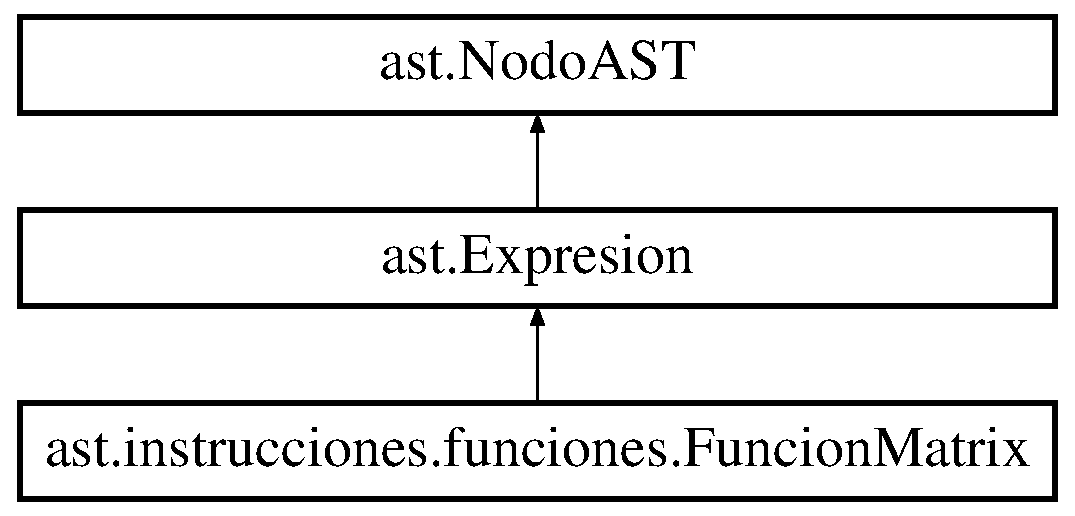
\includegraphics[height=3.000000cm]{classast_1_1instrucciones_1_1funciones_1_1_funcion_matrix}
\end{center}
\end{figure}
\subsection*{Public Member Functions}
\begin{DoxyCompactItemize}
\item 
\mbox{\Hypertarget{classast_1_1instrucciones_1_1funciones_1_1_funcion_matrix_a9607ad469eb52695322450a2ce4fbd9a}\label{classast_1_1instrucciones_1_1funciones_1_1_funcion_matrix_a9607ad469eb52695322450a2ce4fbd9a}} 
{\bfseries Funcion\+Matrix} (Linked\+List$<$ \mbox{\hyperlink{interfaceast_1_1_nodo_a_s_t}{Nodo\+A\+ST}} $>$ lista\+Exp, int linea, int col)
\item 
\mbox{\Hypertarget{classast_1_1instrucciones_1_1funciones_1_1_funcion_matrix_ac97af3af5a2efa36a97433fc7333e5e0}\label{classast_1_1instrucciones_1_1funciones_1_1_funcion_matrix_ac97af3af5a2efa36a97433fc7333e5e0}} 
\mbox{\hyperlink{classentorno_1_1_tipo}{Tipo}} {\bfseries get\+Tipo} (\mbox{\hyperlink{classentorno_1_1_entorno}{Entorno}} ent)
\item 
\mbox{\Hypertarget{classast_1_1instrucciones_1_1funciones_1_1_funcion_matrix_a59e1e6f1d5fb6cbce7d2f337a8cc23df}\label{classast_1_1instrucciones_1_1funciones_1_1_funcion_matrix_a59e1e6f1d5fb6cbce7d2f337a8cc23df}} 
Object {\bfseries get\+Valor\+Implicito} (\mbox{\hyperlink{classentorno_1_1_entorno}{Entorno}} ent)
\item 
\mbox{\Hypertarget{classast_1_1instrucciones_1_1funciones_1_1_funcion_matrix_ada402920e5404210f498dd5f8a43c32d}\label{classast_1_1instrucciones_1_1funciones_1_1_funcion_matrix_ada402920e5404210f498dd5f8a43c32d}} 
int {\bfseries linea} ()
\item 
\mbox{\Hypertarget{classast_1_1instrucciones_1_1funciones_1_1_funcion_matrix_a42e623f3e0289b04c2383d2a35b06a6b}\label{classast_1_1instrucciones_1_1funciones_1_1_funcion_matrix_a42e623f3e0289b04c2383d2a35b06a6b}} 
int {\bfseries columna} ()
\item 
\mbox{\Hypertarget{classast_1_1instrucciones_1_1funciones_1_1_funcion_matrix_addd2b583e2cbe14c8b1d7f578dd6ae31}\label{classast_1_1instrucciones_1_1funciones_1_1_funcion_matrix_addd2b583e2cbe14c8b1d7f578dd6ae31}} 
String {\bfseries get\+Nombre} (String\+Builder builder, String parent, int cont)
\end{DoxyCompactItemize}
\subsection*{Static Public Member Functions}
\begin{DoxyCompactItemize}
\item 
\mbox{\Hypertarget{classast_1_1instrucciones_1_1funciones_1_1_funcion_matrix_a648bcda532036979d24215c3b7b4bdd4}\label{classast_1_1instrucciones_1_1funciones_1_1_funcion_matrix_a648bcda532036979d24215c3b7b4bdd4}} 
static Object {\bfseries get\+Valores\+Matriz} (\mbox{\hyperlink{classentorno_1_1nodo_exp}{nodo\+Exp}} e, Object\mbox{[}$\,$\mbox{]}\mbox{[}$\,$\mbox{]} mat, \mbox{\hyperlink{classentorno_1_1_entorno}{Entorno}} ent)
\end{DoxyCompactItemize}


\subsection{Detailed Description}
\begin{DoxyAuthor}{Author}
hp 
\end{DoxyAuthor}


The documentation for this class was generated from the following file\+:\begin{DoxyCompactItemize}
\item 
src/ast/instrucciones/funciones/Funcion\+Matrix.\+java\end{DoxyCompactItemize}

\hypertarget{classast_1_1instrucciones_1_1funciones_1_1_generar_list}{}\section{ast.\+instrucciones.\+funciones.\+Generar\+List Class Reference}
\label{classast_1_1instrucciones_1_1funciones_1_1_generar_list}\index{ast.\+instrucciones.\+funciones.\+Generar\+List@{ast.\+instrucciones.\+funciones.\+Generar\+List}}
Inheritance diagram for ast.\+instrucciones.\+funciones.\+Generar\+List\+:\begin{figure}[H]
\begin{center}
\leavevmode
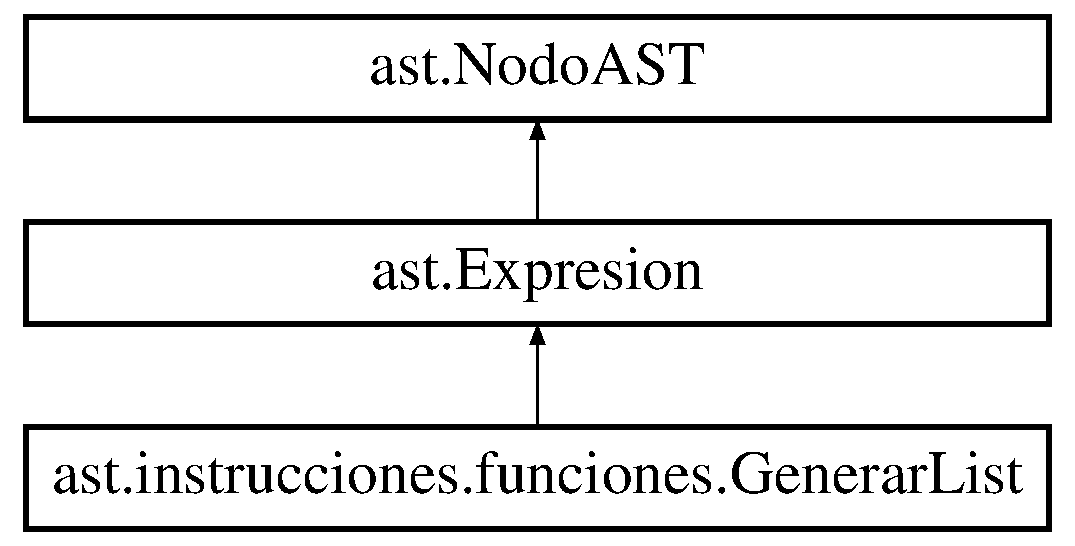
\includegraphics[height=3.000000cm]{classast_1_1instrucciones_1_1funciones_1_1_generar_list}
\end{center}
\end{figure}
\subsection*{Public Member Functions}
\begin{DoxyCompactItemize}
\item 
\mbox{\Hypertarget{classast_1_1instrucciones_1_1funciones_1_1_generar_list_ae997ea30656501e2a1b205b6227dc782}\label{classast_1_1instrucciones_1_1funciones_1_1_generar_list_ae997ea30656501e2a1b205b6227dc782}} 
{\bfseries Generar\+List} (Linked\+List$<$ \mbox{\hyperlink{interfaceast_1_1_nodo_a_s_t}{Nodo\+A\+ST}} $>$ lista\+Exp, int linea, int col)
\item 
\mbox{\Hypertarget{classast_1_1instrucciones_1_1funciones_1_1_generar_list_a547699bf27970547f341f3c30334a583}\label{classast_1_1instrucciones_1_1funciones_1_1_generar_list_a547699bf27970547f341f3c30334a583}} 
\mbox{\hyperlink{classentorno_1_1_tipo}{Tipo}} {\bfseries get\+Tipo} (\mbox{\hyperlink{classentorno_1_1_entorno}{Entorno}} ent)
\item 
\mbox{\Hypertarget{classast_1_1instrucciones_1_1funciones_1_1_generar_list_a1da1f232c40ab3edeac73969bfe994ab}\label{classast_1_1instrucciones_1_1funciones_1_1_generar_list_a1da1f232c40ab3edeac73969bfe994ab}} 
Object {\bfseries get\+Valor\+Implicito} (\mbox{\hyperlink{classentorno_1_1_entorno}{Entorno}} ent)
\item 
\mbox{\Hypertarget{classast_1_1instrucciones_1_1funciones_1_1_generar_list_a92a1069f5a1097b9ad69ea2db2e3354e}\label{classast_1_1instrucciones_1_1funciones_1_1_generar_list_a92a1069f5a1097b9ad69ea2db2e3354e}} 
int {\bfseries linea} ()
\item 
\mbox{\Hypertarget{classast_1_1instrucciones_1_1funciones_1_1_generar_list_a5ef87128e259b0b14a9d7ea86160a4ad}\label{classast_1_1instrucciones_1_1funciones_1_1_generar_list_a5ef87128e259b0b14a9d7ea86160a4ad}} 
int {\bfseries columna} ()
\item 
\mbox{\Hypertarget{classast_1_1instrucciones_1_1funciones_1_1_generar_list_aae08f004aa5c87dd72345c4e6d403f94}\label{classast_1_1instrucciones_1_1funciones_1_1_generar_list_aae08f004aa5c87dd72345c4e6d403f94}} 
String {\bfseries get\+Nombre} (String\+Builder builder, String parent, int cont)
\end{DoxyCompactItemize}


\subsection{Detailed Description}
\begin{DoxyAuthor}{Author}
p\+\_\+ab1 
\end{DoxyAuthor}


The documentation for this class was generated from the following file\+:\begin{DoxyCompactItemize}
\item 
src/ast/instrucciones/funciones/Generar\+List.\+java\end{DoxyCompactItemize}

\hypertarget{classast_1_1instrucciones_1_1graficas_1_1graf_barras}{}\section{ast.\+instrucciones.\+graficas.\+graf\+Barras Class Reference}
\label{classast_1_1instrucciones_1_1graficas_1_1graf_barras}\index{ast.\+instrucciones.\+graficas.\+graf\+Barras@{ast.\+instrucciones.\+graficas.\+graf\+Barras}}
Inheritance diagram for ast.\+instrucciones.\+graficas.\+graf\+Barras\+:\begin{figure}[H]
\begin{center}
\leavevmode
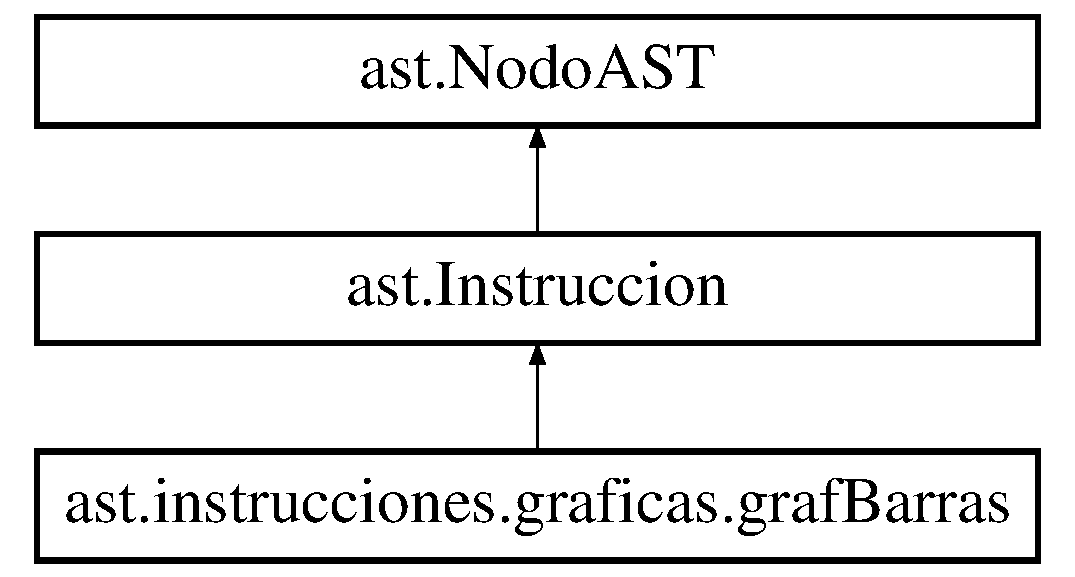
\includegraphics[height=3.000000cm]{classast_1_1instrucciones_1_1graficas_1_1graf_barras}
\end{center}
\end{figure}
\subsection*{Public Member Functions}
\begin{DoxyCompactItemize}
\item 
\mbox{\Hypertarget{classast_1_1instrucciones_1_1graficas_1_1graf_barras_a730997c92ff80c5e0ec73620b1d14a2b}\label{classast_1_1instrucciones_1_1graficas_1_1graf_barras_a730997c92ff80c5e0ec73620b1d14a2b}} 
{\bfseries graf\+Barras} (Linked\+List$<$ \mbox{\hyperlink{interfaceast_1_1_nodo_a_s_t}{Nodo\+A\+ST}} $>$ lista, int linea, int col)
\item 
\mbox{\Hypertarget{classast_1_1instrucciones_1_1graficas_1_1graf_barras_af9faa1a9539984ead67f4bbfe79e5c84}\label{classast_1_1instrucciones_1_1graficas_1_1graf_barras_af9faa1a9539984ead67f4bbfe79e5c84}} 
Object {\bfseries ejecutar} (\mbox{\hyperlink{classentorno_1_1_entorno}{Entorno}} ent)
\item 
\mbox{\Hypertarget{classast_1_1instrucciones_1_1graficas_1_1graf_barras_a174231deff52a178e12a49f3120b89d6}\label{classast_1_1instrucciones_1_1graficas_1_1graf_barras_a174231deff52a178e12a49f3120b89d6}} 
int {\bfseries linea} ()
\item 
\mbox{\Hypertarget{classast_1_1instrucciones_1_1graficas_1_1graf_barras_aad96a2b643fdd6f1fe83260b5a8e872b}\label{classast_1_1instrucciones_1_1graficas_1_1graf_barras_aad96a2b643fdd6f1fe83260b5a8e872b}} 
int {\bfseries columna} ()
\item 
\mbox{\Hypertarget{classast_1_1instrucciones_1_1graficas_1_1graf_barras_a6c9af2a57ad2fb50dce2eae3365715e0}\label{classast_1_1instrucciones_1_1graficas_1_1graf_barras_a6c9af2a57ad2fb50dce2eae3365715e0}} 
String {\bfseries get\+Nombre} (String\+Builder builder, String parent, int cont)
\end{DoxyCompactItemize}


\subsection{Detailed Description}
\begin{DoxyAuthor}{Author}
p\+\_\+ab1 
\end{DoxyAuthor}


The documentation for this class was generated from the following file\+:\begin{DoxyCompactItemize}
\item 
src/ast/instrucciones/graficas/graf\+Barras.\+java\end{DoxyCompactItemize}

\hypertarget{classast_1_1instrucciones_1_1graficas_1_1graf_dispersion}{}\section{ast.\+instrucciones.\+graficas.\+graf\+Dispersion Class Reference}
\label{classast_1_1instrucciones_1_1graficas_1_1graf_dispersion}\index{ast.\+instrucciones.\+graficas.\+graf\+Dispersion@{ast.\+instrucciones.\+graficas.\+graf\+Dispersion}}
Inheritance diagram for ast.\+instrucciones.\+graficas.\+graf\+Dispersion\+:\begin{figure}[H]
\begin{center}
\leavevmode
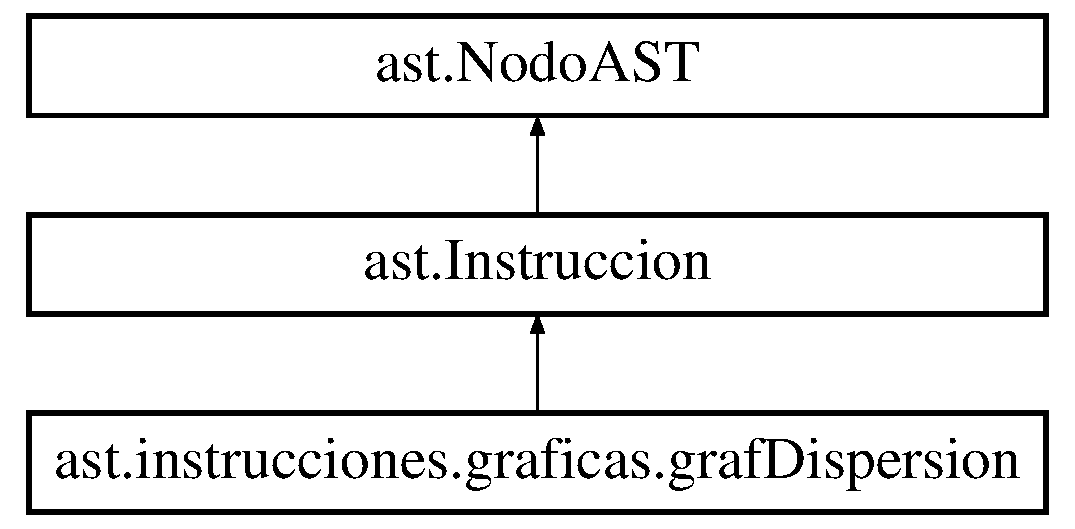
\includegraphics[height=3.000000cm]{classast_1_1instrucciones_1_1graficas_1_1graf_dispersion}
\end{center}
\end{figure}
\subsection*{Public Member Functions}
\begin{DoxyCompactItemize}
\item 
\mbox{\Hypertarget{classast_1_1instrucciones_1_1graficas_1_1graf_dispersion_ac66ae765e6a5140a669c7216c2d61759}\label{classast_1_1instrucciones_1_1graficas_1_1graf_dispersion_ac66ae765e6a5140a669c7216c2d61759}} 
{\bfseries graf\+Dispersion} (Linked\+List$<$ \mbox{\hyperlink{interfaceast_1_1_nodo_a_s_t}{Nodo\+A\+ST}} $>$ lista, int linea, int col)
\item 
\mbox{\Hypertarget{classast_1_1instrucciones_1_1graficas_1_1graf_dispersion_a8926d9b2844b4bcfe0966e1e89cc0fa6}\label{classast_1_1instrucciones_1_1graficas_1_1graf_dispersion_a8926d9b2844b4bcfe0966e1e89cc0fa6}} 
Object {\bfseries ejecutar} (\mbox{\hyperlink{classentorno_1_1_entorno}{Entorno}} ent)
\item 
\mbox{\Hypertarget{classast_1_1instrucciones_1_1graficas_1_1graf_dispersion_a5a1cb628350719206704f21a8ea438e3}\label{classast_1_1instrucciones_1_1graficas_1_1graf_dispersion_a5a1cb628350719206704f21a8ea438e3}} 
int {\bfseries linea} ()
\item 
\mbox{\Hypertarget{classast_1_1instrucciones_1_1graficas_1_1graf_dispersion_afc9d93242c8b1371ee6d6286723121fe}\label{classast_1_1instrucciones_1_1graficas_1_1graf_dispersion_afc9d93242c8b1371ee6d6286723121fe}} 
int {\bfseries columna} ()
\item 
\mbox{\Hypertarget{classast_1_1instrucciones_1_1graficas_1_1graf_dispersion_ab0590544f132a3a7717e797d2d675a61}\label{classast_1_1instrucciones_1_1graficas_1_1graf_dispersion_ab0590544f132a3a7717e797d2d675a61}} 
String {\bfseries get\+Nombre} (String\+Builder builder, String parent, int cont)
\end{DoxyCompactItemize}


\subsection{Detailed Description}
\begin{DoxyAuthor}{Author}
p\+\_\+ab1 
\end{DoxyAuthor}


The documentation for this class was generated from the following file\+:\begin{DoxyCompactItemize}
\item 
src/ast/instrucciones/graficas/graf\+Dispersion.\+java\end{DoxyCompactItemize}

\hypertarget{classast_1_1instrucciones_1_1graficas_1_1graf_histograma}{}\section{ast.\+instrucciones.\+graficas.\+graf\+Histograma Class Reference}
\label{classast_1_1instrucciones_1_1graficas_1_1graf_histograma}\index{ast.\+instrucciones.\+graficas.\+graf\+Histograma@{ast.\+instrucciones.\+graficas.\+graf\+Histograma}}
Inheritance diagram for ast.\+instrucciones.\+graficas.\+graf\+Histograma\+:\begin{figure}[H]
\begin{center}
\leavevmode
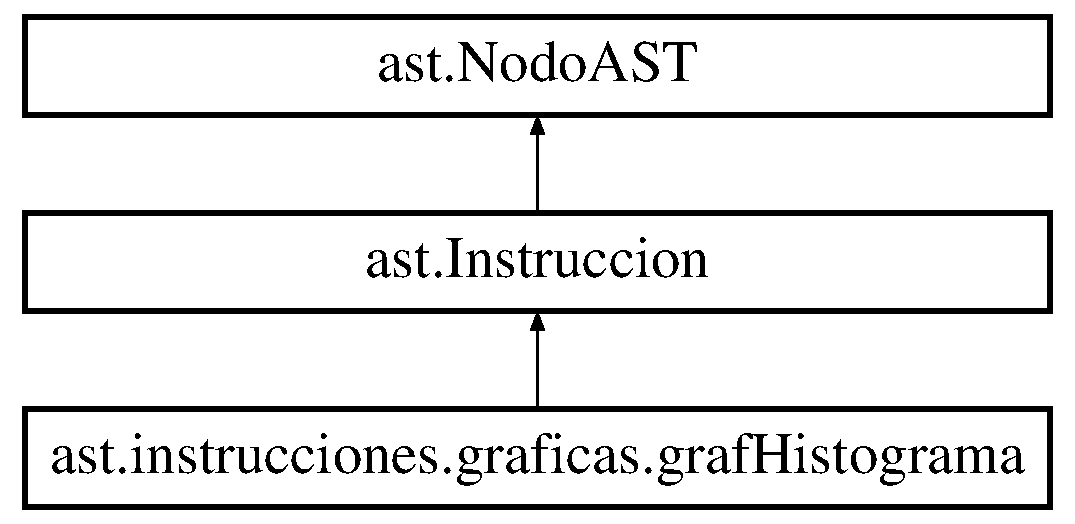
\includegraphics[height=3.000000cm]{classast_1_1instrucciones_1_1graficas_1_1graf_histograma}
\end{center}
\end{figure}
\subsection*{Public Member Functions}
\begin{DoxyCompactItemize}
\item 
\mbox{\Hypertarget{classast_1_1instrucciones_1_1graficas_1_1graf_histograma_a1dc9fead227728978dd651250d612ee6}\label{classast_1_1instrucciones_1_1graficas_1_1graf_histograma_a1dc9fead227728978dd651250d612ee6}} 
{\bfseries graf\+Histograma} (Linked\+List$<$ \mbox{\hyperlink{interfaceast_1_1_nodo_a_s_t}{Nodo\+A\+ST}} $>$ lista, int linea, int col)
\item 
\mbox{\Hypertarget{classast_1_1instrucciones_1_1graficas_1_1graf_histograma_aa90322ce25d7c052b64df2c67dee9be8}\label{classast_1_1instrucciones_1_1graficas_1_1graf_histograma_aa90322ce25d7c052b64df2c67dee9be8}} 
Object {\bfseries ejecutar} (\mbox{\hyperlink{classentorno_1_1_entorno}{Entorno}} ent)
\item 
\mbox{\Hypertarget{classast_1_1instrucciones_1_1graficas_1_1graf_histograma_a88b559e820cb76ec36734cbf982fefba}\label{classast_1_1instrucciones_1_1graficas_1_1graf_histograma_a88b559e820cb76ec36734cbf982fefba}} 
int {\bfseries linea} ()
\item 
\mbox{\Hypertarget{classast_1_1instrucciones_1_1graficas_1_1graf_histograma_a79ac6464c124223eb53b2233a041415b}\label{classast_1_1instrucciones_1_1graficas_1_1graf_histograma_a79ac6464c124223eb53b2233a041415b}} 
int {\bfseries columna} ()
\item 
\mbox{\Hypertarget{classast_1_1instrucciones_1_1graficas_1_1graf_histograma_a9138e575238f4a165f1531e0341c4e6e}\label{classast_1_1instrucciones_1_1graficas_1_1graf_histograma_a9138e575238f4a165f1531e0341c4e6e}} 
String {\bfseries get\+Nombre} (String\+Builder builder, String parent, int cont)
\end{DoxyCompactItemize}


\subsection{Detailed Description}
\begin{DoxyAuthor}{Author}
p\+\_\+ab1 
\end{DoxyAuthor}


The documentation for this class was generated from the following file\+:\begin{DoxyCompactItemize}
\item 
src/ast/instrucciones/graficas/graf\+Histograma.\+java\end{DoxyCompactItemize}

\hypertarget{classast_1_1instrucciones_1_1graficas_1_1graf_lineas}{}\section{ast.\+instrucciones.\+graficas.\+graf\+Lineas Class Reference}
\label{classast_1_1instrucciones_1_1graficas_1_1graf_lineas}\index{ast.\+instrucciones.\+graficas.\+graf\+Lineas@{ast.\+instrucciones.\+graficas.\+graf\+Lineas}}
Inheritance diagram for ast.\+instrucciones.\+graficas.\+graf\+Lineas\+:\begin{figure}[H]
\begin{center}
\leavevmode
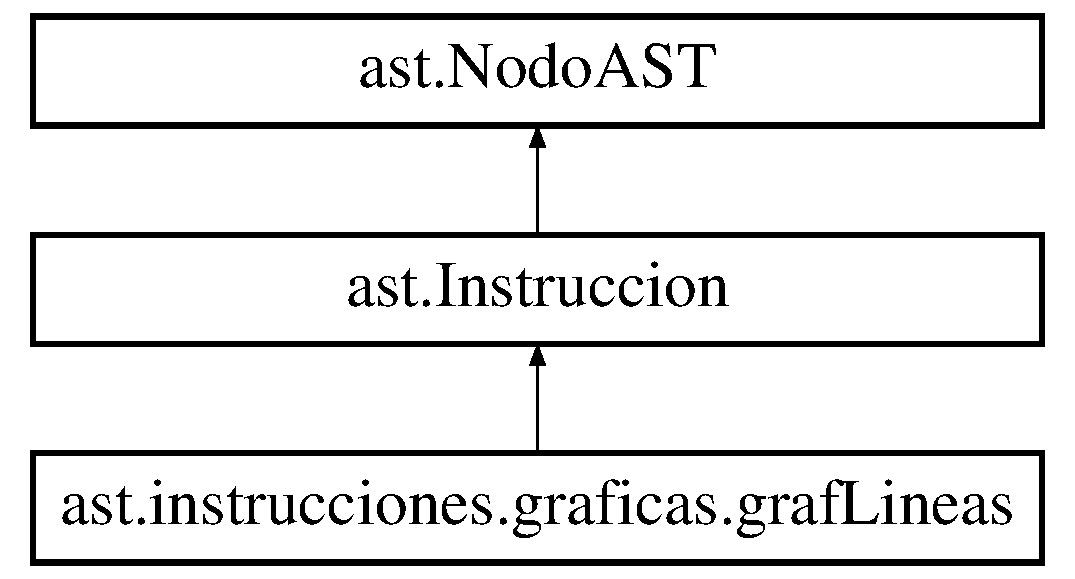
\includegraphics[height=3.000000cm]{classast_1_1instrucciones_1_1graficas_1_1graf_lineas}
\end{center}
\end{figure}
\subsection*{Public Member Functions}
\begin{DoxyCompactItemize}
\item 
\mbox{\Hypertarget{classast_1_1instrucciones_1_1graficas_1_1graf_lineas_a14ab6b521856c0c935c3a57dff020936}\label{classast_1_1instrucciones_1_1graficas_1_1graf_lineas_a14ab6b521856c0c935c3a57dff020936}} 
{\bfseries graf\+Lineas} (Linked\+List$<$ \mbox{\hyperlink{interfaceast_1_1_nodo_a_s_t}{Nodo\+A\+ST}} $>$ lista, int linea, int col)
\item 
\mbox{\Hypertarget{classast_1_1instrucciones_1_1graficas_1_1graf_lineas_aa76cb98a3757b5df941f0220c8f97be9}\label{classast_1_1instrucciones_1_1graficas_1_1graf_lineas_aa76cb98a3757b5df941f0220c8f97be9}} 
Object {\bfseries ejecutar} (\mbox{\hyperlink{classentorno_1_1_entorno}{Entorno}} ent)
\item 
\mbox{\Hypertarget{classast_1_1instrucciones_1_1graficas_1_1graf_lineas_a367d82b82ab29725a6b1df12a089f4f9}\label{classast_1_1instrucciones_1_1graficas_1_1graf_lineas_a367d82b82ab29725a6b1df12a089f4f9}} 
int {\bfseries linea} ()
\item 
\mbox{\Hypertarget{classast_1_1instrucciones_1_1graficas_1_1graf_lineas_a8250ad820ec851d559cf4c93f67cd6e9}\label{classast_1_1instrucciones_1_1graficas_1_1graf_lineas_a8250ad820ec851d559cf4c93f67cd6e9}} 
int {\bfseries columna} ()
\item 
\mbox{\Hypertarget{classast_1_1instrucciones_1_1graficas_1_1graf_lineas_a4c4f727dee1fd573d1c6d7f9043f9926}\label{classast_1_1instrucciones_1_1graficas_1_1graf_lineas_a4c4f727dee1fd573d1c6d7f9043f9926}} 
String {\bfseries get\+Nombre} (String\+Builder builder, String parent, int cont)
\end{DoxyCompactItemize}


\subsection{Detailed Description}
\begin{DoxyAuthor}{Author}
p\+\_\+ab1 
\end{DoxyAuthor}


The documentation for this class was generated from the following file\+:\begin{DoxyCompactItemize}
\item 
src/ast/instrucciones/graficas/graf\+Lineas.\+java\end{DoxyCompactItemize}

\hypertarget{classast_1_1instrucciones_1_1graficas_1_1graf_pie}{}\section{ast.\+instrucciones.\+graficas.\+graf\+Pie Class Reference}
\label{classast_1_1instrucciones_1_1graficas_1_1graf_pie}\index{ast.\+instrucciones.\+graficas.\+graf\+Pie@{ast.\+instrucciones.\+graficas.\+graf\+Pie}}
Inheritance diagram for ast.\+instrucciones.\+graficas.\+graf\+Pie\+:\begin{figure}[H]
\begin{center}
\leavevmode
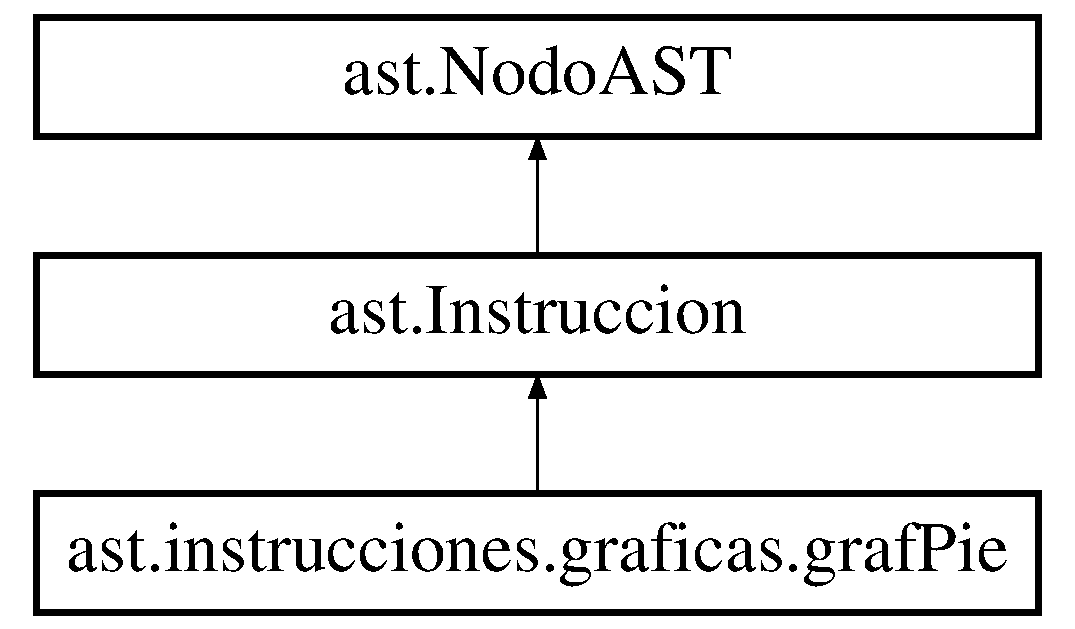
\includegraphics[height=3.000000cm]{classast_1_1instrucciones_1_1graficas_1_1graf_pie}
\end{center}
\end{figure}
\subsection*{Public Member Functions}
\begin{DoxyCompactItemize}
\item 
\mbox{\Hypertarget{classast_1_1instrucciones_1_1graficas_1_1graf_pie_a2b80b9a72bc90648fefa60db2c270a4e}\label{classast_1_1instrucciones_1_1graficas_1_1graf_pie_a2b80b9a72bc90648fefa60db2c270a4e}} 
{\bfseries graf\+Pie} (Linked\+List$<$ \mbox{\hyperlink{interfaceast_1_1_nodo_a_s_t}{Nodo\+A\+ST}} $>$ lista, int linea, int col)
\item 
\mbox{\Hypertarget{classast_1_1instrucciones_1_1graficas_1_1graf_pie_a45f33cf7909cacc00c5a054e8aaba542}\label{classast_1_1instrucciones_1_1graficas_1_1graf_pie_a45f33cf7909cacc00c5a054e8aaba542}} 
Object {\bfseries ejecutar} (\mbox{\hyperlink{classentorno_1_1_entorno}{Entorno}} ent)
\item 
\mbox{\Hypertarget{classast_1_1instrucciones_1_1graficas_1_1graf_pie_ac803b32e4b36613c1fc10dbed0b70380}\label{classast_1_1instrucciones_1_1graficas_1_1graf_pie_ac803b32e4b36613c1fc10dbed0b70380}} 
int {\bfseries linea} ()
\item 
\mbox{\Hypertarget{classast_1_1instrucciones_1_1graficas_1_1graf_pie_ae5439efc0d77ecc7648ba7bc4c554e84}\label{classast_1_1instrucciones_1_1graficas_1_1graf_pie_ae5439efc0d77ecc7648ba7bc4c554e84}} 
int {\bfseries columna} ()
\item 
\mbox{\Hypertarget{classast_1_1instrucciones_1_1graficas_1_1graf_pie_a4c07767b653a053e24a5f22226d603bf}\label{classast_1_1instrucciones_1_1graficas_1_1graf_pie_a4c07767b653a053e24a5f22226d603bf}} 
String {\bfseries get\+Nombre} (String\+Builder builder, String parent, int cont)
\end{DoxyCompactItemize}


\subsection{Detailed Description}
\begin{DoxyAuthor}{Author}
p\+\_\+ab1 
\end{DoxyAuthor}


The documentation for this class was generated from the following file\+:\begin{DoxyCompactItemize}
\item 
src/ast/instrucciones/graficas/graf\+Pie.\+java\end{DoxyCompactItemize}

\hypertarget{classanalizadores_1_1_gramatica}{}\section{analizadores.\+Gramatica Class Reference}
\label{classanalizadores_1_1_gramatica}\index{analizadores.\+Gramatica@{analizadores.\+Gramatica}}
Inheritance diagram for analizadores.\+Gramatica\+:\begin{figure}[H]
\begin{center}
\leavevmode
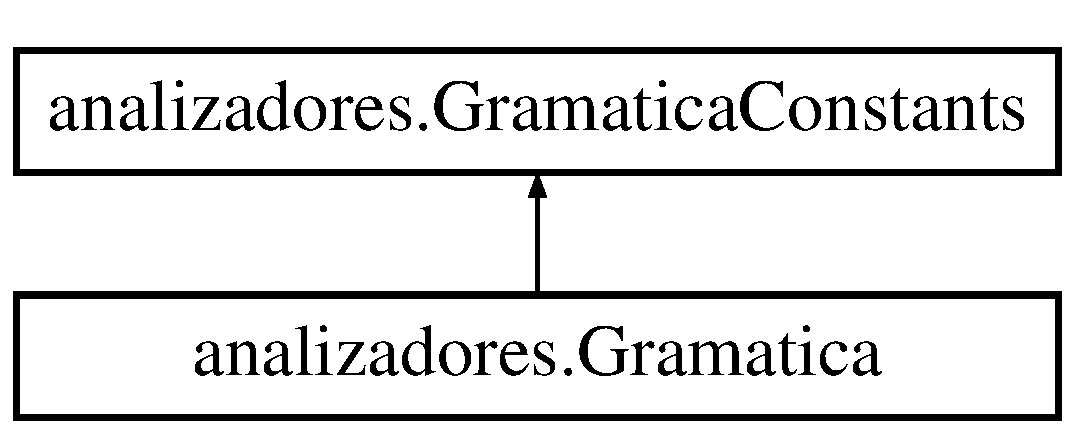
\includegraphics[height=2.000000cm]{classanalizadores_1_1_gramatica}
\end{center}
\end{figure}
\subsection*{Classes}
\begin{DoxyCompactItemize}
\item 
class {\bfseries J\+J\+Calls}
\end{DoxyCompactItemize}
\subsection*{Public Member Functions}
\begin{DoxyCompactItemize}
\item 
final Linked\+List$<$ \mbox{\hyperlink{interfaceast_1_1_nodo_a_s_t}{Nodo\+A\+ST}} $>$ \mbox{\hyperlink{classanalizadores_1_1_gramatica_a52ca5cd50acfbaffac4e463c71e8b7d0}{Analizar}} ()  throws Parse\+Exception 
\item 
final \mbox{\hyperlink{interfaceast_1_1_nodo_a_s_t}{Nodo\+A\+ST}} \mbox{\hyperlink{classanalizadores_1_1_gramatica_a9e84c347a44af8ef31e238a877e52eda}{Instruccion}} ()  throws Parse\+Exception 
\item 
\mbox{\Hypertarget{classanalizadores_1_1_gramatica_a10aec7ef38fd1abe23b6f07920e83541}\label{classanalizadores_1_1_gramatica_a10aec7ef38fd1abe23b6f07920e83541}} 
final \mbox{\hyperlink{interfaceast_1_1_instruccion}{Instruccion}} {\bfseries Funcion} ()  throws Parse\+Exception 
\item 
\mbox{\Hypertarget{classanalizadores_1_1_gramatica_aa0966b242f463d11350f4ca5962d84ed}\label{classanalizadores_1_1_gramatica_aa0966b242f463d11350f4ca5962d84ed}} 
final Linked\+List$<$ \mbox{\hyperlink{classentorno_1_1_simbolo}{Simbolo}} $>$ {\bfseries Lista\+\_\+\+Parametros} ()  throws Parse\+Exception 
\item 
\mbox{\Hypertarget{classanalizadores_1_1_gramatica_a2011491b79ad1d1ed63c2c6db45d7f14}\label{classanalizadores_1_1_gramatica_a2011491b79ad1d1ed63c2c6db45d7f14}} 
final \mbox{\hyperlink{classentorno_1_1_simbolo}{Simbolo}} {\bfseries Parametro} ()  throws Parse\+Exception 
\item 
final \mbox{\hyperlink{interfaceast_1_1_instruccion}{Instruccion}} \mbox{\hyperlink{classanalizadores_1_1_gramatica_a6ef9e58d753e27519e70a5f5085eb13b}{Asignacion}} ()  throws Parse\+Exception 
\item 
\mbox{\Hypertarget{classanalizadores_1_1_gramatica_a9e71d0f07af7ac12f5799832174a4dd4}\label{classanalizadores_1_1_gramatica_a9e71d0f07af7ac12f5799832174a4dd4}} 
final \mbox{\hyperlink{interfaceast_1_1_instruccion}{Instruccion}} {\bfseries Asignacion2} ()  throws Parse\+Exception 
\item 
\mbox{\Hypertarget{classanalizadores_1_1_gramatica_a8491b008d889445c8f9b170c3f4dd522}\label{classanalizadores_1_1_gramatica_a8491b008d889445c8f9b170c3f4dd522}} 
final \mbox{\hyperlink{interfaceast_1_1_expresion}{Expresion}} {\bfseries Retorno} ()  throws Parse\+Exception 
\item 
\mbox{\Hypertarget{classanalizadores_1_1_gramatica_a0ffdfae16a011d6191d93dabe0911df8}\label{classanalizadores_1_1_gramatica_a0ffdfae16a011d6191d93dabe0911df8}} 
final \mbox{\hyperlink{interfaceast_1_1_instruccion}{Instruccion}} {\bfseries detener} ()  throws Parse\+Exception 
\item 
\mbox{\Hypertarget{classanalizadores_1_1_gramatica_ae3c2611d1d90622f3696cedd88010c7e}\label{classanalizadores_1_1_gramatica_ae3c2611d1d90622f3696cedd88010c7e}} 
final \mbox{\hyperlink{interfaceast_1_1_instruccion}{Instruccion}} {\bfseries Continue} ()  throws Parse\+Exception 
\item 
\mbox{\Hypertarget{classanalizadores_1_1_gramatica_a4a77a7171a3fd0cd5eb8f9c4506afc39}\label{classanalizadores_1_1_gramatica_a4a77a7171a3fd0cd5eb8f9c4506afc39}} 
final \mbox{\hyperlink{interfaceast_1_1_instruccion}{Instruccion}} {\bfseries Mientras} ()  throws Parse\+Exception 
\item 
\mbox{\Hypertarget{classanalizadores_1_1_gramatica_a1ea41dc3dd72e5823b0e99a7fd0cc0ba}\label{classanalizadores_1_1_gramatica_a1ea41dc3dd72e5823b0e99a7fd0cc0ba}} 
final \mbox{\hyperlink{interfaceast_1_1_instruccion}{Instruccion}} {\bfseries Do\+Mientras} ()  throws Parse\+Exception 
\item 
\mbox{\Hypertarget{classanalizadores_1_1_gramatica_afe62720cfc2acacc9ddf158ad86d51cf}\label{classanalizadores_1_1_gramatica_afe62720cfc2acacc9ddf158ad86d51cf}} 
final \mbox{\hyperlink{interfaceast_1_1_instruccion}{Instruccion}} {\bfseries For} ()  throws Parse\+Exception 
\item 
\mbox{\Hypertarget{classanalizadores_1_1_gramatica_a28ef48d2daf3c88198bcc8872f5b5dfb}\label{classanalizadores_1_1_gramatica_a28ef48d2daf3c88198bcc8872f5b5dfb}} 
final \mbox{\hyperlink{interfaceast_1_1_instruccion}{Instruccion}} {\bfseries Si} ()  throws Parse\+Exception 
\item 
\mbox{\Hypertarget{classanalizadores_1_1_gramatica_acbab1ad9258b1765c0e75579cfa846a5}\label{classanalizadores_1_1_gramatica_acbab1ad9258b1765c0e75579cfa846a5}} 
final Linked\+List$<$ \mbox{\hyperlink{interfaceast_1_1_nodo_a_s_t}{Nodo\+A\+ST}} $>$ {\bfseries Bloque} ()  throws Parse\+Exception 
\item 
\mbox{\Hypertarget{classanalizadores_1_1_gramatica_a0aa1504c58e6b340527e36b69c271552}\label{classanalizadores_1_1_gramatica_a0aa1504c58e6b340527e36b69c271552}} 
final Linked\+List$<$ \mbox{\hyperlink{classentorno_1_1nodo_exp}{nodo\+Exp}} $>$ {\bfseries Dimensiones} ()  throws Parse\+Exception 
\item 
\mbox{\Hypertarget{classanalizadores_1_1_gramatica_ad2bacb82e3628dd63f0ba84c833d4a0f}\label{classanalizadores_1_1_gramatica_ad2bacb82e3628dd63f0ba84c833d4a0f}} 
final \mbox{\hyperlink{classentorno_1_1nodo_exp}{nodo\+Exp}} {\bfseries Dimension} ()  throws Parse\+Exception 
\item 
final \mbox{\hyperlink{interfaceast_1_1_nodo_a_s_t}{Nodo\+A\+ST}} \mbox{\hyperlink{classanalizadores_1_1_gramatica_adaa40a87451a4f0a9817d6aa699a29cc}{Llamada}} ()  throws Parse\+Exception 
\item 
final Linked\+List$<$ \mbox{\hyperlink{interfaceast_1_1_nodo_a_s_t}{Nodo\+A\+ST}} $>$ \mbox{\hyperlink{classanalizadores_1_1_gramatica_a85cf71aa91bab6d5875a0333d6c8eaa3}{Lista\+\_\+\+Expresiones}} ()  throws Parse\+Exception 
\item 
\mbox{\Hypertarget{classanalizadores_1_1_gramatica_a8665169171c61a43820eeb610185f2ef}\label{classanalizadores_1_1_gramatica_a8665169171c61a43820eeb610185f2ef}} 
final \mbox{\hyperlink{interfaceast_1_1_expresion}{Expresion}} {\bfseries E} ()  throws Parse\+Exception 
\item 
\mbox{\Hypertarget{classanalizadores_1_1_gramatica_ad179ebcc86755be93a364e113c57765a}\label{classanalizadores_1_1_gramatica_ad179ebcc86755be93a364e113c57765a}} 
final \mbox{\hyperlink{interfaceast_1_1_expresion}{Expresion}} {\bfseries Condicion\+Ternaria} ()  throws Parse\+Exception 
\item 
\mbox{\Hypertarget{classanalizadores_1_1_gramatica_abda840659e729a09678ee0da068f59b5}\label{classanalizadores_1_1_gramatica_abda840659e729a09678ee0da068f59b5}} 
final \mbox{\hyperlink{interfaceast_1_1_expresion}{Expresion}} {\bfseries Condicion\+And} ()  throws Parse\+Exception 
\item 
\mbox{\Hypertarget{classanalizadores_1_1_gramatica_a4d9394b7ae237631915860ee463cbaf3}\label{classanalizadores_1_1_gramatica_a4d9394b7ae237631915860ee463cbaf3}} 
final \mbox{\hyperlink{interfaceast_1_1_expresion}{Expresion}} {\bfseries Expresion\+Igualdad} ()  throws Parse\+Exception 
\item 
\mbox{\Hypertarget{classanalizadores_1_1_gramatica_a3ccc93c791ea000a8c1505a37940346b}\label{classanalizadores_1_1_gramatica_a3ccc93c791ea000a8c1505a37940346b}} 
final \mbox{\hyperlink{interfaceast_1_1_expresion}{Expresion}} {\bfseries Expresion\+Relacional} ()  throws Parse\+Exception 
\item 
\mbox{\Hypertarget{classanalizadores_1_1_gramatica_ad5fc8095ad59a56e0337b9ecacde8895}\label{classanalizadores_1_1_gramatica_ad5fc8095ad59a56e0337b9ecacde8895}} 
final \mbox{\hyperlink{interfaceast_1_1_expresion}{Expresion}} {\bfseries Expresion\+Aditiva} ()  throws Parse\+Exception 
\item 
\mbox{\Hypertarget{classanalizadores_1_1_gramatica_abea9e78545d093690b970a6a67c3ec50}\label{classanalizadores_1_1_gramatica_abea9e78545d093690b970a6a67c3ec50}} 
final \mbox{\hyperlink{interfaceast_1_1_expresion}{Expresion}} {\bfseries Expresion\+Multiplicativa} ()  throws Parse\+Exception 
\item 
\mbox{\Hypertarget{classanalizadores_1_1_gramatica_ae43002e54f4963541e7037f47eb90397}\label{classanalizadores_1_1_gramatica_ae43002e54f4963541e7037f47eb90397}} 
final \mbox{\hyperlink{interfaceast_1_1_expresion}{Expresion}} {\bfseries Expresion\+Potencia} ()  throws Parse\+Exception 
\item 
\mbox{\Hypertarget{classanalizadores_1_1_gramatica_a7eed7dc65e9f1fa51dfa49bfa7bc09b8}\label{classanalizadores_1_1_gramatica_a7eed7dc65e9f1fa51dfa49bfa7bc09b8}} 
final \mbox{\hyperlink{interfaceast_1_1_expresion}{Expresion}} {\bfseries Expresion\+Unaria} ()  throws Parse\+Exception 
\item 
final \mbox{\hyperlink{interfaceast_1_1_expresion}{Expresion}} \mbox{\hyperlink{classanalizadores_1_1_gramatica_ab82d652de277a9f80090631b30637b09}{Primitivo}} ()  throws Parse\+Exception 
\item 
\mbox{\hyperlink{classanalizadores_1_1_gramatica_a542f05b9164371cc73d1b9a7e70eb031}{Gramatica}} (java.\+io.\+Input\+Stream stream)
\item 
\mbox{\hyperlink{classanalizadores_1_1_gramatica_ad399a661121ef126e864fd65af3e290a}{Gramatica}} (java.\+io.\+Input\+Stream stream, String encoding)
\item 
void \mbox{\hyperlink{classanalizadores_1_1_gramatica_a2e933863c9692a4f638603bb43e87d14}{Re\+Init}} (java.\+io.\+Input\+Stream stream)
\item 
void \mbox{\hyperlink{classanalizadores_1_1_gramatica_a68a64ba7053949788dbe012722aea06b}{Re\+Init}} (java.\+io.\+Input\+Stream stream, String encoding)
\item 
\mbox{\hyperlink{classanalizadores_1_1_gramatica_aa27ae694010ecb86720e64791da67ad5}{Gramatica}} (java.\+io.\+Reader stream)
\item 
void \mbox{\hyperlink{classanalizadores_1_1_gramatica_ab2a19eaeba5ef605daa7c8ddaab5a01c}{Re\+Init}} (java.\+io.\+Reader stream)
\item 
\mbox{\hyperlink{classanalizadores_1_1_gramatica_a636956e2b18cbfd38cdb38432c625cbd}{Gramatica}} (\mbox{\hyperlink{classanalizadores_1_1_gramatica_token_manager}{Gramatica\+Token\+Manager}} tm)
\item 
void \mbox{\hyperlink{classanalizadores_1_1_gramatica_a92bab45b9e1fe815a3f87dc0d77ade38}{Re\+Init}} (\mbox{\hyperlink{classanalizadores_1_1_gramatica_token_manager}{Gramatica\+Token\+Manager}} tm)
\item 
final \mbox{\hyperlink{classanalizadores_1_1_token}{Token}} \mbox{\hyperlink{classanalizadores_1_1_gramatica_a9d110e08acaad0a9dafdb60f0bbab867}{get\+Next\+Token}} ()
\item 
final \mbox{\hyperlink{classanalizadores_1_1_token}{Token}} \mbox{\hyperlink{classanalizadores_1_1_gramatica_a58bb5ec9c1d432a2cc6194d6d829be8e}{get\+Token}} (int index)
\item 
\mbox{\hyperlink{classanalizadores_1_1_parse_exception}{Parse\+Exception}} \mbox{\hyperlink{classanalizadores_1_1_gramatica_a6052de1c7e91f9158b46025561ecd6cd}{generate\+Parse\+Exception}} ()
\item 
final void \mbox{\hyperlink{classanalizadores_1_1_gramatica_a6d0da3660603773438492f3be9406b48}{enable\+\_\+tracing}} ()
\item 
final void \mbox{\hyperlink{classanalizadores_1_1_gramatica_a5fafbda9430944314fe48e89f0d6a73a}{disable\+\_\+tracing}} ()
\end{DoxyCompactItemize}
\subsection*{Public Attributes}
\begin{DoxyCompactItemize}
\item 
\mbox{\hyperlink{classanalizadores_1_1_gramatica_token_manager}{Gramatica\+Token\+Manager}} \mbox{\hyperlink{classanalizadores_1_1_gramatica_a8f84a648c3c52e76b9dda324de4e8fb8}{token\+\_\+source}}
\item 
\mbox{\hyperlink{classanalizadores_1_1_token}{Token}} \mbox{\hyperlink{classanalizadores_1_1_gramatica_afceaf2a819c239c3f6ac455202a7bc58}{token}}
\item 
\mbox{\hyperlink{classanalizadores_1_1_token}{Token}} \mbox{\hyperlink{classanalizadores_1_1_gramatica_a0ed9c4bd78991e110d9cef4f8aeee5ee}{jj\+\_\+nt}}
\end{DoxyCompactItemize}


\subsection{Constructor \& Destructor Documentation}
\mbox{\Hypertarget{classanalizadores_1_1_gramatica_a542f05b9164371cc73d1b9a7e70eb031}\label{classanalizadores_1_1_gramatica_a542f05b9164371cc73d1b9a7e70eb031}} 
\index{analizadores\+::\+Gramatica@{analizadores\+::\+Gramatica}!Gramatica@{Gramatica}}
\index{Gramatica@{Gramatica}!analizadores\+::\+Gramatica@{analizadores\+::\+Gramatica}}
\subsubsection{\texorpdfstring{Gramatica()}{Gramatica()}\hspace{0.1cm}{\footnotesize\ttfamily [1/4]}}
{\footnotesize\ttfamily analizadores.\+Gramatica.\+Gramatica (\begin{DoxyParamCaption}\item[{java.\+io.\+Input\+Stream}]{stream }\end{DoxyParamCaption})}

Constructor with Input\+Stream. \mbox{\Hypertarget{classanalizadores_1_1_gramatica_ad399a661121ef126e864fd65af3e290a}\label{classanalizadores_1_1_gramatica_ad399a661121ef126e864fd65af3e290a}} 
\index{analizadores\+::\+Gramatica@{analizadores\+::\+Gramatica}!Gramatica@{Gramatica}}
\index{Gramatica@{Gramatica}!analizadores\+::\+Gramatica@{analizadores\+::\+Gramatica}}
\subsubsection{\texorpdfstring{Gramatica()}{Gramatica()}\hspace{0.1cm}{\footnotesize\ttfamily [2/4]}}
{\footnotesize\ttfamily analizadores.\+Gramatica.\+Gramatica (\begin{DoxyParamCaption}\item[{java.\+io.\+Input\+Stream}]{stream,  }\item[{String}]{encoding }\end{DoxyParamCaption})}

Constructor with Input\+Stream and supplied encoding \mbox{\Hypertarget{classanalizadores_1_1_gramatica_aa27ae694010ecb86720e64791da67ad5}\label{classanalizadores_1_1_gramatica_aa27ae694010ecb86720e64791da67ad5}} 
\index{analizadores\+::\+Gramatica@{analizadores\+::\+Gramatica}!Gramatica@{Gramatica}}
\index{Gramatica@{Gramatica}!analizadores\+::\+Gramatica@{analizadores\+::\+Gramatica}}
\subsubsection{\texorpdfstring{Gramatica()}{Gramatica()}\hspace{0.1cm}{\footnotesize\ttfamily [3/4]}}
{\footnotesize\ttfamily analizadores.\+Gramatica.\+Gramatica (\begin{DoxyParamCaption}\item[{java.\+io.\+Reader}]{stream }\end{DoxyParamCaption})}

Constructor. \mbox{\Hypertarget{classanalizadores_1_1_gramatica_a636956e2b18cbfd38cdb38432c625cbd}\label{classanalizadores_1_1_gramatica_a636956e2b18cbfd38cdb38432c625cbd}} 
\index{analizadores\+::\+Gramatica@{analizadores\+::\+Gramatica}!Gramatica@{Gramatica}}
\index{Gramatica@{Gramatica}!analizadores\+::\+Gramatica@{analizadores\+::\+Gramatica}}
\subsubsection{\texorpdfstring{Gramatica()}{Gramatica()}\hspace{0.1cm}{\footnotesize\ttfamily [4/4]}}
{\footnotesize\ttfamily analizadores.\+Gramatica.\+Gramatica (\begin{DoxyParamCaption}\item[{\mbox{\hyperlink{classanalizadores_1_1_gramatica_token_manager}{Gramatica\+Token\+Manager}}}]{tm }\end{DoxyParamCaption})}

Constructor with generated \mbox{\hyperlink{classanalizadores_1_1_token}{Token}} Manager. 

\subsection{Member Function Documentation}
\mbox{\Hypertarget{classanalizadores_1_1_gramatica_a52ca5cd50acfbaffac4e463c71e8b7d0}\label{classanalizadores_1_1_gramatica_a52ca5cd50acfbaffac4e463c71e8b7d0}} 
\index{analizadores\+::\+Gramatica@{analizadores\+::\+Gramatica}!Analizar@{Analizar}}
\index{Analizar@{Analizar}!analizadores\+::\+Gramatica@{analizadores\+::\+Gramatica}}
\subsubsection{\texorpdfstring{Analizar()}{Analizar()}}
{\footnotesize\ttfamily final Linked\+List$<$\mbox{\hyperlink{interfaceast_1_1_nodo_a_s_t}{Nodo\+A\+ST}}$>$ analizadores.\+Gramatica.\+Analizar (\begin{DoxyParamCaption}{ }\end{DoxyParamCaption}) throws \mbox{\hyperlink{classanalizadores_1_1_parse_exception}{Parse\+Exception}}}

Fin \mbox{\hyperlink{classanalizadores_1_1_lexico}{Lexico}} Producción inicial Analizar -\/$>$ (Instruccion)+ E\+OF \mbox{\Hypertarget{classanalizadores_1_1_gramatica_a6ef9e58d753e27519e70a5f5085eb13b}\label{classanalizadores_1_1_gramatica_a6ef9e58d753e27519e70a5f5085eb13b}} 
\index{analizadores\+::\+Gramatica@{analizadores\+::\+Gramatica}!Asignacion@{Asignacion}}
\index{Asignacion@{Asignacion}!analizadores\+::\+Gramatica@{analizadores\+::\+Gramatica}}
\subsubsection{\texorpdfstring{Asignacion()}{Asignacion()}}
{\footnotesize\ttfamily final \mbox{\hyperlink{interfaceast_1_1_instruccion}{Instruccion}} analizadores.\+Gramatica.\+Asignacion (\begin{DoxyParamCaption}{ }\end{DoxyParamCaption}) throws \mbox{\hyperlink{classanalizadores_1_1_parse_exception}{Parse\+Exception}}}

Asignacion -\/$>$ id = expresion; $\vert$id D\+IM = E\+XP \mbox{\Hypertarget{classanalizadores_1_1_gramatica_a5fafbda9430944314fe48e89f0d6a73a}\label{classanalizadores_1_1_gramatica_a5fafbda9430944314fe48e89f0d6a73a}} 
\index{analizadores\+::\+Gramatica@{analizadores\+::\+Gramatica}!disable\+\_\+tracing@{disable\+\_\+tracing}}
\index{disable\+\_\+tracing@{disable\+\_\+tracing}!analizadores\+::\+Gramatica@{analizadores\+::\+Gramatica}}
\subsubsection{\texorpdfstring{disable\+\_\+tracing()}{disable\_tracing()}}
{\footnotesize\ttfamily final void analizadores.\+Gramatica.\+disable\+\_\+tracing (\begin{DoxyParamCaption}{ }\end{DoxyParamCaption})}

Disable tracing. \mbox{\Hypertarget{classanalizadores_1_1_gramatica_a6d0da3660603773438492f3be9406b48}\label{classanalizadores_1_1_gramatica_a6d0da3660603773438492f3be9406b48}} 
\index{analizadores\+::\+Gramatica@{analizadores\+::\+Gramatica}!enable\+\_\+tracing@{enable\+\_\+tracing}}
\index{enable\+\_\+tracing@{enable\+\_\+tracing}!analizadores\+::\+Gramatica@{analizadores\+::\+Gramatica}}
\subsubsection{\texorpdfstring{enable\+\_\+tracing()}{enable\_tracing()}}
{\footnotesize\ttfamily final void analizadores.\+Gramatica.\+enable\+\_\+tracing (\begin{DoxyParamCaption}{ }\end{DoxyParamCaption})}

Enable tracing. \mbox{\Hypertarget{classanalizadores_1_1_gramatica_a6052de1c7e91f9158b46025561ecd6cd}\label{classanalizadores_1_1_gramatica_a6052de1c7e91f9158b46025561ecd6cd}} 
\index{analizadores\+::\+Gramatica@{analizadores\+::\+Gramatica}!generate\+Parse\+Exception@{generate\+Parse\+Exception}}
\index{generate\+Parse\+Exception@{generate\+Parse\+Exception}!analizadores\+::\+Gramatica@{analizadores\+::\+Gramatica}}
\subsubsection{\texorpdfstring{generate\+Parse\+Exception()}{generateParseException()}}
{\footnotesize\ttfamily \mbox{\hyperlink{classanalizadores_1_1_parse_exception}{Parse\+Exception}} analizadores.\+Gramatica.\+generate\+Parse\+Exception (\begin{DoxyParamCaption}{ }\end{DoxyParamCaption})}

Generate \mbox{\hyperlink{classanalizadores_1_1_parse_exception}{Parse\+Exception}}. \mbox{\Hypertarget{classanalizadores_1_1_gramatica_a9d110e08acaad0a9dafdb60f0bbab867}\label{classanalizadores_1_1_gramatica_a9d110e08acaad0a9dafdb60f0bbab867}} 
\index{analizadores\+::\+Gramatica@{analizadores\+::\+Gramatica}!get\+Next\+Token@{get\+Next\+Token}}
\index{get\+Next\+Token@{get\+Next\+Token}!analizadores\+::\+Gramatica@{analizadores\+::\+Gramatica}}
\subsubsection{\texorpdfstring{get\+Next\+Token()}{getNextToken()}}
{\footnotesize\ttfamily final \mbox{\hyperlink{classanalizadores_1_1_token}{Token}} analizadores.\+Gramatica.\+get\+Next\+Token (\begin{DoxyParamCaption}{ }\end{DoxyParamCaption})}

Get the next \mbox{\hyperlink{classanalizadores_1_1_token}{Token}}. \mbox{\Hypertarget{classanalizadores_1_1_gramatica_a58bb5ec9c1d432a2cc6194d6d829be8e}\label{classanalizadores_1_1_gramatica_a58bb5ec9c1d432a2cc6194d6d829be8e}} 
\index{analizadores\+::\+Gramatica@{analizadores\+::\+Gramatica}!get\+Token@{get\+Token}}
\index{get\+Token@{get\+Token}!analizadores\+::\+Gramatica@{analizadores\+::\+Gramatica}}
\subsubsection{\texorpdfstring{get\+Token()}{getToken()}}
{\footnotesize\ttfamily final \mbox{\hyperlink{classanalizadores_1_1_token}{Token}} analizadores.\+Gramatica.\+get\+Token (\begin{DoxyParamCaption}\item[{int}]{index }\end{DoxyParamCaption})}

Get the specific \mbox{\hyperlink{classanalizadores_1_1_token}{Token}}. \mbox{\Hypertarget{classanalizadores_1_1_gramatica_a9e84c347a44af8ef31e238a877e52eda}\label{classanalizadores_1_1_gramatica_a9e84c347a44af8ef31e238a877e52eda}} 
\index{analizadores\+::\+Gramatica@{analizadores\+::\+Gramatica}!Instruccion@{Instruccion}}
\index{Instruccion@{Instruccion}!analizadores\+::\+Gramatica@{analizadores\+::\+Gramatica}}
\subsubsection{\texorpdfstring{Instruccion()}{Instruccion()}}
{\footnotesize\ttfamily final \mbox{\hyperlink{interfaceast_1_1_nodo_a_s_t}{Nodo\+A\+ST}} analizadores.\+Gramatica.\+Instruccion (\begin{DoxyParamCaption}{ }\end{DoxyParamCaption}) throws \mbox{\hyperlink{classanalizadores_1_1_parse_exception}{Parse\+Exception}}}

Instruccion -\/$>$ Llamada $\vert$ asignacion \mbox{\Hypertarget{classanalizadores_1_1_gramatica_a85cf71aa91bab6d5875a0333d6c8eaa3}\label{classanalizadores_1_1_gramatica_a85cf71aa91bab6d5875a0333d6c8eaa3}} 
\index{analizadores\+::\+Gramatica@{analizadores\+::\+Gramatica}!Lista\+\_\+\+Expresiones@{Lista\+\_\+\+Expresiones}}
\index{Lista\+\_\+\+Expresiones@{Lista\+\_\+\+Expresiones}!analizadores\+::\+Gramatica@{analizadores\+::\+Gramatica}}
\subsubsection{\texorpdfstring{Lista\+\_\+\+Expresiones()}{Lista\_Expresiones()}}
{\footnotesize\ttfamily final Linked\+List$<$\mbox{\hyperlink{interfaceast_1_1_nodo_a_s_t}{Nodo\+A\+ST}}$>$ analizadores.\+Gramatica.\+Lista\+\_\+\+Expresiones (\begin{DoxyParamCaption}{ }\end{DoxyParamCaption}) throws \mbox{\hyperlink{classanalizadores_1_1_parse_exception}{Parse\+Exception}}}

Lista\+\_\+\+Expresiones -\/$>$ Expresion ( , )$\ast$; \mbox{\Hypertarget{classanalizadores_1_1_gramatica_adaa40a87451a4f0a9817d6aa699a29cc}\label{classanalizadores_1_1_gramatica_adaa40a87451a4f0a9817d6aa699a29cc}} 
\index{analizadores\+::\+Gramatica@{analizadores\+::\+Gramatica}!Llamada@{Llamada}}
\index{Llamada@{Llamada}!analizadores\+::\+Gramatica@{analizadores\+::\+Gramatica}}
\subsubsection{\texorpdfstring{Llamada()}{Llamada()}}
{\footnotesize\ttfamily final \mbox{\hyperlink{interfaceast_1_1_nodo_a_s_t}{Nodo\+A\+ST}} analizadores.\+Gramatica.\+Llamada (\begin{DoxyParamCaption}{ }\end{DoxyParamCaption}) throws \mbox{\hyperlink{classanalizadores_1_1_parse_exception}{Parse\+Exception}}}

Llamada -\/$>$ print ( Expresion ); \mbox{\Hypertarget{classanalizadores_1_1_gramatica_ab82d652de277a9f80090631b30637b09}\label{classanalizadores_1_1_gramatica_ab82d652de277a9f80090631b30637b09}} 
\index{analizadores\+::\+Gramatica@{analizadores\+::\+Gramatica}!Primitivo@{Primitivo}}
\index{Primitivo@{Primitivo}!analizadores\+::\+Gramatica@{analizadores\+::\+Gramatica}}
\subsubsection{\texorpdfstring{Primitivo()}{Primitivo()}}
{\footnotesize\ttfamily final \mbox{\hyperlink{interfaceast_1_1_expresion}{Expresion}} analizadores.\+Gramatica.\+Primitivo (\begin{DoxyParamCaption}{ }\end{DoxyParamCaption}) throws \mbox{\hyperlink{classanalizadores_1_1_parse_exception}{Parse\+Exception}}}

Primitivo -\/$>$ Numero $\vert$ Decimal $\vert$ \textquotesingle{}(\textquotesingle{} Expresion \textquotesingle{})\textquotesingle{} \mbox{\Hypertarget{classanalizadores_1_1_gramatica_a2e933863c9692a4f638603bb43e87d14}\label{classanalizadores_1_1_gramatica_a2e933863c9692a4f638603bb43e87d14}} 
\index{analizadores\+::\+Gramatica@{analizadores\+::\+Gramatica}!Re\+Init@{Re\+Init}}
\index{Re\+Init@{Re\+Init}!analizadores\+::\+Gramatica@{analizadores\+::\+Gramatica}}
\subsubsection{\texorpdfstring{Re\+Init()}{ReInit()}\hspace{0.1cm}{\footnotesize\ttfamily [1/4]}}
{\footnotesize\ttfamily void analizadores.\+Gramatica.\+Re\+Init (\begin{DoxyParamCaption}\item[{java.\+io.\+Input\+Stream}]{stream }\end{DoxyParamCaption})}

Reinitialise. \mbox{\Hypertarget{classanalizadores_1_1_gramatica_a68a64ba7053949788dbe012722aea06b}\label{classanalizadores_1_1_gramatica_a68a64ba7053949788dbe012722aea06b}} 
\index{analizadores\+::\+Gramatica@{analizadores\+::\+Gramatica}!Re\+Init@{Re\+Init}}
\index{Re\+Init@{Re\+Init}!analizadores\+::\+Gramatica@{analizadores\+::\+Gramatica}}
\subsubsection{\texorpdfstring{Re\+Init()}{ReInit()}\hspace{0.1cm}{\footnotesize\ttfamily [2/4]}}
{\footnotesize\ttfamily void analizadores.\+Gramatica.\+Re\+Init (\begin{DoxyParamCaption}\item[{java.\+io.\+Input\+Stream}]{stream,  }\item[{String}]{encoding }\end{DoxyParamCaption})}

Reinitialise. \mbox{\Hypertarget{classanalizadores_1_1_gramatica_ab2a19eaeba5ef605daa7c8ddaab5a01c}\label{classanalizadores_1_1_gramatica_ab2a19eaeba5ef605daa7c8ddaab5a01c}} 
\index{analizadores\+::\+Gramatica@{analizadores\+::\+Gramatica}!Re\+Init@{Re\+Init}}
\index{Re\+Init@{Re\+Init}!analizadores\+::\+Gramatica@{analizadores\+::\+Gramatica}}
\subsubsection{\texorpdfstring{Re\+Init()}{ReInit()}\hspace{0.1cm}{\footnotesize\ttfamily [3/4]}}
{\footnotesize\ttfamily void analizadores.\+Gramatica.\+Re\+Init (\begin{DoxyParamCaption}\item[{java.\+io.\+Reader}]{stream }\end{DoxyParamCaption})}

Reinitialise. \mbox{\Hypertarget{classanalizadores_1_1_gramatica_a92bab45b9e1fe815a3f87dc0d77ade38}\label{classanalizadores_1_1_gramatica_a92bab45b9e1fe815a3f87dc0d77ade38}} 
\index{analizadores\+::\+Gramatica@{analizadores\+::\+Gramatica}!Re\+Init@{Re\+Init}}
\index{Re\+Init@{Re\+Init}!analizadores\+::\+Gramatica@{analizadores\+::\+Gramatica}}
\subsubsection{\texorpdfstring{Re\+Init()}{ReInit()}\hspace{0.1cm}{\footnotesize\ttfamily [4/4]}}
{\footnotesize\ttfamily void analizadores.\+Gramatica.\+Re\+Init (\begin{DoxyParamCaption}\item[{\mbox{\hyperlink{classanalizadores_1_1_gramatica_token_manager}{Gramatica\+Token\+Manager}}}]{tm }\end{DoxyParamCaption})}

Reinitialise. 

\subsection{Member Data Documentation}
\mbox{\Hypertarget{classanalizadores_1_1_gramatica_a0ed9c4bd78991e110d9cef4f8aeee5ee}\label{classanalizadores_1_1_gramatica_a0ed9c4bd78991e110d9cef4f8aeee5ee}} 
\index{analizadores\+::\+Gramatica@{analizadores\+::\+Gramatica}!jj\+\_\+nt@{jj\+\_\+nt}}
\index{jj\+\_\+nt@{jj\+\_\+nt}!analizadores\+::\+Gramatica@{analizadores\+::\+Gramatica}}
\subsubsection{\texorpdfstring{jj\+\_\+nt}{jj\_nt}}
{\footnotesize\ttfamily \mbox{\hyperlink{classanalizadores_1_1_token}{Token}} analizadores.\+Gramatica.\+jj\+\_\+nt}

Next token. \mbox{\Hypertarget{classanalizadores_1_1_gramatica_afceaf2a819c239c3f6ac455202a7bc58}\label{classanalizadores_1_1_gramatica_afceaf2a819c239c3f6ac455202a7bc58}} 
\index{analizadores\+::\+Gramatica@{analizadores\+::\+Gramatica}!token@{token}}
\index{token@{token}!analizadores\+::\+Gramatica@{analizadores\+::\+Gramatica}}
\subsubsection{\texorpdfstring{token}{token}}
{\footnotesize\ttfamily \mbox{\hyperlink{classanalizadores_1_1_token}{Token}} analizadores.\+Gramatica.\+token}

Current token. \mbox{\Hypertarget{classanalizadores_1_1_gramatica_a8f84a648c3c52e76b9dda324de4e8fb8}\label{classanalizadores_1_1_gramatica_a8f84a648c3c52e76b9dda324de4e8fb8}} 
\index{analizadores\+::\+Gramatica@{analizadores\+::\+Gramatica}!token\+\_\+source@{token\+\_\+source}}
\index{token\+\_\+source@{token\+\_\+source}!analizadores\+::\+Gramatica@{analizadores\+::\+Gramatica}}
\subsubsection{\texorpdfstring{token\+\_\+source}{token\_source}}
{\footnotesize\ttfamily \mbox{\hyperlink{classanalizadores_1_1_gramatica_token_manager}{Gramatica\+Token\+Manager}} analizadores.\+Gramatica.\+token\+\_\+source}

Generated \mbox{\hyperlink{classanalizadores_1_1_token}{Token}} Manager. 

The documentation for this class was generated from the following file\+:\begin{DoxyCompactItemize}
\item 
src/analizadores/Gramatica.\+java\end{DoxyCompactItemize}

\hypertarget{interfaceanalizadores_1_1_gramatica_constants}{}\section{analizadores.\+Gramatica\+Constants Interface Reference}
\label{interfaceanalizadores_1_1_gramatica_constants}\index{analizadores.\+Gramatica\+Constants@{analizadores.\+Gramatica\+Constants}}
Inheritance diagram for analizadores.\+Gramatica\+Constants\+:\begin{figure}[H]
\begin{center}
\leavevmode
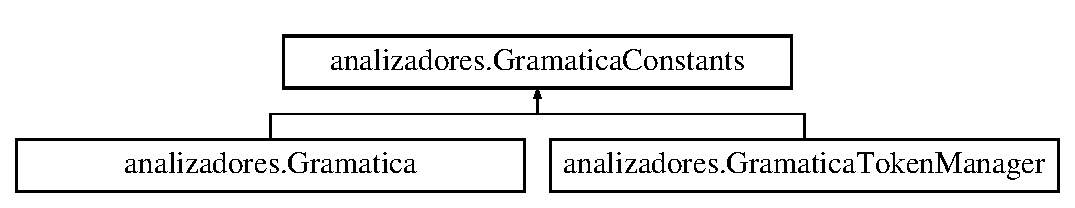
\includegraphics[height=2.000000cm]{interfaceanalizadores_1_1_gramatica_constants}
\end{center}
\end{figure}
\subsection*{Public Attributes}
\begin{DoxyCompactItemize}
\item 
int \mbox{\hyperlink{interfaceanalizadores_1_1_gramatica_constants_a78849fabb7f96d877057df7bc842f18e}{E\+OF}} = 0
\item 
int \mbox{\hyperlink{interfaceanalizadores_1_1_gramatica_constants_a2bb08e3061d1cbbbc62bd109fea7d306}{M\+I\+E\+N\+T\+R\+AS}} = 1
\item 
int \mbox{\hyperlink{interfaceanalizadores_1_1_gramatica_constants_a07821a423cc437fe2fd22edd7f4ec5d8}{DO}} = 2
\item 
int \mbox{\hyperlink{interfaceanalizadores_1_1_gramatica_constants_a981f1c14f28166e55b0a31b26b0b0e83}{F\+U\+N\+C\+I\+ON}} = 3
\item 
int \mbox{\hyperlink{interfaceanalizadores_1_1_gramatica_constants_a04405a6ab5d03ee083a65c067cb476a6}{R\+E\+T\+O\+R\+NO}} = 4
\item 
int \mbox{\hyperlink{interfaceanalizadores_1_1_gramatica_constants_aaf66e077637af9181c9d21b11b842ad3}{F\+OR}} = 5
\item 
int \mbox{\hyperlink{interfaceanalizadores_1_1_gramatica_constants_a0074ea97516624677218650e453db212}{B\+R\+E\+AK}} = 6
\item 
int \mbox{\hyperlink{interfaceanalizadores_1_1_gramatica_constants_a33b0c0fcbd620e83d8e8b57163bfcd8c}{C\+O\+N\+T\+I\+N\+UE}} = 7
\item 
int \mbox{\hyperlink{interfaceanalizadores_1_1_gramatica_constants_a989aff00f85aedf3c451be5dfd7d9181}{SI}} = 8
\item 
int \mbox{\hyperlink{interfaceanalizadores_1_1_gramatica_constants_ab6beefe470534d1183471e82195f52d5}{S\+I\+NO}} = 9
\item 
int \mbox{\hyperlink{interfaceanalizadores_1_1_gramatica_constants_a24400027cdf8750bdb27f414806f66f0}{T\+R\+UE}} = 10
\item 
int \mbox{\hyperlink{interfaceanalizadores_1_1_gramatica_constants_ab68bef741cc34a342d22b7918964be5c}{F\+A\+L\+SE}} = 11
\item 
int \mbox{\hyperlink{interfaceanalizadores_1_1_gramatica_constants_a30b827671b3dc645fe5cc79a4b2ed46a}{N\+U\+LL}} = 12
\item 
int \mbox{\hyperlink{interfaceanalizadores_1_1_gramatica_constants_acff59f75d71d957b9930f91d75fd5038}{IN}} = 13
\item 
int \mbox{\hyperlink{interfaceanalizadores_1_1_gramatica_constants_aa69e02b866b107cfd186f5fcbba9ac51}{D\+E\+FA}} = 14
\item 
int \mbox{\hyperlink{interfaceanalizadores_1_1_gramatica_constants_abc9e0a63b989075c0213e44b8e223ea4}{P\+C\+O\+MA}} = 15
\item 
int \mbox{\hyperlink{interfaceanalizadores_1_1_gramatica_constants_acedde7841bc5ca1f5146d750b47496c5}{C\+O\+MA}} = 16
\item 
int \mbox{\hyperlink{interfaceanalizadores_1_1_gramatica_constants_afdcc2c9f3f0130b7b0486817c6937d9f}{P\+A\+R\+E\+NI}} = 17
\item 
int \mbox{\hyperlink{interfaceanalizadores_1_1_gramatica_constants_ac51cc285e134d68eaee01bd65ecdd7bb}{P\+A\+R\+E\+ND}} = 18
\item 
int \mbox{\hyperlink{interfaceanalizadores_1_1_gramatica_constants_a76ab9fe9bd12cafb7deb930e14988995}{C\+O\+RI}} = 19
\item 
int \mbox{\hyperlink{interfaceanalizadores_1_1_gramatica_constants_a51702aa079a81a977d0028a2909880eb}{C\+O\+RD}} = 20
\item 
int \mbox{\hyperlink{interfaceanalizadores_1_1_gramatica_constants_ae8ba08b4bf4c02c11eea86d29b9e5445}{L\+L\+A\+V\+EI}} = 21
\item 
int \mbox{\hyperlink{interfaceanalizadores_1_1_gramatica_constants_acffaab6940663977d8fb24696d63785b}{L\+L\+A\+V\+ED}} = 22
\item 
int \mbox{\hyperlink{interfaceanalizadores_1_1_gramatica_constants_a3e5bf3d5cda5189d03224395690e752c}{T\+E\+R\+N\+A\+R\+IO}} = 23
\item 
int \mbox{\hyperlink{interfaceanalizadores_1_1_gramatica_constants_a2eb26f040e7e8b0298b5787db7383d69}{D\+O\+S\+P\+U\+N\+T\+OS}} = 24
\item 
int \mbox{\hyperlink{interfaceanalizadores_1_1_gramatica_constants_ab01f84d702322d13371eeb7af0c00208}{M\+AS}} = 25
\item 
int \mbox{\hyperlink{interfaceanalizadores_1_1_gramatica_constants_ad081af20fa889403e88f484a9637591b}{M\+E\+N\+OS}} = 26
\item 
int \mbox{\hyperlink{interfaceanalizadores_1_1_gramatica_constants_a543556c9302bd7745f419c23682a18b9}{P\+OR}} = 27
\item 
int \mbox{\hyperlink{interfaceanalizadores_1_1_gramatica_constants_ae48180a1943669c4236d40af2eb9110a}{M\+O\+D\+U\+LO}} = 28
\item 
int \mbox{\hyperlink{interfaceanalizadores_1_1_gramatica_constants_a6610a09833080b2a5970723499323e6e}{D\+IV}} = 29
\item 
int \mbox{\hyperlink{interfaceanalizadores_1_1_gramatica_constants_a1ae500dd74e522b0250a020110052b12}{P\+O\+T\+E\+N\+C\+IA}} = 30
\item 
int \mbox{\hyperlink{interfaceanalizadores_1_1_gramatica_constants_aac72eeab2f4935ecb78c6b3b17019122}{I\+G\+U\+AL}} = 31
\item 
int \mbox{\hyperlink{interfaceanalizadores_1_1_gramatica_constants_a65f84acb0f1ab5f34356859a4f07558f}{M\+E\+N\+O\+R\+Q\+UE}} = 32
\item 
int \mbox{\hyperlink{interfaceanalizadores_1_1_gramatica_constants_aacb74771dc1cb12eba87a6514ca08194}{M\+A\+Y\+O\+R\+Q\+UE}} = 33
\item 
int \mbox{\hyperlink{interfaceanalizadores_1_1_gramatica_constants_a839bf03446ac33a6b6a7efb5a7f7f6bf}{M\+E\+N\+O\+R\+I\+G\+U\+AL}} = 34
\item 
int \mbox{\hyperlink{interfaceanalizadores_1_1_gramatica_constants_aea3102747f33a3cea9c8ad1bc5ed367c}{M\+A\+Y\+O\+R\+I\+G\+U\+AL}} = 35
\item 
int \mbox{\hyperlink{interfaceanalizadores_1_1_gramatica_constants_aa67702fd19eaeb7b4fe930931e253de9}{I\+G\+U\+A\+L\+A\+C\+I\+ON}} = 36
\item 
int \mbox{\hyperlink{interfaceanalizadores_1_1_gramatica_constants_a28adc7022b6c3a6389fa98ffe04070c7}{D\+I\+F\+E\+R\+E\+N\+C\+I\+A\+C\+I\+ON}} = 37
\item 
int \mbox{\hyperlink{interfaceanalizadores_1_1_gramatica_constants_a7fd3bdfec25ae81f32b643b9fe052ef8}{A\+ND}} = 38
\item 
int \mbox{\hyperlink{interfaceanalizadores_1_1_gramatica_constants_ae08f59cb767c3d76286207642b31b139}{OR}} = 39
\item 
int \mbox{\hyperlink{interfaceanalizadores_1_1_gramatica_constants_ad271ffcb451fea619aace92e6a724b10}{N\+OT}} = 40
\item 
int \mbox{\hyperlink{interfaceanalizadores_1_1_gramatica_constants_a2cba48faced5c33b817a83d7bfb0e01c}{N\+U\+M\+E\+RO}} = 41
\item 
int \mbox{\hyperlink{interfaceanalizadores_1_1_gramatica_constants_a749a4c57e0c04da4446d95e655d2dc91}{D\+E\+C\+I\+M\+AL}} = 42
\item 
int \mbox{\hyperlink{interfaceanalizadores_1_1_gramatica_constants_aab0202a37664dca424e05af64e64921d}{ID}} = 43
\item 
int \mbox{\hyperlink{interfaceanalizadores_1_1_gramatica_constants_ac01d6927feb2b99c514f5c1fe4d49b66}{S\+T\+R\+I\+NG}} = 53
\item 
int \mbox{\hyperlink{interfaceanalizadores_1_1_gramatica_constants_abca71964b246eaad16d419905d464b46}{D\+E\+F\+A\+U\+LT}} = 0
\item 
int \mbox{\hyperlink{interfaceanalizadores_1_1_gramatica_constants_a27b5c5393e6763f57f2fe03547a05fa7}{S\+T\+R\+I\+N\+G\+\_\+\+S\+T\+A\+TE}} = 1
\item 
String \mbox{[}$\,$\mbox{]} \mbox{\hyperlink{interfaceanalizadores_1_1_gramatica_constants_a9836f388bc00746d299a14a9529474bc}{token\+Image}}
\end{DoxyCompactItemize}


\subsection{Detailed Description}
\mbox{\hyperlink{classanalizadores_1_1_token}{Token}} literal values and constants. Generated by org.\+javacc.\+parser.\+Other\+Files\+Gen\+::start() 

\subsection{Member Data Documentation}
\mbox{\Hypertarget{interfaceanalizadores_1_1_gramatica_constants_a7fd3bdfec25ae81f32b643b9fe052ef8}\label{interfaceanalizadores_1_1_gramatica_constants_a7fd3bdfec25ae81f32b643b9fe052ef8}} 
\index{analizadores\+::\+Gramatica\+Constants@{analizadores\+::\+Gramatica\+Constants}!A\+ND@{A\+ND}}
\index{A\+ND@{A\+ND}!analizadores\+::\+Gramatica\+Constants@{analizadores\+::\+Gramatica\+Constants}}
\subsubsection{\texorpdfstring{A\+ND}{AND}}
{\footnotesize\ttfamily int analizadores.\+Gramatica\+Constants.\+A\+ND = 38}

Regular\+Expression Id. \mbox{\Hypertarget{interfaceanalizadores_1_1_gramatica_constants_a0074ea97516624677218650e453db212}\label{interfaceanalizadores_1_1_gramatica_constants_a0074ea97516624677218650e453db212}} 
\index{analizadores\+::\+Gramatica\+Constants@{analizadores\+::\+Gramatica\+Constants}!B\+R\+E\+AK@{B\+R\+E\+AK}}
\index{B\+R\+E\+AK@{B\+R\+E\+AK}!analizadores\+::\+Gramatica\+Constants@{analizadores\+::\+Gramatica\+Constants}}
\subsubsection{\texorpdfstring{B\+R\+E\+AK}{BREAK}}
{\footnotesize\ttfamily int analizadores.\+Gramatica\+Constants.\+B\+R\+E\+AK = 6}

Regular\+Expression Id. \mbox{\Hypertarget{interfaceanalizadores_1_1_gramatica_constants_acedde7841bc5ca1f5146d750b47496c5}\label{interfaceanalizadores_1_1_gramatica_constants_acedde7841bc5ca1f5146d750b47496c5}} 
\index{analizadores\+::\+Gramatica\+Constants@{analizadores\+::\+Gramatica\+Constants}!C\+O\+MA@{C\+O\+MA}}
\index{C\+O\+MA@{C\+O\+MA}!analizadores\+::\+Gramatica\+Constants@{analizadores\+::\+Gramatica\+Constants}}
\subsubsection{\texorpdfstring{C\+O\+MA}{COMA}}
{\footnotesize\ttfamily int analizadores.\+Gramatica\+Constants.\+C\+O\+MA = 16}

Regular\+Expression Id. \mbox{\Hypertarget{interfaceanalizadores_1_1_gramatica_constants_a33b0c0fcbd620e83d8e8b57163bfcd8c}\label{interfaceanalizadores_1_1_gramatica_constants_a33b0c0fcbd620e83d8e8b57163bfcd8c}} 
\index{analizadores\+::\+Gramatica\+Constants@{analizadores\+::\+Gramatica\+Constants}!C\+O\+N\+T\+I\+N\+UE@{C\+O\+N\+T\+I\+N\+UE}}
\index{C\+O\+N\+T\+I\+N\+UE@{C\+O\+N\+T\+I\+N\+UE}!analizadores\+::\+Gramatica\+Constants@{analizadores\+::\+Gramatica\+Constants}}
\subsubsection{\texorpdfstring{C\+O\+N\+T\+I\+N\+UE}{CONTINUE}}
{\footnotesize\ttfamily int analizadores.\+Gramatica\+Constants.\+C\+O\+N\+T\+I\+N\+UE = 7}

Regular\+Expression Id. \mbox{\Hypertarget{interfaceanalizadores_1_1_gramatica_constants_a51702aa079a81a977d0028a2909880eb}\label{interfaceanalizadores_1_1_gramatica_constants_a51702aa079a81a977d0028a2909880eb}} 
\index{analizadores\+::\+Gramatica\+Constants@{analizadores\+::\+Gramatica\+Constants}!C\+O\+RD@{C\+O\+RD}}
\index{C\+O\+RD@{C\+O\+RD}!analizadores\+::\+Gramatica\+Constants@{analizadores\+::\+Gramatica\+Constants}}
\subsubsection{\texorpdfstring{C\+O\+RD}{CORD}}
{\footnotesize\ttfamily int analizadores.\+Gramatica\+Constants.\+C\+O\+RD = 20}

Regular\+Expression Id. \mbox{\Hypertarget{interfaceanalizadores_1_1_gramatica_constants_a76ab9fe9bd12cafb7deb930e14988995}\label{interfaceanalizadores_1_1_gramatica_constants_a76ab9fe9bd12cafb7deb930e14988995}} 
\index{analizadores\+::\+Gramatica\+Constants@{analizadores\+::\+Gramatica\+Constants}!C\+O\+RI@{C\+O\+RI}}
\index{C\+O\+RI@{C\+O\+RI}!analizadores\+::\+Gramatica\+Constants@{analizadores\+::\+Gramatica\+Constants}}
\subsubsection{\texorpdfstring{C\+O\+RI}{CORI}}
{\footnotesize\ttfamily int analizadores.\+Gramatica\+Constants.\+C\+O\+RI = 19}

Regular\+Expression Id. \mbox{\Hypertarget{interfaceanalizadores_1_1_gramatica_constants_a749a4c57e0c04da4446d95e655d2dc91}\label{interfaceanalizadores_1_1_gramatica_constants_a749a4c57e0c04da4446d95e655d2dc91}} 
\index{analizadores\+::\+Gramatica\+Constants@{analizadores\+::\+Gramatica\+Constants}!D\+E\+C\+I\+M\+AL@{D\+E\+C\+I\+M\+AL}}
\index{D\+E\+C\+I\+M\+AL@{D\+E\+C\+I\+M\+AL}!analizadores\+::\+Gramatica\+Constants@{analizadores\+::\+Gramatica\+Constants}}
\subsubsection{\texorpdfstring{D\+E\+C\+I\+M\+AL}{DECIMAL}}
{\footnotesize\ttfamily int analizadores.\+Gramatica\+Constants.\+D\+E\+C\+I\+M\+AL = 42}

Regular\+Expression Id. \mbox{\Hypertarget{interfaceanalizadores_1_1_gramatica_constants_aa69e02b866b107cfd186f5fcbba9ac51}\label{interfaceanalizadores_1_1_gramatica_constants_aa69e02b866b107cfd186f5fcbba9ac51}} 
\index{analizadores\+::\+Gramatica\+Constants@{analizadores\+::\+Gramatica\+Constants}!D\+E\+FA@{D\+E\+FA}}
\index{D\+E\+FA@{D\+E\+FA}!analizadores\+::\+Gramatica\+Constants@{analizadores\+::\+Gramatica\+Constants}}
\subsubsection{\texorpdfstring{D\+E\+FA}{DEFA}}
{\footnotesize\ttfamily int analizadores.\+Gramatica\+Constants.\+D\+E\+FA = 14}

Regular\+Expression Id. \mbox{\Hypertarget{interfaceanalizadores_1_1_gramatica_constants_abca71964b246eaad16d419905d464b46}\label{interfaceanalizadores_1_1_gramatica_constants_abca71964b246eaad16d419905d464b46}} 
\index{analizadores\+::\+Gramatica\+Constants@{analizadores\+::\+Gramatica\+Constants}!D\+E\+F\+A\+U\+LT@{D\+E\+F\+A\+U\+LT}}
\index{D\+E\+F\+A\+U\+LT@{D\+E\+F\+A\+U\+LT}!analizadores\+::\+Gramatica\+Constants@{analizadores\+::\+Gramatica\+Constants}}
\subsubsection{\texorpdfstring{D\+E\+F\+A\+U\+LT}{DEFAULT}}
{\footnotesize\ttfamily int analizadores.\+Gramatica\+Constants.\+D\+E\+F\+A\+U\+LT = 0}

Lexical state. \mbox{\Hypertarget{interfaceanalizadores_1_1_gramatica_constants_a28adc7022b6c3a6389fa98ffe04070c7}\label{interfaceanalizadores_1_1_gramatica_constants_a28adc7022b6c3a6389fa98ffe04070c7}} 
\index{analizadores\+::\+Gramatica\+Constants@{analizadores\+::\+Gramatica\+Constants}!D\+I\+F\+E\+R\+E\+N\+C\+I\+A\+C\+I\+ON@{D\+I\+F\+E\+R\+E\+N\+C\+I\+A\+C\+I\+ON}}
\index{D\+I\+F\+E\+R\+E\+N\+C\+I\+A\+C\+I\+ON@{D\+I\+F\+E\+R\+E\+N\+C\+I\+A\+C\+I\+ON}!analizadores\+::\+Gramatica\+Constants@{analizadores\+::\+Gramatica\+Constants}}
\subsubsection{\texorpdfstring{D\+I\+F\+E\+R\+E\+N\+C\+I\+A\+C\+I\+ON}{DIFERENCIACION}}
{\footnotesize\ttfamily int analizadores.\+Gramatica\+Constants.\+D\+I\+F\+E\+R\+E\+N\+C\+I\+A\+C\+I\+ON = 37}

Regular\+Expression Id. \mbox{\Hypertarget{interfaceanalizadores_1_1_gramatica_constants_a6610a09833080b2a5970723499323e6e}\label{interfaceanalizadores_1_1_gramatica_constants_a6610a09833080b2a5970723499323e6e}} 
\index{analizadores\+::\+Gramatica\+Constants@{analizadores\+::\+Gramatica\+Constants}!D\+IV@{D\+IV}}
\index{D\+IV@{D\+IV}!analizadores\+::\+Gramatica\+Constants@{analizadores\+::\+Gramatica\+Constants}}
\subsubsection{\texorpdfstring{D\+IV}{DIV}}
{\footnotesize\ttfamily int analizadores.\+Gramatica\+Constants.\+D\+IV = 29}

Regular\+Expression Id. \mbox{\Hypertarget{interfaceanalizadores_1_1_gramatica_constants_a07821a423cc437fe2fd22edd7f4ec5d8}\label{interfaceanalizadores_1_1_gramatica_constants_a07821a423cc437fe2fd22edd7f4ec5d8}} 
\index{analizadores\+::\+Gramatica\+Constants@{analizadores\+::\+Gramatica\+Constants}!DO@{DO}}
\index{DO@{DO}!analizadores\+::\+Gramatica\+Constants@{analizadores\+::\+Gramatica\+Constants}}
\subsubsection{\texorpdfstring{DO}{DO}}
{\footnotesize\ttfamily int analizadores.\+Gramatica\+Constants.\+DO = 2}

Regular\+Expression Id. \mbox{\Hypertarget{interfaceanalizadores_1_1_gramatica_constants_a2eb26f040e7e8b0298b5787db7383d69}\label{interfaceanalizadores_1_1_gramatica_constants_a2eb26f040e7e8b0298b5787db7383d69}} 
\index{analizadores\+::\+Gramatica\+Constants@{analizadores\+::\+Gramatica\+Constants}!D\+O\+S\+P\+U\+N\+T\+OS@{D\+O\+S\+P\+U\+N\+T\+OS}}
\index{D\+O\+S\+P\+U\+N\+T\+OS@{D\+O\+S\+P\+U\+N\+T\+OS}!analizadores\+::\+Gramatica\+Constants@{analizadores\+::\+Gramatica\+Constants}}
\subsubsection{\texorpdfstring{D\+O\+S\+P\+U\+N\+T\+OS}{DOSPUNTOS}}
{\footnotesize\ttfamily int analizadores.\+Gramatica\+Constants.\+D\+O\+S\+P\+U\+N\+T\+OS = 24}

Regular\+Expression Id. \mbox{\Hypertarget{interfaceanalizadores_1_1_gramatica_constants_a78849fabb7f96d877057df7bc842f18e}\label{interfaceanalizadores_1_1_gramatica_constants_a78849fabb7f96d877057df7bc842f18e}} 
\index{analizadores\+::\+Gramatica\+Constants@{analizadores\+::\+Gramatica\+Constants}!E\+OF@{E\+OF}}
\index{E\+OF@{E\+OF}!analizadores\+::\+Gramatica\+Constants@{analizadores\+::\+Gramatica\+Constants}}
\subsubsection{\texorpdfstring{E\+OF}{EOF}}
{\footnotesize\ttfamily int analizadores.\+Gramatica\+Constants.\+E\+OF = 0}

End of File. \mbox{\Hypertarget{interfaceanalizadores_1_1_gramatica_constants_ab68bef741cc34a342d22b7918964be5c}\label{interfaceanalizadores_1_1_gramatica_constants_ab68bef741cc34a342d22b7918964be5c}} 
\index{analizadores\+::\+Gramatica\+Constants@{analizadores\+::\+Gramatica\+Constants}!F\+A\+L\+SE@{F\+A\+L\+SE}}
\index{F\+A\+L\+SE@{F\+A\+L\+SE}!analizadores\+::\+Gramatica\+Constants@{analizadores\+::\+Gramatica\+Constants}}
\subsubsection{\texorpdfstring{F\+A\+L\+SE}{FALSE}}
{\footnotesize\ttfamily int analizadores.\+Gramatica\+Constants.\+F\+A\+L\+SE = 11}

Regular\+Expression Id. \mbox{\Hypertarget{interfaceanalizadores_1_1_gramatica_constants_aaf66e077637af9181c9d21b11b842ad3}\label{interfaceanalizadores_1_1_gramatica_constants_aaf66e077637af9181c9d21b11b842ad3}} 
\index{analizadores\+::\+Gramatica\+Constants@{analizadores\+::\+Gramatica\+Constants}!F\+OR@{F\+OR}}
\index{F\+OR@{F\+OR}!analizadores\+::\+Gramatica\+Constants@{analizadores\+::\+Gramatica\+Constants}}
\subsubsection{\texorpdfstring{F\+OR}{FOR}}
{\footnotesize\ttfamily int analizadores.\+Gramatica\+Constants.\+F\+OR = 5}

Regular\+Expression Id. \mbox{\Hypertarget{interfaceanalizadores_1_1_gramatica_constants_a981f1c14f28166e55b0a31b26b0b0e83}\label{interfaceanalizadores_1_1_gramatica_constants_a981f1c14f28166e55b0a31b26b0b0e83}} 
\index{analizadores\+::\+Gramatica\+Constants@{analizadores\+::\+Gramatica\+Constants}!F\+U\+N\+C\+I\+ON@{F\+U\+N\+C\+I\+ON}}
\index{F\+U\+N\+C\+I\+ON@{F\+U\+N\+C\+I\+ON}!analizadores\+::\+Gramatica\+Constants@{analizadores\+::\+Gramatica\+Constants}}
\subsubsection{\texorpdfstring{F\+U\+N\+C\+I\+ON}{FUNCION}}
{\footnotesize\ttfamily int analizadores.\+Gramatica\+Constants.\+F\+U\+N\+C\+I\+ON = 3}

Regular\+Expression Id. \mbox{\Hypertarget{interfaceanalizadores_1_1_gramatica_constants_aab0202a37664dca424e05af64e64921d}\label{interfaceanalizadores_1_1_gramatica_constants_aab0202a37664dca424e05af64e64921d}} 
\index{analizadores\+::\+Gramatica\+Constants@{analizadores\+::\+Gramatica\+Constants}!ID@{ID}}
\index{ID@{ID}!analizadores\+::\+Gramatica\+Constants@{analizadores\+::\+Gramatica\+Constants}}
\subsubsection{\texorpdfstring{ID}{ID}}
{\footnotesize\ttfamily int analizadores.\+Gramatica\+Constants.\+ID = 43}

Regular\+Expression Id. \mbox{\Hypertarget{interfaceanalizadores_1_1_gramatica_constants_aac72eeab2f4935ecb78c6b3b17019122}\label{interfaceanalizadores_1_1_gramatica_constants_aac72eeab2f4935ecb78c6b3b17019122}} 
\index{analizadores\+::\+Gramatica\+Constants@{analizadores\+::\+Gramatica\+Constants}!I\+G\+U\+AL@{I\+G\+U\+AL}}
\index{I\+G\+U\+AL@{I\+G\+U\+AL}!analizadores\+::\+Gramatica\+Constants@{analizadores\+::\+Gramatica\+Constants}}
\subsubsection{\texorpdfstring{I\+G\+U\+AL}{IGUAL}}
{\footnotesize\ttfamily int analizadores.\+Gramatica\+Constants.\+I\+G\+U\+AL = 31}

Regular\+Expression Id. \mbox{\Hypertarget{interfaceanalizadores_1_1_gramatica_constants_aa67702fd19eaeb7b4fe930931e253de9}\label{interfaceanalizadores_1_1_gramatica_constants_aa67702fd19eaeb7b4fe930931e253de9}} 
\index{analizadores\+::\+Gramatica\+Constants@{analizadores\+::\+Gramatica\+Constants}!I\+G\+U\+A\+L\+A\+C\+I\+ON@{I\+G\+U\+A\+L\+A\+C\+I\+ON}}
\index{I\+G\+U\+A\+L\+A\+C\+I\+ON@{I\+G\+U\+A\+L\+A\+C\+I\+ON}!analizadores\+::\+Gramatica\+Constants@{analizadores\+::\+Gramatica\+Constants}}
\subsubsection{\texorpdfstring{I\+G\+U\+A\+L\+A\+C\+I\+ON}{IGUALACION}}
{\footnotesize\ttfamily int analizadores.\+Gramatica\+Constants.\+I\+G\+U\+A\+L\+A\+C\+I\+ON = 36}

Regular\+Expression Id. \mbox{\Hypertarget{interfaceanalizadores_1_1_gramatica_constants_acff59f75d71d957b9930f91d75fd5038}\label{interfaceanalizadores_1_1_gramatica_constants_acff59f75d71d957b9930f91d75fd5038}} 
\index{analizadores\+::\+Gramatica\+Constants@{analizadores\+::\+Gramatica\+Constants}!IN@{IN}}
\index{IN@{IN}!analizadores\+::\+Gramatica\+Constants@{analizadores\+::\+Gramatica\+Constants}}
\subsubsection{\texorpdfstring{IN}{IN}}
{\footnotesize\ttfamily int analizadores.\+Gramatica\+Constants.\+IN = 13}

Regular\+Expression Id. \mbox{\Hypertarget{interfaceanalizadores_1_1_gramatica_constants_acffaab6940663977d8fb24696d63785b}\label{interfaceanalizadores_1_1_gramatica_constants_acffaab6940663977d8fb24696d63785b}} 
\index{analizadores\+::\+Gramatica\+Constants@{analizadores\+::\+Gramatica\+Constants}!L\+L\+A\+V\+ED@{L\+L\+A\+V\+ED}}
\index{L\+L\+A\+V\+ED@{L\+L\+A\+V\+ED}!analizadores\+::\+Gramatica\+Constants@{analizadores\+::\+Gramatica\+Constants}}
\subsubsection{\texorpdfstring{L\+L\+A\+V\+ED}{LLAVED}}
{\footnotesize\ttfamily int analizadores.\+Gramatica\+Constants.\+L\+L\+A\+V\+ED = 22}

Regular\+Expression Id. \mbox{\Hypertarget{interfaceanalizadores_1_1_gramatica_constants_ae8ba08b4bf4c02c11eea86d29b9e5445}\label{interfaceanalizadores_1_1_gramatica_constants_ae8ba08b4bf4c02c11eea86d29b9e5445}} 
\index{analizadores\+::\+Gramatica\+Constants@{analizadores\+::\+Gramatica\+Constants}!L\+L\+A\+V\+EI@{L\+L\+A\+V\+EI}}
\index{L\+L\+A\+V\+EI@{L\+L\+A\+V\+EI}!analizadores\+::\+Gramatica\+Constants@{analizadores\+::\+Gramatica\+Constants}}
\subsubsection{\texorpdfstring{L\+L\+A\+V\+EI}{LLAVEI}}
{\footnotesize\ttfamily int analizadores.\+Gramatica\+Constants.\+L\+L\+A\+V\+EI = 21}

Regular\+Expression Id. \mbox{\Hypertarget{interfaceanalizadores_1_1_gramatica_constants_ab01f84d702322d13371eeb7af0c00208}\label{interfaceanalizadores_1_1_gramatica_constants_ab01f84d702322d13371eeb7af0c00208}} 
\index{analizadores\+::\+Gramatica\+Constants@{analizadores\+::\+Gramatica\+Constants}!M\+AS@{M\+AS}}
\index{M\+AS@{M\+AS}!analizadores\+::\+Gramatica\+Constants@{analizadores\+::\+Gramatica\+Constants}}
\subsubsection{\texorpdfstring{M\+AS}{MAS}}
{\footnotesize\ttfamily int analizadores.\+Gramatica\+Constants.\+M\+AS = 25}

Regular\+Expression Id. \mbox{\Hypertarget{interfaceanalizadores_1_1_gramatica_constants_aea3102747f33a3cea9c8ad1bc5ed367c}\label{interfaceanalizadores_1_1_gramatica_constants_aea3102747f33a3cea9c8ad1bc5ed367c}} 
\index{analizadores\+::\+Gramatica\+Constants@{analizadores\+::\+Gramatica\+Constants}!M\+A\+Y\+O\+R\+I\+G\+U\+AL@{M\+A\+Y\+O\+R\+I\+G\+U\+AL}}
\index{M\+A\+Y\+O\+R\+I\+G\+U\+AL@{M\+A\+Y\+O\+R\+I\+G\+U\+AL}!analizadores\+::\+Gramatica\+Constants@{analizadores\+::\+Gramatica\+Constants}}
\subsubsection{\texorpdfstring{M\+A\+Y\+O\+R\+I\+G\+U\+AL}{MAYORIGUAL}}
{\footnotesize\ttfamily int analizadores.\+Gramatica\+Constants.\+M\+A\+Y\+O\+R\+I\+G\+U\+AL = 35}

Regular\+Expression Id. \mbox{\Hypertarget{interfaceanalizadores_1_1_gramatica_constants_aacb74771dc1cb12eba87a6514ca08194}\label{interfaceanalizadores_1_1_gramatica_constants_aacb74771dc1cb12eba87a6514ca08194}} 
\index{analizadores\+::\+Gramatica\+Constants@{analizadores\+::\+Gramatica\+Constants}!M\+A\+Y\+O\+R\+Q\+UE@{M\+A\+Y\+O\+R\+Q\+UE}}
\index{M\+A\+Y\+O\+R\+Q\+UE@{M\+A\+Y\+O\+R\+Q\+UE}!analizadores\+::\+Gramatica\+Constants@{analizadores\+::\+Gramatica\+Constants}}
\subsubsection{\texorpdfstring{M\+A\+Y\+O\+R\+Q\+UE}{MAYORQUE}}
{\footnotesize\ttfamily int analizadores.\+Gramatica\+Constants.\+M\+A\+Y\+O\+R\+Q\+UE = 33}

Regular\+Expression Id. \mbox{\Hypertarget{interfaceanalizadores_1_1_gramatica_constants_a839bf03446ac33a6b6a7efb5a7f7f6bf}\label{interfaceanalizadores_1_1_gramatica_constants_a839bf03446ac33a6b6a7efb5a7f7f6bf}} 
\index{analizadores\+::\+Gramatica\+Constants@{analizadores\+::\+Gramatica\+Constants}!M\+E\+N\+O\+R\+I\+G\+U\+AL@{M\+E\+N\+O\+R\+I\+G\+U\+AL}}
\index{M\+E\+N\+O\+R\+I\+G\+U\+AL@{M\+E\+N\+O\+R\+I\+G\+U\+AL}!analizadores\+::\+Gramatica\+Constants@{analizadores\+::\+Gramatica\+Constants}}
\subsubsection{\texorpdfstring{M\+E\+N\+O\+R\+I\+G\+U\+AL}{MENORIGUAL}}
{\footnotesize\ttfamily int analizadores.\+Gramatica\+Constants.\+M\+E\+N\+O\+R\+I\+G\+U\+AL = 34}

Regular\+Expression Id. \mbox{\Hypertarget{interfaceanalizadores_1_1_gramatica_constants_a65f84acb0f1ab5f34356859a4f07558f}\label{interfaceanalizadores_1_1_gramatica_constants_a65f84acb0f1ab5f34356859a4f07558f}} 
\index{analizadores\+::\+Gramatica\+Constants@{analizadores\+::\+Gramatica\+Constants}!M\+E\+N\+O\+R\+Q\+UE@{M\+E\+N\+O\+R\+Q\+UE}}
\index{M\+E\+N\+O\+R\+Q\+UE@{M\+E\+N\+O\+R\+Q\+UE}!analizadores\+::\+Gramatica\+Constants@{analizadores\+::\+Gramatica\+Constants}}
\subsubsection{\texorpdfstring{M\+E\+N\+O\+R\+Q\+UE}{MENORQUE}}
{\footnotesize\ttfamily int analizadores.\+Gramatica\+Constants.\+M\+E\+N\+O\+R\+Q\+UE = 32}

Regular\+Expression Id. \mbox{\Hypertarget{interfaceanalizadores_1_1_gramatica_constants_ad081af20fa889403e88f484a9637591b}\label{interfaceanalizadores_1_1_gramatica_constants_ad081af20fa889403e88f484a9637591b}} 
\index{analizadores\+::\+Gramatica\+Constants@{analizadores\+::\+Gramatica\+Constants}!M\+E\+N\+OS@{M\+E\+N\+OS}}
\index{M\+E\+N\+OS@{M\+E\+N\+OS}!analizadores\+::\+Gramatica\+Constants@{analizadores\+::\+Gramatica\+Constants}}
\subsubsection{\texorpdfstring{M\+E\+N\+OS}{MENOS}}
{\footnotesize\ttfamily int analizadores.\+Gramatica\+Constants.\+M\+E\+N\+OS = 26}

Regular\+Expression Id. \mbox{\Hypertarget{interfaceanalizadores_1_1_gramatica_constants_a2bb08e3061d1cbbbc62bd109fea7d306}\label{interfaceanalizadores_1_1_gramatica_constants_a2bb08e3061d1cbbbc62bd109fea7d306}} 
\index{analizadores\+::\+Gramatica\+Constants@{analizadores\+::\+Gramatica\+Constants}!M\+I\+E\+N\+T\+R\+AS@{M\+I\+E\+N\+T\+R\+AS}}
\index{M\+I\+E\+N\+T\+R\+AS@{M\+I\+E\+N\+T\+R\+AS}!analizadores\+::\+Gramatica\+Constants@{analizadores\+::\+Gramatica\+Constants}}
\subsubsection{\texorpdfstring{M\+I\+E\+N\+T\+R\+AS}{MIENTRAS}}
{\footnotesize\ttfamily int analizadores.\+Gramatica\+Constants.\+M\+I\+E\+N\+T\+R\+AS = 1}

Regular\+Expression Id. \mbox{\Hypertarget{interfaceanalizadores_1_1_gramatica_constants_ae48180a1943669c4236d40af2eb9110a}\label{interfaceanalizadores_1_1_gramatica_constants_ae48180a1943669c4236d40af2eb9110a}} 
\index{analizadores\+::\+Gramatica\+Constants@{analizadores\+::\+Gramatica\+Constants}!M\+O\+D\+U\+LO@{M\+O\+D\+U\+LO}}
\index{M\+O\+D\+U\+LO@{M\+O\+D\+U\+LO}!analizadores\+::\+Gramatica\+Constants@{analizadores\+::\+Gramatica\+Constants}}
\subsubsection{\texorpdfstring{M\+O\+D\+U\+LO}{MODULO}}
{\footnotesize\ttfamily int analizadores.\+Gramatica\+Constants.\+M\+O\+D\+U\+LO = 28}

Regular\+Expression Id. \mbox{\Hypertarget{interfaceanalizadores_1_1_gramatica_constants_ad271ffcb451fea619aace92e6a724b10}\label{interfaceanalizadores_1_1_gramatica_constants_ad271ffcb451fea619aace92e6a724b10}} 
\index{analizadores\+::\+Gramatica\+Constants@{analizadores\+::\+Gramatica\+Constants}!N\+OT@{N\+OT}}
\index{N\+OT@{N\+OT}!analizadores\+::\+Gramatica\+Constants@{analizadores\+::\+Gramatica\+Constants}}
\subsubsection{\texorpdfstring{N\+OT}{NOT}}
{\footnotesize\ttfamily int analizadores.\+Gramatica\+Constants.\+N\+OT = 40}

Regular\+Expression Id. \mbox{\Hypertarget{interfaceanalizadores_1_1_gramatica_constants_a30b827671b3dc645fe5cc79a4b2ed46a}\label{interfaceanalizadores_1_1_gramatica_constants_a30b827671b3dc645fe5cc79a4b2ed46a}} 
\index{analizadores\+::\+Gramatica\+Constants@{analizadores\+::\+Gramatica\+Constants}!N\+U\+LL@{N\+U\+LL}}
\index{N\+U\+LL@{N\+U\+LL}!analizadores\+::\+Gramatica\+Constants@{analizadores\+::\+Gramatica\+Constants}}
\subsubsection{\texorpdfstring{N\+U\+LL}{NULL}}
{\footnotesize\ttfamily int analizadores.\+Gramatica\+Constants.\+N\+U\+LL = 12}

Regular\+Expression Id. \mbox{\Hypertarget{interfaceanalizadores_1_1_gramatica_constants_a2cba48faced5c33b817a83d7bfb0e01c}\label{interfaceanalizadores_1_1_gramatica_constants_a2cba48faced5c33b817a83d7bfb0e01c}} 
\index{analizadores\+::\+Gramatica\+Constants@{analizadores\+::\+Gramatica\+Constants}!N\+U\+M\+E\+RO@{N\+U\+M\+E\+RO}}
\index{N\+U\+M\+E\+RO@{N\+U\+M\+E\+RO}!analizadores\+::\+Gramatica\+Constants@{analizadores\+::\+Gramatica\+Constants}}
\subsubsection{\texorpdfstring{N\+U\+M\+E\+RO}{NUMERO}}
{\footnotesize\ttfamily int analizadores.\+Gramatica\+Constants.\+N\+U\+M\+E\+RO = 41}

Regular\+Expression Id. \mbox{\Hypertarget{interfaceanalizadores_1_1_gramatica_constants_ae08f59cb767c3d76286207642b31b139}\label{interfaceanalizadores_1_1_gramatica_constants_ae08f59cb767c3d76286207642b31b139}} 
\index{analizadores\+::\+Gramatica\+Constants@{analizadores\+::\+Gramatica\+Constants}!OR@{OR}}
\index{OR@{OR}!analizadores\+::\+Gramatica\+Constants@{analizadores\+::\+Gramatica\+Constants}}
\subsubsection{\texorpdfstring{OR}{OR}}
{\footnotesize\ttfamily int analizadores.\+Gramatica\+Constants.\+OR = 39}

Regular\+Expression Id. \mbox{\Hypertarget{interfaceanalizadores_1_1_gramatica_constants_ac51cc285e134d68eaee01bd65ecdd7bb}\label{interfaceanalizadores_1_1_gramatica_constants_ac51cc285e134d68eaee01bd65ecdd7bb}} 
\index{analizadores\+::\+Gramatica\+Constants@{analizadores\+::\+Gramatica\+Constants}!P\+A\+R\+E\+ND@{P\+A\+R\+E\+ND}}
\index{P\+A\+R\+E\+ND@{P\+A\+R\+E\+ND}!analizadores\+::\+Gramatica\+Constants@{analizadores\+::\+Gramatica\+Constants}}
\subsubsection{\texorpdfstring{P\+A\+R\+E\+ND}{PAREND}}
{\footnotesize\ttfamily int analizadores.\+Gramatica\+Constants.\+P\+A\+R\+E\+ND = 18}

Regular\+Expression Id. \mbox{\Hypertarget{interfaceanalizadores_1_1_gramatica_constants_afdcc2c9f3f0130b7b0486817c6937d9f}\label{interfaceanalizadores_1_1_gramatica_constants_afdcc2c9f3f0130b7b0486817c6937d9f}} 
\index{analizadores\+::\+Gramatica\+Constants@{analizadores\+::\+Gramatica\+Constants}!P\+A\+R\+E\+NI@{P\+A\+R\+E\+NI}}
\index{P\+A\+R\+E\+NI@{P\+A\+R\+E\+NI}!analizadores\+::\+Gramatica\+Constants@{analizadores\+::\+Gramatica\+Constants}}
\subsubsection{\texorpdfstring{P\+A\+R\+E\+NI}{PARENI}}
{\footnotesize\ttfamily int analizadores.\+Gramatica\+Constants.\+P\+A\+R\+E\+NI = 17}

Regular\+Expression Id. \mbox{\Hypertarget{interfaceanalizadores_1_1_gramatica_constants_abc9e0a63b989075c0213e44b8e223ea4}\label{interfaceanalizadores_1_1_gramatica_constants_abc9e0a63b989075c0213e44b8e223ea4}} 
\index{analizadores\+::\+Gramatica\+Constants@{analizadores\+::\+Gramatica\+Constants}!P\+C\+O\+MA@{P\+C\+O\+MA}}
\index{P\+C\+O\+MA@{P\+C\+O\+MA}!analizadores\+::\+Gramatica\+Constants@{analizadores\+::\+Gramatica\+Constants}}
\subsubsection{\texorpdfstring{P\+C\+O\+MA}{PCOMA}}
{\footnotesize\ttfamily int analizadores.\+Gramatica\+Constants.\+P\+C\+O\+MA = 15}

Regular\+Expression Id. \mbox{\Hypertarget{interfaceanalizadores_1_1_gramatica_constants_a543556c9302bd7745f419c23682a18b9}\label{interfaceanalizadores_1_1_gramatica_constants_a543556c9302bd7745f419c23682a18b9}} 
\index{analizadores\+::\+Gramatica\+Constants@{analizadores\+::\+Gramatica\+Constants}!P\+OR@{P\+OR}}
\index{P\+OR@{P\+OR}!analizadores\+::\+Gramatica\+Constants@{analizadores\+::\+Gramatica\+Constants}}
\subsubsection{\texorpdfstring{P\+OR}{POR}}
{\footnotesize\ttfamily int analizadores.\+Gramatica\+Constants.\+P\+OR = 27}

Regular\+Expression Id. \mbox{\Hypertarget{interfaceanalizadores_1_1_gramatica_constants_a1ae500dd74e522b0250a020110052b12}\label{interfaceanalizadores_1_1_gramatica_constants_a1ae500dd74e522b0250a020110052b12}} 
\index{analizadores\+::\+Gramatica\+Constants@{analizadores\+::\+Gramatica\+Constants}!P\+O\+T\+E\+N\+C\+IA@{P\+O\+T\+E\+N\+C\+IA}}
\index{P\+O\+T\+E\+N\+C\+IA@{P\+O\+T\+E\+N\+C\+IA}!analizadores\+::\+Gramatica\+Constants@{analizadores\+::\+Gramatica\+Constants}}
\subsubsection{\texorpdfstring{P\+O\+T\+E\+N\+C\+IA}{POTENCIA}}
{\footnotesize\ttfamily int analizadores.\+Gramatica\+Constants.\+P\+O\+T\+E\+N\+C\+IA = 30}

Regular\+Expression Id. \mbox{\Hypertarget{interfaceanalizadores_1_1_gramatica_constants_a04405a6ab5d03ee083a65c067cb476a6}\label{interfaceanalizadores_1_1_gramatica_constants_a04405a6ab5d03ee083a65c067cb476a6}} 
\index{analizadores\+::\+Gramatica\+Constants@{analizadores\+::\+Gramatica\+Constants}!R\+E\+T\+O\+R\+NO@{R\+E\+T\+O\+R\+NO}}
\index{R\+E\+T\+O\+R\+NO@{R\+E\+T\+O\+R\+NO}!analizadores\+::\+Gramatica\+Constants@{analizadores\+::\+Gramatica\+Constants}}
\subsubsection{\texorpdfstring{R\+E\+T\+O\+R\+NO}{RETORNO}}
{\footnotesize\ttfamily int analizadores.\+Gramatica\+Constants.\+R\+E\+T\+O\+R\+NO = 4}

Regular\+Expression Id. \mbox{\Hypertarget{interfaceanalizadores_1_1_gramatica_constants_a989aff00f85aedf3c451be5dfd7d9181}\label{interfaceanalizadores_1_1_gramatica_constants_a989aff00f85aedf3c451be5dfd7d9181}} 
\index{analizadores\+::\+Gramatica\+Constants@{analizadores\+::\+Gramatica\+Constants}!SI@{SI}}
\index{SI@{SI}!analizadores\+::\+Gramatica\+Constants@{analizadores\+::\+Gramatica\+Constants}}
\subsubsection{\texorpdfstring{SI}{SI}}
{\footnotesize\ttfamily int analizadores.\+Gramatica\+Constants.\+SI = 8}

Regular\+Expression Id. \mbox{\Hypertarget{interfaceanalizadores_1_1_gramatica_constants_ab6beefe470534d1183471e82195f52d5}\label{interfaceanalizadores_1_1_gramatica_constants_ab6beefe470534d1183471e82195f52d5}} 
\index{analizadores\+::\+Gramatica\+Constants@{analizadores\+::\+Gramatica\+Constants}!S\+I\+NO@{S\+I\+NO}}
\index{S\+I\+NO@{S\+I\+NO}!analizadores\+::\+Gramatica\+Constants@{analizadores\+::\+Gramatica\+Constants}}
\subsubsection{\texorpdfstring{S\+I\+NO}{SINO}}
{\footnotesize\ttfamily int analizadores.\+Gramatica\+Constants.\+S\+I\+NO = 9}

Regular\+Expression Id. \mbox{\Hypertarget{interfaceanalizadores_1_1_gramatica_constants_ac01d6927feb2b99c514f5c1fe4d49b66}\label{interfaceanalizadores_1_1_gramatica_constants_ac01d6927feb2b99c514f5c1fe4d49b66}} 
\index{analizadores\+::\+Gramatica\+Constants@{analizadores\+::\+Gramatica\+Constants}!S\+T\+R\+I\+NG@{S\+T\+R\+I\+NG}}
\index{S\+T\+R\+I\+NG@{S\+T\+R\+I\+NG}!analizadores\+::\+Gramatica\+Constants@{analizadores\+::\+Gramatica\+Constants}}
\subsubsection{\texorpdfstring{S\+T\+R\+I\+NG}{STRING}}
{\footnotesize\ttfamily int analizadores.\+Gramatica\+Constants.\+S\+T\+R\+I\+NG = 53}

Regular\+Expression Id. \mbox{\Hypertarget{interfaceanalizadores_1_1_gramatica_constants_a27b5c5393e6763f57f2fe03547a05fa7}\label{interfaceanalizadores_1_1_gramatica_constants_a27b5c5393e6763f57f2fe03547a05fa7}} 
\index{analizadores\+::\+Gramatica\+Constants@{analizadores\+::\+Gramatica\+Constants}!S\+T\+R\+I\+N\+G\+\_\+\+S\+T\+A\+TE@{S\+T\+R\+I\+N\+G\+\_\+\+S\+T\+A\+TE}}
\index{S\+T\+R\+I\+N\+G\+\_\+\+S\+T\+A\+TE@{S\+T\+R\+I\+N\+G\+\_\+\+S\+T\+A\+TE}!analizadores\+::\+Gramatica\+Constants@{analizadores\+::\+Gramatica\+Constants}}
\subsubsection{\texorpdfstring{S\+T\+R\+I\+N\+G\+\_\+\+S\+T\+A\+TE}{STRING\_STATE}}
{\footnotesize\ttfamily int analizadores.\+Gramatica\+Constants.\+S\+T\+R\+I\+N\+G\+\_\+\+S\+T\+A\+TE = 1}

Lexical state. \mbox{\Hypertarget{interfaceanalizadores_1_1_gramatica_constants_a3e5bf3d5cda5189d03224395690e752c}\label{interfaceanalizadores_1_1_gramatica_constants_a3e5bf3d5cda5189d03224395690e752c}} 
\index{analizadores\+::\+Gramatica\+Constants@{analizadores\+::\+Gramatica\+Constants}!T\+E\+R\+N\+A\+R\+IO@{T\+E\+R\+N\+A\+R\+IO}}
\index{T\+E\+R\+N\+A\+R\+IO@{T\+E\+R\+N\+A\+R\+IO}!analizadores\+::\+Gramatica\+Constants@{analizadores\+::\+Gramatica\+Constants}}
\subsubsection{\texorpdfstring{T\+E\+R\+N\+A\+R\+IO}{TERNARIO}}
{\footnotesize\ttfamily int analizadores.\+Gramatica\+Constants.\+T\+E\+R\+N\+A\+R\+IO = 23}

Regular\+Expression Id. \mbox{\Hypertarget{interfaceanalizadores_1_1_gramatica_constants_a9836f388bc00746d299a14a9529474bc}\label{interfaceanalizadores_1_1_gramatica_constants_a9836f388bc00746d299a14a9529474bc}} 
\index{analizadores\+::\+Gramatica\+Constants@{analizadores\+::\+Gramatica\+Constants}!token\+Image@{token\+Image}}
\index{token\+Image@{token\+Image}!analizadores\+::\+Gramatica\+Constants@{analizadores\+::\+Gramatica\+Constants}}
\subsubsection{\texorpdfstring{token\+Image}{tokenImage}}
{\footnotesize\ttfamily String \mbox{[}$\,$\mbox{]} analizadores.\+Gramatica\+Constants.\+token\+Image}

Literal token values. \mbox{\Hypertarget{interfaceanalizadores_1_1_gramatica_constants_a24400027cdf8750bdb27f414806f66f0}\label{interfaceanalizadores_1_1_gramatica_constants_a24400027cdf8750bdb27f414806f66f0}} 
\index{analizadores\+::\+Gramatica\+Constants@{analizadores\+::\+Gramatica\+Constants}!T\+R\+UE@{T\+R\+UE}}
\index{T\+R\+UE@{T\+R\+UE}!analizadores\+::\+Gramatica\+Constants@{analizadores\+::\+Gramatica\+Constants}}
\subsubsection{\texorpdfstring{T\+R\+UE}{TRUE}}
{\footnotesize\ttfamily int analizadores.\+Gramatica\+Constants.\+T\+R\+UE = 10}

Regular\+Expression Id. 

The documentation for this interface was generated from the following file\+:\begin{DoxyCompactItemize}
\item 
src/analizadores/Gramatica\+Constants.\+java\end{DoxyCompactItemize}

\hypertarget{classanalizadores_1_1_gramatica_token_manager}{}\section{analizadores.\+Gramatica\+Token\+Manager Class Reference}
\label{classanalizadores_1_1_gramatica_token_manager}\index{analizadores.\+Gramatica\+Token\+Manager@{analizadores.\+Gramatica\+Token\+Manager}}
Inheritance diagram for analizadores.\+Gramatica\+Token\+Manager\+:\begin{figure}[H]
\begin{center}
\leavevmode
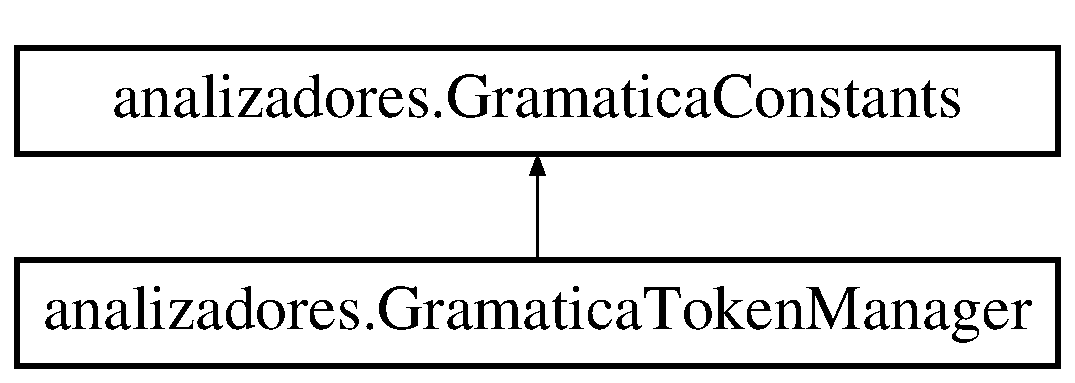
\includegraphics[height=2.000000cm]{classanalizadores_1_1_gramatica_token_manager}
\end{center}
\end{figure}
\subsection*{Public Member Functions}
\begin{DoxyCompactItemize}
\item 
void \mbox{\hyperlink{classanalizadores_1_1_gramatica_token_manager_a4dd7de62a7a2539af8844d147a128e74}{set\+Debug\+Stream}} (java.\+io.\+Print\+Stream ds)
\item 
\mbox{\hyperlink{classanalizadores_1_1_gramatica_token_manager_a6f39567296f646a754c87ca62cb7d78a}{Gramatica\+Token\+Manager}} (\mbox{\hyperlink{classanalizadores_1_1_simple_char_stream}{Simple\+Char\+Stream}} stream)
\item 
\mbox{\hyperlink{classanalizadores_1_1_gramatica_token_manager_a40bcd4b1673f1a37f1fac721ae154049}{Gramatica\+Token\+Manager}} (\mbox{\hyperlink{classanalizadores_1_1_simple_char_stream}{Simple\+Char\+Stream}} stream, int lex\+State)
\item 
void \mbox{\hyperlink{classanalizadores_1_1_gramatica_token_manager_a921966cc3d3430d9556f04cc4eddca0f}{Re\+Init}} (\mbox{\hyperlink{classanalizadores_1_1_simple_char_stream}{Simple\+Char\+Stream}} stream)
\item 
void \mbox{\hyperlink{classanalizadores_1_1_gramatica_token_manager_af95f8e720b5ee73b721aa490314ca933}{Re\+Init}} (\mbox{\hyperlink{classanalizadores_1_1_simple_char_stream}{Simple\+Char\+Stream}} stream, int lex\+State)
\item 
void \mbox{\hyperlink{classanalizadores_1_1_gramatica_token_manager_a8b938e445d55a0175957f9fce191581f}{Switch\+To}} (int lex\+State)
\item 
\mbox{\hyperlink{classanalizadores_1_1_token}{Token}} \mbox{\hyperlink{classanalizadores_1_1_gramatica_token_manager_a590a26d78e526ad8fa116390c45b7010}{get\+Next\+Token}} ()
\end{DoxyCompactItemize}
\subsection*{Public Attributes}
\begin{DoxyCompactItemize}
\item 
java.\+io.\+Print\+Stream \mbox{\hyperlink{classanalizadores_1_1_gramatica_token_manager_a2ec8c23d9151cea8cd5b1af72785fcb3}{debug\+Stream}} = System.\+out
\end{DoxyCompactItemize}
\subsection*{Static Public Attributes}
\begin{DoxyCompactItemize}
\item 
static final String \mbox{[}$\,$\mbox{]} \mbox{\hyperlink{classanalizadores_1_1_gramatica_token_manager_ae1c9e207113b8eb7137f51e9f536da24}{jjstr\+Literal\+Images}}
\item 
static final String \mbox{[}$\,$\mbox{]} \mbox{\hyperlink{classanalizadores_1_1_gramatica_token_manager_ab71dac104a1e700d4a241947012f31f4}{lex\+State\+Names}}
\item 
static final int \mbox{[}$\,$\mbox{]} \mbox{\hyperlink{classanalizadores_1_1_gramatica_token_manager_a2baa7049af1afa94f630c069005226db}{jjnew\+Lex\+State}}
\end{DoxyCompactItemize}
\subsection*{Protected Member Functions}
\begin{DoxyCompactItemize}
\item 
\mbox{\Hypertarget{classanalizadores_1_1_gramatica_token_manager_a66aa4d07660f6f1222bc56b2c95a5b07}\label{classanalizadores_1_1_gramatica_token_manager_a66aa4d07660f6f1222bc56b2c95a5b07}} 
\mbox{\hyperlink{classanalizadores_1_1_token}{Token}} {\bfseries jj\+Fill\+Token} ()
\end{DoxyCompactItemize}
\subsection*{Protected Attributes}
\begin{DoxyCompactItemize}
\item 
\mbox{\Hypertarget{classanalizadores_1_1_gramatica_token_manager_a599b2d374e33804e39ed44aeed378991}\label{classanalizadores_1_1_gramatica_token_manager_a599b2d374e33804e39ed44aeed378991}} 
\mbox{\hyperlink{classanalizadores_1_1_simple_char_stream}{Simple\+Char\+Stream}} {\bfseries input\+\_\+stream}
\item 
\mbox{\Hypertarget{classanalizadores_1_1_gramatica_token_manager_a146b9520c114189d732e4c0891b511be}\label{classanalizadores_1_1_gramatica_token_manager_a146b9520c114189d732e4c0891b511be}} 
char {\bfseries cur\+Char}
\end{DoxyCompactItemize}


\subsection{Detailed Description}
\mbox{\hyperlink{classanalizadores_1_1_token}{Token}} Manager. 

\subsection{Constructor \& Destructor Documentation}
\mbox{\Hypertarget{classanalizadores_1_1_gramatica_token_manager_a6f39567296f646a754c87ca62cb7d78a}\label{classanalizadores_1_1_gramatica_token_manager_a6f39567296f646a754c87ca62cb7d78a}} 
\index{analizadores\+::\+Gramatica\+Token\+Manager@{analizadores\+::\+Gramatica\+Token\+Manager}!Gramatica\+Token\+Manager@{Gramatica\+Token\+Manager}}
\index{Gramatica\+Token\+Manager@{Gramatica\+Token\+Manager}!analizadores\+::\+Gramatica\+Token\+Manager@{analizadores\+::\+Gramatica\+Token\+Manager}}
\subsubsection{\texorpdfstring{Gramatica\+Token\+Manager()}{GramaticaTokenManager()}\hspace{0.1cm}{\footnotesize\ttfamily [1/2]}}
{\footnotesize\ttfamily analizadores.\+Gramatica\+Token\+Manager.\+Gramatica\+Token\+Manager (\begin{DoxyParamCaption}\item[{\mbox{\hyperlink{classanalizadores_1_1_simple_char_stream}{Simple\+Char\+Stream}}}]{stream }\end{DoxyParamCaption})}

Constructor. \mbox{\Hypertarget{classanalizadores_1_1_gramatica_token_manager_a40bcd4b1673f1a37f1fac721ae154049}\label{classanalizadores_1_1_gramatica_token_manager_a40bcd4b1673f1a37f1fac721ae154049}} 
\index{analizadores\+::\+Gramatica\+Token\+Manager@{analizadores\+::\+Gramatica\+Token\+Manager}!Gramatica\+Token\+Manager@{Gramatica\+Token\+Manager}}
\index{Gramatica\+Token\+Manager@{Gramatica\+Token\+Manager}!analizadores\+::\+Gramatica\+Token\+Manager@{analizadores\+::\+Gramatica\+Token\+Manager}}
\subsubsection{\texorpdfstring{Gramatica\+Token\+Manager()}{GramaticaTokenManager()}\hspace{0.1cm}{\footnotesize\ttfamily [2/2]}}
{\footnotesize\ttfamily analizadores.\+Gramatica\+Token\+Manager.\+Gramatica\+Token\+Manager (\begin{DoxyParamCaption}\item[{\mbox{\hyperlink{classanalizadores_1_1_simple_char_stream}{Simple\+Char\+Stream}}}]{stream,  }\item[{int}]{lex\+State }\end{DoxyParamCaption})}

Constructor. 

\subsection{Member Function Documentation}
\mbox{\Hypertarget{classanalizadores_1_1_gramatica_token_manager_a590a26d78e526ad8fa116390c45b7010}\label{classanalizadores_1_1_gramatica_token_manager_a590a26d78e526ad8fa116390c45b7010}} 
\index{analizadores\+::\+Gramatica\+Token\+Manager@{analizadores\+::\+Gramatica\+Token\+Manager}!get\+Next\+Token@{get\+Next\+Token}}
\index{get\+Next\+Token@{get\+Next\+Token}!analizadores\+::\+Gramatica\+Token\+Manager@{analizadores\+::\+Gramatica\+Token\+Manager}}
\subsubsection{\texorpdfstring{get\+Next\+Token()}{getNextToken()}}
{\footnotesize\ttfamily \mbox{\hyperlink{classanalizadores_1_1_token}{Token}} analizadores.\+Gramatica\+Token\+Manager.\+get\+Next\+Token (\begin{DoxyParamCaption}{ }\end{DoxyParamCaption})}

Get the next \mbox{\hyperlink{classanalizadores_1_1_token}{Token}}. \mbox{\Hypertarget{classanalizadores_1_1_gramatica_token_manager_a921966cc3d3430d9556f04cc4eddca0f}\label{classanalizadores_1_1_gramatica_token_manager_a921966cc3d3430d9556f04cc4eddca0f}} 
\index{analizadores\+::\+Gramatica\+Token\+Manager@{analizadores\+::\+Gramatica\+Token\+Manager}!Re\+Init@{Re\+Init}}
\index{Re\+Init@{Re\+Init}!analizadores\+::\+Gramatica\+Token\+Manager@{analizadores\+::\+Gramatica\+Token\+Manager}}
\subsubsection{\texorpdfstring{Re\+Init()}{ReInit()}\hspace{0.1cm}{\footnotesize\ttfamily [1/2]}}
{\footnotesize\ttfamily void analizadores.\+Gramatica\+Token\+Manager.\+Re\+Init (\begin{DoxyParamCaption}\item[{\mbox{\hyperlink{classanalizadores_1_1_simple_char_stream}{Simple\+Char\+Stream}}}]{stream }\end{DoxyParamCaption})}

Reinitialise parser. \mbox{\Hypertarget{classanalizadores_1_1_gramatica_token_manager_af95f8e720b5ee73b721aa490314ca933}\label{classanalizadores_1_1_gramatica_token_manager_af95f8e720b5ee73b721aa490314ca933}} 
\index{analizadores\+::\+Gramatica\+Token\+Manager@{analizadores\+::\+Gramatica\+Token\+Manager}!Re\+Init@{Re\+Init}}
\index{Re\+Init@{Re\+Init}!analizadores\+::\+Gramatica\+Token\+Manager@{analizadores\+::\+Gramatica\+Token\+Manager}}
\subsubsection{\texorpdfstring{Re\+Init()}{ReInit()}\hspace{0.1cm}{\footnotesize\ttfamily [2/2]}}
{\footnotesize\ttfamily void analizadores.\+Gramatica\+Token\+Manager.\+Re\+Init (\begin{DoxyParamCaption}\item[{\mbox{\hyperlink{classanalizadores_1_1_simple_char_stream}{Simple\+Char\+Stream}}}]{stream,  }\item[{int}]{lex\+State }\end{DoxyParamCaption})}

Reinitialise parser. \mbox{\Hypertarget{classanalizadores_1_1_gramatica_token_manager_a4dd7de62a7a2539af8844d147a128e74}\label{classanalizadores_1_1_gramatica_token_manager_a4dd7de62a7a2539af8844d147a128e74}} 
\index{analizadores\+::\+Gramatica\+Token\+Manager@{analizadores\+::\+Gramatica\+Token\+Manager}!set\+Debug\+Stream@{set\+Debug\+Stream}}
\index{set\+Debug\+Stream@{set\+Debug\+Stream}!analizadores\+::\+Gramatica\+Token\+Manager@{analizadores\+::\+Gramatica\+Token\+Manager}}
\subsubsection{\texorpdfstring{set\+Debug\+Stream()}{setDebugStream()}}
{\footnotesize\ttfamily void analizadores.\+Gramatica\+Token\+Manager.\+set\+Debug\+Stream (\begin{DoxyParamCaption}\item[{java.\+io.\+Print\+Stream}]{ds }\end{DoxyParamCaption})}

Set debug output. \mbox{\Hypertarget{classanalizadores_1_1_gramatica_token_manager_a8b938e445d55a0175957f9fce191581f}\label{classanalizadores_1_1_gramatica_token_manager_a8b938e445d55a0175957f9fce191581f}} 
\index{analizadores\+::\+Gramatica\+Token\+Manager@{analizadores\+::\+Gramatica\+Token\+Manager}!Switch\+To@{Switch\+To}}
\index{Switch\+To@{Switch\+To}!analizadores\+::\+Gramatica\+Token\+Manager@{analizadores\+::\+Gramatica\+Token\+Manager}}
\subsubsection{\texorpdfstring{Switch\+To()}{SwitchTo()}}
{\footnotesize\ttfamily void analizadores.\+Gramatica\+Token\+Manager.\+Switch\+To (\begin{DoxyParamCaption}\item[{int}]{lex\+State }\end{DoxyParamCaption})}

Switch to specified lex state. 

\subsection{Member Data Documentation}
\mbox{\Hypertarget{classanalizadores_1_1_gramatica_token_manager_a2ec8c23d9151cea8cd5b1af72785fcb3}\label{classanalizadores_1_1_gramatica_token_manager_a2ec8c23d9151cea8cd5b1af72785fcb3}} 
\index{analizadores\+::\+Gramatica\+Token\+Manager@{analizadores\+::\+Gramatica\+Token\+Manager}!debug\+Stream@{debug\+Stream}}
\index{debug\+Stream@{debug\+Stream}!analizadores\+::\+Gramatica\+Token\+Manager@{analizadores\+::\+Gramatica\+Token\+Manager}}
\subsubsection{\texorpdfstring{debug\+Stream}{debugStream}}
{\footnotesize\ttfamily java.\+io.\+Print\+Stream analizadores.\+Gramatica\+Token\+Manager.\+debug\+Stream = System.\+out}

Debug output. \mbox{\Hypertarget{classanalizadores_1_1_gramatica_token_manager_a2baa7049af1afa94f630c069005226db}\label{classanalizadores_1_1_gramatica_token_manager_a2baa7049af1afa94f630c069005226db}} 
\index{analizadores\+::\+Gramatica\+Token\+Manager@{analizadores\+::\+Gramatica\+Token\+Manager}!jjnew\+Lex\+State@{jjnew\+Lex\+State}}
\index{jjnew\+Lex\+State@{jjnew\+Lex\+State}!analizadores\+::\+Gramatica\+Token\+Manager@{analizadores\+::\+Gramatica\+Token\+Manager}}
\subsubsection{\texorpdfstring{jjnew\+Lex\+State}{jjnewLexState}}
{\footnotesize\ttfamily final int \mbox{[}$\,$\mbox{]} analizadores.\+Gramatica\+Token\+Manager.\+jjnew\+Lex\+State\hspace{0.3cm}{\ttfamily [static]}}

{\bfseries Initial value\+:}
\begin{DoxyCode}
= \{
   -1, -1, -1, -1, -1, -1, -1, -1, -1, -1, -1, -1, -1, -1, -1, -1, -1, -1, -1, -1, -1, -1, -1, -1, -1, 
   -1, -1, -1, -1, -1, -1, -1, -1, -1, -1, -1, -1, -1, -1, -1, -1, -1, -1, -1, 1, -1, -1, -1, -1, -1, 
   -1, -1, -1, 0, 
\}
\end{DoxyCode}
Lex State array. \mbox{\Hypertarget{classanalizadores_1_1_gramatica_token_manager_ae1c9e207113b8eb7137f51e9f536da24}\label{classanalizadores_1_1_gramatica_token_manager_ae1c9e207113b8eb7137f51e9f536da24}} 
\index{analizadores\+::\+Gramatica\+Token\+Manager@{analizadores\+::\+Gramatica\+Token\+Manager}!jjstr\+Literal\+Images@{jjstr\+Literal\+Images}}
\index{jjstr\+Literal\+Images@{jjstr\+Literal\+Images}!analizadores\+::\+Gramatica\+Token\+Manager@{analizadores\+::\+Gramatica\+Token\+Manager}}
\subsubsection{\texorpdfstring{jjstr\+Literal\+Images}{jjstrLiteralImages}}
{\footnotesize\ttfamily final String \mbox{[}$\,$\mbox{]} analizadores.\+Gramatica\+Token\+Manager.\+jjstr\+Literal\+Images\hspace{0.3cm}{\ttfamily [static]}}

{\bfseries Initial value\+:}
\begin{DoxyCode}
= \{
\textcolor{stringliteral}{""}, null, null, null, null, null, null, null, null, null, null, null, null, 
null, null, \textcolor{stringliteral}{"\(\backslash\)73"}, \textcolor{stringliteral}{"\(\backslash\)54"}, \textcolor{stringliteral}{"\(\backslash\)50"}, \textcolor{stringliteral}{"\(\backslash\)51"}, \textcolor{stringliteral}{"\(\backslash\)133"}, \textcolor{stringliteral}{"\(\backslash\)135"}, \textcolor{stringliteral}{"\(\backslash\)173"}, \textcolor{stringliteral}{"\(\backslash\)175"}, \textcolor{stringliteral}{"\(\backslash\)77"}, 
\textcolor{stringliteral}{"\(\backslash\)72"}, \textcolor{stringliteral}{"\(\backslash\)53"}, \textcolor{stringliteral}{"\(\backslash\)55"}, \textcolor{stringliteral}{"\(\backslash\)52"}, \textcolor{stringliteral}{"\(\backslash\)45\(\backslash\)45"}, \textcolor{stringliteral}{"\(\backslash\)57"}, \textcolor{stringliteral}{"\(\backslash\)136"}, \textcolor{stringliteral}{"\(\backslash\)75"}, \textcolor{stringliteral}{"\(\backslash\)74"}, \textcolor{stringliteral}{"\(\backslash\)76"}, \textcolor{stringliteral}{"\(\backslash\)74\(\backslash\)75"}, 
\textcolor{stringliteral}{"\(\backslash\)76\(\backslash\)75"}, \textcolor{stringliteral}{"\(\backslash\)75\(\backslash\)75"}, \textcolor{stringliteral}{"\(\backslash\)41\(\backslash\)75"}, \textcolor{stringliteral}{"\(\backslash\)46"}, \textcolor{stringliteral}{"\(\backslash\)174"}, \textcolor{stringliteral}{"\(\backslash\)41"}, null, null, null, null, null, null, 
null, null, null, null, null, null, null, \}
\end{DoxyCode}
\mbox{\hyperlink{classanalizadores_1_1_token}{Token}} literal values. \mbox{\Hypertarget{classanalizadores_1_1_gramatica_token_manager_ab71dac104a1e700d4a241947012f31f4}\label{classanalizadores_1_1_gramatica_token_manager_ab71dac104a1e700d4a241947012f31f4}} 
\index{analizadores\+::\+Gramatica\+Token\+Manager@{analizadores\+::\+Gramatica\+Token\+Manager}!lex\+State\+Names@{lex\+State\+Names}}
\index{lex\+State\+Names@{lex\+State\+Names}!analizadores\+::\+Gramatica\+Token\+Manager@{analizadores\+::\+Gramatica\+Token\+Manager}}
\subsubsection{\texorpdfstring{lex\+State\+Names}{lexStateNames}}
{\footnotesize\ttfamily final String \mbox{[}$\,$\mbox{]} analizadores.\+Gramatica\+Token\+Manager.\+lex\+State\+Names\hspace{0.3cm}{\ttfamily [static]}}

{\bfseries Initial value\+:}
\begin{DoxyCode}
= \{
   \textcolor{stringliteral}{"DEFAULT"}, 
   \textcolor{stringliteral}{"STRING\_STATE"}, 
\}
\end{DoxyCode}
Lexer state names. 

The documentation for this class was generated from the following file\+:\begin{DoxyCompactItemize}
\item 
src/analizadores/Gramatica\+Token\+Manager.\+java\end{DoxyCompactItemize}

\hypertarget{classast_1_1expresiones_1_1_identificador}{}\section{ast.\+expresiones.\+Identificador Class Reference}
\label{classast_1_1expresiones_1_1_identificador}\index{ast.\+expresiones.\+Identificador@{ast.\+expresiones.\+Identificador}}
Inheritance diagram for ast.\+expresiones.\+Identificador\+:\begin{figure}[H]
\begin{center}
\leavevmode
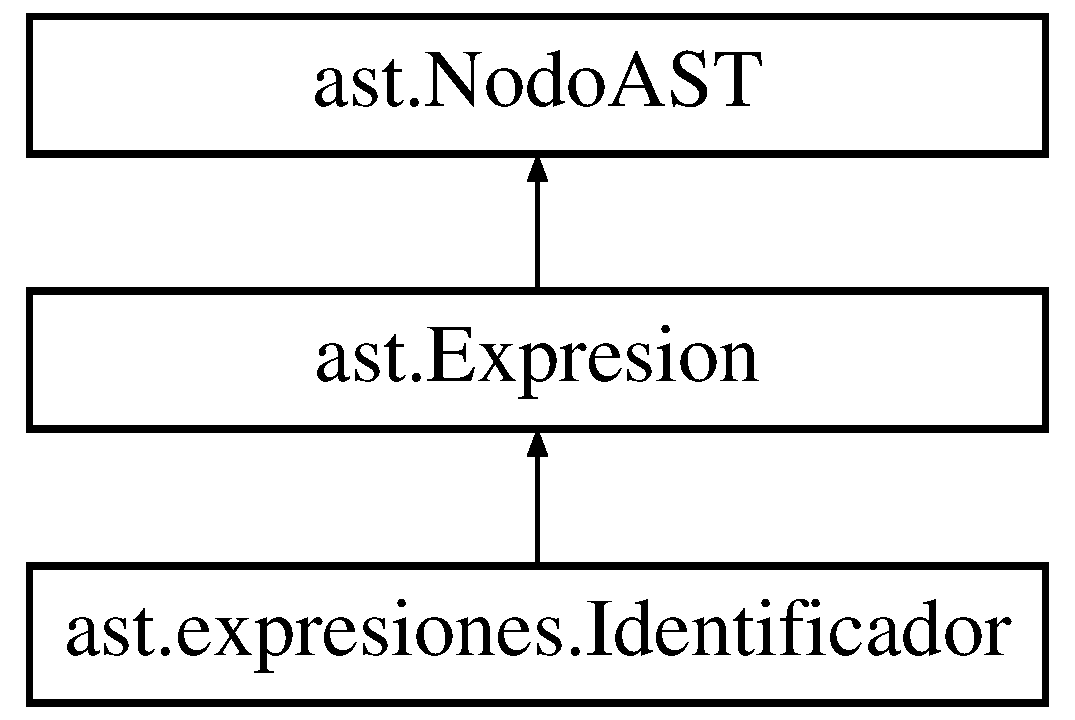
\includegraphics[height=3.000000cm]{classast_1_1expresiones_1_1_identificador}
\end{center}
\end{figure}
\subsection*{Public Member Functions}
\begin{DoxyCompactItemize}
\item 
\mbox{\Hypertarget{classast_1_1expresiones_1_1_identificador_ab35b2c54733b35e02d6a3172796aae5b}\label{classast_1_1expresiones_1_1_identificador_ab35b2c54733b35e02d6a3172796aae5b}} 
{\bfseries Identificador} (String val, int linea, int col, boolean is\+Assign)
\item 
\mbox{\Hypertarget{classast_1_1expresiones_1_1_identificador_a12a41c653049188119a77e6ed03b8d20}\label{classast_1_1expresiones_1_1_identificador_a12a41c653049188119a77e6ed03b8d20}} 
{\bfseries Identificador} (String val, Linked\+List$<$ \mbox{\hyperlink{classentorno_1_1nodo_exp}{nodo\+Exp}} $>$ lista, boolean is\+Assign, int linea, int col)
\item 
\mbox{\Hypertarget{classast_1_1expresiones_1_1_identificador_a21e953d172a1343dc7c8057c597cad67}\label{classast_1_1expresiones_1_1_identificador_a21e953d172a1343dc7c8057c597cad67}} 
\mbox{\hyperlink{classentorno_1_1_tipo}{Tipo}} {\bfseries get\+Tipo} (\mbox{\hyperlink{classentorno_1_1_entorno}{Entorno}} ent)
\item 
\mbox{\Hypertarget{classast_1_1expresiones_1_1_identificador_abe016822639c1e988f2ff989467b8907}\label{classast_1_1expresiones_1_1_identificador_abe016822639c1e988f2ff989467b8907}} 
Object {\bfseries get\+Valor\+Implicito} (\mbox{\hyperlink{classentorno_1_1_entorno}{Entorno}} ent)
\item 
\mbox{\Hypertarget{classast_1_1expresiones_1_1_identificador_a9d43f250c69d1c685fb26ca496c55880}\label{classast_1_1expresiones_1_1_identificador_a9d43f250c69d1c685fb26ca496c55880}} 
int {\bfseries linea} ()
\item 
\mbox{\Hypertarget{classast_1_1expresiones_1_1_identificador_a00cc3e1ec5c836c7aca530c3a26f4807}\label{classast_1_1expresiones_1_1_identificador_a00cc3e1ec5c836c7aca530c3a26f4807}} 
int {\bfseries columna} ()
\item 
\mbox{\Hypertarget{classast_1_1expresiones_1_1_identificador_ae1e89a9747cd5668df0751e3e58d10ca}\label{classast_1_1expresiones_1_1_identificador_ae1e89a9747cd5668df0751e3e58d10ca}} 
String {\bfseries get\+Val} ()
\item 
\mbox{\Hypertarget{classast_1_1expresiones_1_1_identificador_aeb1ee3da3a5be1f0438acd943af1f882}\label{classast_1_1expresiones_1_1_identificador_aeb1ee3da3a5be1f0438acd943af1f882}} 
void {\bfseries set\+Val} (String val)
\item 
\mbox{\Hypertarget{classast_1_1expresiones_1_1_identificador_a72f16a7d91e176d300e6576c83cd5861}\label{classast_1_1expresiones_1_1_identificador_a72f16a7d91e176d300e6576c83cd5861}} 
Linked\+List$<$ \mbox{\hyperlink{classentorno_1_1nodo_exp}{nodo\+Exp}} $>$ {\bfseries get\+Lista} ()
\item 
\mbox{\Hypertarget{classast_1_1expresiones_1_1_identificador_a1e72daab88a2caf01fa5767e0c69f2cb}\label{classast_1_1expresiones_1_1_identificador_a1e72daab88a2caf01fa5767e0c69f2cb}} 
void {\bfseries set\+Lista} (Linked\+List$<$ \mbox{\hyperlink{classentorno_1_1nodo_exp}{nodo\+Exp}} $>$ lista)
\item 
\mbox{\Hypertarget{classast_1_1expresiones_1_1_identificador_a233276fbee95cffe1c3aa289b708530a}\label{classast_1_1expresiones_1_1_identificador_a233276fbee95cffe1c3aa289b708530a}} 
int {\bfseries get\+Linea} ()
\item 
\mbox{\Hypertarget{classast_1_1expresiones_1_1_identificador_ae1f07dd6c7503b90861e4798040ac5b5}\label{classast_1_1expresiones_1_1_identificador_ae1f07dd6c7503b90861e4798040ac5b5}} 
void {\bfseries set\+Linea} (int linea)
\item 
\mbox{\Hypertarget{classast_1_1expresiones_1_1_identificador_a13e816233ee376ce7119afd12c12eda7}\label{classast_1_1expresiones_1_1_identificador_a13e816233ee376ce7119afd12c12eda7}} 
int {\bfseries get\+Col} ()
\item 
\mbox{\Hypertarget{classast_1_1expresiones_1_1_identificador_aad40acb7bfbb0f58288cbe1fa0d19b5e}\label{classast_1_1expresiones_1_1_identificador_aad40acb7bfbb0f58288cbe1fa0d19b5e}} 
void {\bfseries set\+Col} (int col)
\item 
\mbox{\Hypertarget{classast_1_1expresiones_1_1_identificador_a2b74b064eb3446b2e1d943cb9fe65f6c}\label{classast_1_1expresiones_1_1_identificador_a2b74b064eb3446b2e1d943cb9fe65f6c}} 
boolean {\bfseries is\+Is\+Assign} ()
\item 
\mbox{\Hypertarget{classast_1_1expresiones_1_1_identificador_a60cefaa05521398043b79001f6db2753}\label{classast_1_1expresiones_1_1_identificador_a60cefaa05521398043b79001f6db2753}} 
void {\bfseries set\+Is\+Assign} (boolean is\+Assign)
\item 
\mbox{\Hypertarget{classast_1_1expresiones_1_1_identificador_a7be778d7639474fe59d9db1614f4bb1b}\label{classast_1_1expresiones_1_1_identificador_a7be778d7639474fe59d9db1614f4bb1b}} 
String {\bfseries get\+Nombre} (String\+Builder builder, String parent, int cont)
\end{DoxyCompactItemize}


\subsection{Detailed Description}
\begin{DoxyAuthor}{Author}
p\+\_\+ab1 
\end{DoxyAuthor}


The documentation for this class was generated from the following file\+:\begin{DoxyCompactItemize}
\item 
src/ast/expresiones/Identificador.\+java\end{DoxyCompactItemize}

\hypertarget{classast_1_1instrucciones_1_1_if}{}\section{ast.\+instrucciones.\+If Class Reference}
\label{classast_1_1instrucciones_1_1_if}\index{ast.\+instrucciones.\+If@{ast.\+instrucciones.\+If}}
Inheritance diagram for ast.\+instrucciones.\+If\+:\begin{figure}[H]
\begin{center}
\leavevmode
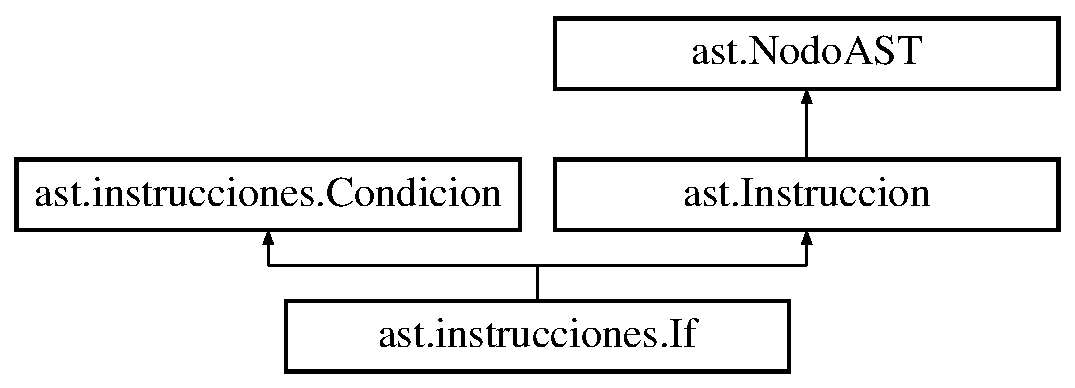
\includegraphics[height=3.000000cm]{classast_1_1instrucciones_1_1_if}
\end{center}
\end{figure}
\subsection*{Public Member Functions}
\begin{DoxyCompactItemize}
\item 
\mbox{\Hypertarget{classast_1_1instrucciones_1_1_if_a0f89e733a56b9787330354e01f3bafe0}\label{classast_1_1instrucciones_1_1_if_a0f89e733a56b9787330354e01f3bafe0}} 
{\bfseries If} (Linked\+List$<$ \mbox{\hyperlink{interfaceast_1_1_nodo_a_s_t}{Nodo\+A\+ST}} $>$ ins, \mbox{\hyperlink{interfaceast_1_1_expresion}{Expresion}} cond, int linea)
\item 
\mbox{\Hypertarget{classast_1_1instrucciones_1_1_if_abc8fbc61b74acdd8cfab0a57d910543b}\label{classast_1_1instrucciones_1_1_if_abc8fbc61b74acdd8cfab0a57d910543b}} 
{\bfseries If} (Linked\+List$<$ \mbox{\hyperlink{interfaceast_1_1_nodo_a_s_t}{Nodo\+A\+ST}} $>$ ins, \mbox{\hyperlink{interfaceast_1_1_expresion}{Expresion}} cond, Linked\+List$<$ \mbox{\hyperlink{interfaceast_1_1_nodo_a_s_t}{Nodo\+A\+ST}} $>$ins\+Else, int linea)
\item 
\mbox{\Hypertarget{classast_1_1instrucciones_1_1_if_a4e64435ce4409ec289516aca9395481e}\label{classast_1_1instrucciones_1_1_if_a4e64435ce4409ec289516aca9395481e}} 
{\bfseries If} (Linked\+List$<$ \mbox{\hyperlink{interfaceast_1_1_nodo_a_s_t}{Nodo\+A\+ST}} $>$ ins, \mbox{\hyperlink{interfaceast_1_1_expresion}{Expresion}} cond, \mbox{\hyperlink{interfaceast_1_1_instruccion}{Instruccion}} else\+If, int linea)
\item 
\mbox{\Hypertarget{classast_1_1instrucciones_1_1_if_ad3e7a5d5eb42a040eac6bbee48fd5787}\label{classast_1_1instrucciones_1_1_if_ad3e7a5d5eb42a040eac6bbee48fd5787}} 
Object {\bfseries ejecutar} (\mbox{\hyperlink{classentorno_1_1_entorno}{Entorno}} ent)
\item 
\mbox{\Hypertarget{classast_1_1instrucciones_1_1_if_a63270d2ecde32b73162cafc6a3075fc3}\label{classast_1_1instrucciones_1_1_if_a63270d2ecde32b73162cafc6a3075fc3}} 
int {\bfseries linea} ()
\item 
\mbox{\Hypertarget{classast_1_1instrucciones_1_1_if_aa08a9dcc80ca866b10209f792ddd7bc1}\label{classast_1_1instrucciones_1_1_if_aa08a9dcc80ca866b10209f792ddd7bc1}} 
int {\bfseries columna} ()
\item 
\mbox{\Hypertarget{classast_1_1instrucciones_1_1_if_aa80fea499762ab1ec22628d43f04a0c8}\label{classast_1_1instrucciones_1_1_if_aa80fea499762ab1ec22628d43f04a0c8}} 
String {\bfseries get\+Nombre} (String\+Builder builder, String parent, int cont)
\item 
\mbox{\Hypertarget{classast_1_1instrucciones_1_1_if_a0ecf379dfcb3bbed21c509237b27e084}\label{classast_1_1instrucciones_1_1_if_a0ecf379dfcb3bbed21c509237b27e084}} 
Linked\+List$<$ \mbox{\hyperlink{interfaceast_1_1_nodo_a_s_t}{Nodo\+A\+ST}} $>$ {\bfseries get\+Ins\+Else} ()
\end{DoxyCompactItemize}


\subsection{Detailed Description}
\begin{DoxyAuthor}{Author}
p\+\_\+ab1 
\end{DoxyAuthor}


The documentation for this class was generated from the following file\+:\begin{DoxyCompactItemize}
\item 
src/ast/instrucciones/If.\+java\end{DoxyCompactItemize}

\hypertarget{interfaceast_1_1_instruccion}{}\section{ast.\+Instruccion Interface Reference}
\label{interfaceast_1_1_instruccion}\index{ast.\+Instruccion@{ast.\+Instruccion}}
Inheritance diagram for ast.\+Instruccion\+:\begin{figure}[H]
\begin{center}
\leavevmode
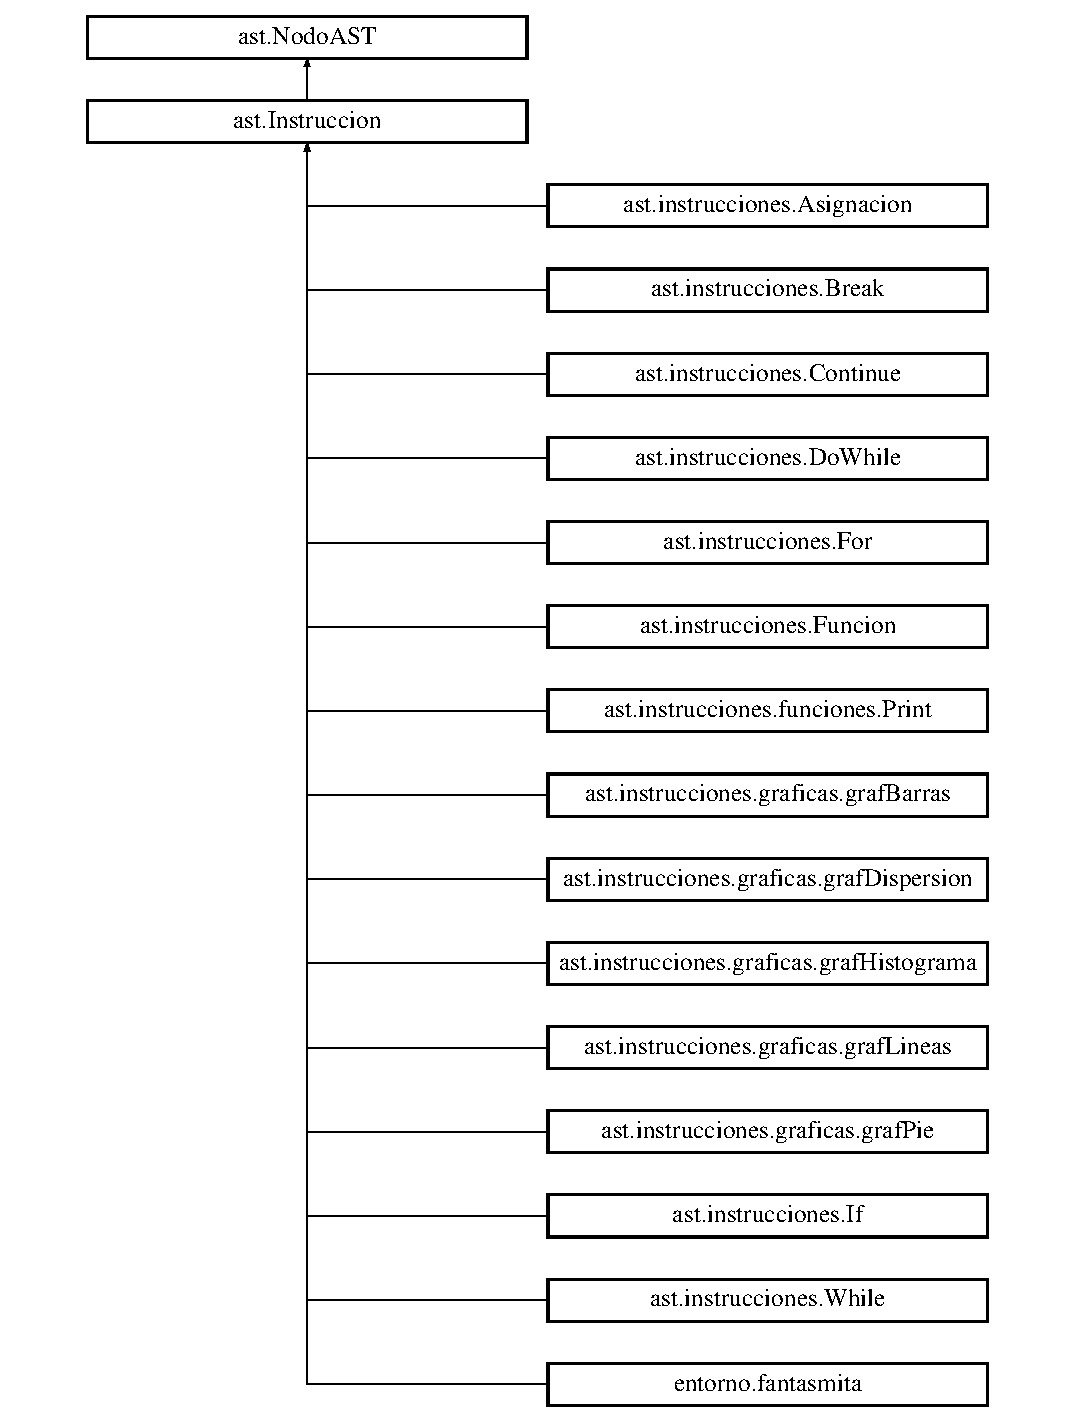
\includegraphics[height=12.000000cm]{interfaceast_1_1_instruccion}
\end{center}
\end{figure}
\subsection*{Public Member Functions}
\begin{DoxyCompactItemize}
\item 
\mbox{\Hypertarget{interfaceast_1_1_instruccion_a2c794ecf93e49743324d82b3ddb1fe89}\label{interfaceast_1_1_instruccion_a2c794ecf93e49743324d82b3ddb1fe89}} 
Object {\bfseries ejecutar} (\mbox{\hyperlink{classentorno_1_1_entorno}{Entorno}} ent)
\end{DoxyCompactItemize}


\subsection{Detailed Description}
\begin{DoxyAuthor}{Author}
p\+\_\+ab1 
\end{DoxyAuthor}


The documentation for this interface was generated from the following file\+:\begin{DoxyCompactItemize}
\item 
src/ast/Instruccion.\+java\end{DoxyCompactItemize}

\hypertarget{classolc2_1_1p1__201504242_1_1_j_error}{}\section{olc2.\+p1\+\_\+201504242.\+J\+Error Class Reference}
\label{classolc2_1_1p1__201504242_1_1_j_error}\index{olc2.\+p1\+\_\+201504242.\+J\+Error@{olc2.\+p1\+\_\+201504242.\+J\+Error}}
\subsection*{Public Member Functions}
\begin{DoxyCompactItemize}
\item 
\mbox{\Hypertarget{classolc2_1_1p1__201504242_1_1_j_error_a4903663b02145da13646cff7044e883c}\label{classolc2_1_1p1__201504242_1_1_j_error_a4903663b02145da13646cff7044e883c}} 
{\bfseries J\+Error} (String tipo\+Error, int linea, int columna, String desc)
\item 
\mbox{\Hypertarget{classolc2_1_1p1__201504242_1_1_j_error_a955d0b2ad6b278522be4aa098c6bf743}\label{classolc2_1_1p1__201504242_1_1_j_error_a955d0b2ad6b278522be4aa098c6bf743}} 
String {\bfseries get\+Tipo\+Error} ()
\item 
\mbox{\Hypertarget{classolc2_1_1p1__201504242_1_1_j_error_a264576d9bef73dc703eda986a3655d3a}\label{classolc2_1_1p1__201504242_1_1_j_error_a264576d9bef73dc703eda986a3655d3a}} 
void {\bfseries set\+Tipo\+Error} (String tipo\+Error)
\item 
\mbox{\Hypertarget{classolc2_1_1p1__201504242_1_1_j_error_a65cf04e0575990431de411d523edab64}\label{classolc2_1_1p1__201504242_1_1_j_error_a65cf04e0575990431de411d523edab64}} 
int {\bfseries get\+Linea} ()
\item 
\mbox{\Hypertarget{classolc2_1_1p1__201504242_1_1_j_error_a6ff5511f1825dbb15e3447c310183dac}\label{classolc2_1_1p1__201504242_1_1_j_error_a6ff5511f1825dbb15e3447c310183dac}} 
void {\bfseries set\+Linea} (int linea)
\item 
\mbox{\Hypertarget{classolc2_1_1p1__201504242_1_1_j_error_a644b16409ee68752bed37318d8c1cbbf}\label{classolc2_1_1p1__201504242_1_1_j_error_a644b16409ee68752bed37318d8c1cbbf}} 
int {\bfseries get\+Columna} ()
\item 
\mbox{\Hypertarget{classolc2_1_1p1__201504242_1_1_j_error_a02ca8c5018a5e41befed94aa273d302f}\label{classolc2_1_1p1__201504242_1_1_j_error_a02ca8c5018a5e41befed94aa273d302f}} 
void {\bfseries set\+Columna} (int columna)
\item 
\mbox{\Hypertarget{classolc2_1_1p1__201504242_1_1_j_error_aa63dcf0cc471aaba81f26104936c32e4}\label{classolc2_1_1p1__201504242_1_1_j_error_aa63dcf0cc471aaba81f26104936c32e4}} 
String {\bfseries get\+Desc} ()
\item 
\mbox{\Hypertarget{classolc2_1_1p1__201504242_1_1_j_error_af5285d0604a52631ebd3f0383d3aa120}\label{classolc2_1_1p1__201504242_1_1_j_error_af5285d0604a52631ebd3f0383d3aa120}} 
void {\bfseries set\+Desc} (String desc)
\end{DoxyCompactItemize}


\subsection{Detailed Description}
\begin{DoxyAuthor}{Author}
p\+\_\+ab1 
\end{DoxyAuthor}


The documentation for this class was generated from the following file\+:\begin{DoxyCompactItemize}
\item 
src/olc2/p1\+\_\+201504242/J\+Error.\+java\end{DoxyCompactItemize}

\hypertarget{classast_1_1instrucciones_1_1funciones_1_1_length}{}\section{ast.\+instrucciones.\+funciones.\+Length Class Reference}
\label{classast_1_1instrucciones_1_1funciones_1_1_length}\index{ast.\+instrucciones.\+funciones.\+Length@{ast.\+instrucciones.\+funciones.\+Length}}
Inheritance diagram for ast.\+instrucciones.\+funciones.\+Length\+:\begin{figure}[H]
\begin{center}
\leavevmode
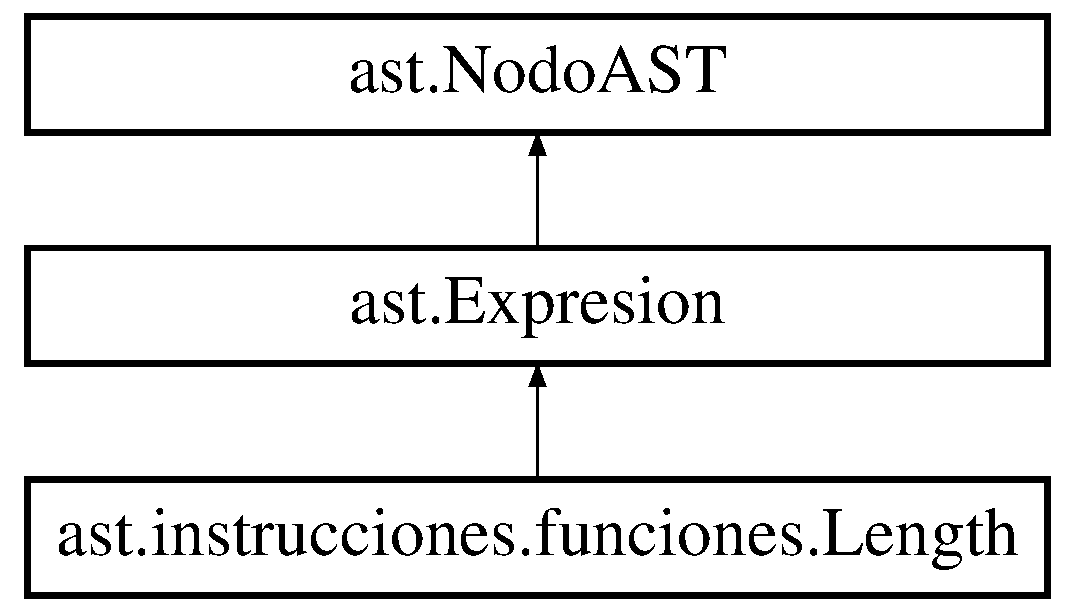
\includegraphics[height=3.000000cm]{classast_1_1instrucciones_1_1funciones_1_1_length}
\end{center}
\end{figure}
\subsection*{Public Member Functions}
\begin{DoxyCompactItemize}
\item 
\mbox{\Hypertarget{classast_1_1instrucciones_1_1funciones_1_1_length_aa2acc25f4924ede4aa6b2d315496baae}\label{classast_1_1instrucciones_1_1funciones_1_1_length_aa2acc25f4924ede4aa6b2d315496baae}} 
{\bfseries Length} (Linked\+List$<$ \mbox{\hyperlink{interfaceast_1_1_nodo_a_s_t}{Nodo\+A\+ST}} $>$ valor, int linea, int col)
\item 
\mbox{\Hypertarget{classast_1_1instrucciones_1_1funciones_1_1_length_ac0d711d436782df361d1ac85f91bf7fd}\label{classast_1_1instrucciones_1_1funciones_1_1_length_ac0d711d436782df361d1ac85f91bf7fd}} 
\mbox{\hyperlink{classentorno_1_1_tipo}{Tipo}} {\bfseries get\+Tipo} (\mbox{\hyperlink{classentorno_1_1_entorno}{Entorno}} ent)
\item 
\mbox{\Hypertarget{classast_1_1instrucciones_1_1funciones_1_1_length_a406a8ee9778dd07d054d65ee8e044a5f}\label{classast_1_1instrucciones_1_1funciones_1_1_length_a406a8ee9778dd07d054d65ee8e044a5f}} 
Object {\bfseries get\+Valor\+Implicito} (\mbox{\hyperlink{classentorno_1_1_entorno}{Entorno}} ent)
\item 
\mbox{\Hypertarget{classast_1_1instrucciones_1_1funciones_1_1_length_a46fb440694a43e3a53464c28c4ff9e4b}\label{classast_1_1instrucciones_1_1funciones_1_1_length_a46fb440694a43e3a53464c28c4ff9e4b}} 
int {\bfseries linea} ()
\item 
\mbox{\Hypertarget{classast_1_1instrucciones_1_1funciones_1_1_length_a8a9597fd6ea4786aeefba4976a8b62e7}\label{classast_1_1instrucciones_1_1funciones_1_1_length_a8a9597fd6ea4786aeefba4976a8b62e7}} 
int {\bfseries columna} ()
\item 
\mbox{\Hypertarget{classast_1_1instrucciones_1_1funciones_1_1_length_a5ac2bc119702f390692eb86307e04b4e}\label{classast_1_1instrucciones_1_1funciones_1_1_length_a5ac2bc119702f390692eb86307e04b4e}} 
String {\bfseries get\+Nombre} (String\+Builder builder, String parent, int cont)
\end{DoxyCompactItemize}


\subsection{Detailed Description}
\begin{DoxyAuthor}{Author}
p\+\_\+ab1 
\end{DoxyAuthor}


The documentation for this class was generated from the following file\+:\begin{DoxyCompactItemize}
\item 
src/ast/instrucciones/funciones/Length.\+java\end{DoxyCompactItemize}

\hypertarget{classanalizadores_1_1_lexico}{}\section{analizadores.\+Lexico Class Reference}
\label{classanalizadores_1_1_lexico}\index{analizadores.\+Lexico@{analizadores.\+Lexico}}
Inheritance diagram for analizadores.\+Lexico\+:\begin{figure}[H]
\begin{center}
\leavevmode
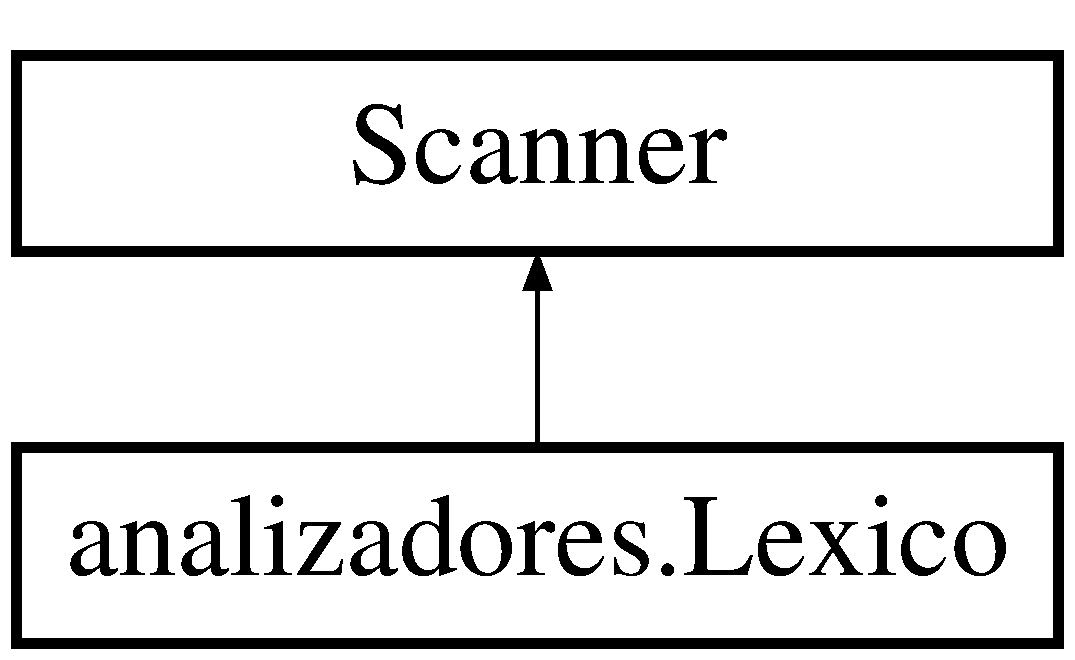
\includegraphics[height=2.000000cm]{classanalizadores_1_1_lexico}
\end{center}
\end{figure}
\subsection*{Public Member Functions}
\begin{DoxyCompactItemize}
\item 
\mbox{\Hypertarget{classanalizadores_1_1_lexico_ad64fd671966c3991545ef5a6a212cb9d}\label{classanalizadores_1_1_lexico_ad64fd671966c3991545ef5a6a212cb9d}} 
{\bfseries Lexico} (java.\+io.\+Reader reader)
\item 
\mbox{\Hypertarget{classanalizadores_1_1_lexico_a45236ae2e7893b61f7de9df2f3dde79d}\label{classanalizadores_1_1_lexico_a45236ae2e7893b61f7de9df2f3dde79d}} 
{\bfseries Lexico} (java.\+io.\+Input\+Stream instream)
\item 
\mbox{\Hypertarget{classanalizadores_1_1_lexico_a024e816fa3941af9cb6e890bb1fb6e3c}\label{classanalizadores_1_1_lexico_a024e816fa3941af9cb6e890bb1fb6e3c}} 
java\+\_\+cup.\+runtime.\+Symbol {\bfseries next\+\_\+token} ()  throws java.\+io.\+I\+O\+Exception 
\end{DoxyCompactItemize}


The documentation for this class was generated from the following file\+:\begin{DoxyCompactItemize}
\item 
src/analizadores/Lexico.\+java\end{DoxyCompactItemize}

\hypertarget{classast_1_1instrucciones_1_1funciones_1_1_list_var}{}\section{ast.\+instrucciones.\+funciones.\+List\+Var Class Reference}
\label{classast_1_1instrucciones_1_1funciones_1_1_list_var}\index{ast.\+instrucciones.\+funciones.\+List\+Var@{ast.\+instrucciones.\+funciones.\+List\+Var}}
Inheritance diagram for ast.\+instrucciones.\+funciones.\+List\+Var\+:\begin{figure}[H]
\begin{center}
\leavevmode
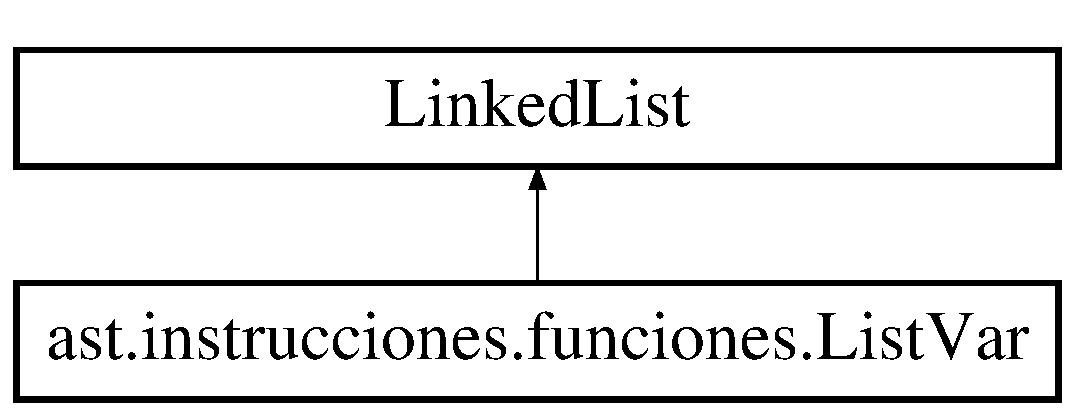
\includegraphics[height=2.000000cm]{classast_1_1instrucciones_1_1funciones_1_1_list_var}
\end{center}
\end{figure}
\subsection*{Public Member Functions}
\begin{DoxyCompactItemize}
\item 
\mbox{\Hypertarget{classast_1_1instrucciones_1_1funciones_1_1_list_var_ab0e6a2e87a44a4cba29be32fb1b7de05}\label{classast_1_1instrucciones_1_1funciones_1_1_list_var_ab0e6a2e87a44a4cba29be32fb1b7de05}} 
void {\bfseries add} (int i, Object e)
\item 
\mbox{\Hypertarget{classast_1_1instrucciones_1_1funciones_1_1_list_var_afc6bf4368bef6a8101497544f6f54446}\label{classast_1_1instrucciones_1_1funciones_1_1_list_var_afc6bf4368bef6a8101497544f6f54446}} 
Object {\bfseries get\+Assig} (int i)
\end{DoxyCompactItemize}


\subsection{Detailed Description}
\begin{DoxyAuthor}{Author}
p\+\_\+ab1 
\end{DoxyAuthor}


The documentation for this class was generated from the following file\+:\begin{DoxyCompactItemize}
\item 
src/ast/instrucciones/funciones/List\+Var.\+java\end{DoxyCompactItemize}

\hypertarget{classast_1_1expresiones_1_1_literal}{}\section{ast.\+expresiones.\+Literal Class Reference}
\label{classast_1_1expresiones_1_1_literal}\index{ast.\+expresiones.\+Literal@{ast.\+expresiones.\+Literal}}
Inheritance diagram for ast.\+expresiones.\+Literal\+:\begin{figure}[H]
\begin{center}
\leavevmode
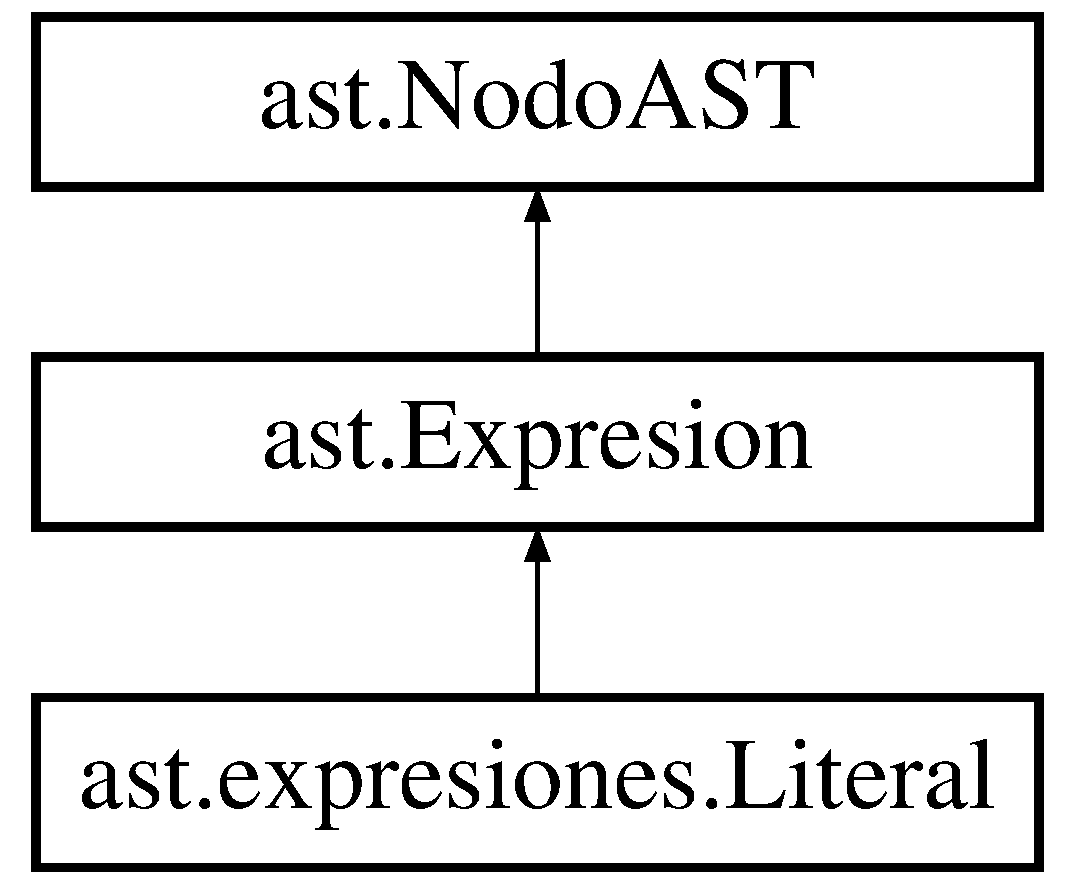
\includegraphics[height=3.000000cm]{classast_1_1expresiones_1_1_literal}
\end{center}
\end{figure}
\subsection*{Public Member Functions}
\begin{DoxyCompactItemize}
\item 
\mbox{\Hypertarget{classast_1_1expresiones_1_1_literal_a2fcbb0b170459a390c51e05897baf23b}\label{classast_1_1expresiones_1_1_literal_a2fcbb0b170459a390c51e05897baf23b}} 
{\bfseries Literal} (Object valor, \mbox{\hyperlink{classentorno_1_1_tipo}{Tipo}} tipo, int linea, int col)
\item 
\mbox{\Hypertarget{classast_1_1expresiones_1_1_literal_aeffa28d139800b7d2b2394c0574b6e7f}\label{classast_1_1expresiones_1_1_literal_aeffa28d139800b7d2b2394c0574b6e7f}} 
\mbox{\hyperlink{classentorno_1_1_tipo}{Tipo}} {\bfseries get\+Tipo} (\mbox{\hyperlink{classentorno_1_1_entorno}{Entorno}} ent)
\item 
\mbox{\Hypertarget{classast_1_1expresiones_1_1_literal_ac8f5dd86017ba8f623d2b87a1259c53a}\label{classast_1_1expresiones_1_1_literal_ac8f5dd86017ba8f623d2b87a1259c53a}} 
Object {\bfseries get\+Valor\+Implicito} (\mbox{\hyperlink{classentorno_1_1_entorno}{Entorno}} ent)
\item 
\mbox{\Hypertarget{classast_1_1expresiones_1_1_literal_abeccef2c29fe321ebbf4612a985ffaaa}\label{classast_1_1expresiones_1_1_literal_abeccef2c29fe321ebbf4612a985ffaaa}} 
int {\bfseries linea} ()
\item 
\mbox{\Hypertarget{classast_1_1expresiones_1_1_literal_ab8acaa47d4363d6409252fdf4e2b82b2}\label{classast_1_1expresiones_1_1_literal_ab8acaa47d4363d6409252fdf4e2b82b2}} 
int {\bfseries columna} ()
\item 
\mbox{\Hypertarget{classast_1_1expresiones_1_1_literal_a31fa9639be621619514a8cce14347c72}\label{classast_1_1expresiones_1_1_literal_a31fa9639be621619514a8cce14347c72}} 
String {\bfseries get\+Nombre} (String\+Builder builder, String parent, int cont)
\end{DoxyCompactItemize}


\subsection{Detailed Description}
\begin{DoxyAuthor}{Author}
p\+\_\+ab1 
\end{DoxyAuthor}


The documentation for this class was generated from the following file\+:\begin{DoxyCompactItemize}
\item 
src/ast/expresiones/Literal.\+java\end{DoxyCompactItemize}

\hypertarget{classast_1_1expresiones_1_1_llama}{}\section{ast.\+expresiones.\+Llama Class Reference}
\label{classast_1_1expresiones_1_1_llama}\index{ast.\+expresiones.\+Llama@{ast.\+expresiones.\+Llama}}
Inheritance diagram for ast.\+expresiones.\+Llama\+:\begin{figure}[H]
\begin{center}
\leavevmode
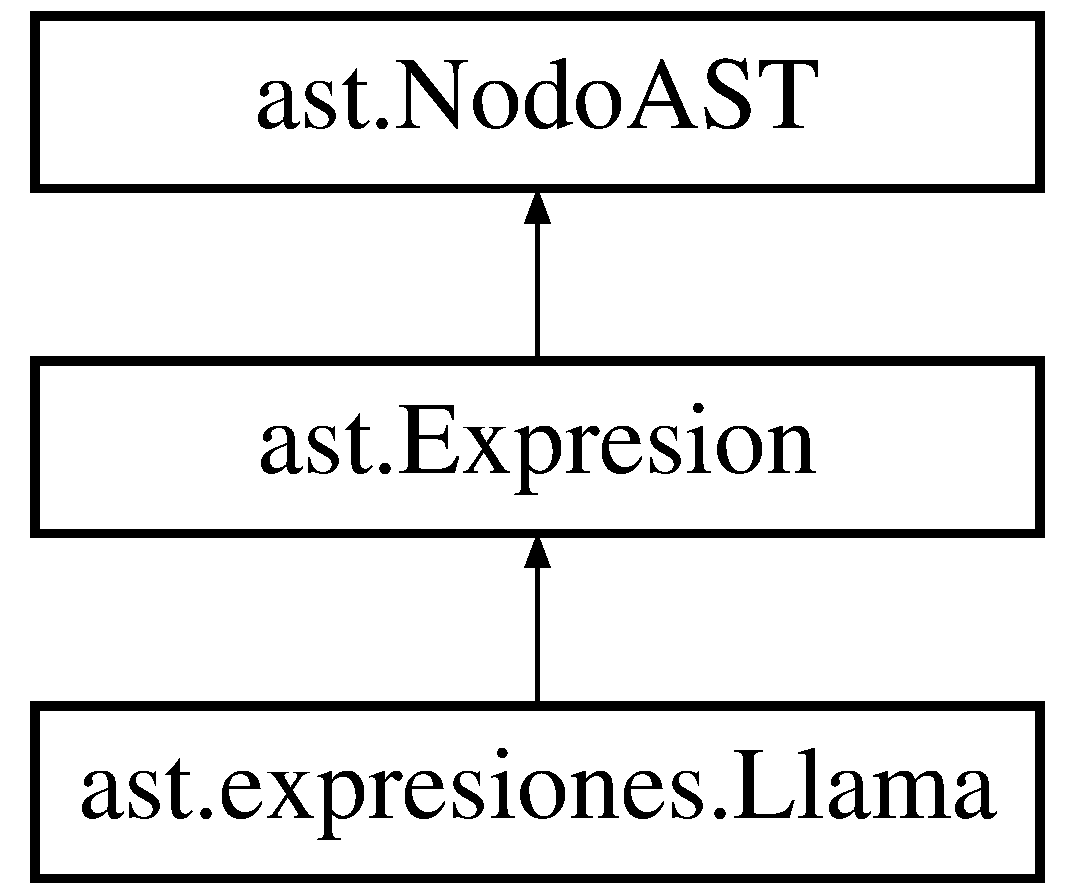
\includegraphics[height=3.000000cm]{classast_1_1expresiones_1_1_llama}
\end{center}
\end{figure}
\subsection*{Public Member Functions}
\begin{DoxyCompactItemize}
\item 
\mbox{\Hypertarget{classast_1_1expresiones_1_1_llama_a13ba50844e13b1aeb20c80a13b8412ec}\label{classast_1_1expresiones_1_1_llama_a13ba50844e13b1aeb20c80a13b8412ec}} 
{\bfseries Llama} (String id, Linked\+List$<$ \mbox{\hyperlink{interfaceast_1_1_nodo_a_s_t}{Nodo\+A\+ST}} $>$ valores, int linea, int col)
\item 
\mbox{\Hypertarget{classast_1_1expresiones_1_1_llama_a270a9d03242a447da6fa77ff1da3ed5c}\label{classast_1_1expresiones_1_1_llama_a270a9d03242a447da6fa77ff1da3ed5c}} 
{\bfseries Llama} (String id, int linea, int col)
\item 
\mbox{\Hypertarget{classast_1_1expresiones_1_1_llama_a09a04149a1401bdbf56144c98f4155f9}\label{classast_1_1expresiones_1_1_llama_a09a04149a1401bdbf56144c98f4155f9}} 
\mbox{\hyperlink{classentorno_1_1_tipo}{Tipo}} {\bfseries get\+Tipo} (\mbox{\hyperlink{classentorno_1_1_entorno}{Entorno}} ent)
\item 
\mbox{\Hypertarget{classast_1_1expresiones_1_1_llama_afb1af91740ba7d388e8f237fb59755a3}\label{classast_1_1expresiones_1_1_llama_afb1af91740ba7d388e8f237fb59755a3}} 
Object {\bfseries get\+Valor\+Implicito} (\mbox{\hyperlink{classentorno_1_1_entorno}{Entorno}} ent)
\item 
\mbox{\Hypertarget{classast_1_1expresiones_1_1_llama_a162c95ba7e816fea2647a74f3618e078}\label{classast_1_1expresiones_1_1_llama_a162c95ba7e816fea2647a74f3618e078}} 
int {\bfseries linea} ()
\item 
\mbox{\Hypertarget{classast_1_1expresiones_1_1_llama_ae4f9147f5e7874c0824d42de21975d34}\label{classast_1_1expresiones_1_1_llama_ae4f9147f5e7874c0824d42de21975d34}} 
int {\bfseries columna} ()
\item 
\mbox{\Hypertarget{classast_1_1expresiones_1_1_llama_afc370988a8403a8dd90436bdf640e75b}\label{classast_1_1expresiones_1_1_llama_afc370988a8403a8dd90436bdf640e75b}} 
String {\bfseries get\+Nombre} (String\+Builder builder, String parent, int cont)
\end{DoxyCompactItemize}


\subsection{Detailed Description}
\begin{DoxyAuthor}{Author}
p\+\_\+ab1 
\end{DoxyAuthor}


The documentation for this class was generated from the following file\+:\begin{DoxyCompactItemize}
\item 
src/ast/expresiones/Llama.\+java\end{DoxyCompactItemize}

\hypertarget{classast_1_1expresiones_1_1operaciones_1_1_logica}{}\section{ast.\+expresiones.\+operaciones.\+Logica Class Reference}
\label{classast_1_1expresiones_1_1operaciones_1_1_logica}\index{ast.\+expresiones.\+operaciones.\+Logica@{ast.\+expresiones.\+operaciones.\+Logica}}
Inheritance diagram for ast.\+expresiones.\+operaciones.\+Logica\+:\begin{figure}[H]
\begin{center}
\leavevmode
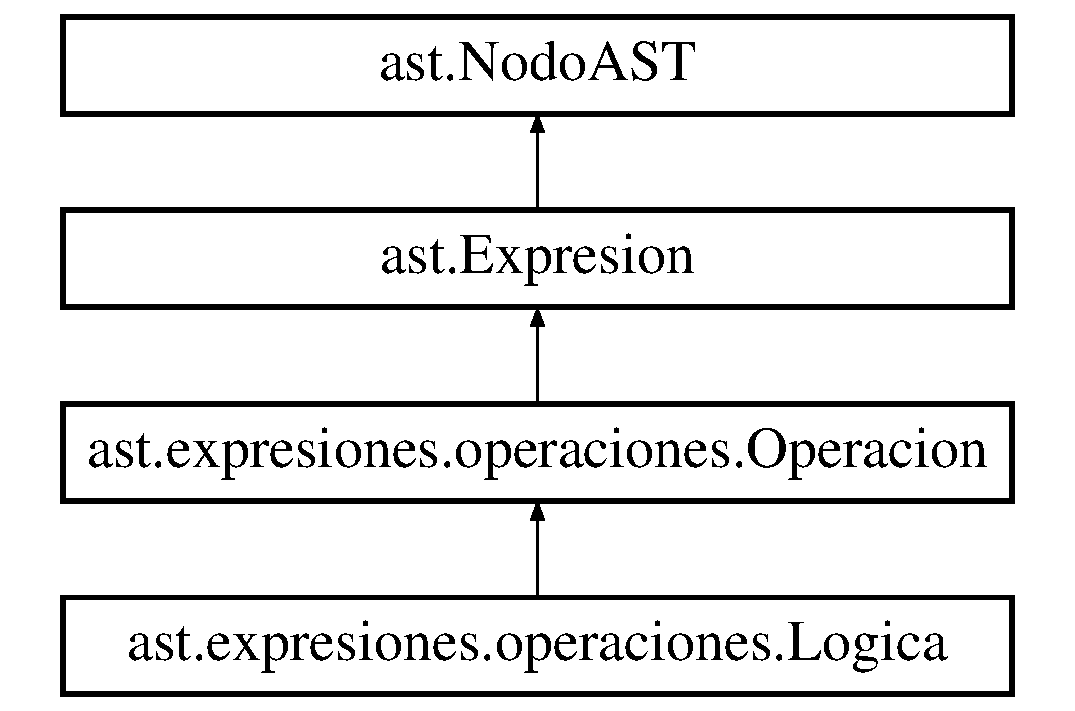
\includegraphics[height=4.000000cm]{classast_1_1expresiones_1_1operaciones_1_1_logica}
\end{center}
\end{figure}
\subsection*{Public Member Functions}
\begin{DoxyCompactItemize}
\item 
\mbox{\Hypertarget{classast_1_1expresiones_1_1operaciones_1_1_logica_af541241d78a1c5797c0538c4d42da81a}\label{classast_1_1expresiones_1_1operaciones_1_1_logica_af541241d78a1c5797c0538c4d42da81a}} 
{\bfseries Logica} (\mbox{\hyperlink{interfaceast_1_1_expresion}{Expresion}} op1, \mbox{\hyperlink{interfaceast_1_1_expresion}{Expresion}} op2, \mbox{\hyperlink{enumast_1_1expresiones_1_1operaciones_1_1_operacion_1_1_operador}{Operador}} operador, int col, int linea)
\item 
\mbox{\Hypertarget{classast_1_1expresiones_1_1operaciones_1_1_logica_a85f9a27373244ec27657c05a1de7b043}\label{classast_1_1expresiones_1_1operaciones_1_1_logica_a85f9a27373244ec27657c05a1de7b043}} 
{\bfseries Logica} (\mbox{\hyperlink{interfaceast_1_1_expresion}{Expresion}} opU, \mbox{\hyperlink{enumast_1_1expresiones_1_1operaciones_1_1_operacion_1_1_operador}{Operador}} operador, int col, int linea)
\item 
\mbox{\Hypertarget{classast_1_1expresiones_1_1operaciones_1_1_logica_a223bc43c5881a8a4bcad4ea7dc5c025e}\label{classast_1_1expresiones_1_1operaciones_1_1_logica_a223bc43c5881a8a4bcad4ea7dc5c025e}} 
\mbox{\hyperlink{classentorno_1_1_tipo}{Tipo}} {\bfseries tipo\+Dominante} (\mbox{\hyperlink{classentorno_1_1_tipo}{Tipo}} t1, \mbox{\hyperlink{classentorno_1_1_tipo}{Tipo}} t2)
\item 
\mbox{\Hypertarget{classast_1_1expresiones_1_1operaciones_1_1_logica_afcfaee492292e2e8b96145f65e4b383e}\label{classast_1_1expresiones_1_1operaciones_1_1_logica_afcfaee492292e2e8b96145f65e4b383e}} 
\mbox{\hyperlink{classentorno_1_1_tipo}{Tipo}} {\bfseries get\+Tipo} (\mbox{\hyperlink{classentorno_1_1_entorno}{Entorno}} ent)
\item 
\mbox{\Hypertarget{classast_1_1expresiones_1_1operaciones_1_1_logica_aa945bbbec453832fbf34f6a27ea6cc63}\label{classast_1_1expresiones_1_1operaciones_1_1_logica_aa945bbbec453832fbf34f6a27ea6cc63}} 
Object {\bfseries get\+Valor\+Implicito} (\mbox{\hyperlink{classentorno_1_1_entorno}{Entorno}} ent)
\item 
\mbox{\Hypertarget{classast_1_1expresiones_1_1operaciones_1_1_logica_a94e434f3871c114bb1191fcbb182b77f}\label{classast_1_1expresiones_1_1operaciones_1_1_logica_a94e434f3871c114bb1191fcbb182b77f}} 
String {\bfseries get\+Nombre} (String\+Builder builder, String parent, int cont)
\end{DoxyCompactItemize}


\subsection{Detailed Description}
\begin{DoxyAuthor}{Author}
p\+\_\+ab1 
\end{DoxyAuthor}


The documentation for this class was generated from the following file\+:\begin{DoxyCompactItemize}
\item 
src/ast/expresiones/operaciones/Logica.\+java\end{DoxyCompactItemize}

\hypertarget{class_j_lex_1_1_main}{}\section{J\+Lex.\+Main Class Reference}
\label{class_j_lex_1_1_main}\index{J\+Lex.\+Main@{J\+Lex.\+Main}}
\subsection*{Static Public Member Functions}
\begin{DoxyCompactItemize}
\item 
\mbox{\Hypertarget{class_j_lex_1_1_main_ad93dc43626ab1d1450cc9df0db2f12c9}\label{class_j_lex_1_1_main_ad93dc43626ab1d1450cc9df0db2f12c9}} 
static void {\bfseries main} (String arg\mbox{[}$\,$\mbox{]})  throws java.\+io.\+I\+O\+Exception       
\end{DoxyCompactItemize}


The documentation for this class was generated from the following file\+:\begin{DoxyCompactItemize}
\item 
src/analizadores/\+J\+Lex/Main.\+java\end{DoxyCompactItemize}

\hypertarget{classast_1_1instrucciones_1_1funciones_1_1_modificador_matrix}{}\section{ast.\+instrucciones.\+funciones.\+Modificador\+Matrix Class Reference}
\label{classast_1_1instrucciones_1_1funciones_1_1_modificador_matrix}\index{ast.\+instrucciones.\+funciones.\+Modificador\+Matrix@{ast.\+instrucciones.\+funciones.\+Modificador\+Matrix}}
\subsection*{Public Member Functions}
\begin{DoxyCompactItemize}
\item 
\mbox{\Hypertarget{classast_1_1instrucciones_1_1funciones_1_1_modificador_matrix_a9254b3058a70f02e868c56ae9afaa2ae}\label{classast_1_1instrucciones_1_1funciones_1_1_modificador_matrix_a9254b3058a70f02e868c56ae9afaa2ae}} 
{\bfseries Modificador\+Matrix} (\mbox{\hyperlink{classentorno_1_1nodo_exp}{nodo\+Exp}} e, Object\mbox{[}$\,$\mbox{]}\mbox{[}$\,$\mbox{]} mat, \mbox{\hyperlink{classentorno_1_1_entorno}{Entorno}} ent, \mbox{\hyperlink{classentorno_1_1_simbolo}{Simbolo}} sim)
\item 
\mbox{\Hypertarget{classast_1_1instrucciones_1_1funciones_1_1_modificador_matrix_ab702e68a1067bedaa1c698c84f4ecbb9}\label{classast_1_1instrucciones_1_1funciones_1_1_modificador_matrix_ab702e68a1067bedaa1c698c84f4ecbb9}} 
void {\bfseries cambiar\+Valor} (Object valor\+Nuevo)
\end{DoxyCompactItemize}


\subsection{Detailed Description}
\begin{DoxyAuthor}{Author}
hp 
\end{DoxyAuthor}


The documentation for this class was generated from the following file\+:\begin{DoxyCompactItemize}
\item 
src/ast/instrucciones/funciones/Modificador\+Matrix.\+java\end{DoxyCompactItemize}

\hypertarget{classast_1_1instrucciones_1_1funciones_1_1n_matrix}{}\section{ast.\+instrucciones.\+funciones.\+n\+Matrix Class Reference}
\label{classast_1_1instrucciones_1_1funciones_1_1n_matrix}\index{ast.\+instrucciones.\+funciones.\+n\+Matrix@{ast.\+instrucciones.\+funciones.\+n\+Matrix}}
Inheritance diagram for ast.\+instrucciones.\+funciones.\+n\+Matrix\+:\begin{figure}[H]
\begin{center}
\leavevmode
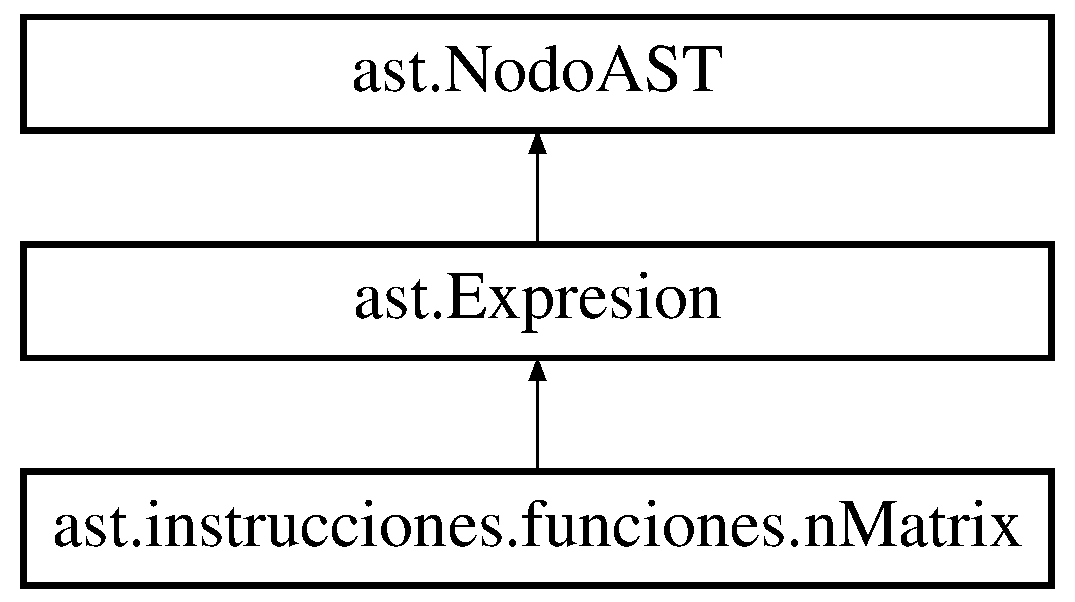
\includegraphics[height=3.000000cm]{classast_1_1instrucciones_1_1funciones_1_1n_matrix}
\end{center}
\end{figure}
\subsection*{Public Member Functions}
\begin{DoxyCompactItemize}
\item 
\mbox{\Hypertarget{classast_1_1instrucciones_1_1funciones_1_1n_matrix_a45a255f176702d226a85f0159219883f}\label{classast_1_1instrucciones_1_1funciones_1_1n_matrix_a45a255f176702d226a85f0159219883f}} 
{\bfseries n\+Matrix} (String id, Linked\+List$<$ \mbox{\hyperlink{interfaceast_1_1_nodo_a_s_t}{Nodo\+A\+ST}} $>$ valor, int linea, int col)
\item 
\mbox{\Hypertarget{classast_1_1instrucciones_1_1funciones_1_1n_matrix_a6ff5c31931e30db663e0a5d9202c8eca}\label{classast_1_1instrucciones_1_1funciones_1_1n_matrix_a6ff5c31931e30db663e0a5d9202c8eca}} 
\mbox{\hyperlink{classentorno_1_1_tipo}{Tipo}} {\bfseries get\+Tipo} (\mbox{\hyperlink{classentorno_1_1_entorno}{Entorno}} ent)
\item 
\mbox{\Hypertarget{classast_1_1instrucciones_1_1funciones_1_1n_matrix_a080b12aa8b0269e80f6d998f082ff50f}\label{classast_1_1instrucciones_1_1funciones_1_1n_matrix_a080b12aa8b0269e80f6d998f082ff50f}} 
Object {\bfseries get\+Valor\+Implicito} (\mbox{\hyperlink{classentorno_1_1_entorno}{Entorno}} ent)
\item 
\mbox{\Hypertarget{classast_1_1instrucciones_1_1funciones_1_1n_matrix_afd37b860aef9e8320b956b9a22d854a7}\label{classast_1_1instrucciones_1_1funciones_1_1n_matrix_afd37b860aef9e8320b956b9a22d854a7}} 
int {\bfseries linea} ()
\item 
\mbox{\Hypertarget{classast_1_1instrucciones_1_1funciones_1_1n_matrix_ab0320d0e05a73f73b4371621817d120d}\label{classast_1_1instrucciones_1_1funciones_1_1n_matrix_ab0320d0e05a73f73b4371621817d120d}} 
int {\bfseries columna} ()
\item 
\mbox{\Hypertarget{classast_1_1instrucciones_1_1funciones_1_1n_matrix_ad972429964b6bc38948d970674001f39}\label{classast_1_1instrucciones_1_1funciones_1_1n_matrix_ad972429964b6bc38948d970674001f39}} 
String {\bfseries get\+Nombre} (String\+Builder builder, String parent, int cont)
\end{DoxyCompactItemize}


\subsection{Detailed Description}
\begin{DoxyAuthor}{Author}
p\+\_\+ab1 
\end{DoxyAuthor}


The documentation for this class was generated from the following file\+:\begin{DoxyCompactItemize}
\item 
src/ast/instrucciones/funciones/n\+Matrix.\+java\end{DoxyCompactItemize}

\hypertarget{interfaceast_1_1_nodo_a_s_t}{}\section{ast.\+Nodo\+A\+ST Interface Reference}
\label{interfaceast_1_1_nodo_a_s_t}\index{ast.\+Nodo\+A\+ST@{ast.\+Nodo\+A\+ST}}
Inheritance diagram for ast.\+Nodo\+A\+ST\+:\begin{figure}[H]
\begin{center}
\leavevmode
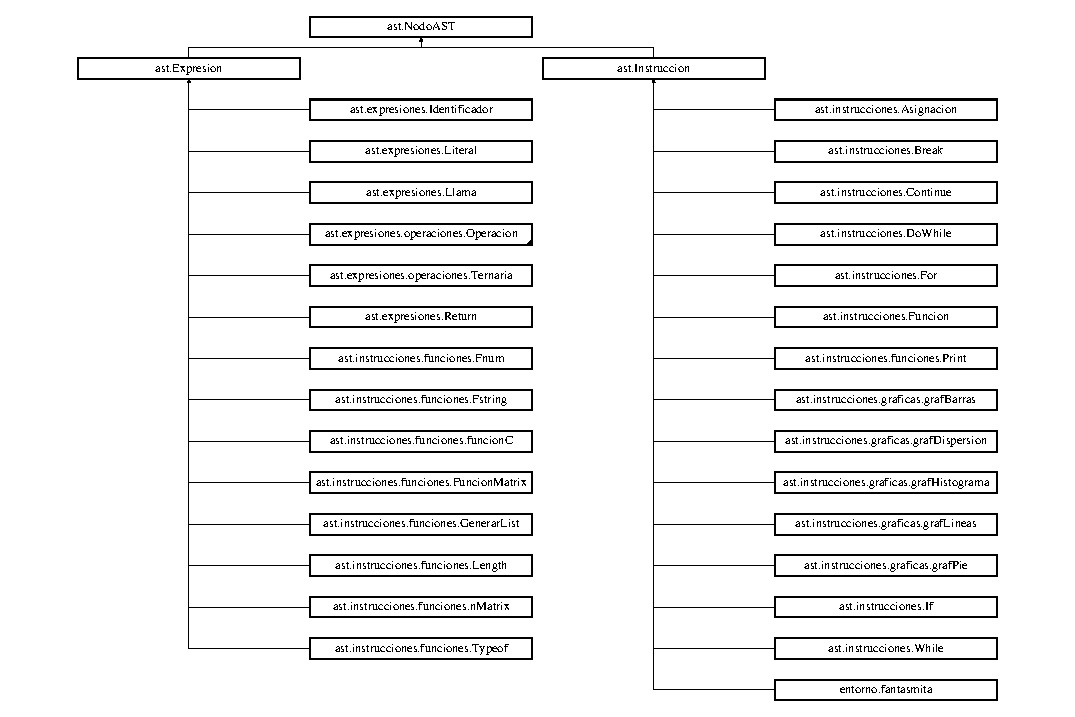
\includegraphics[height=9.189190cm]{interfaceast_1_1_nodo_a_s_t}
\end{center}
\end{figure}
\subsection*{Public Member Functions}
\begin{DoxyCompactItemize}
\item 
\mbox{\Hypertarget{interfaceast_1_1_nodo_a_s_t_a16221a6d574a196e07ac3ae6a4364456}\label{interfaceast_1_1_nodo_a_s_t_a16221a6d574a196e07ac3ae6a4364456}} 
int {\bfseries linea} ()
\item 
\mbox{\Hypertarget{interfaceast_1_1_nodo_a_s_t_a524e3c279ffcf90d1192645780e606bc}\label{interfaceast_1_1_nodo_a_s_t_a524e3c279ffcf90d1192645780e606bc}} 
int {\bfseries columna} ()
\item 
\mbox{\Hypertarget{interfaceast_1_1_nodo_a_s_t_a13a69d91a32b969576752c1da53d103f}\label{interfaceast_1_1_nodo_a_s_t_a13a69d91a32b969576752c1da53d103f}} 
String {\bfseries get\+Nombre} (String\+Builder builder, String parent, int cont)
\end{DoxyCompactItemize}


\subsection{Detailed Description}
\begin{DoxyAuthor}{Author}
p\+\_\+ab1 
\end{DoxyAuthor}


The documentation for this interface was generated from the following file\+:\begin{DoxyCompactItemize}
\item 
src/ast/Nodo\+A\+S\+T.\+java\end{DoxyCompactItemize}

\hypertarget{classentorno_1_1nodo_exp}{}\section{entorno.\+nodo\+Exp Class Reference}
\label{classentorno_1_1nodo_exp}\index{entorno.\+nodo\+Exp@{entorno.\+nodo\+Exp}}
\subsection*{Public Member Functions}
\begin{DoxyCompactItemize}
\item 
\mbox{\Hypertarget{classentorno_1_1nodo_exp_a6f62612e1371b6b7b136d0300873dd2f}\label{classentorno_1_1nodo_exp_a6f62612e1371b6b7b136d0300873dd2f}} 
{\bfseries nodo\+Exp} (\mbox{\hyperlink{interfaceast_1_1_expresion}{Expresion}} exp1, Simbolo.\+Acc tipo\+Acceso)
\item 
\mbox{\Hypertarget{classentorno_1_1nodo_exp_ac107d179f4dad7e0b4c502efb8658323}\label{classentorno_1_1nodo_exp_ac107d179f4dad7e0b4c502efb8658323}} 
{\bfseries nodo\+Exp} (\mbox{\hyperlink{interfaceast_1_1_expresion}{Expresion}} exp1, \mbox{\hyperlink{interfaceast_1_1_expresion}{Expresion}} exp2, Simbolo.\+Acc tipo\+Acceso)
\item 
\mbox{\Hypertarget{classentorno_1_1nodo_exp_ac4b421f105548c387ef018a71d81d758}\label{classentorno_1_1nodo_exp_ac4b421f105548c387ef018a71d81d758}} 
\mbox{\hyperlink{interfaceast_1_1_expresion}{Expresion}} {\bfseries get\+Exp1} ()
\item 
\mbox{\Hypertarget{classentorno_1_1nodo_exp_adfc2c33135565d52e8f61d409170fa08}\label{classentorno_1_1nodo_exp_adfc2c33135565d52e8f61d409170fa08}} 
void {\bfseries set\+Exp1} (\mbox{\hyperlink{interfaceast_1_1_expresion}{Expresion}} exp)
\item 
\mbox{\Hypertarget{classentorno_1_1nodo_exp_a5015c3c9f7a4c57d2e8555f6096f4eb1}\label{classentorno_1_1nodo_exp_a5015c3c9f7a4c57d2e8555f6096f4eb1}} 
Simbolo.\+Acc {\bfseries get\+Tipo\+Acceso} ()
\item 
\mbox{\Hypertarget{classentorno_1_1nodo_exp_a2a472637b568f62b4fe5a7d77fae0cab}\label{classentorno_1_1nodo_exp_a2a472637b568f62b4fe5a7d77fae0cab}} 
void {\bfseries set\+Tipo\+Acceso} (Simbolo.\+Acc tipo\+Acceso)
\item 
\mbox{\Hypertarget{classentorno_1_1nodo_exp_a0ef0e42cf7b4c354cf5718b1df9a23ec}\label{classentorno_1_1nodo_exp_a0ef0e42cf7b4c354cf5718b1df9a23ec}} 
\mbox{\hyperlink{interfaceast_1_1_expresion}{Expresion}} {\bfseries get\+Exp2} ()
\item 
\mbox{\Hypertarget{classentorno_1_1nodo_exp_a9dbde43689ca543ca79432ad096f503a}\label{classentorno_1_1nodo_exp_a9dbde43689ca543ca79432ad096f503a}} 
void {\bfseries set\+Exp2} (\mbox{\hyperlink{interfaceast_1_1_expresion}{Expresion}} exp2)
\end{DoxyCompactItemize}


\subsection{Detailed Description}
\begin{DoxyAuthor}{Author}
p\+\_\+ab1 
\end{DoxyAuthor}


The documentation for this class was generated from the following file\+:\begin{DoxyCompactItemize}
\item 
src/entorno/nodo\+Exp.\+java\end{DoxyCompactItemize}

\hypertarget{classolc2_1_1p1__201504242_1_1_o_l_c2_p1__201504242}{}\section{olc2.\+p1\+\_\+201504242.\+O\+L\+C2\+P1\+\_\+201504242 Class Reference}
\label{classolc2_1_1p1__201504242_1_1_o_l_c2_p1__201504242}\index{olc2.\+p1\+\_\+201504242.\+O\+L\+C2\+P1\+\_\+201504242@{olc2.\+p1\+\_\+201504242.\+O\+L\+C2\+P1\+\_\+201504242}}
\subsection*{Static Public Member Functions}
\begin{DoxyCompactItemize}
\item 
static void \mbox{\hyperlink{classolc2_1_1p1__201504242_1_1_o_l_c2_p1__201504242_a5bf79504e3877c2dc8715e2e690b9653}{main}} (String\mbox{[}$\,$\mbox{]} args)
\end{DoxyCompactItemize}
\subsection*{Static Public Attributes}
\begin{DoxyCompactItemize}
\item 
\mbox{\Hypertarget{classolc2_1_1p1__201504242_1_1_o_l_c2_p1__201504242_a21bf22cd1c336781d9102e71dc31be9b}\label{classolc2_1_1p1__201504242_1_1_o_l_c2_p1__201504242_a21bf22cd1c336781d9102e71dc31be9b}} 
static \mbox{\hyperlink{classolc2_1_1p1__201504242_1_1_ventana}{Ventana}} {\bfseries ven}
\end{DoxyCompactItemize}


\subsection{Detailed Description}
\begin{DoxyAuthor}{Author}
p\+\_\+ab1 
\end{DoxyAuthor}


\subsection{Member Function Documentation}
\mbox{\Hypertarget{classolc2_1_1p1__201504242_1_1_o_l_c2_p1__201504242_a5bf79504e3877c2dc8715e2e690b9653}\label{classolc2_1_1p1__201504242_1_1_o_l_c2_p1__201504242_a5bf79504e3877c2dc8715e2e690b9653}} 
\index{olc2\+::p1\+\_\+201504242\+::\+O\+L\+C2\+P1\+\_\+201504242@{olc2\+::p1\+\_\+201504242\+::\+O\+L\+C2\+P1\+\_\+201504242}!main@{main}}
\index{main@{main}!olc2\+::p1\+\_\+201504242\+::\+O\+L\+C2\+P1\+\_\+201504242@{olc2\+::p1\+\_\+201504242\+::\+O\+L\+C2\+P1\+\_\+201504242}}
\subsubsection{\texorpdfstring{main()}{main()}}
{\footnotesize\ttfamily static void olc2.\+p1\+\_\+201504242.\+O\+L\+C2\+P1\+\_\+201504242.\+main (\begin{DoxyParamCaption}\item[{String \mbox{[}$\,$\mbox{]}}]{args }\end{DoxyParamCaption})\hspace{0.3cm}{\ttfamily [static]}}


\begin{DoxyParams}{Parameters}
{\em args} & the command line arguments \\
\hline
\end{DoxyParams}


The documentation for this class was generated from the following file\+:\begin{DoxyCompactItemize}
\item 
src/olc2/p1\+\_\+201504242/O\+L\+C2\+P1\+\_\+201504242.\+java\end{DoxyCompactItemize}

\hypertarget{classast_1_1expresiones_1_1operaciones_1_1_operacion}{}\section{ast.\+expresiones.\+operaciones.\+Operacion Class Reference}
\label{classast_1_1expresiones_1_1operaciones_1_1_operacion}\index{ast.\+expresiones.\+operaciones.\+Operacion@{ast.\+expresiones.\+operaciones.\+Operacion}}
Inheritance diagram for ast.\+expresiones.\+operaciones.\+Operacion\+:\begin{figure}[H]
\begin{center}
\leavevmode
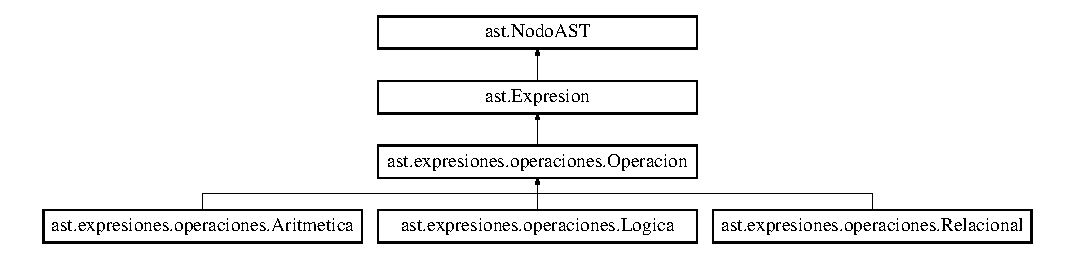
\includegraphics[height=3.035230cm]{classast_1_1expresiones_1_1operaciones_1_1_operacion}
\end{center}
\end{figure}
\subsection*{Classes}
\begin{DoxyCompactItemize}
\item 
enum \mbox{\hyperlink{enumast_1_1expresiones_1_1operaciones_1_1_operacion_1_1_operador}{Operador}}
\end{DoxyCompactItemize}
\subsection*{Public Member Functions}
\begin{DoxyCompactItemize}
\item 
\mbox{\Hypertarget{classast_1_1expresiones_1_1operaciones_1_1_operacion_a9ba85d4f6d374c3bc903507e795da4b3}\label{classast_1_1expresiones_1_1operaciones_1_1_operacion_a9ba85d4f6d374c3bc903507e795da4b3}} 
{\bfseries Operacion} (\mbox{\hyperlink{interfaceast_1_1_expresion}{Expresion}} op1, \mbox{\hyperlink{interfaceast_1_1_expresion}{Expresion}} op2, \mbox{\hyperlink{enumast_1_1expresiones_1_1operaciones_1_1_operacion_1_1_operador}{Operador}} operador, int col, int fila)
\item 
\mbox{\Hypertarget{classast_1_1expresiones_1_1operaciones_1_1_operacion_a7b684f5095981b6fa965e77262a5aacd}\label{classast_1_1expresiones_1_1operaciones_1_1_operacion_a7b684f5095981b6fa965e77262a5aacd}} 
{\bfseries Operacion} (\mbox{\hyperlink{interfaceast_1_1_expresion}{Expresion}} opU, \mbox{\hyperlink{enumast_1_1expresiones_1_1operaciones_1_1_operacion_1_1_operador}{Operador}} operador, int col, int fila)
\item 
\mbox{\Hypertarget{classast_1_1expresiones_1_1operaciones_1_1_operacion_aa445579ac0c73cfbfb07b9d27e59c059}\label{classast_1_1expresiones_1_1operaciones_1_1_operacion_aa445579ac0c73cfbfb07b9d27e59c059}} 
abstract \mbox{\hyperlink{classentorno_1_1_tipo}{Tipo}} {\bfseries tipo\+Dominante} (\mbox{\hyperlink{classentorno_1_1_tipo}{Tipo}} t1, \mbox{\hyperlink{classentorno_1_1_tipo}{Tipo}} t2)
\item 
\mbox{\Hypertarget{classast_1_1expresiones_1_1operaciones_1_1_operacion_a0e6c9445b5becf5a531128563b3ef77e}\label{classast_1_1expresiones_1_1operaciones_1_1_operacion_a0e6c9445b5becf5a531128563b3ef77e}} 
int {\bfseries linea} ()
\item 
\mbox{\Hypertarget{classast_1_1expresiones_1_1operaciones_1_1_operacion_a5920863beab978a6122303148b3b3b8f}\label{classast_1_1expresiones_1_1operaciones_1_1_operacion_a5920863beab978a6122303148b3b3b8f}} 
int {\bfseries columna} ()
\end{DoxyCompactItemize}


\subsection{Detailed Description}
\begin{DoxyAuthor}{Author}
p\+\_\+ab1 
\end{DoxyAuthor}


The documentation for this class was generated from the following file\+:\begin{DoxyCompactItemize}
\item 
src/ast/expresiones/operaciones/Operacion.\+java\end{DoxyCompactItemize}

\hypertarget{enumast_1_1expresiones_1_1operaciones_1_1_operacion_1_1_operador}{}\section{ast.\+expresiones.\+operaciones.\+Operacion.\+Operador Enum Reference}
\label{enumast_1_1expresiones_1_1operaciones_1_1_operacion_1_1_operador}\index{ast.\+expresiones.\+operaciones.\+Operacion.\+Operador@{ast.\+expresiones.\+operaciones.\+Operacion.\+Operador}}
\subsection*{Public Attributes}
\begin{DoxyCompactItemize}
\item 
\mbox{\Hypertarget{enumast_1_1expresiones_1_1operaciones_1_1_operacion_1_1_operador_a2f6c295493f152893cd6009017110a18}\label{enumast_1_1expresiones_1_1operaciones_1_1_operacion_1_1_operador_a2f6c295493f152893cd6009017110a18}} 
{\bfseries S\+U\+MA}
\item 
\mbox{\Hypertarget{enumast_1_1expresiones_1_1operaciones_1_1_operacion_1_1_operador_aa8fb89f748f5535fb1eec42e724c908c}\label{enumast_1_1expresiones_1_1operaciones_1_1_operacion_1_1_operador_aa8fb89f748f5535fb1eec42e724c908c}} 
{\bfseries R\+E\+S\+TA}
\item 
\mbox{\Hypertarget{enumast_1_1expresiones_1_1operaciones_1_1_operacion_1_1_operador_ac57dd8e6cf8358967b941a2ce9e7cfbb}\label{enumast_1_1expresiones_1_1operaciones_1_1_operacion_1_1_operador_ac57dd8e6cf8358967b941a2ce9e7cfbb}} 
{\bfseries M\+U\+L\+T\+I\+P\+L\+I\+C\+A\+C\+I\+ON}
\item 
\mbox{\Hypertarget{enumast_1_1expresiones_1_1operaciones_1_1_operacion_1_1_operador_a538e73edc9f70ea1839545019b5013cf}\label{enumast_1_1expresiones_1_1operaciones_1_1_operacion_1_1_operador_a538e73edc9f70ea1839545019b5013cf}} 
{\bfseries D\+I\+V\+I\+S\+I\+ON}
\item 
\mbox{\Hypertarget{enumast_1_1expresiones_1_1operaciones_1_1_operacion_1_1_operador_a82b4784bf5fb9d975b5060da1f8d707c}\label{enumast_1_1expresiones_1_1operaciones_1_1_operacion_1_1_operador_a82b4784bf5fb9d975b5060da1f8d707c}} 
{\bfseries P\+O\+T\+E\+N\+C\+IA}
\item 
\mbox{\Hypertarget{enumast_1_1expresiones_1_1operaciones_1_1_operacion_1_1_operador_a0cd75ca7f411e1311fc7c30c7b8310f5}\label{enumast_1_1expresiones_1_1operaciones_1_1_operacion_1_1_operador_a0cd75ca7f411e1311fc7c30c7b8310f5}} 
{\bfseries M\+O\+D\+U\+LO}
\item 
\mbox{\Hypertarget{enumast_1_1expresiones_1_1operaciones_1_1_operacion_1_1_operador_a5952580b302ac0c254a0d6f7fc03bb99}\label{enumast_1_1expresiones_1_1operaciones_1_1_operacion_1_1_operador_a5952580b302ac0c254a0d6f7fc03bb99}} 
{\bfseries M\+E\+N\+O\+S\+\_\+\+U\+N\+A\+R\+IO}
\item 
\mbox{\Hypertarget{enumast_1_1expresiones_1_1operaciones_1_1_operacion_1_1_operador_abcdca12e3fe682583e0a54d02b65894e}\label{enumast_1_1expresiones_1_1operaciones_1_1_operacion_1_1_operador_abcdca12e3fe682583e0a54d02b65894e}} 
{\bfseries M\+A\+Y\+O\+R\+\_\+\+Q\+UE}
\item 
\mbox{\Hypertarget{enumast_1_1expresiones_1_1operaciones_1_1_operacion_1_1_operador_a47c84206ecd807509229809243d9f8e6}\label{enumast_1_1expresiones_1_1operaciones_1_1_operacion_1_1_operador_a47c84206ecd807509229809243d9f8e6}} 
{\bfseries M\+A\+Y\+O\+R\+\_\+\+I\+G\+U\+AL}
\item 
\mbox{\Hypertarget{enumast_1_1expresiones_1_1operaciones_1_1_operacion_1_1_operador_a11be6b6dcce6203e1363791af6f1eadc}\label{enumast_1_1expresiones_1_1operaciones_1_1_operacion_1_1_operador_a11be6b6dcce6203e1363791af6f1eadc}} 
{\bfseries M\+E\+N\+O\+R\+\_\+\+Q\+UE}
\item 
\mbox{\Hypertarget{enumast_1_1expresiones_1_1operaciones_1_1_operacion_1_1_operador_aa97a1945717d1999c0b1b8d32bf00167}\label{enumast_1_1expresiones_1_1operaciones_1_1_operacion_1_1_operador_aa97a1945717d1999c0b1b8d32bf00167}} 
{\bfseries M\+E\+N\+O\+R\+\_\+\+I\+G\+U\+AL}
\item 
\mbox{\Hypertarget{enumast_1_1expresiones_1_1operaciones_1_1_operacion_1_1_operador_a5581edb895d626fc5ee1e692caafc87c}\label{enumast_1_1expresiones_1_1operaciones_1_1_operacion_1_1_operador_a5581edb895d626fc5ee1e692caafc87c}} 
{\bfseries I\+G\+U\+A\+L\+\_\+\+I\+G\+U\+AL}
\item 
\mbox{\Hypertarget{enumast_1_1expresiones_1_1operaciones_1_1_operacion_1_1_operador_a027b456cac1444dfe829a97e5f150399}\label{enumast_1_1expresiones_1_1operaciones_1_1_operacion_1_1_operador_a027b456cac1444dfe829a97e5f150399}} 
{\bfseries D\+I\+F\+E\+R\+E\+N\+T\+E\+\_\+\+Q\+UE}
\item 
\mbox{\Hypertarget{enumast_1_1expresiones_1_1operaciones_1_1_operacion_1_1_operador_a62da7a279a6c23343527034e5131e8d9}\label{enumast_1_1expresiones_1_1operaciones_1_1_operacion_1_1_operador_a62da7a279a6c23343527034e5131e8d9}} 
{\bfseries OR}
\item 
\mbox{\Hypertarget{enumast_1_1expresiones_1_1operaciones_1_1_operacion_1_1_operador_aafca71c0d0676b9f21f229939dc526fa}\label{enumast_1_1expresiones_1_1operaciones_1_1_operacion_1_1_operador_aafca71c0d0676b9f21f229939dc526fa}} 
{\bfseries X\+OR}
\item 
\mbox{\Hypertarget{enumast_1_1expresiones_1_1operaciones_1_1_operacion_1_1_operador_a7ddaa57c5b65acc4c96b97b1bc202653}\label{enumast_1_1expresiones_1_1operaciones_1_1_operacion_1_1_operador_a7ddaa57c5b65acc4c96b97b1bc202653}} 
{\bfseries A\+ND}
\item 
\mbox{\Hypertarget{enumast_1_1expresiones_1_1operaciones_1_1_operacion_1_1_operador_a485481620052829dbedd6cacfd1ca560}\label{enumast_1_1expresiones_1_1operaciones_1_1_operacion_1_1_operador_a485481620052829dbedd6cacfd1ca560}} 
{\bfseries N\+OT}
\item 
\mbox{\Hypertarget{enumast_1_1expresiones_1_1operaciones_1_1_operacion_1_1_operador_a8cc87ba10520b3bc890b06ca3ccecd55}\label{enumast_1_1expresiones_1_1operaciones_1_1_operacion_1_1_operador_a8cc87ba10520b3bc890b06ca3ccecd55}} 
{\bfseries T\+E\+R\+N\+A\+R\+IA}
\item 
\mbox{\Hypertarget{enumast_1_1expresiones_1_1operaciones_1_1_operacion_1_1_operador_a2403ae17cfa347021d658cc975c08ca7}\label{enumast_1_1expresiones_1_1operaciones_1_1_operacion_1_1_operador_a2403ae17cfa347021d658cc975c08ca7}} 
{\bfseries D\+E\+S\+C\+O\+N\+O\+C\+I\+DO}
\end{DoxyCompactItemize}


The documentation for this enum was generated from the following file\+:\begin{DoxyCompactItemize}
\item 
src/ast/expresiones/operaciones/Operacion.\+java\end{DoxyCompactItemize}

\hypertarget{classanalizadores_1_1_parse_exception}{}\section{analizadores.\+Parse\+Exception Class Reference}
\label{classanalizadores_1_1_parse_exception}\index{analizadores.\+Parse\+Exception@{analizadores.\+Parse\+Exception}}
Inheritance diagram for analizadores.\+Parse\+Exception\+:\begin{figure}[H]
\begin{center}
\leavevmode
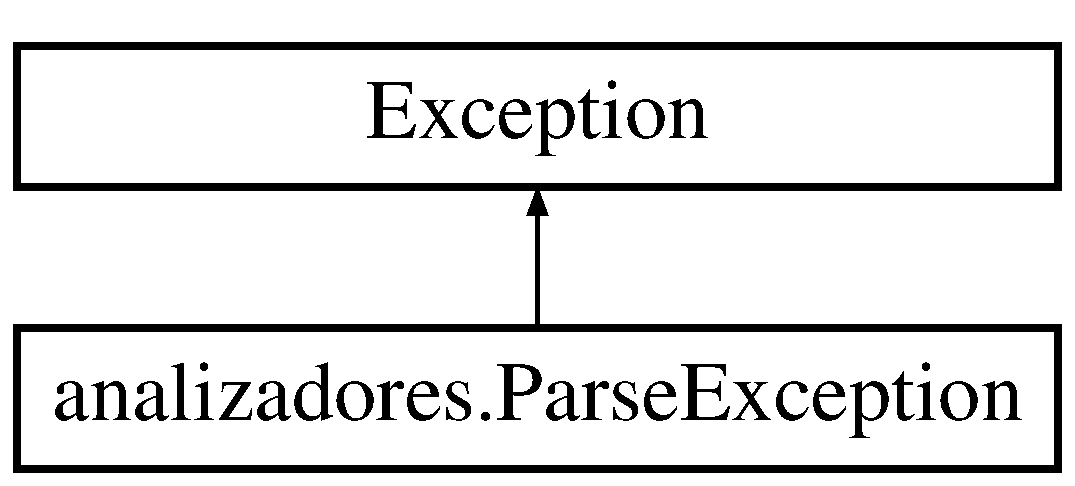
\includegraphics[height=2.000000cm]{classanalizadores_1_1_parse_exception}
\end{center}
\end{figure}
\subsection*{Public Member Functions}
\begin{DoxyCompactItemize}
\item 
\mbox{\hyperlink{classanalizadores_1_1_parse_exception_ac9289cbed3fc5347a25e1727070311e9}{Parse\+Exception}} (\mbox{\hyperlink{classanalizadores_1_1_token}{Token}} current\+Token\+Val, int\mbox{[}$\,$\mbox{]}\mbox{[}$\,$\mbox{]} expected\+Token\+Sequences\+Val, String\mbox{[}$\,$\mbox{]} token\+Image\+Val)
\item 
\mbox{\hyperlink{classanalizadores_1_1_parse_exception_ad2caa939d34e9a1a6f550e795468bac9}{Parse\+Exception}} ()
\item 
\mbox{\hyperlink{classanalizadores_1_1_parse_exception_ad521e60f04650096c71062ec8bf0c0a4}{Parse\+Exception}} (String message)
\item 
String \mbox{\hyperlink{classanalizadores_1_1_parse_exception_a6b54780b5e7d3ca5f905cef4a218eff6}{get\+Message}} ()
\end{DoxyCompactItemize}
\subsection*{Public Attributes}
\begin{DoxyCompactItemize}
\item 
\mbox{\hyperlink{classanalizadores_1_1_token}{Token}} \mbox{\hyperlink{classanalizadores_1_1_parse_exception_a5e7dae6899708a852cc7410e52d090f2}{current\+Token}}
\item 
int \mbox{[}$\,$\mbox{]}\mbox{[}$\,$\mbox{]} \mbox{\hyperlink{classanalizadores_1_1_parse_exception_aef57ab03c5f063e50c0eaa6b0e525946}{expected\+Token\+Sequences}}
\item 
String \mbox{[}$\,$\mbox{]} \mbox{\hyperlink{classanalizadores_1_1_parse_exception_a8d39ada57041e6c5b993d2b6fd66d6cc}{token\+Image}}
\end{DoxyCompactItemize}
\subsection*{Protected Member Functions}
\begin{DoxyCompactItemize}
\item 
String \mbox{\hyperlink{classanalizadores_1_1_parse_exception_ad9fe07877080d0a28daa4d139860d110}{add\+\_\+escapes}} (String str)
\end{DoxyCompactItemize}
\subsection*{Protected Attributes}
\begin{DoxyCompactItemize}
\item 
boolean \mbox{\hyperlink{classanalizadores_1_1_parse_exception_a24ccd87a4ef257c9e62418a4009bc5cd}{special\+Constructor}}
\item 
String \mbox{\hyperlink{classanalizadores_1_1_parse_exception_a6dceb2e8353ece2d7d2e2b86a8c7147d}{eol}} = System.\+get\+Property(\char`\"{}line.\+separator\char`\"{}, \char`\"{}\textbackslash{}n\char`\"{})
\end{DoxyCompactItemize}


\subsection{Detailed Description}
This exception is thrown when parse errors are encountered. You can explicitly create objects of this exception type by calling the method generate\+Parse\+Exception in the generated parser.

You can modify this class to customize your error reporting mechanisms so long as you retain the public fields. 

\subsection{Constructor \& Destructor Documentation}
\mbox{\Hypertarget{classanalizadores_1_1_parse_exception_ac9289cbed3fc5347a25e1727070311e9}\label{classanalizadores_1_1_parse_exception_ac9289cbed3fc5347a25e1727070311e9}} 
\index{analizadores\+::\+Parse\+Exception@{analizadores\+::\+Parse\+Exception}!Parse\+Exception@{Parse\+Exception}}
\index{Parse\+Exception@{Parse\+Exception}!analizadores\+::\+Parse\+Exception@{analizadores\+::\+Parse\+Exception}}
\subsubsection{\texorpdfstring{Parse\+Exception()}{ParseException()}\hspace{0.1cm}{\footnotesize\ttfamily [1/3]}}
{\footnotesize\ttfamily analizadores.\+Parse\+Exception.\+Parse\+Exception (\begin{DoxyParamCaption}\item[{\mbox{\hyperlink{classanalizadores_1_1_token}{Token}}}]{current\+Token\+Val,  }\item[{int}]{expected\+Token\+Sequences\+Val\mbox{[}$\,$\mbox{]}\mbox{[}$\,$\mbox{]},  }\item[{String \mbox{[}$\,$\mbox{]}}]{token\+Image\+Val }\end{DoxyParamCaption})}

This constructor is used by the method \char`\"{}generate\+Parse\+Exception\char`\"{} in the generated parser. Calling this constructor generates a new object of this type with the fields \char`\"{}current\+Token\char`\"{}, \char`\"{}expected\+Token\+Sequences\char`\"{}, and \char`\"{}token\+Image\char`\"{} set. The boolean flag \char`\"{}special\+Constructor\char`\"{} is also set to true to indicate that this constructor was used to create this object. This constructor calls its super class with the empty string to force the \char`\"{}to\+String\char`\"{} method of parent class \char`\"{}\+Throwable\char`\"{} to print the error message in the form\+: \mbox{\hyperlink{classanalizadores_1_1_parse_exception}{Parse\+Exception}}\+: $<$result of=\char`\"{}\char`\"{} getmessage$>$=\char`\"{}\char`\"{}$>$ \mbox{\Hypertarget{classanalizadores_1_1_parse_exception_ad2caa939d34e9a1a6f550e795468bac9}\label{classanalizadores_1_1_parse_exception_ad2caa939d34e9a1a6f550e795468bac9}} 
\index{analizadores\+::\+Parse\+Exception@{analizadores\+::\+Parse\+Exception}!Parse\+Exception@{Parse\+Exception}}
\index{Parse\+Exception@{Parse\+Exception}!analizadores\+::\+Parse\+Exception@{analizadores\+::\+Parse\+Exception}}
\subsubsection{\texorpdfstring{Parse\+Exception()}{ParseException()}\hspace{0.1cm}{\footnotesize\ttfamily [2/3]}}
{\footnotesize\ttfamily analizadores.\+Parse\+Exception.\+Parse\+Exception (\begin{DoxyParamCaption}{ }\end{DoxyParamCaption})}

The following constructors are for use by you for whatever purpose you can think of. Constructing the exception in this manner makes the exception behave in the normal way -\/ i.\+e., as documented in the class \char`\"{}\+Throwable\char`\"{}. The fields \char`\"{}error\+Token\char`\"{}, \char`\"{}expected\+Token\+Sequences\char`\"{}, and \char`\"{}token\+Image\char`\"{} do not contain relevant information. The Java\+CC generated code does not use these constructors. \mbox{\Hypertarget{classanalizadores_1_1_parse_exception_ad521e60f04650096c71062ec8bf0c0a4}\label{classanalizadores_1_1_parse_exception_ad521e60f04650096c71062ec8bf0c0a4}} 
\index{analizadores\+::\+Parse\+Exception@{analizadores\+::\+Parse\+Exception}!Parse\+Exception@{Parse\+Exception}}
\index{Parse\+Exception@{Parse\+Exception}!analizadores\+::\+Parse\+Exception@{analizadores\+::\+Parse\+Exception}}
\subsubsection{\texorpdfstring{Parse\+Exception()}{ParseException()}\hspace{0.1cm}{\footnotesize\ttfamily [3/3]}}
{\footnotesize\ttfamily analizadores.\+Parse\+Exception.\+Parse\+Exception (\begin{DoxyParamCaption}\item[{String}]{message }\end{DoxyParamCaption})}

Constructor with message. 

\subsection{Member Function Documentation}
\mbox{\Hypertarget{classanalizadores_1_1_parse_exception_ad9fe07877080d0a28daa4d139860d110}\label{classanalizadores_1_1_parse_exception_ad9fe07877080d0a28daa4d139860d110}} 
\index{analizadores\+::\+Parse\+Exception@{analizadores\+::\+Parse\+Exception}!add\+\_\+escapes@{add\+\_\+escapes}}
\index{add\+\_\+escapes@{add\+\_\+escapes}!analizadores\+::\+Parse\+Exception@{analizadores\+::\+Parse\+Exception}}
\subsubsection{\texorpdfstring{add\+\_\+escapes()}{add\_escapes()}}
{\footnotesize\ttfamily String analizadores.\+Parse\+Exception.\+add\+\_\+escapes (\begin{DoxyParamCaption}\item[{String}]{str }\end{DoxyParamCaption})\hspace{0.3cm}{\ttfamily [protected]}}

Used to convert raw characters to their escaped version when these raw version cannot be used as part of an A\+S\+C\+II string literal. \mbox{\Hypertarget{classanalizadores_1_1_parse_exception_a6b54780b5e7d3ca5f905cef4a218eff6}\label{classanalizadores_1_1_parse_exception_a6b54780b5e7d3ca5f905cef4a218eff6}} 
\index{analizadores\+::\+Parse\+Exception@{analizadores\+::\+Parse\+Exception}!get\+Message@{get\+Message}}
\index{get\+Message@{get\+Message}!analizadores\+::\+Parse\+Exception@{analizadores\+::\+Parse\+Exception}}
\subsubsection{\texorpdfstring{get\+Message()}{getMessage()}}
{\footnotesize\ttfamily String analizadores.\+Parse\+Exception.\+get\+Message (\begin{DoxyParamCaption}{ }\end{DoxyParamCaption})}

This method has the standard behavior when this object has been created using the standard constructors. Otherwise, it uses \char`\"{}current\+Token\char`\"{} and \char`\"{}expected\+Token\+Sequences\char`\"{} to generate a parse error message and returns it. If this object has been created due to a parse error, and you do not catch it (it gets thrown from the parser), then this method is called during the printing of the final stack trace, and hence the correct error message gets displayed. 

\subsection{Member Data Documentation}
\mbox{\Hypertarget{classanalizadores_1_1_parse_exception_a5e7dae6899708a852cc7410e52d090f2}\label{classanalizadores_1_1_parse_exception_a5e7dae6899708a852cc7410e52d090f2}} 
\index{analizadores\+::\+Parse\+Exception@{analizadores\+::\+Parse\+Exception}!current\+Token@{current\+Token}}
\index{current\+Token@{current\+Token}!analizadores\+::\+Parse\+Exception@{analizadores\+::\+Parse\+Exception}}
\subsubsection{\texorpdfstring{current\+Token}{currentToken}}
{\footnotesize\ttfamily \mbox{\hyperlink{classanalizadores_1_1_token}{Token}} analizadores.\+Parse\+Exception.\+current\+Token}

This is the last token that has been consumed successfully. If this object has been created due to a parse error, the token followng this token will (therefore) be the first error token. \mbox{\Hypertarget{classanalizadores_1_1_parse_exception_a6dceb2e8353ece2d7d2e2b86a8c7147d}\label{classanalizadores_1_1_parse_exception_a6dceb2e8353ece2d7d2e2b86a8c7147d}} 
\index{analizadores\+::\+Parse\+Exception@{analizadores\+::\+Parse\+Exception}!eol@{eol}}
\index{eol@{eol}!analizadores\+::\+Parse\+Exception@{analizadores\+::\+Parse\+Exception}}
\subsubsection{\texorpdfstring{eol}{eol}}
{\footnotesize\ttfamily String analizadores.\+Parse\+Exception.\+eol = System.\+get\+Property(\char`\"{}line.\+separator\char`\"{}, \char`\"{}\textbackslash{}n\char`\"{})\hspace{0.3cm}{\ttfamily [protected]}}

The end of line string for this machine. \mbox{\Hypertarget{classanalizadores_1_1_parse_exception_aef57ab03c5f063e50c0eaa6b0e525946}\label{classanalizadores_1_1_parse_exception_aef57ab03c5f063e50c0eaa6b0e525946}} 
\index{analizadores\+::\+Parse\+Exception@{analizadores\+::\+Parse\+Exception}!expected\+Token\+Sequences@{expected\+Token\+Sequences}}
\index{expected\+Token\+Sequences@{expected\+Token\+Sequences}!analizadores\+::\+Parse\+Exception@{analizadores\+::\+Parse\+Exception}}
\subsubsection{\texorpdfstring{expected\+Token\+Sequences}{expectedTokenSequences}}
{\footnotesize\ttfamily int \mbox{[}$\,$\mbox{]}\mbox{[}$\,$\mbox{]} analizadores.\+Parse\+Exception.\+expected\+Token\+Sequences}

Each entry in this array is an array of integers. Each array of integers represents a sequence of tokens (by their ordinal values) that is expected at this point of the parse. \mbox{\Hypertarget{classanalizadores_1_1_parse_exception_a24ccd87a4ef257c9e62418a4009bc5cd}\label{classanalizadores_1_1_parse_exception_a24ccd87a4ef257c9e62418a4009bc5cd}} 
\index{analizadores\+::\+Parse\+Exception@{analizadores\+::\+Parse\+Exception}!special\+Constructor@{special\+Constructor}}
\index{special\+Constructor@{special\+Constructor}!analizadores\+::\+Parse\+Exception@{analizadores\+::\+Parse\+Exception}}
\subsubsection{\texorpdfstring{special\+Constructor}{specialConstructor}}
{\footnotesize\ttfamily boolean analizadores.\+Parse\+Exception.\+special\+Constructor\hspace{0.3cm}{\ttfamily [protected]}}

This variable determines which constructor was used to create this object and thereby affects the semantics of the \char`\"{}get\+Message\char`\"{} method (see below). \mbox{\Hypertarget{classanalizadores_1_1_parse_exception_a8d39ada57041e6c5b993d2b6fd66d6cc}\label{classanalizadores_1_1_parse_exception_a8d39ada57041e6c5b993d2b6fd66d6cc}} 
\index{analizadores\+::\+Parse\+Exception@{analizadores\+::\+Parse\+Exception}!token\+Image@{token\+Image}}
\index{token\+Image@{token\+Image}!analizadores\+::\+Parse\+Exception@{analizadores\+::\+Parse\+Exception}}
\subsubsection{\texorpdfstring{token\+Image}{tokenImage}}
{\footnotesize\ttfamily String \mbox{[}$\,$\mbox{]} analizadores.\+Parse\+Exception.\+token\+Image}

This is a reference to the \char`\"{}token\+Image\char`\"{} array of the generated parser within which the parse error occurred. This array is defined in the generated ...Constants interface. 

The documentation for this class was generated from the following file\+:\begin{DoxyCompactItemize}
\item 
src/analizadores/Parse\+Exception.\+java\end{DoxyCompactItemize}

\hypertarget{classast_1_1instrucciones_1_1funciones_1_1_print}{}\section{ast.\+instrucciones.\+funciones.\+Print Class Reference}
\label{classast_1_1instrucciones_1_1funciones_1_1_print}\index{ast.\+instrucciones.\+funciones.\+Print@{ast.\+instrucciones.\+funciones.\+Print}}
Inheritance diagram for ast.\+instrucciones.\+funciones.\+Print\+:\begin{figure}[H]
\begin{center}
\leavevmode
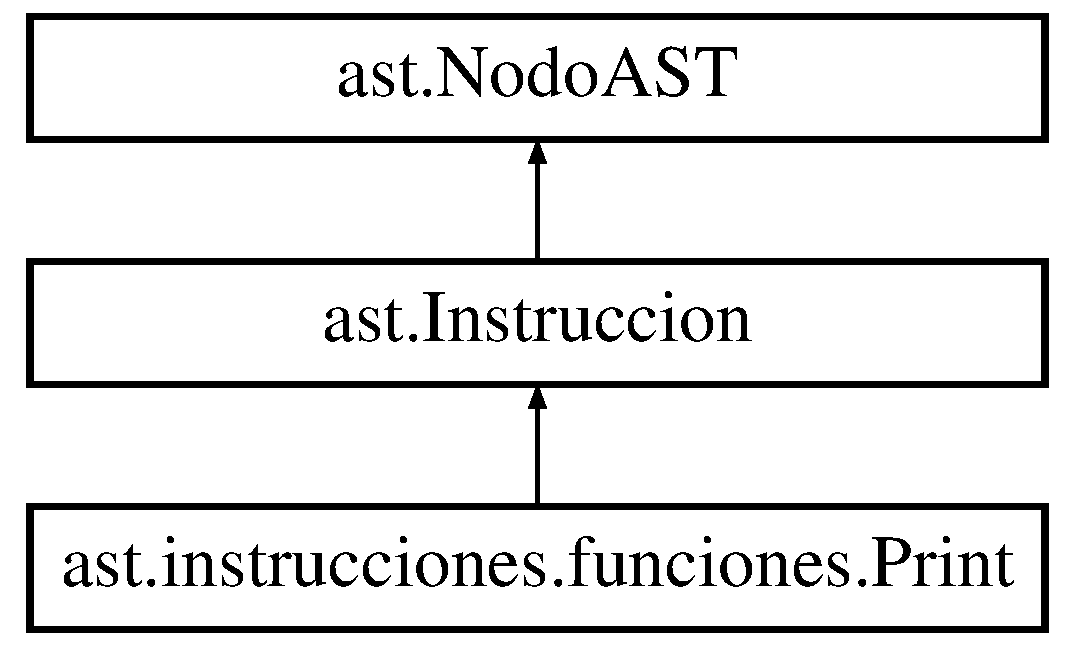
\includegraphics[height=3.000000cm]{classast_1_1instrucciones_1_1funciones_1_1_print}
\end{center}
\end{figure}
\subsection*{Public Member Functions}
\begin{DoxyCompactItemize}
\item 
\mbox{\Hypertarget{classast_1_1instrucciones_1_1funciones_1_1_print_add8316f296f8a793e597906f2874f7b0}\label{classast_1_1instrucciones_1_1funciones_1_1_print_add8316f296f8a793e597906f2874f7b0}} 
{\bfseries Print} (Linked\+List$<$ \mbox{\hyperlink{interfaceast_1_1_nodo_a_s_t}{Nodo\+A\+ST}} $>$ valor, int linea, int col)
\item 
\mbox{\Hypertarget{classast_1_1instrucciones_1_1funciones_1_1_print_aefe6b8b06145ac5e7ac367b839f2d861}\label{classast_1_1instrucciones_1_1funciones_1_1_print_aefe6b8b06145ac5e7ac367b839f2d861}} 
Object {\bfseries ejecutar} (\mbox{\hyperlink{classentorno_1_1_entorno}{Entorno}} ent)
\item 
\mbox{\Hypertarget{classast_1_1instrucciones_1_1funciones_1_1_print_a20f188614be38d425b4b42f35676673d}\label{classast_1_1instrucciones_1_1funciones_1_1_print_a20f188614be38d425b4b42f35676673d}} 
int {\bfseries linea} ()
\item 
\mbox{\Hypertarget{classast_1_1instrucciones_1_1funciones_1_1_print_a279e5c30d78d45262a9b46545c4da963}\label{classast_1_1instrucciones_1_1funciones_1_1_print_a279e5c30d78d45262a9b46545c4da963}} 
int {\bfseries columna} ()
\item 
\mbox{\Hypertarget{classast_1_1instrucciones_1_1funciones_1_1_print_a72e2d43be5f9cc22424a183e4f75b465}\label{classast_1_1instrucciones_1_1funciones_1_1_print_a72e2d43be5f9cc22424a183e4f75b465}} 
String {\bfseries get\+Nombre} (String\+Builder builder, String parent, int cont)
\end{DoxyCompactItemize}


\subsection{Detailed Description}
\begin{DoxyAuthor}{Author}
p\+\_\+ab1 
\end{DoxyAuthor}


The documentation for this class was generated from the following file\+:\begin{DoxyCompactItemize}
\item 
src/ast/instrucciones/funciones/Print.\+java\end{DoxyCompactItemize}

\hypertarget{classast_1_1expresiones_1_1operaciones_1_1_relacional}{}\section{ast.\+expresiones.\+operaciones.\+Relacional Class Reference}
\label{classast_1_1expresiones_1_1operaciones_1_1_relacional}\index{ast.\+expresiones.\+operaciones.\+Relacional@{ast.\+expresiones.\+operaciones.\+Relacional}}
Inheritance diagram for ast.\+expresiones.\+operaciones.\+Relacional\+:\begin{figure}[H]
\begin{center}
\leavevmode
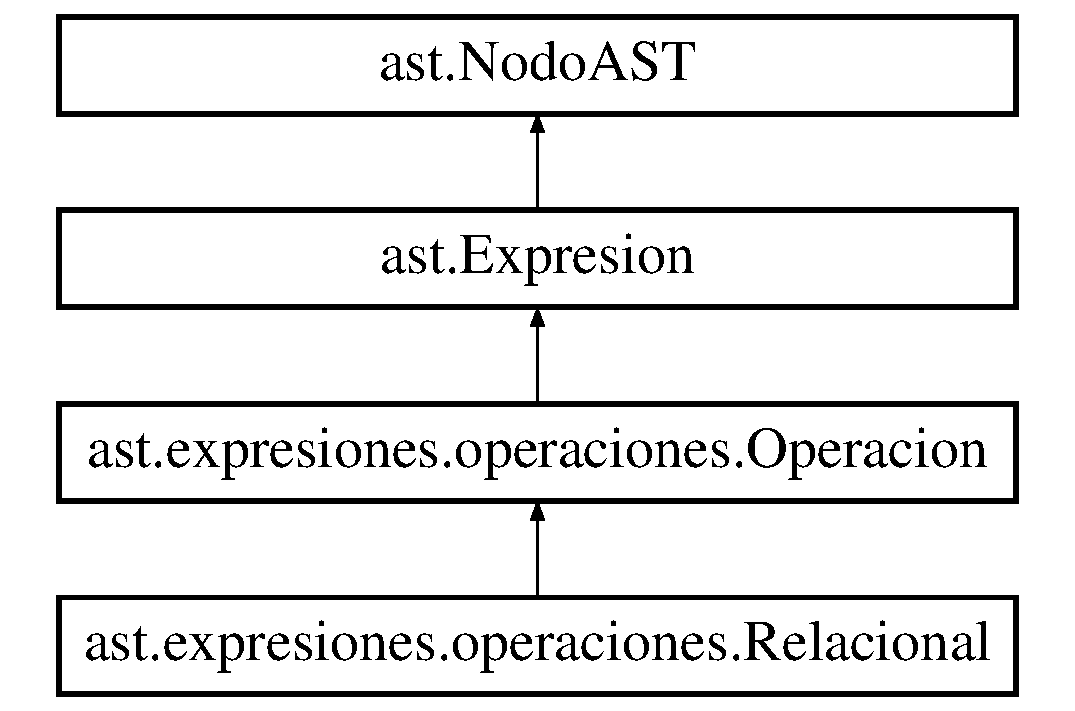
\includegraphics[height=4.000000cm]{classast_1_1expresiones_1_1operaciones_1_1_relacional}
\end{center}
\end{figure}
\subsection*{Public Member Functions}
\begin{DoxyCompactItemize}
\item 
\mbox{\Hypertarget{classast_1_1expresiones_1_1operaciones_1_1_relacional_affa7476b38b3736f30273f82004581d5}\label{classast_1_1expresiones_1_1operaciones_1_1_relacional_affa7476b38b3736f30273f82004581d5}} 
{\bfseries Relacional} (\mbox{\hyperlink{interfaceast_1_1_expresion}{Expresion}} op1, \mbox{\hyperlink{interfaceast_1_1_expresion}{Expresion}} op2, \mbox{\hyperlink{enumast_1_1expresiones_1_1operaciones_1_1_operacion_1_1_operador}{Operador}} operador, int col, int linea)
\item 
\mbox{\Hypertarget{classast_1_1expresiones_1_1operaciones_1_1_relacional_af74fb340d94f2360447571bd2c08598a}\label{classast_1_1expresiones_1_1operaciones_1_1_relacional_af74fb340d94f2360447571bd2c08598a}} 
\mbox{\hyperlink{classentorno_1_1_tipo}{Tipo}} {\bfseries tipo\+Dominante} (\mbox{\hyperlink{classentorno_1_1_tipo}{Tipo}} t1, \mbox{\hyperlink{classentorno_1_1_tipo}{Tipo}} t2)
\item 
\mbox{\Hypertarget{classast_1_1expresiones_1_1operaciones_1_1_relacional_aac8d5024ad8c235c1aff71e86e5424eb}\label{classast_1_1expresiones_1_1operaciones_1_1_relacional_aac8d5024ad8c235c1aff71e86e5424eb}} 
\mbox{\hyperlink{classentorno_1_1_tipo}{Tipo}} {\bfseries get\+Tipo} (\mbox{\hyperlink{classentorno_1_1_entorno}{Entorno}} ent)
\item 
\mbox{\Hypertarget{classast_1_1expresiones_1_1operaciones_1_1_relacional_a0ac356f08c68fd01fceddfaee94d8f94}\label{classast_1_1expresiones_1_1operaciones_1_1_relacional_a0ac356f08c68fd01fceddfaee94d8f94}} 
Object {\bfseries get\+Valor\+Implicito} (\mbox{\hyperlink{classentorno_1_1_entorno}{Entorno}} ent)
\item 
\mbox{\Hypertarget{classast_1_1expresiones_1_1operaciones_1_1_relacional_a6b2590ece1035e14f2924c9cdeaabe41}\label{classast_1_1expresiones_1_1operaciones_1_1_relacional_a6b2590ece1035e14f2924c9cdeaabe41}} 
String {\bfseries get\+Nombre} (String\+Builder builder, String parent, int cont)
\end{DoxyCompactItemize}


\subsection{Detailed Description}
\begin{DoxyAuthor}{Author}
p\+\_\+ab1 
\end{DoxyAuthor}


The documentation for this class was generated from the following file\+:\begin{DoxyCompactItemize}
\item 
src/ast/expresiones/operaciones/Relacional.\+java\end{DoxyCompactItemize}

\hypertarget{classast_1_1expresiones_1_1_return}{}\section{ast.\+expresiones.\+Return Class Reference}
\label{classast_1_1expresiones_1_1_return}\index{ast.\+expresiones.\+Return@{ast.\+expresiones.\+Return}}
Inheritance diagram for ast.\+expresiones.\+Return\+:\begin{figure}[H]
\begin{center}
\leavevmode
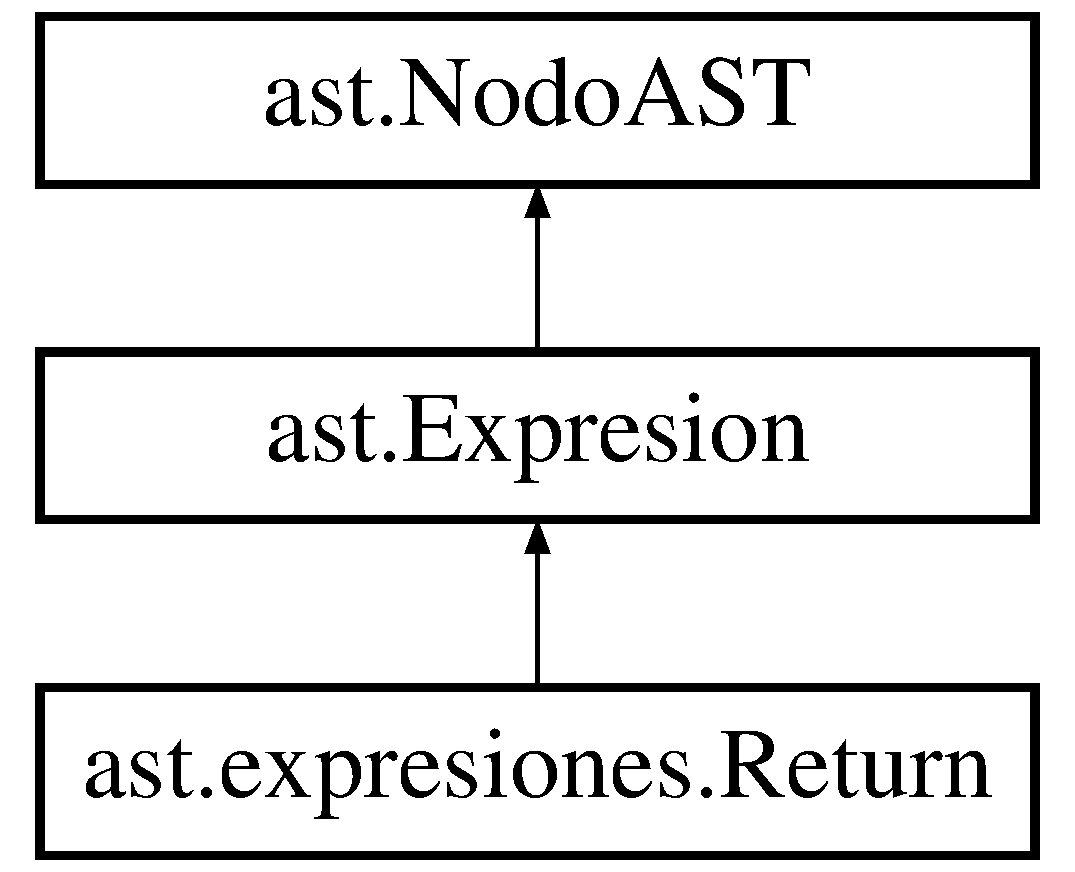
\includegraphics[height=3.000000cm]{classast_1_1expresiones_1_1_return}
\end{center}
\end{figure}
\subsection*{Public Member Functions}
\begin{DoxyCompactItemize}
\item 
\mbox{\Hypertarget{classast_1_1expresiones_1_1_return_a0edad8c4d216b655332c9c45bafb5869}\label{classast_1_1expresiones_1_1_return_a0edad8c4d216b655332c9c45bafb5869}} 
{\bfseries Return} (\mbox{\hyperlink{interfaceast_1_1_expresion}{Expresion}} valor\+De\+Retorno, int linea, int col)
\item 
\mbox{\Hypertarget{classast_1_1expresiones_1_1_return_a6fd9aa73203b52a8b59c73486b7c67e7}\label{classast_1_1expresiones_1_1_return_a6fd9aa73203b52a8b59c73486b7c67e7}} 
{\bfseries Return} (int linea, int col)
\item 
\mbox{\Hypertarget{classast_1_1expresiones_1_1_return_a9df47901353b0e95b77e02ae9f0c3681}\label{classast_1_1expresiones_1_1_return_a9df47901353b0e95b77e02ae9f0c3681}} 
boolean {\bfseries is\+Retorno\+Void} ()
\item 
\mbox{\Hypertarget{classast_1_1expresiones_1_1_return_ad667e0168d21509b6bf60e8adfafffbc}\label{classast_1_1expresiones_1_1_return_ad667e0168d21509b6bf60e8adfafffbc}} 
\mbox{\hyperlink{classentorno_1_1_tipo}{Tipo}} {\bfseries get\+Tipo} (\mbox{\hyperlink{classentorno_1_1_entorno}{Entorno}} ent)
\item 
\mbox{\Hypertarget{classast_1_1expresiones_1_1_return_a00d7e1d288717a291202480d75cc2a4c}\label{classast_1_1expresiones_1_1_return_a00d7e1d288717a291202480d75cc2a4c}} 
Object {\bfseries get\+Valor\+Implicito} (\mbox{\hyperlink{classentorno_1_1_entorno}{Entorno}} ent)
\item 
\mbox{\Hypertarget{classast_1_1expresiones_1_1_return_adae64964aa7ae224cf146349a3689e6a}\label{classast_1_1expresiones_1_1_return_adae64964aa7ae224cf146349a3689e6a}} 
int {\bfseries linea} ()
\item 
\mbox{\Hypertarget{classast_1_1expresiones_1_1_return_a503b256fb62db81f0080573d129eab17}\label{classast_1_1expresiones_1_1_return_a503b256fb62db81f0080573d129eab17}} 
int {\bfseries columna} ()
\item 
\mbox{\Hypertarget{classast_1_1expresiones_1_1_return_aae6bde9860f51ec171be9b75e2671d4f}\label{classast_1_1expresiones_1_1_return_aae6bde9860f51ec171be9b75e2671d4f}} 
String {\bfseries get\+Nombre} (String\+Builder builder, String parent, int cont)
\end{DoxyCompactItemize}


\subsection{Detailed Description}
\begin{DoxyAuthor}{Author}
p\+\_\+ab1 
\end{DoxyAuthor}


The documentation for this class was generated from the following file\+:\begin{DoxyCompactItemize}
\item 
src/ast/expresiones/Return.\+java\end{DoxyCompactItemize}

\hypertarget{enumentorno_1_1_simbolo_1_1_rol}{}\section{entorno.\+Simbolo.\+Rol Enum Reference}
\label{enumentorno_1_1_simbolo_1_1_rol}\index{entorno.\+Simbolo.\+Rol@{entorno.\+Simbolo.\+Rol}}
\subsection*{Public Attributes}
\begin{DoxyCompactItemize}
\item 
\mbox{\Hypertarget{enumentorno_1_1_simbolo_1_1_rol_af428d7bec6529ef5a3b296225451c26d}\label{enumentorno_1_1_simbolo_1_1_rol_af428d7bec6529ef5a3b296225451c26d}} 
{\bfseries V\+E\+C\+T\+OR}
\item 
\mbox{\Hypertarget{enumentorno_1_1_simbolo_1_1_rol_ace161dc961bb736c942e56a47b601a79}\label{enumentorno_1_1_simbolo_1_1_rol_ace161dc961bb736c942e56a47b601a79}} 
{\bfseries L\+I\+S\+TA}
\item 
\mbox{\Hypertarget{enumentorno_1_1_simbolo_1_1_rol_a21b1b81d4f8b607bcd7d3ba86b4dbc82}\label{enumentorno_1_1_simbolo_1_1_rol_a21b1b81d4f8b607bcd7d3ba86b4dbc82}} 
{\bfseries M\+A\+T\+R\+IZ}
\item 
\mbox{\Hypertarget{enumentorno_1_1_simbolo_1_1_rol_a54c9d8bb3fbc8cf54de4f2aa70f70007}\label{enumentorno_1_1_simbolo_1_1_rol_a54c9d8bb3fbc8cf54de4f2aa70f70007}} 
{\bfseries A\+R\+R\+E\+G\+LO}
\item 
\mbox{\Hypertarget{enumentorno_1_1_simbolo_1_1_rol_ade66cf36298c14a69dd9f9d9c619fb93}\label{enumentorno_1_1_simbolo_1_1_rol_ade66cf36298c14a69dd9f9d9c619fb93}} 
{\bfseries F\+U\+N\+C\+I\+ON}
\end{DoxyCompactItemize}


The documentation for this enum was generated from the following file\+:\begin{DoxyCompactItemize}
\item 
src/entorno/Simbolo.\+java\end{DoxyCompactItemize}

\hypertarget{classentorno_1_1_simbolo}{}\section{entorno.\+Simbolo Class Reference}
\label{classentorno_1_1_simbolo}\index{entorno.\+Simbolo@{entorno.\+Simbolo}}
Inheritance diagram for entorno.\+Simbolo\+:\begin{figure}[H]
\begin{center}
\leavevmode
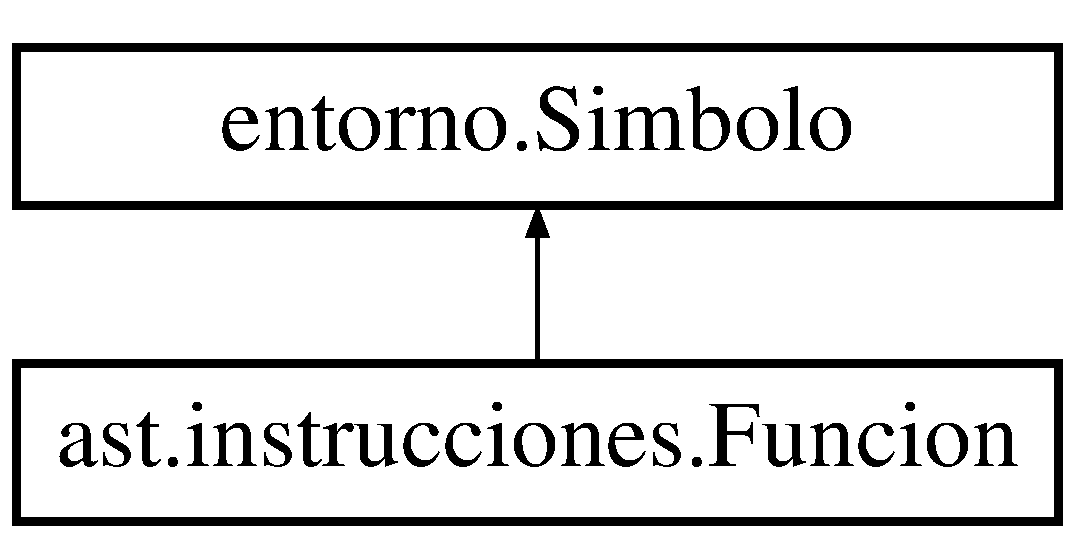
\includegraphics[height=2.000000cm]{classentorno_1_1_simbolo}
\end{center}
\end{figure}
\subsection*{Classes}
\begin{DoxyCompactItemize}
\item 
enum \mbox{\hyperlink{enumentorno_1_1_simbolo_1_1_acc}{Acc}}
\item 
enum \mbox{\hyperlink{enumentorno_1_1_simbolo_1_1_rol}{Rol}}
\end{DoxyCompactItemize}
\subsection*{Public Member Functions}
\begin{DoxyCompactItemize}
\item 
\mbox{\Hypertarget{classentorno_1_1_simbolo_ad95d1f480f166dd64e878a9779828cd6}\label{classentorno_1_1_simbolo_ad95d1f480f166dd64e878a9779828cd6}} 
{\bfseries Simbolo} (String identificador, Object valor, \mbox{\hyperlink{classentorno_1_1_tipo}{Tipo}} tipo, \mbox{\hyperlink{enumentorno_1_1_simbolo_1_1_rol}{Rol}} rol, int dim)
\item 
\mbox{\Hypertarget{classentorno_1_1_simbolo_aed7f5e07a79ac062383fe1876abce7b6}\label{classentorno_1_1_simbolo_aed7f5e07a79ac062383fe1876abce7b6}} 
{\bfseries Simbolo} (String id, \mbox{\hyperlink{enumentorno_1_1_simbolo_1_1_rol}{Rol}} rol)
\item 
\mbox{\Hypertarget{classentorno_1_1_simbolo_a5501bd67507a8372fd97e1e6d5c0ac20}\label{classentorno_1_1_simbolo_a5501bd67507a8372fd97e1e6d5c0ac20}} 
{\bfseries Simbolo} (String id, \mbox{\hyperlink{enumentorno_1_1_simbolo_1_1_rol}{Rol}} rol, Object valor)
\item 
\mbox{\Hypertarget{classentorno_1_1_simbolo_a4960314d68f6ef105fdfcf3489812227}\label{classentorno_1_1_simbolo_a4960314d68f6ef105fdfcf3489812227}} 
String {\bfseries get\+Identificador} ()
\item 
\mbox{\Hypertarget{classentorno_1_1_simbolo_a31e199ddb428936fbf33e25d6e69e3d5}\label{classentorno_1_1_simbolo_a31e199ddb428936fbf33e25d6e69e3d5}} 
void {\bfseries set\+Identificador} (String identificador)
\item 
\mbox{\Hypertarget{classentorno_1_1_simbolo_a129b6aec61c7bfcecb84fffa721846be}\label{classentorno_1_1_simbolo_a129b6aec61c7bfcecb84fffa721846be}} 
Object {\bfseries get\+Valor} ()
\item 
\mbox{\Hypertarget{classentorno_1_1_simbolo_a1df1e0af8018c9d58702c1c6c4cc5325}\label{classentorno_1_1_simbolo_a1df1e0af8018c9d58702c1c6c4cc5325}} 
void {\bfseries set\+Valor} (Object valor)
\item 
\mbox{\Hypertarget{classentorno_1_1_simbolo_a852e60225ce617f81537f77cc6bf7eb4}\label{classentorno_1_1_simbolo_a852e60225ce617f81537f77cc6bf7eb4}} 
\mbox{\hyperlink{classentorno_1_1_tipo}{Tipo}} {\bfseries get\+Tipo} ()
\item 
\mbox{\Hypertarget{classentorno_1_1_simbolo_ad3df2118aa22e27caa80896fd27f9862}\label{classentorno_1_1_simbolo_ad3df2118aa22e27caa80896fd27f9862}} 
void {\bfseries set\+Tipo} (\mbox{\hyperlink{classentorno_1_1_tipo}{Tipo}} tipo)
\item 
\mbox{\Hypertarget{classentorno_1_1_simbolo_a939cdbdf8d27e795ad2eb4697c8f3e5e}\label{classentorno_1_1_simbolo_a939cdbdf8d27e795ad2eb4697c8f3e5e}} 
\mbox{\hyperlink{enumentorno_1_1_simbolo_1_1_rol}{Rol}} {\bfseries get\+Rol} ()
\item 
\mbox{\Hypertarget{classentorno_1_1_simbolo_a52c0e3d4026fd78e28f0deab6062142c}\label{classentorno_1_1_simbolo_a52c0e3d4026fd78e28f0deab6062142c}} 
void {\bfseries set\+Rol} (\mbox{\hyperlink{enumentorno_1_1_simbolo_1_1_rol}{Rol}} rol)
\end{DoxyCompactItemize}
\subsection*{Public Attributes}
\begin{DoxyCompactItemize}
\item 
\mbox{\Hypertarget{classentorno_1_1_simbolo_a26bbe6ff1d532cc556594e89034b41bb}\label{classentorno_1_1_simbolo_a26bbe6ff1d532cc556594e89034b41bb}} 
int {\bfseries lugar}
\end{DoxyCompactItemize}


\subsection{Detailed Description}
\begin{DoxyAuthor}{Author}
p\+\_\+ab1 
\end{DoxyAuthor}


The documentation for this class was generated from the following file\+:\begin{DoxyCompactItemize}
\item 
src/entorno/Simbolo.\+java\end{DoxyCompactItemize}

\hypertarget{classanalizadores_1_1_simple_char_stream}{}\section{analizadores.\+Simple\+Char\+Stream Class Reference}
\label{classanalizadores_1_1_simple_char_stream}\index{analizadores.\+Simple\+Char\+Stream@{analizadores.\+Simple\+Char\+Stream}}
\subsection*{Public Member Functions}
\begin{DoxyCompactItemize}
\item 
char \mbox{\hyperlink{classanalizadores_1_1_simple_char_stream_a5b71e22435880e75608126903932096b}{Begin\+Token}} ()  throws java.\+io.\+I\+O\+Exception   
\item 
char \mbox{\hyperlink{classanalizadores_1_1_simple_char_stream_a9464412a320a813e875a461e6b0bb2af}{read\+Char}} ()  throws java.\+io.\+I\+O\+Exception   
\item 
int \mbox{\hyperlink{classanalizadores_1_1_simple_char_stream_ad9fd1239a7ecd61c0106e6863d8f81cd}{get\+Column}} ()
\item 
int \mbox{\hyperlink{classanalizadores_1_1_simple_char_stream_ad2af5c3f4fadce0ec36b08eb5bc67b42}{get\+Line}} ()
\item 
int \mbox{\hyperlink{classanalizadores_1_1_simple_char_stream_a3ab1da641448601061ce9a7ebea34708}{get\+End\+Column}} ()
\item 
int \mbox{\hyperlink{classanalizadores_1_1_simple_char_stream_a3fdfd0491baacd797c687589159c7a98}{get\+End\+Line}} ()
\item 
int \mbox{\hyperlink{classanalizadores_1_1_simple_char_stream_af5e3275258c76e84e09cde45971d2c6f}{get\+Begin\+Column}} ()
\item 
int \mbox{\hyperlink{classanalizadores_1_1_simple_char_stream_a161f2eda40737765b89e9d0c28decadf}{get\+Begin\+Line}} ()
\item 
void \mbox{\hyperlink{classanalizadores_1_1_simple_char_stream_a63dfe525e3f73ea9277581d0e8853d1a}{backup}} (int amount)
\item 
\mbox{\hyperlink{classanalizadores_1_1_simple_char_stream_a6debcff3bab58fc04e50fea277eddda6}{Simple\+Char\+Stream}} (java.\+io.\+Reader dstream, int startline, int startcolumn, int buffersize)
\item 
\mbox{\hyperlink{classanalizadores_1_1_simple_char_stream_abd26499c5e2b7106edb3ce04085f5603}{Simple\+Char\+Stream}} (java.\+io.\+Reader dstream, int startline, int startcolumn)
\item 
\mbox{\hyperlink{classanalizadores_1_1_simple_char_stream_a8cf5c59abc089551cf182a074481cfad}{Simple\+Char\+Stream}} (java.\+io.\+Reader dstream)
\item 
void \mbox{\hyperlink{classanalizadores_1_1_simple_char_stream_a244de250f7d2c63115e0b9dd7edf27d7}{Re\+Init}} (java.\+io.\+Reader dstream, int startline, int startcolumn, int buffersize)
\item 
void \mbox{\hyperlink{classanalizadores_1_1_simple_char_stream_ad88c7f702fffeae097e1bbae81601894}{Re\+Init}} (java.\+io.\+Reader dstream, int startline, int startcolumn)
\item 
void \mbox{\hyperlink{classanalizadores_1_1_simple_char_stream_a1c531cf74a9047ec165d25e6b2b6a428}{Re\+Init}} (java.\+io.\+Reader dstream)
\item 
\mbox{\hyperlink{classanalizadores_1_1_simple_char_stream_a2f543453e34d9d15876263693c2f1ffe}{Simple\+Char\+Stream}} (java.\+io.\+Input\+Stream dstream, String encoding, int startline, int startcolumn, int buffersize)  throws java.\+io.\+Unsupported\+Encoding\+Exception   
\item 
\mbox{\hyperlink{classanalizadores_1_1_simple_char_stream_ac3d2c52438f4d29440590c61b9c321f0}{Simple\+Char\+Stream}} (java.\+io.\+Input\+Stream dstream, int startline, int startcolumn, int buffersize)
\item 
\mbox{\hyperlink{classanalizadores_1_1_simple_char_stream_a277db3968e8f2b76a24f6d90ea9942d9}{Simple\+Char\+Stream}} (java.\+io.\+Input\+Stream dstream, String encoding, int startline, int startcolumn)  throws java.\+io.\+Unsupported\+Encoding\+Exception   
\item 
\mbox{\hyperlink{classanalizadores_1_1_simple_char_stream_a7ffee5e3a468a82be8d5b35933bd9ab0}{Simple\+Char\+Stream}} (java.\+io.\+Input\+Stream dstream, int startline, int startcolumn)
\item 
\mbox{\hyperlink{classanalizadores_1_1_simple_char_stream_a08a7b1c3bc75056cc19bdbcc1ac42306}{Simple\+Char\+Stream}} (java.\+io.\+Input\+Stream dstream, String encoding)  throws java.\+io.\+Unsupported\+Encoding\+Exception   
\item 
\mbox{\hyperlink{classanalizadores_1_1_simple_char_stream_aa148a7b81b78a16ddf2a120531d189cb}{Simple\+Char\+Stream}} (java.\+io.\+Input\+Stream dstream)
\item 
void \mbox{\hyperlink{classanalizadores_1_1_simple_char_stream_aec69ff69d9dfc99d8c011e430107a90a}{Re\+Init}} (java.\+io.\+Input\+Stream dstream, String encoding, int startline, int startcolumn, int buffersize)  throws java.\+io.\+Unsupported\+Encoding\+Exception   
\item 
void \mbox{\hyperlink{classanalizadores_1_1_simple_char_stream_a539ab799edc2ed4fb47f9610d6328393}{Re\+Init}} (java.\+io.\+Input\+Stream dstream, int startline, int startcolumn, int buffersize)
\item 
void \mbox{\hyperlink{classanalizadores_1_1_simple_char_stream_a947f68635529dd654e982b65b250432a}{Re\+Init}} (java.\+io.\+Input\+Stream dstream, String encoding)  throws java.\+io.\+Unsupported\+Encoding\+Exception   
\item 
void \mbox{\hyperlink{classanalizadores_1_1_simple_char_stream_a3fc08691c124d2c6c9dd1f5edfbc1fd3}{Re\+Init}} (java.\+io.\+Input\+Stream dstream)
\item 
void \mbox{\hyperlink{classanalizadores_1_1_simple_char_stream_acd17c0194c5b3d2b3506782e57793e78}{Re\+Init}} (java.\+io.\+Input\+Stream dstream, String encoding, int startline, int startcolumn)  throws java.\+io.\+Unsupported\+Encoding\+Exception   
\item 
void \mbox{\hyperlink{classanalizadores_1_1_simple_char_stream_ae94f07895d46eb432af5b6f43a20630b}{Re\+Init}} (java.\+io.\+Input\+Stream dstream, int startline, int startcolumn)
\item 
String \mbox{\hyperlink{classanalizadores_1_1_simple_char_stream_aeb5b88a70873ad9cc35763622397b6f2}{Get\+Image}} ()
\item 
char \mbox{[}$\,$\mbox{]} \mbox{\hyperlink{classanalizadores_1_1_simple_char_stream_a3312f3c97f5b1b00635960754d1fc777}{Get\+Suffix}} (int len)
\item 
void \mbox{\hyperlink{classanalizadores_1_1_simple_char_stream_a4760af11a45ce9451c5bc1b43d1e48fc}{Done}} ()
\item 
void \mbox{\hyperlink{classanalizadores_1_1_simple_char_stream_a108c5d7d6556c924a0cacd480e9860e1}{adjust\+Begin\+Line\+Column}} (int new\+Line, int new\+Col)
\end{DoxyCompactItemize}
\subsection*{Public Attributes}
\begin{DoxyCompactItemize}
\item 
int \mbox{\hyperlink{classanalizadores_1_1_simple_char_stream_ae6a80a1bd35bee86088babe7ff27b68a}{bufpos}} = -\/1
\end{DoxyCompactItemize}
\subsection*{Static Public Attributes}
\begin{DoxyCompactItemize}
\item 
static final boolean \mbox{\hyperlink{classanalizadores_1_1_simple_char_stream_a3099cb81a656d590a7a974110326af9e}{static\+Flag}} = false
\end{DoxyCompactItemize}
\subsection*{Protected Member Functions}
\begin{DoxyCompactItemize}
\item 
\mbox{\Hypertarget{classanalizadores_1_1_simple_char_stream_a541362a1fae4e62732c33646661a1321}\label{classanalizadores_1_1_simple_char_stream_a541362a1fae4e62732c33646661a1321}} 
void {\bfseries set\+Tab\+Size} (int i)
\item 
\mbox{\Hypertarget{classanalizadores_1_1_simple_char_stream_a45e004117b5fd71f0849d81c28889899}\label{classanalizadores_1_1_simple_char_stream_a45e004117b5fd71f0849d81c28889899}} 
int {\bfseries get\+Tab\+Size} (int i)
\item 
\mbox{\Hypertarget{classanalizadores_1_1_simple_char_stream_a58b4fbb1ce2d8d6373aebe1f123c277e}\label{classanalizadores_1_1_simple_char_stream_a58b4fbb1ce2d8d6373aebe1f123c277e}} 
void {\bfseries Expand\+Buff} (boolean wrap\+Around)
\item 
\mbox{\Hypertarget{classanalizadores_1_1_simple_char_stream_a31af0e9c3b2b4dd07cc37bc16025fcd5}\label{classanalizadores_1_1_simple_char_stream_a31af0e9c3b2b4dd07cc37bc16025fcd5}} 
void {\bfseries Fill\+Buff} ()  throws java.\+io.\+I\+O\+Exception   
\item 
\mbox{\Hypertarget{classanalizadores_1_1_simple_char_stream_a53d68dbbb05497d957c821a210b069ba}\label{classanalizadores_1_1_simple_char_stream_a53d68dbbb05497d957c821a210b069ba}} 
void {\bfseries Update\+Line\+Column} (char c)
\end{DoxyCompactItemize}
\subsection*{Protected Attributes}
\begin{DoxyCompactItemize}
\item 
\mbox{\Hypertarget{classanalizadores_1_1_simple_char_stream_a468980f757dcb20685ab3b6eb29dce83}\label{classanalizadores_1_1_simple_char_stream_a468980f757dcb20685ab3b6eb29dce83}} 
int {\bfseries bufline} \mbox{[}$\,$\mbox{]}
\item 
\mbox{\Hypertarget{classanalizadores_1_1_simple_char_stream_a2004aa422613d16258dbb9782335f584}\label{classanalizadores_1_1_simple_char_stream_a2004aa422613d16258dbb9782335f584}} 
int {\bfseries bufcolumn} \mbox{[}$\,$\mbox{]}
\item 
\mbox{\Hypertarget{classanalizadores_1_1_simple_char_stream_a72705073194f3f0c2067b9f59a1d56ee}\label{classanalizadores_1_1_simple_char_stream_a72705073194f3f0c2067b9f59a1d56ee}} 
int {\bfseries column} = 0
\item 
\mbox{\Hypertarget{classanalizadores_1_1_simple_char_stream_a0e9e3ff855f35427108e02057a25d01e}\label{classanalizadores_1_1_simple_char_stream_a0e9e3ff855f35427108e02057a25d01e}} 
int {\bfseries line} = 1
\item 
\mbox{\Hypertarget{classanalizadores_1_1_simple_char_stream_a8cf04171b13cd01abd88e92f0edd4335}\label{classanalizadores_1_1_simple_char_stream_a8cf04171b13cd01abd88e92f0edd4335}} 
boolean {\bfseries prev\+Char\+Is\+CR} = false
\item 
\mbox{\Hypertarget{classanalizadores_1_1_simple_char_stream_a5fd7e22850ab17176d2a1107ccf4fbac}\label{classanalizadores_1_1_simple_char_stream_a5fd7e22850ab17176d2a1107ccf4fbac}} 
boolean {\bfseries prev\+Char\+Is\+LF} = false
\item 
\mbox{\Hypertarget{classanalizadores_1_1_simple_char_stream_a90c2b1728935e512de8c68c1d257a074}\label{classanalizadores_1_1_simple_char_stream_a90c2b1728935e512de8c68c1d257a074}} 
java.\+io.\+Reader {\bfseries input\+Stream}
\item 
\mbox{\Hypertarget{classanalizadores_1_1_simple_char_stream_ae01d1c8d66207976a7d5a0933d700c1e}\label{classanalizadores_1_1_simple_char_stream_ae01d1c8d66207976a7d5a0933d700c1e}} 
char \mbox{[}$\,$\mbox{]} {\bfseries buffer}
\item 
\mbox{\Hypertarget{classanalizadores_1_1_simple_char_stream_a53b5143ed21976b4aa93801f93eaec79}\label{classanalizadores_1_1_simple_char_stream_a53b5143ed21976b4aa93801f93eaec79}} 
int {\bfseries max\+Next\+Char\+Ind} = 0
\item 
\mbox{\Hypertarget{classanalizadores_1_1_simple_char_stream_a85e7c0dcafe3473bdc0d3d0806b907dc}\label{classanalizadores_1_1_simple_char_stream_a85e7c0dcafe3473bdc0d3d0806b907dc}} 
int {\bfseries in\+Buf} = 0
\item 
\mbox{\Hypertarget{classanalizadores_1_1_simple_char_stream_a24c0e4778d79d034e3ba3336e8a32c2d}\label{classanalizadores_1_1_simple_char_stream_a24c0e4778d79d034e3ba3336e8a32c2d}} 
int {\bfseries tab\+Size} = 8
\end{DoxyCompactItemize}


\subsection{Detailed Description}
An implementation of interface Char\+Stream, where the stream is assumed to contain only A\+S\+C\+II characters (without unicode processing). 

\subsection{Constructor \& Destructor Documentation}
\mbox{\Hypertarget{classanalizadores_1_1_simple_char_stream_a6debcff3bab58fc04e50fea277eddda6}\label{classanalizadores_1_1_simple_char_stream_a6debcff3bab58fc04e50fea277eddda6}} 
\index{analizadores\+::\+Simple\+Char\+Stream@{analizadores\+::\+Simple\+Char\+Stream}!Simple\+Char\+Stream@{Simple\+Char\+Stream}}
\index{Simple\+Char\+Stream@{Simple\+Char\+Stream}!analizadores\+::\+Simple\+Char\+Stream@{analizadores\+::\+Simple\+Char\+Stream}}
\subsubsection{\texorpdfstring{Simple\+Char\+Stream()}{SimpleCharStream()}\hspace{0.1cm}{\footnotesize\ttfamily [1/9]}}
{\footnotesize\ttfamily analizadores.\+Simple\+Char\+Stream.\+Simple\+Char\+Stream (\begin{DoxyParamCaption}\item[{java.\+io.\+Reader}]{dstream,  }\item[{int}]{startline,  }\item[{int}]{startcolumn,  }\item[{int}]{buffersize }\end{DoxyParamCaption})}

Constructor. \mbox{\Hypertarget{classanalizadores_1_1_simple_char_stream_abd26499c5e2b7106edb3ce04085f5603}\label{classanalizadores_1_1_simple_char_stream_abd26499c5e2b7106edb3ce04085f5603}} 
\index{analizadores\+::\+Simple\+Char\+Stream@{analizadores\+::\+Simple\+Char\+Stream}!Simple\+Char\+Stream@{Simple\+Char\+Stream}}
\index{Simple\+Char\+Stream@{Simple\+Char\+Stream}!analizadores\+::\+Simple\+Char\+Stream@{analizadores\+::\+Simple\+Char\+Stream}}
\subsubsection{\texorpdfstring{Simple\+Char\+Stream()}{SimpleCharStream()}\hspace{0.1cm}{\footnotesize\ttfamily [2/9]}}
{\footnotesize\ttfamily analizadores.\+Simple\+Char\+Stream.\+Simple\+Char\+Stream (\begin{DoxyParamCaption}\item[{java.\+io.\+Reader}]{dstream,  }\item[{int}]{startline,  }\item[{int}]{startcolumn }\end{DoxyParamCaption})}

Constructor. \mbox{\Hypertarget{classanalizadores_1_1_simple_char_stream_a8cf5c59abc089551cf182a074481cfad}\label{classanalizadores_1_1_simple_char_stream_a8cf5c59abc089551cf182a074481cfad}} 
\index{analizadores\+::\+Simple\+Char\+Stream@{analizadores\+::\+Simple\+Char\+Stream}!Simple\+Char\+Stream@{Simple\+Char\+Stream}}
\index{Simple\+Char\+Stream@{Simple\+Char\+Stream}!analizadores\+::\+Simple\+Char\+Stream@{analizadores\+::\+Simple\+Char\+Stream}}
\subsubsection{\texorpdfstring{Simple\+Char\+Stream()}{SimpleCharStream()}\hspace{0.1cm}{\footnotesize\ttfamily [3/9]}}
{\footnotesize\ttfamily analizadores.\+Simple\+Char\+Stream.\+Simple\+Char\+Stream (\begin{DoxyParamCaption}\item[{java.\+io.\+Reader}]{dstream }\end{DoxyParamCaption})}

Constructor. \mbox{\Hypertarget{classanalizadores_1_1_simple_char_stream_a2f543453e34d9d15876263693c2f1ffe}\label{classanalizadores_1_1_simple_char_stream_a2f543453e34d9d15876263693c2f1ffe}} 
\index{analizadores\+::\+Simple\+Char\+Stream@{analizadores\+::\+Simple\+Char\+Stream}!Simple\+Char\+Stream@{Simple\+Char\+Stream}}
\index{Simple\+Char\+Stream@{Simple\+Char\+Stream}!analizadores\+::\+Simple\+Char\+Stream@{analizadores\+::\+Simple\+Char\+Stream}}
\subsubsection{\texorpdfstring{Simple\+Char\+Stream()}{SimpleCharStream()}\hspace{0.1cm}{\footnotesize\ttfamily [4/9]}}
{\footnotesize\ttfamily analizadores.\+Simple\+Char\+Stream.\+Simple\+Char\+Stream (\begin{DoxyParamCaption}\item[{java.\+io.\+Input\+Stream}]{dstream,  }\item[{String}]{encoding,  }\item[{int}]{startline,  }\item[{int}]{startcolumn,  }\item[{int}]{buffersize }\end{DoxyParamCaption}) throws java.\+io.\+Unsupported\+Encoding\+Exception}

Constructor. \mbox{\Hypertarget{classanalizadores_1_1_simple_char_stream_ac3d2c52438f4d29440590c61b9c321f0}\label{classanalizadores_1_1_simple_char_stream_ac3d2c52438f4d29440590c61b9c321f0}} 
\index{analizadores\+::\+Simple\+Char\+Stream@{analizadores\+::\+Simple\+Char\+Stream}!Simple\+Char\+Stream@{Simple\+Char\+Stream}}
\index{Simple\+Char\+Stream@{Simple\+Char\+Stream}!analizadores\+::\+Simple\+Char\+Stream@{analizadores\+::\+Simple\+Char\+Stream}}
\subsubsection{\texorpdfstring{Simple\+Char\+Stream()}{SimpleCharStream()}\hspace{0.1cm}{\footnotesize\ttfamily [5/9]}}
{\footnotesize\ttfamily analizadores.\+Simple\+Char\+Stream.\+Simple\+Char\+Stream (\begin{DoxyParamCaption}\item[{java.\+io.\+Input\+Stream}]{dstream,  }\item[{int}]{startline,  }\item[{int}]{startcolumn,  }\item[{int}]{buffersize }\end{DoxyParamCaption})}

Constructor. \mbox{\Hypertarget{classanalizadores_1_1_simple_char_stream_a277db3968e8f2b76a24f6d90ea9942d9}\label{classanalizadores_1_1_simple_char_stream_a277db3968e8f2b76a24f6d90ea9942d9}} 
\index{analizadores\+::\+Simple\+Char\+Stream@{analizadores\+::\+Simple\+Char\+Stream}!Simple\+Char\+Stream@{Simple\+Char\+Stream}}
\index{Simple\+Char\+Stream@{Simple\+Char\+Stream}!analizadores\+::\+Simple\+Char\+Stream@{analizadores\+::\+Simple\+Char\+Stream}}
\subsubsection{\texorpdfstring{Simple\+Char\+Stream()}{SimpleCharStream()}\hspace{0.1cm}{\footnotesize\ttfamily [6/9]}}
{\footnotesize\ttfamily analizadores.\+Simple\+Char\+Stream.\+Simple\+Char\+Stream (\begin{DoxyParamCaption}\item[{java.\+io.\+Input\+Stream}]{dstream,  }\item[{String}]{encoding,  }\item[{int}]{startline,  }\item[{int}]{startcolumn }\end{DoxyParamCaption}) throws java.\+io.\+Unsupported\+Encoding\+Exception}

Constructor. \mbox{\Hypertarget{classanalizadores_1_1_simple_char_stream_a7ffee5e3a468a82be8d5b35933bd9ab0}\label{classanalizadores_1_1_simple_char_stream_a7ffee5e3a468a82be8d5b35933bd9ab0}} 
\index{analizadores\+::\+Simple\+Char\+Stream@{analizadores\+::\+Simple\+Char\+Stream}!Simple\+Char\+Stream@{Simple\+Char\+Stream}}
\index{Simple\+Char\+Stream@{Simple\+Char\+Stream}!analizadores\+::\+Simple\+Char\+Stream@{analizadores\+::\+Simple\+Char\+Stream}}
\subsubsection{\texorpdfstring{Simple\+Char\+Stream()}{SimpleCharStream()}\hspace{0.1cm}{\footnotesize\ttfamily [7/9]}}
{\footnotesize\ttfamily analizadores.\+Simple\+Char\+Stream.\+Simple\+Char\+Stream (\begin{DoxyParamCaption}\item[{java.\+io.\+Input\+Stream}]{dstream,  }\item[{int}]{startline,  }\item[{int}]{startcolumn }\end{DoxyParamCaption})}

Constructor. \mbox{\Hypertarget{classanalizadores_1_1_simple_char_stream_a08a7b1c3bc75056cc19bdbcc1ac42306}\label{classanalizadores_1_1_simple_char_stream_a08a7b1c3bc75056cc19bdbcc1ac42306}} 
\index{analizadores\+::\+Simple\+Char\+Stream@{analizadores\+::\+Simple\+Char\+Stream}!Simple\+Char\+Stream@{Simple\+Char\+Stream}}
\index{Simple\+Char\+Stream@{Simple\+Char\+Stream}!analizadores\+::\+Simple\+Char\+Stream@{analizadores\+::\+Simple\+Char\+Stream}}
\subsubsection{\texorpdfstring{Simple\+Char\+Stream()}{SimpleCharStream()}\hspace{0.1cm}{\footnotesize\ttfamily [8/9]}}
{\footnotesize\ttfamily analizadores.\+Simple\+Char\+Stream.\+Simple\+Char\+Stream (\begin{DoxyParamCaption}\item[{java.\+io.\+Input\+Stream}]{dstream,  }\item[{String}]{encoding }\end{DoxyParamCaption}) throws java.\+io.\+Unsupported\+Encoding\+Exception}

Constructor. \mbox{\Hypertarget{classanalizadores_1_1_simple_char_stream_aa148a7b81b78a16ddf2a120531d189cb}\label{classanalizadores_1_1_simple_char_stream_aa148a7b81b78a16ddf2a120531d189cb}} 
\index{analizadores\+::\+Simple\+Char\+Stream@{analizadores\+::\+Simple\+Char\+Stream}!Simple\+Char\+Stream@{Simple\+Char\+Stream}}
\index{Simple\+Char\+Stream@{Simple\+Char\+Stream}!analizadores\+::\+Simple\+Char\+Stream@{analizadores\+::\+Simple\+Char\+Stream}}
\subsubsection{\texorpdfstring{Simple\+Char\+Stream()}{SimpleCharStream()}\hspace{0.1cm}{\footnotesize\ttfamily [9/9]}}
{\footnotesize\ttfamily analizadores.\+Simple\+Char\+Stream.\+Simple\+Char\+Stream (\begin{DoxyParamCaption}\item[{java.\+io.\+Input\+Stream}]{dstream }\end{DoxyParamCaption})}

Constructor. 

\subsection{Member Function Documentation}
\mbox{\Hypertarget{classanalizadores_1_1_simple_char_stream_a108c5d7d6556c924a0cacd480e9860e1}\label{classanalizadores_1_1_simple_char_stream_a108c5d7d6556c924a0cacd480e9860e1}} 
\index{analizadores\+::\+Simple\+Char\+Stream@{analizadores\+::\+Simple\+Char\+Stream}!adjust\+Begin\+Line\+Column@{adjust\+Begin\+Line\+Column}}
\index{adjust\+Begin\+Line\+Column@{adjust\+Begin\+Line\+Column}!analizadores\+::\+Simple\+Char\+Stream@{analizadores\+::\+Simple\+Char\+Stream}}
\subsubsection{\texorpdfstring{adjust\+Begin\+Line\+Column()}{adjustBeginLineColumn()}}
{\footnotesize\ttfamily void analizadores.\+Simple\+Char\+Stream.\+adjust\+Begin\+Line\+Column (\begin{DoxyParamCaption}\item[{int}]{new\+Line,  }\item[{int}]{new\+Col }\end{DoxyParamCaption})}

Method to adjust line and column numbers for the start of a token. \mbox{\Hypertarget{classanalizadores_1_1_simple_char_stream_a63dfe525e3f73ea9277581d0e8853d1a}\label{classanalizadores_1_1_simple_char_stream_a63dfe525e3f73ea9277581d0e8853d1a}} 
\index{analizadores\+::\+Simple\+Char\+Stream@{analizadores\+::\+Simple\+Char\+Stream}!backup@{backup}}
\index{backup@{backup}!analizadores\+::\+Simple\+Char\+Stream@{analizadores\+::\+Simple\+Char\+Stream}}
\subsubsection{\texorpdfstring{backup()}{backup()}}
{\footnotesize\ttfamily void analizadores.\+Simple\+Char\+Stream.\+backup (\begin{DoxyParamCaption}\item[{int}]{amount }\end{DoxyParamCaption})}

Backup a number of characters. \mbox{\Hypertarget{classanalizadores_1_1_simple_char_stream_a5b71e22435880e75608126903932096b}\label{classanalizadores_1_1_simple_char_stream_a5b71e22435880e75608126903932096b}} 
\index{analizadores\+::\+Simple\+Char\+Stream@{analizadores\+::\+Simple\+Char\+Stream}!Begin\+Token@{Begin\+Token}}
\index{Begin\+Token@{Begin\+Token}!analizadores\+::\+Simple\+Char\+Stream@{analizadores\+::\+Simple\+Char\+Stream}}
\subsubsection{\texorpdfstring{Begin\+Token()}{BeginToken()}}
{\footnotesize\ttfamily char analizadores.\+Simple\+Char\+Stream.\+Begin\+Token (\begin{DoxyParamCaption}{ }\end{DoxyParamCaption}) throws java.\+io.\+I\+O\+Exception}

Start. \mbox{\Hypertarget{classanalizadores_1_1_simple_char_stream_a4760af11a45ce9451c5bc1b43d1e48fc}\label{classanalizadores_1_1_simple_char_stream_a4760af11a45ce9451c5bc1b43d1e48fc}} 
\index{analizadores\+::\+Simple\+Char\+Stream@{analizadores\+::\+Simple\+Char\+Stream}!Done@{Done}}
\index{Done@{Done}!analizadores\+::\+Simple\+Char\+Stream@{analizadores\+::\+Simple\+Char\+Stream}}
\subsubsection{\texorpdfstring{Done()}{Done()}}
{\footnotesize\ttfamily void analizadores.\+Simple\+Char\+Stream.\+Done (\begin{DoxyParamCaption}{ }\end{DoxyParamCaption})}

Reset buffer when finished. \mbox{\Hypertarget{classanalizadores_1_1_simple_char_stream_af5e3275258c76e84e09cde45971d2c6f}\label{classanalizadores_1_1_simple_char_stream_af5e3275258c76e84e09cde45971d2c6f}} 
\index{analizadores\+::\+Simple\+Char\+Stream@{analizadores\+::\+Simple\+Char\+Stream}!get\+Begin\+Column@{get\+Begin\+Column}}
\index{get\+Begin\+Column@{get\+Begin\+Column}!analizadores\+::\+Simple\+Char\+Stream@{analizadores\+::\+Simple\+Char\+Stream}}
\subsubsection{\texorpdfstring{get\+Begin\+Column()}{getBeginColumn()}}
{\footnotesize\ttfamily int analizadores.\+Simple\+Char\+Stream.\+get\+Begin\+Column (\begin{DoxyParamCaption}{ }\end{DoxyParamCaption})}

Get token beginning column number. \mbox{\Hypertarget{classanalizadores_1_1_simple_char_stream_a161f2eda40737765b89e9d0c28decadf}\label{classanalizadores_1_1_simple_char_stream_a161f2eda40737765b89e9d0c28decadf}} 
\index{analizadores\+::\+Simple\+Char\+Stream@{analizadores\+::\+Simple\+Char\+Stream}!get\+Begin\+Line@{get\+Begin\+Line}}
\index{get\+Begin\+Line@{get\+Begin\+Line}!analizadores\+::\+Simple\+Char\+Stream@{analizadores\+::\+Simple\+Char\+Stream}}
\subsubsection{\texorpdfstring{get\+Begin\+Line()}{getBeginLine()}}
{\footnotesize\ttfamily int analizadores.\+Simple\+Char\+Stream.\+get\+Begin\+Line (\begin{DoxyParamCaption}{ }\end{DoxyParamCaption})}

Get token beginning line number. \mbox{\Hypertarget{classanalizadores_1_1_simple_char_stream_ad9fd1239a7ecd61c0106e6863d8f81cd}\label{classanalizadores_1_1_simple_char_stream_ad9fd1239a7ecd61c0106e6863d8f81cd}} 
\index{analizadores\+::\+Simple\+Char\+Stream@{analizadores\+::\+Simple\+Char\+Stream}!get\+Column@{get\+Column}}
\index{get\+Column@{get\+Column}!analizadores\+::\+Simple\+Char\+Stream@{analizadores\+::\+Simple\+Char\+Stream}}
\subsubsection{\texorpdfstring{get\+Column()}{getColumn()}}
{\footnotesize\ttfamily int analizadores.\+Simple\+Char\+Stream.\+get\+Column (\begin{DoxyParamCaption}{ }\end{DoxyParamCaption})}

\begin{DoxyRefDesc}{Deprecated}
\item[\mbox{\hyperlink{deprecated__deprecated000001}{Deprecated}}]\end{DoxyRefDesc}
\begin{DoxySeeAlso}{See also}
\mbox{\hyperlink{classanalizadores_1_1_simple_char_stream_a3ab1da641448601061ce9a7ebea34708}{get\+End\+Column}} 
\end{DoxySeeAlso}
\mbox{\Hypertarget{classanalizadores_1_1_simple_char_stream_a3ab1da641448601061ce9a7ebea34708}\label{classanalizadores_1_1_simple_char_stream_a3ab1da641448601061ce9a7ebea34708}} 
\index{analizadores\+::\+Simple\+Char\+Stream@{analizadores\+::\+Simple\+Char\+Stream}!get\+End\+Column@{get\+End\+Column}}
\index{get\+End\+Column@{get\+End\+Column}!analizadores\+::\+Simple\+Char\+Stream@{analizadores\+::\+Simple\+Char\+Stream}}
\subsubsection{\texorpdfstring{get\+End\+Column()}{getEndColumn()}}
{\footnotesize\ttfamily int analizadores.\+Simple\+Char\+Stream.\+get\+End\+Column (\begin{DoxyParamCaption}{ }\end{DoxyParamCaption})}

Get token end column number. \mbox{\Hypertarget{classanalizadores_1_1_simple_char_stream_a3fdfd0491baacd797c687589159c7a98}\label{classanalizadores_1_1_simple_char_stream_a3fdfd0491baacd797c687589159c7a98}} 
\index{analizadores\+::\+Simple\+Char\+Stream@{analizadores\+::\+Simple\+Char\+Stream}!get\+End\+Line@{get\+End\+Line}}
\index{get\+End\+Line@{get\+End\+Line}!analizadores\+::\+Simple\+Char\+Stream@{analizadores\+::\+Simple\+Char\+Stream}}
\subsubsection{\texorpdfstring{get\+End\+Line()}{getEndLine()}}
{\footnotesize\ttfamily int analizadores.\+Simple\+Char\+Stream.\+get\+End\+Line (\begin{DoxyParamCaption}{ }\end{DoxyParamCaption})}

Get token end line number. \mbox{\Hypertarget{classanalizadores_1_1_simple_char_stream_aeb5b88a70873ad9cc35763622397b6f2}\label{classanalizadores_1_1_simple_char_stream_aeb5b88a70873ad9cc35763622397b6f2}} 
\index{analizadores\+::\+Simple\+Char\+Stream@{analizadores\+::\+Simple\+Char\+Stream}!Get\+Image@{Get\+Image}}
\index{Get\+Image@{Get\+Image}!analizadores\+::\+Simple\+Char\+Stream@{analizadores\+::\+Simple\+Char\+Stream}}
\subsubsection{\texorpdfstring{Get\+Image()}{GetImage()}}
{\footnotesize\ttfamily String analizadores.\+Simple\+Char\+Stream.\+Get\+Image (\begin{DoxyParamCaption}{ }\end{DoxyParamCaption})}

Get token literal value. \mbox{\Hypertarget{classanalizadores_1_1_simple_char_stream_ad2af5c3f4fadce0ec36b08eb5bc67b42}\label{classanalizadores_1_1_simple_char_stream_ad2af5c3f4fadce0ec36b08eb5bc67b42}} 
\index{analizadores\+::\+Simple\+Char\+Stream@{analizadores\+::\+Simple\+Char\+Stream}!get\+Line@{get\+Line}}
\index{get\+Line@{get\+Line}!analizadores\+::\+Simple\+Char\+Stream@{analizadores\+::\+Simple\+Char\+Stream}}
\subsubsection{\texorpdfstring{get\+Line()}{getLine()}}
{\footnotesize\ttfamily int analizadores.\+Simple\+Char\+Stream.\+get\+Line (\begin{DoxyParamCaption}{ }\end{DoxyParamCaption})}

\begin{DoxyRefDesc}{Deprecated}
\item[\mbox{\hyperlink{deprecated__deprecated000002}{Deprecated}}]\end{DoxyRefDesc}
\begin{DoxySeeAlso}{See also}
\mbox{\hyperlink{classanalizadores_1_1_simple_char_stream_a3fdfd0491baacd797c687589159c7a98}{get\+End\+Line}} 
\end{DoxySeeAlso}
\mbox{\Hypertarget{classanalizadores_1_1_simple_char_stream_a3312f3c97f5b1b00635960754d1fc777}\label{classanalizadores_1_1_simple_char_stream_a3312f3c97f5b1b00635960754d1fc777}} 
\index{analizadores\+::\+Simple\+Char\+Stream@{analizadores\+::\+Simple\+Char\+Stream}!Get\+Suffix@{Get\+Suffix}}
\index{Get\+Suffix@{Get\+Suffix}!analizadores\+::\+Simple\+Char\+Stream@{analizadores\+::\+Simple\+Char\+Stream}}
\subsubsection{\texorpdfstring{Get\+Suffix()}{GetSuffix()}}
{\footnotesize\ttfamily char \mbox{[}$\,$\mbox{]} analizadores.\+Simple\+Char\+Stream.\+Get\+Suffix (\begin{DoxyParamCaption}\item[{int}]{len }\end{DoxyParamCaption})}

Get the suffix. \mbox{\Hypertarget{classanalizadores_1_1_simple_char_stream_a9464412a320a813e875a461e6b0bb2af}\label{classanalizadores_1_1_simple_char_stream_a9464412a320a813e875a461e6b0bb2af}} 
\index{analizadores\+::\+Simple\+Char\+Stream@{analizadores\+::\+Simple\+Char\+Stream}!read\+Char@{read\+Char}}
\index{read\+Char@{read\+Char}!analizadores\+::\+Simple\+Char\+Stream@{analizadores\+::\+Simple\+Char\+Stream}}
\subsubsection{\texorpdfstring{read\+Char()}{readChar()}}
{\footnotesize\ttfamily char analizadores.\+Simple\+Char\+Stream.\+read\+Char (\begin{DoxyParamCaption}{ }\end{DoxyParamCaption}) throws java.\+io.\+I\+O\+Exception}

Read a character. \mbox{\Hypertarget{classanalizadores_1_1_simple_char_stream_a244de250f7d2c63115e0b9dd7edf27d7}\label{classanalizadores_1_1_simple_char_stream_a244de250f7d2c63115e0b9dd7edf27d7}} 
\index{analizadores\+::\+Simple\+Char\+Stream@{analizadores\+::\+Simple\+Char\+Stream}!Re\+Init@{Re\+Init}}
\index{Re\+Init@{Re\+Init}!analizadores\+::\+Simple\+Char\+Stream@{analizadores\+::\+Simple\+Char\+Stream}}
\subsubsection{\texorpdfstring{Re\+Init()}{ReInit()}\hspace{0.1cm}{\footnotesize\ttfamily [1/9]}}
{\footnotesize\ttfamily void analizadores.\+Simple\+Char\+Stream.\+Re\+Init (\begin{DoxyParamCaption}\item[{java.\+io.\+Reader}]{dstream,  }\item[{int}]{startline,  }\item[{int}]{startcolumn,  }\item[{int}]{buffersize }\end{DoxyParamCaption})}

Reinitialise. \mbox{\Hypertarget{classanalizadores_1_1_simple_char_stream_ad88c7f702fffeae097e1bbae81601894}\label{classanalizadores_1_1_simple_char_stream_ad88c7f702fffeae097e1bbae81601894}} 
\index{analizadores\+::\+Simple\+Char\+Stream@{analizadores\+::\+Simple\+Char\+Stream}!Re\+Init@{Re\+Init}}
\index{Re\+Init@{Re\+Init}!analizadores\+::\+Simple\+Char\+Stream@{analizadores\+::\+Simple\+Char\+Stream}}
\subsubsection{\texorpdfstring{Re\+Init()}{ReInit()}\hspace{0.1cm}{\footnotesize\ttfamily [2/9]}}
{\footnotesize\ttfamily void analizadores.\+Simple\+Char\+Stream.\+Re\+Init (\begin{DoxyParamCaption}\item[{java.\+io.\+Reader}]{dstream,  }\item[{int}]{startline,  }\item[{int}]{startcolumn }\end{DoxyParamCaption})}

Reinitialise. \mbox{\Hypertarget{classanalizadores_1_1_simple_char_stream_a1c531cf74a9047ec165d25e6b2b6a428}\label{classanalizadores_1_1_simple_char_stream_a1c531cf74a9047ec165d25e6b2b6a428}} 
\index{analizadores\+::\+Simple\+Char\+Stream@{analizadores\+::\+Simple\+Char\+Stream}!Re\+Init@{Re\+Init}}
\index{Re\+Init@{Re\+Init}!analizadores\+::\+Simple\+Char\+Stream@{analizadores\+::\+Simple\+Char\+Stream}}
\subsubsection{\texorpdfstring{Re\+Init()}{ReInit()}\hspace{0.1cm}{\footnotesize\ttfamily [3/9]}}
{\footnotesize\ttfamily void analizadores.\+Simple\+Char\+Stream.\+Re\+Init (\begin{DoxyParamCaption}\item[{java.\+io.\+Reader}]{dstream }\end{DoxyParamCaption})}

Reinitialise. \mbox{\Hypertarget{classanalizadores_1_1_simple_char_stream_aec69ff69d9dfc99d8c011e430107a90a}\label{classanalizadores_1_1_simple_char_stream_aec69ff69d9dfc99d8c011e430107a90a}} 
\index{analizadores\+::\+Simple\+Char\+Stream@{analizadores\+::\+Simple\+Char\+Stream}!Re\+Init@{Re\+Init}}
\index{Re\+Init@{Re\+Init}!analizadores\+::\+Simple\+Char\+Stream@{analizadores\+::\+Simple\+Char\+Stream}}
\subsubsection{\texorpdfstring{Re\+Init()}{ReInit()}\hspace{0.1cm}{\footnotesize\ttfamily [4/9]}}
{\footnotesize\ttfamily void analizadores.\+Simple\+Char\+Stream.\+Re\+Init (\begin{DoxyParamCaption}\item[{java.\+io.\+Input\+Stream}]{dstream,  }\item[{String}]{encoding,  }\item[{int}]{startline,  }\item[{int}]{startcolumn,  }\item[{int}]{buffersize }\end{DoxyParamCaption}) throws java.\+io.\+Unsupported\+Encoding\+Exception}

Reinitialise. \mbox{\Hypertarget{classanalizadores_1_1_simple_char_stream_a539ab799edc2ed4fb47f9610d6328393}\label{classanalizadores_1_1_simple_char_stream_a539ab799edc2ed4fb47f9610d6328393}} 
\index{analizadores\+::\+Simple\+Char\+Stream@{analizadores\+::\+Simple\+Char\+Stream}!Re\+Init@{Re\+Init}}
\index{Re\+Init@{Re\+Init}!analizadores\+::\+Simple\+Char\+Stream@{analizadores\+::\+Simple\+Char\+Stream}}
\subsubsection{\texorpdfstring{Re\+Init()}{ReInit()}\hspace{0.1cm}{\footnotesize\ttfamily [5/9]}}
{\footnotesize\ttfamily void analizadores.\+Simple\+Char\+Stream.\+Re\+Init (\begin{DoxyParamCaption}\item[{java.\+io.\+Input\+Stream}]{dstream,  }\item[{int}]{startline,  }\item[{int}]{startcolumn,  }\item[{int}]{buffersize }\end{DoxyParamCaption})}

Reinitialise. \mbox{\Hypertarget{classanalizadores_1_1_simple_char_stream_a947f68635529dd654e982b65b250432a}\label{classanalizadores_1_1_simple_char_stream_a947f68635529dd654e982b65b250432a}} 
\index{analizadores\+::\+Simple\+Char\+Stream@{analizadores\+::\+Simple\+Char\+Stream}!Re\+Init@{Re\+Init}}
\index{Re\+Init@{Re\+Init}!analizadores\+::\+Simple\+Char\+Stream@{analizadores\+::\+Simple\+Char\+Stream}}
\subsubsection{\texorpdfstring{Re\+Init()}{ReInit()}\hspace{0.1cm}{\footnotesize\ttfamily [6/9]}}
{\footnotesize\ttfamily void analizadores.\+Simple\+Char\+Stream.\+Re\+Init (\begin{DoxyParamCaption}\item[{java.\+io.\+Input\+Stream}]{dstream,  }\item[{String}]{encoding }\end{DoxyParamCaption}) throws java.\+io.\+Unsupported\+Encoding\+Exception}

Reinitialise. \mbox{\Hypertarget{classanalizadores_1_1_simple_char_stream_a3fc08691c124d2c6c9dd1f5edfbc1fd3}\label{classanalizadores_1_1_simple_char_stream_a3fc08691c124d2c6c9dd1f5edfbc1fd3}} 
\index{analizadores\+::\+Simple\+Char\+Stream@{analizadores\+::\+Simple\+Char\+Stream}!Re\+Init@{Re\+Init}}
\index{Re\+Init@{Re\+Init}!analizadores\+::\+Simple\+Char\+Stream@{analizadores\+::\+Simple\+Char\+Stream}}
\subsubsection{\texorpdfstring{Re\+Init()}{ReInit()}\hspace{0.1cm}{\footnotesize\ttfamily [7/9]}}
{\footnotesize\ttfamily void analizadores.\+Simple\+Char\+Stream.\+Re\+Init (\begin{DoxyParamCaption}\item[{java.\+io.\+Input\+Stream}]{dstream }\end{DoxyParamCaption})}

Reinitialise. \mbox{\Hypertarget{classanalizadores_1_1_simple_char_stream_acd17c0194c5b3d2b3506782e57793e78}\label{classanalizadores_1_1_simple_char_stream_acd17c0194c5b3d2b3506782e57793e78}} 
\index{analizadores\+::\+Simple\+Char\+Stream@{analizadores\+::\+Simple\+Char\+Stream}!Re\+Init@{Re\+Init}}
\index{Re\+Init@{Re\+Init}!analizadores\+::\+Simple\+Char\+Stream@{analizadores\+::\+Simple\+Char\+Stream}}
\subsubsection{\texorpdfstring{Re\+Init()}{ReInit()}\hspace{0.1cm}{\footnotesize\ttfamily [8/9]}}
{\footnotesize\ttfamily void analizadores.\+Simple\+Char\+Stream.\+Re\+Init (\begin{DoxyParamCaption}\item[{java.\+io.\+Input\+Stream}]{dstream,  }\item[{String}]{encoding,  }\item[{int}]{startline,  }\item[{int}]{startcolumn }\end{DoxyParamCaption}) throws java.\+io.\+Unsupported\+Encoding\+Exception}

Reinitialise. \mbox{\Hypertarget{classanalizadores_1_1_simple_char_stream_ae94f07895d46eb432af5b6f43a20630b}\label{classanalizadores_1_1_simple_char_stream_ae94f07895d46eb432af5b6f43a20630b}} 
\index{analizadores\+::\+Simple\+Char\+Stream@{analizadores\+::\+Simple\+Char\+Stream}!Re\+Init@{Re\+Init}}
\index{Re\+Init@{Re\+Init}!analizadores\+::\+Simple\+Char\+Stream@{analizadores\+::\+Simple\+Char\+Stream}}
\subsubsection{\texorpdfstring{Re\+Init()}{ReInit()}\hspace{0.1cm}{\footnotesize\ttfamily [9/9]}}
{\footnotesize\ttfamily void analizadores.\+Simple\+Char\+Stream.\+Re\+Init (\begin{DoxyParamCaption}\item[{java.\+io.\+Input\+Stream}]{dstream,  }\item[{int}]{startline,  }\item[{int}]{startcolumn }\end{DoxyParamCaption})}

Reinitialise. 

\subsection{Member Data Documentation}
\mbox{\Hypertarget{classanalizadores_1_1_simple_char_stream_ae6a80a1bd35bee86088babe7ff27b68a}\label{classanalizadores_1_1_simple_char_stream_ae6a80a1bd35bee86088babe7ff27b68a}} 
\index{analizadores\+::\+Simple\+Char\+Stream@{analizadores\+::\+Simple\+Char\+Stream}!bufpos@{bufpos}}
\index{bufpos@{bufpos}!analizadores\+::\+Simple\+Char\+Stream@{analizadores\+::\+Simple\+Char\+Stream}}
\subsubsection{\texorpdfstring{bufpos}{bufpos}}
{\footnotesize\ttfamily int analizadores.\+Simple\+Char\+Stream.\+bufpos = -\/1}

Position in buffer. \mbox{\Hypertarget{classanalizadores_1_1_simple_char_stream_a3099cb81a656d590a7a974110326af9e}\label{classanalizadores_1_1_simple_char_stream_a3099cb81a656d590a7a974110326af9e}} 
\index{analizadores\+::\+Simple\+Char\+Stream@{analizadores\+::\+Simple\+Char\+Stream}!static\+Flag@{static\+Flag}}
\index{static\+Flag@{static\+Flag}!analizadores\+::\+Simple\+Char\+Stream@{analizadores\+::\+Simple\+Char\+Stream}}
\subsubsection{\texorpdfstring{static\+Flag}{staticFlag}}
{\footnotesize\ttfamily final boolean analizadores.\+Simple\+Char\+Stream.\+static\+Flag = false\hspace{0.3cm}{\ttfamily [static]}}

Whether parser is static. 

The documentation for this class was generated from the following file\+:\begin{DoxyCompactItemize}
\item 
src/analizadores/Simple\+Char\+Stream.\+java\end{DoxyCompactItemize}

\hypertarget{classanalizadores_1_1_sintactico}{}\section{analizadores.\+Sintactico Class Reference}
\label{classanalizadores_1_1_sintactico}\index{analizadores.\+Sintactico@{analizadores.\+Sintactico}}
Inheritance diagram for analizadores.\+Sintactico\+:\begin{figure}[H]
\begin{center}
\leavevmode
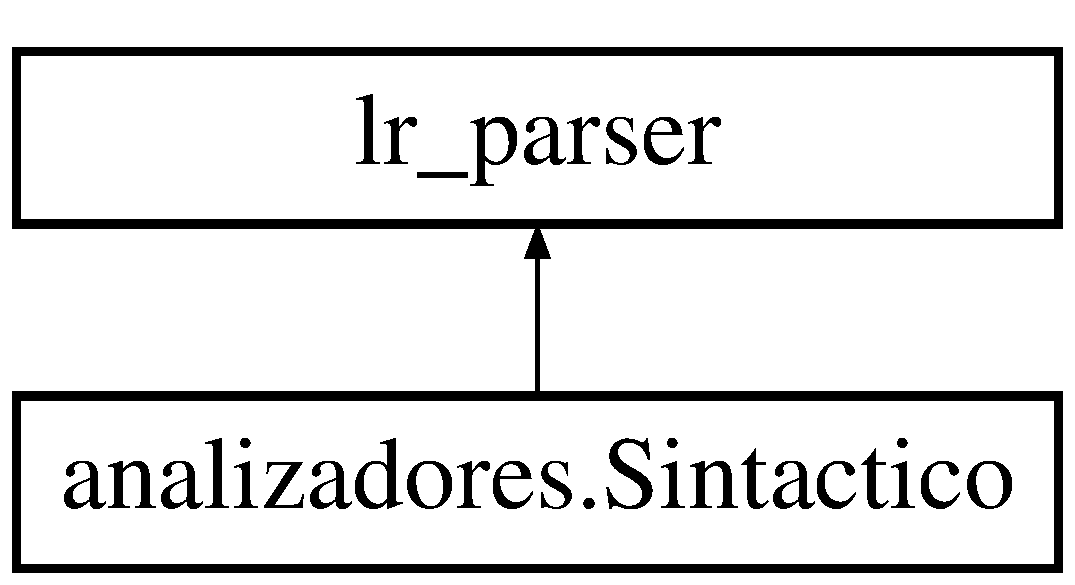
\includegraphics[height=2.000000cm]{classanalizadores_1_1_sintactico}
\end{center}
\end{figure}
\subsection*{Classes}
\begin{DoxyCompactItemize}
\item 
class {\bfseries \$actions}
\end{DoxyCompactItemize}
\subsection*{Public Member Functions}
\begin{DoxyCompactItemize}
\item 
\mbox{\Hypertarget{classanalizadores_1_1_sintactico_a671b368004366987a48baa73395922e9}\label{classanalizadores_1_1_sintactico_a671b368004366987a48baa73395922e9}} 
final Class {\bfseries get\+Symbol\+Container} ()
\item 
\mbox{\hyperlink{classanalizadores_1_1_sintactico_ab295e6867e9b03abb7a57ddafebbe17f}{Sintactico}} ()
\item 
\mbox{\hyperlink{classanalizadores_1_1_sintactico_a63738da7ca20a8b766a502b495de2d8e}{Sintactico}} (java\+\_\+cup.\+runtime.\+Scanner s)
\item 
\mbox{\hyperlink{classanalizadores_1_1_sintactico_a8c8242e3fad56503a7660fc6357e24be}{Sintactico}} (java\+\_\+cup.\+runtime.\+Scanner s, java\+\_\+cup.\+runtime.\+Symbol\+Factory sf)
\item 
short \mbox{[}$\,$\mbox{]}\mbox{[}$\,$\mbox{]} \mbox{\hyperlink{classanalizadores_1_1_sintactico_af13ccb2e45c2aa9ee26199554287de22}{production\+\_\+table}} ()
\item 
short \mbox{[}$\,$\mbox{]}\mbox{[}$\,$\mbox{]} \mbox{\hyperlink{classanalizadores_1_1_sintactico_a724ce0f5fa05d3b5d0f8e76ad5147291}{action\+\_\+table}} ()
\item 
short \mbox{[}$\,$\mbox{]}\mbox{[}$\,$\mbox{]} \mbox{\hyperlink{classanalizadores_1_1_sintactico_ab7348bf43511bec56d16c3175978e430}{reduce\+\_\+table}} ()
\item 
java\+\_\+cup.\+runtime.\+Symbol \mbox{\hyperlink{classanalizadores_1_1_sintactico_a9ea61235703a2be2386a93bda9080615}{do\+\_\+action}} (int act\+\_\+num, java\+\_\+cup.\+runtime.\+lr\+\_\+parser parser, java.\+util.\+Stack stack, int top)  throws java.\+lang.\+Exception   
\item 
int \mbox{\hyperlink{classanalizadores_1_1_sintactico_ad915f32968af0be180255e9625f3e7d9}{start\+\_\+state}} ()
\item 
int \mbox{\hyperlink{classanalizadores_1_1_sintactico_aaef47009be0140b095a5f5a0a870cf7e}{start\+\_\+production}} ()
\item 
int \mbox{\hyperlink{classanalizadores_1_1_sintactico_a7a83735fb9a0ab07d70ada5f59a38be3}{E\+O\+F\+\_\+sym}} ()
\item 
int \mbox{\hyperlink{classanalizadores_1_1_sintactico_a37c5e2a2d218a76d6126a744e30808ac}{error\+\_\+sym}} ()
\item 
void \mbox{\hyperlink{classanalizadores_1_1_sintactico_a56ace143dc3b8419ad93e4f49e43bbf4}{syntax\+\_\+error}} (Symbol s)
\item 
void \mbox{\hyperlink{classanalizadores_1_1_sintactico_a46581bb7792311a4a08c08649fe185ce}{unrecovered\+\_\+syntax\+\_\+error}} (Symbol s)  throws java.\+lang.\+Exception
\end{DoxyCompactItemize}
\subsection*{Static Public Attributes}
\begin{DoxyCompactItemize}
\item 
\mbox{\Hypertarget{classanalizadores_1_1_sintactico_ab89b63ffa29f7540b052d3b280410b1a}\label{classanalizadores_1_1_sintactico_ab89b63ffa29f7540b052d3b280410b1a}} 
static \mbox{\hyperlink{classast_1_1_a_s_t}{A\+ST}} {\bfseries arbol}
\end{DoxyCompactItemize}
\subsection*{Protected Member Functions}
\begin{DoxyCompactItemize}
\item 
void \mbox{\hyperlink{classanalizadores_1_1_sintactico_a597096a94b0afea4458c5ed107e94fa4}{init\+\_\+actions}} ()
\end{DoxyCompactItemize}
\subsection*{Protected Attributes}
\begin{DoxyCompactItemize}
\item 
C\+UP \$\mbox{\hyperlink{classanalizadores_1_1_sintactico}{Sintactico}} \$actions \mbox{\hyperlink{classanalizadores_1_1_sintactico_a7e14d36a24d6ed982b06e2b9ac181c4f}{action\+\_\+obj}}
\end{DoxyCompactItemize}
\subsection*{Static Protected Attributes}
\begin{DoxyCompactItemize}
\item 
static final short \mbox{\hyperlink{classanalizadores_1_1_sintactico_a52126500456048c148f0500de4ae22c2}{\+\_\+production\+\_\+table}} \mbox{[}$\,$\mbox{]}\mbox{[}$\,$\mbox{]}
\item 
static final short \mbox{[}$\,$\mbox{]}\mbox{[}$\,$\mbox{]} \mbox{\hyperlink{classanalizadores_1_1_sintactico_aa0bda09b109ddbd0c36c756531879b0f}{\+\_\+action\+\_\+table}}
\item 
static final short \mbox{[}$\,$\mbox{]}\mbox{[}$\,$\mbox{]} \mbox{\hyperlink{classanalizadores_1_1_sintactico_a96c2098df27363aea8d9d18a9c4fa469}{\+\_\+reduce\+\_\+table}}
\end{DoxyCompactItemize}


\subsection{Detailed Description}
C\+UP v0.\+11b 20160615 (G\+IT 4ac7450) generated parser. 

\subsection{Constructor \& Destructor Documentation}
\mbox{\Hypertarget{classanalizadores_1_1_sintactico_ab295e6867e9b03abb7a57ddafebbe17f}\label{classanalizadores_1_1_sintactico_ab295e6867e9b03abb7a57ddafebbe17f}} 
\index{analizadores\+::\+Sintactico@{analizadores\+::\+Sintactico}!Sintactico@{Sintactico}}
\index{Sintactico@{Sintactico}!analizadores\+::\+Sintactico@{analizadores\+::\+Sintactico}}
\subsubsection{\texorpdfstring{Sintactico()}{Sintactico()}\hspace{0.1cm}{\footnotesize\ttfamily [1/3]}}
{\footnotesize\ttfamily analizadores.\+Sintactico.\+Sintactico (\begin{DoxyParamCaption}{ }\end{DoxyParamCaption})}

Default constructor. \mbox{\Hypertarget{classanalizadores_1_1_sintactico_a63738da7ca20a8b766a502b495de2d8e}\label{classanalizadores_1_1_sintactico_a63738da7ca20a8b766a502b495de2d8e}} 
\index{analizadores\+::\+Sintactico@{analizadores\+::\+Sintactico}!Sintactico@{Sintactico}}
\index{Sintactico@{Sintactico}!analizadores\+::\+Sintactico@{analizadores\+::\+Sintactico}}
\subsubsection{\texorpdfstring{Sintactico()}{Sintactico()}\hspace{0.1cm}{\footnotesize\ttfamily [2/3]}}
{\footnotesize\ttfamily analizadores.\+Sintactico.\+Sintactico (\begin{DoxyParamCaption}\item[{java\+\_\+cup.\+runtime.\+Scanner}]{s }\end{DoxyParamCaption})}

Constructor which sets the default scanner. \mbox{\Hypertarget{classanalizadores_1_1_sintactico_a8c8242e3fad56503a7660fc6357e24be}\label{classanalizadores_1_1_sintactico_a8c8242e3fad56503a7660fc6357e24be}} 
\index{analizadores\+::\+Sintactico@{analizadores\+::\+Sintactico}!Sintactico@{Sintactico}}
\index{Sintactico@{Sintactico}!analizadores\+::\+Sintactico@{analizadores\+::\+Sintactico}}
\subsubsection{\texorpdfstring{Sintactico()}{Sintactico()}\hspace{0.1cm}{\footnotesize\ttfamily [3/3]}}
{\footnotesize\ttfamily analizadores.\+Sintactico.\+Sintactico (\begin{DoxyParamCaption}\item[{java\+\_\+cup.\+runtime.\+Scanner}]{s,  }\item[{java\+\_\+cup.\+runtime.\+Symbol\+Factory}]{sf }\end{DoxyParamCaption})}

Constructor which sets the default scanner. 

\subsection{Member Function Documentation}
\mbox{\Hypertarget{classanalizadores_1_1_sintactico_a724ce0f5fa05d3b5d0f8e76ad5147291}\label{classanalizadores_1_1_sintactico_a724ce0f5fa05d3b5d0f8e76ad5147291}} 
\index{analizadores\+::\+Sintactico@{analizadores\+::\+Sintactico}!action\+\_\+table@{action\+\_\+table}}
\index{action\+\_\+table@{action\+\_\+table}!analizadores\+::\+Sintactico@{analizadores\+::\+Sintactico}}
\subsubsection{\texorpdfstring{action\+\_\+table()}{action\_table()}}
{\footnotesize\ttfamily short \mbox{[}$\,$\mbox{]}\mbox{[}$\,$\mbox{]} analizadores.\+Sintactico.\+action\+\_\+table (\begin{DoxyParamCaption}{ }\end{DoxyParamCaption})}

Access to parse-\/action table. \mbox{\Hypertarget{classanalizadores_1_1_sintactico_a9ea61235703a2be2386a93bda9080615}\label{classanalizadores_1_1_sintactico_a9ea61235703a2be2386a93bda9080615}} 
\index{analizadores\+::\+Sintactico@{analizadores\+::\+Sintactico}!do\+\_\+action@{do\+\_\+action}}
\index{do\+\_\+action@{do\+\_\+action}!analizadores\+::\+Sintactico@{analizadores\+::\+Sintactico}}
\subsubsection{\texorpdfstring{do\+\_\+action()}{do\_action()}}
{\footnotesize\ttfamily java\+\_\+cup.\+runtime.\+Symbol analizadores.\+Sintactico.\+do\+\_\+action (\begin{DoxyParamCaption}\item[{int}]{act\+\_\+num,  }\item[{java\+\_\+cup.\+runtime.\+lr\+\_\+parser}]{parser,  }\item[{java.\+util.\+Stack}]{stack,  }\item[{int}]{top }\end{DoxyParamCaption}) throws java.\+lang.\+Exception}

Invoke a user supplied parse action. \mbox{\Hypertarget{classanalizadores_1_1_sintactico_a7a83735fb9a0ab07d70ada5f59a38be3}\label{classanalizadores_1_1_sintactico_a7a83735fb9a0ab07d70ada5f59a38be3}} 
\index{analizadores\+::\+Sintactico@{analizadores\+::\+Sintactico}!E\+O\+F\+\_\+sym@{E\+O\+F\+\_\+sym}}
\index{E\+O\+F\+\_\+sym@{E\+O\+F\+\_\+sym}!analizadores\+::\+Sintactico@{analizadores\+::\+Sintactico}}
\subsubsection{\texorpdfstring{E\+O\+F\+\_\+sym()}{EOF\_sym()}}
{\footnotesize\ttfamily int analizadores.\+Sintactico.\+E\+O\+F\+\_\+sym (\begin{DoxyParamCaption}{ }\end{DoxyParamCaption})}

{\ttfamily E\+OF} Symbol index. \mbox{\Hypertarget{classanalizadores_1_1_sintactico_a37c5e2a2d218a76d6126a744e30808ac}\label{classanalizadores_1_1_sintactico_a37c5e2a2d218a76d6126a744e30808ac}} 
\index{analizadores\+::\+Sintactico@{analizadores\+::\+Sintactico}!error\+\_\+sym@{error\+\_\+sym}}
\index{error\+\_\+sym@{error\+\_\+sym}!analizadores\+::\+Sintactico@{analizadores\+::\+Sintactico}}
\subsubsection{\texorpdfstring{error\+\_\+sym()}{error\_sym()}}
{\footnotesize\ttfamily int analizadores.\+Sintactico.\+error\+\_\+sym (\begin{DoxyParamCaption}{ }\end{DoxyParamCaption})}

{\ttfamily error} Symbol index. \mbox{\Hypertarget{classanalizadores_1_1_sintactico_a597096a94b0afea4458c5ed107e94fa4}\label{classanalizadores_1_1_sintactico_a597096a94b0afea4458c5ed107e94fa4}} 
\index{analizadores\+::\+Sintactico@{analizadores\+::\+Sintactico}!init\+\_\+actions@{init\+\_\+actions}}
\index{init\+\_\+actions@{init\+\_\+actions}!analizadores\+::\+Sintactico@{analizadores\+::\+Sintactico}}
\subsubsection{\texorpdfstring{init\+\_\+actions()}{init\_actions()}}
{\footnotesize\ttfamily void analizadores.\+Sintactico.\+init\+\_\+actions (\begin{DoxyParamCaption}{ }\end{DoxyParamCaption})\hspace{0.3cm}{\ttfamily [protected]}}

Action encapsulation object initializer. \mbox{\Hypertarget{classanalizadores_1_1_sintactico_af13ccb2e45c2aa9ee26199554287de22}\label{classanalizadores_1_1_sintactico_af13ccb2e45c2aa9ee26199554287de22}} 
\index{analizadores\+::\+Sintactico@{analizadores\+::\+Sintactico}!production\+\_\+table@{production\+\_\+table}}
\index{production\+\_\+table@{production\+\_\+table}!analizadores\+::\+Sintactico@{analizadores\+::\+Sintactico}}
\subsubsection{\texorpdfstring{production\+\_\+table()}{production\_table()}}
{\footnotesize\ttfamily short \mbox{[}$\,$\mbox{]}\mbox{[}$\,$\mbox{]} analizadores.\+Sintactico.\+production\+\_\+table (\begin{DoxyParamCaption}{ }\end{DoxyParamCaption})}

Access to production table. \mbox{\Hypertarget{classanalizadores_1_1_sintactico_ab7348bf43511bec56d16c3175978e430}\label{classanalizadores_1_1_sintactico_ab7348bf43511bec56d16c3175978e430}} 
\index{analizadores\+::\+Sintactico@{analizadores\+::\+Sintactico}!reduce\+\_\+table@{reduce\+\_\+table}}
\index{reduce\+\_\+table@{reduce\+\_\+table}!analizadores\+::\+Sintactico@{analizadores\+::\+Sintactico}}
\subsubsection{\texorpdfstring{reduce\+\_\+table()}{reduce\_table()}}
{\footnotesize\ttfamily short \mbox{[}$\,$\mbox{]}\mbox{[}$\,$\mbox{]} analizadores.\+Sintactico.\+reduce\+\_\+table (\begin{DoxyParamCaption}{ }\end{DoxyParamCaption})}

Access to {\ttfamily reduce\+\_\+goto} table. \mbox{\Hypertarget{classanalizadores_1_1_sintactico_aaef47009be0140b095a5f5a0a870cf7e}\label{classanalizadores_1_1_sintactico_aaef47009be0140b095a5f5a0a870cf7e}} 
\index{analizadores\+::\+Sintactico@{analizadores\+::\+Sintactico}!start\+\_\+production@{start\+\_\+production}}
\index{start\+\_\+production@{start\+\_\+production}!analizadores\+::\+Sintactico@{analizadores\+::\+Sintactico}}
\subsubsection{\texorpdfstring{start\+\_\+production()}{start\_production()}}
{\footnotesize\ttfamily int analizadores.\+Sintactico.\+start\+\_\+production (\begin{DoxyParamCaption}{ }\end{DoxyParamCaption})}

Indicates start production. \mbox{\Hypertarget{classanalizadores_1_1_sintactico_ad915f32968af0be180255e9625f3e7d9}\label{classanalizadores_1_1_sintactico_ad915f32968af0be180255e9625f3e7d9}} 
\index{analizadores\+::\+Sintactico@{analizadores\+::\+Sintactico}!start\+\_\+state@{start\+\_\+state}}
\index{start\+\_\+state@{start\+\_\+state}!analizadores\+::\+Sintactico@{analizadores\+::\+Sintactico}}
\subsubsection{\texorpdfstring{start\+\_\+state()}{start\_state()}}
{\footnotesize\ttfamily int analizadores.\+Sintactico.\+start\+\_\+state (\begin{DoxyParamCaption}{ }\end{DoxyParamCaption})}

Indicates start state. \mbox{\Hypertarget{classanalizadores_1_1_sintactico_a56ace143dc3b8419ad93e4f49e43bbf4}\label{classanalizadores_1_1_sintactico_a56ace143dc3b8419ad93e4f49e43bbf4}} 
\index{analizadores\+::\+Sintactico@{analizadores\+::\+Sintactico}!syntax\+\_\+error@{syntax\+\_\+error}}
\index{syntax\+\_\+error@{syntax\+\_\+error}!analizadores\+::\+Sintactico@{analizadores\+::\+Sintactico}}
\subsubsection{\texorpdfstring{syntax\+\_\+error()}{syntax\_error()}}
{\footnotesize\ttfamily void analizadores.\+Sintactico.\+syntax\+\_\+error (\begin{DoxyParamCaption}\item[{Symbol}]{s }\end{DoxyParamCaption})}

Método al que se llama automáticamente ante algún error sintactico. \mbox{\Hypertarget{classanalizadores_1_1_sintactico_a46581bb7792311a4a08c08649fe185ce}\label{classanalizadores_1_1_sintactico_a46581bb7792311a4a08c08649fe185ce}} 
\index{analizadores\+::\+Sintactico@{analizadores\+::\+Sintactico}!unrecovered\+\_\+syntax\+\_\+error@{unrecovered\+\_\+syntax\+\_\+error}}
\index{unrecovered\+\_\+syntax\+\_\+error@{unrecovered\+\_\+syntax\+\_\+error}!analizadores\+::\+Sintactico@{analizadores\+::\+Sintactico}}
\subsubsection{\texorpdfstring{unrecovered\+\_\+syntax\+\_\+error()}{unrecovered\_syntax\_error()}}
{\footnotesize\ttfamily void analizadores.\+Sintactico.\+unrecovered\+\_\+syntax\+\_\+error (\begin{DoxyParamCaption}\item[{Symbol}]{s }\end{DoxyParamCaption}) throws java.\+lang.\+Exception}

Método al que se llama automáticamente ante algún error sintáctico en el que ya no es posible una recuperación de errores. 

\subsection{Member Data Documentation}
\mbox{\Hypertarget{classanalizadores_1_1_sintactico_aa0bda09b109ddbd0c36c756531879b0f}\label{classanalizadores_1_1_sintactico_aa0bda09b109ddbd0c36c756531879b0f}} 
\index{analizadores\+::\+Sintactico@{analizadores\+::\+Sintactico}!\+\_\+action\+\_\+table@{\+\_\+action\+\_\+table}}
\index{\+\_\+action\+\_\+table@{\+\_\+action\+\_\+table}!analizadores\+::\+Sintactico@{analizadores\+::\+Sintactico}}
\subsubsection{\texorpdfstring{\+\_\+action\+\_\+table}{\_action\_table}}
{\footnotesize\ttfamily final short \mbox{[}$\,$\mbox{]}\mbox{[}$\,$\mbox{]} analizadores.\+Sintactico.\+\_\+action\+\_\+table\hspace{0.3cm}{\ttfamily [static]}, {\ttfamily [protected]}}

Parse-\/action table. \mbox{\Hypertarget{classanalizadores_1_1_sintactico_a52126500456048c148f0500de4ae22c2}\label{classanalizadores_1_1_sintactico_a52126500456048c148f0500de4ae22c2}} 
\index{analizadores\+::\+Sintactico@{analizadores\+::\+Sintactico}!\+\_\+production\+\_\+table@{\+\_\+production\+\_\+table}}
\index{\+\_\+production\+\_\+table@{\+\_\+production\+\_\+table}!analizadores\+::\+Sintactico@{analizadores\+::\+Sintactico}}
\subsubsection{\texorpdfstring{\+\_\+production\+\_\+table}{\_production\_table}}
{\footnotesize\ttfamily final short analizadores.\+Sintactico.\+\_\+production\+\_\+table\mbox{[}$\,$\mbox{]}\mbox{[}$\,$\mbox{]}\hspace{0.3cm}{\ttfamily [static]}, {\ttfamily [protected]}}

{\bfseries Initial value\+:}
\begin{DoxyCode}
= 
    unpackFromStrings(\textcolor{keyword}{new} String[] \{
    \textcolor{stringliteral}{"\(\backslash\)000\(\backslash\)125\(\backslash\)000\(\backslash\)002\(\backslash\)002\(\backslash\)004\(\backslash\)000\(\backslash\)002\(\backslash\)003\(\backslash\)003\(\backslash\)000\(\backslash\)002\(\backslash\)002"} +
    \textcolor{stringliteral}{"\(\backslash\)003\(\backslash\)000\(\backslash\)002\(\backslash\)004\(\backslash\)004\(\backslash\)000\(\backslash\)002\(\backslash\)004\(\backslash\)003\(\backslash\)000\(\backslash\)002\(\backslash\)006\(\backslash\)005"} +
    \textcolor{stringliteral}{"\(\backslash\)000\(\backslash\)002\(\backslash\)006\(\backslash\)004\(\backslash\)000\(\backslash\)002\(\backslash\)016\(\backslash\)011\(\backslash\)000\(\backslash\)002\(\backslash\)016\(\backslash\)010\(\backslash\)000"} +
    \textcolor{stringliteral}{"\(\backslash\)002\(\backslash\)024\(\backslash\)005\(\backslash\)000\(\backslash\)002\(\backslash\)024\(\backslash\)003\(\backslash\)000\(\backslash\)002\(\backslash\)025\(\backslash\)003\(\backslash\)000\(\backslash\)002"} +
    \textcolor{stringliteral}{"\(\backslash\)025\(\backslash\)005\(\backslash\)000\(\backslash\)002\(\backslash\)020\(\backslash\)005\(\backslash\)000\(\backslash\)002\(\backslash\)020\(\backslash\)010\(\backslash\)000\(\backslash\)002\(\backslash\)020"} +
    \textcolor{stringliteral}{"\(\backslash\)006\(\backslash\)000\(\backslash\)002\(\backslash\)020\(\backslash\)006\(\backslash\)000\(\backslash\)002\(\backslash\)020\(\backslash\)011\(\backslash\)000\(\backslash\)002\(\backslash\)020\(\backslash\)007"} +
    \textcolor{stringliteral}{"\(\backslash\)000\(\backslash\)002\(\backslash\)022\(\backslash\)004\(\backslash\)000\(\backslash\)002\(\backslash\)022\(\backslash\)003\(\backslash\)000\(\backslash\)002\(\backslash\)023\(\backslash\)005\(\backslash\)000"} +
    \textcolor{stringliteral}{"\(\backslash\)002\(\backslash\)023\(\backslash\)007\(\backslash\)000\(\backslash\)002\(\backslash\)023\(\backslash\)007\(\backslash\)000\(\backslash\)002\(\backslash\)023\(\backslash\)006\(\backslash\)000\(\backslash\)002"} +
    \textcolor{stringliteral}{"\(\backslash\)023\(\backslash\)006\(\backslash\)000\(\backslash\)002\(\backslash\)005\(\backslash\)003\(\backslash\)000\(\backslash\)002\(\backslash\)005\(\backslash\)003\(\backslash\)000\(\backslash\)002\(\backslash\)005"} +
    \textcolor{stringliteral}{"\(\backslash\)003\(\backslash\)000\(\backslash\)002\(\backslash\)005\(\backslash\)003\(\backslash\)000\(\backslash\)002\(\backslash\)005\(\backslash\)003\(\backslash\)000\(\backslash\)002\(\backslash\)005\(\backslash\)003"} +
    \textcolor{stringliteral}{"\(\backslash\)000\(\backslash\)002\(\backslash\)005\(\backslash\)003\(\backslash\)000\(\backslash\)002\(\backslash\)005\(\backslash\)003\(\backslash\)000\(\backslash\)002\(\backslash\)005\(\backslash\)003\(\backslash\)000"} +
    \textcolor{stringliteral}{"\(\backslash\)002\(\backslash\)005\(\backslash\)003\(\backslash\)000\(\backslash\)002\(\backslash\)005\(\backslash\)004\(\backslash\)000\(\backslash\)002\(\backslash\)005\(\backslash\)004\(\backslash\)000\(\backslash\)002"} +
    \textcolor{stringliteral}{"\(\backslash\)005\(\backslash\)004\(\backslash\)000\(\backslash\)002\(\backslash\)005\(\backslash\)004\(\backslash\)000\(\backslash\)002\(\backslash\)005\(\backslash\)004\(\backslash\)000\(\backslash\)002\(\backslash\)005"} +
    \textcolor{stringliteral}{"\(\backslash\)003\(\backslash\)000\(\backslash\)002\(\backslash\)021\(\backslash\)005\(\backslash\)000\(\backslash\)002\(\backslash\)021\(\backslash\)006\(\backslash\)000\(\backslash\)002\(\backslash\)007\(\backslash\)007"} +
    \textcolor{stringliteral}{"\(\backslash\)000\(\backslash\)002\(\backslash\)007\(\backslash\)011\(\backslash\)000\(\backslash\)002\(\backslash\)007\(\backslash\)011\(\backslash\)000\(\backslash\)002\(\backslash\)010\(\backslash\)007\(\backslash\)000"} +
    \textcolor{stringliteral}{"\(\backslash\)002\(\backslash\)012\(\backslash\)011\(\backslash\)000\(\backslash\)002\(\backslash\)011\(\backslash\)010\(\backslash\)000\(\backslash\)002\(\backslash\)013\(\backslash\)006\(\backslash\)000\(\backslash\)002"} +
    \textcolor{stringliteral}{"\(\backslash\)013\(\backslash\)003\(\backslash\)000\(\backslash\)002\(\backslash\)014\(\backslash\)005\(\backslash\)000\(\backslash\)002\(\backslash\)014\(\backslash\)003\(\backslash\)000\(\backslash\)002\(\backslash\)017"} +
    \textcolor{stringliteral}{"\(\backslash\)005\(\backslash\)000\(\backslash\)002\(\backslash\)017\(\backslash\)003\(\backslash\)000\(\backslash\)002\(\backslash\)015\(\backslash\)004\(\backslash\)000\(\backslash\)002\(\backslash\)015\(\backslash\)005"} +
    \textcolor{stringliteral}{"\(\backslash\)000\(\backslash\)002\(\backslash\)015\(\backslash\)005\(\backslash\)000\(\backslash\)002\(\backslash\)015\(\backslash\)005\(\backslash\)000\(\backslash\)002\(\backslash\)015\(\backslash\)005\(\backslash\)000"} +
    \textcolor{stringliteral}{"\(\backslash\)002\(\backslash\)015\(\backslash\)005\(\backslash\)000\(\backslash\)002\(\backslash\)015\(\backslash\)005\(\backslash\)000\(\backslash\)002\(\backslash\)015\(\backslash\)005\(\backslash\)000\(\backslash\)002"} +
    \textcolor{stringliteral}{"\(\backslash\)015\(\backslash\)005\(\backslash\)000\(\backslash\)002\(\backslash\)015\(\backslash\)005\(\backslash\)000\(\backslash\)002\(\backslash\)015\(\backslash\)005\(\backslash\)000\(\backslash\)002\(\backslash\)015"} +
    \textcolor{stringliteral}{"\(\backslash\)005\(\backslash\)000\(\backslash\)002\(\backslash\)015\(\backslash\)005\(\backslash\)000\(\backslash\)002\(\backslash\)015\(\backslash\)005\(\backslash\)000\(\backslash\)002\(\backslash\)015\(\backslash\)005"} +
    \textcolor{stringliteral}{"\(\backslash\)000\(\backslash\)002\(\backslash\)015\(\backslash\)004\(\backslash\)000\(\backslash\)002\(\backslash\)015\(\backslash\)007\(\backslash\)000\(\backslash\)002\(\backslash\)015\(\backslash\)005\(\backslash\)000"} +
    \textcolor{stringliteral}{"\(\backslash\)002\(\backslash\)015\(\backslash\)005\(\backslash\)000\(\backslash\)002\(\backslash\)015\(\backslash\)006\(\backslash\)000\(\backslash\)002\(\backslash\)015\(\backslash\)003\(\backslash\)000\(\backslash\)002"} +
    \textcolor{stringliteral}{"\(\backslash\)015\(\backslash\)004\(\backslash\)000\(\backslash\)002\(\backslash\)015\(\backslash\)003\(\backslash\)000\(\backslash\)002\(\backslash\)015\(\backslash\)003\(\backslash\)000\(\backslash\)002\(\backslash\)015"} +
    \textcolor{stringliteral}{"\(\backslash\)003\(\backslash\)000\(\backslash\)002\(\backslash\)015\(\backslash\)003\(\backslash\)000\(\backslash\)002\(\backslash\)015\(\backslash\)003\(\backslash\)000\(\backslash\)002\(\backslash\)015\(\backslash\)003"} +
    \textcolor{stringliteral}{"\(\backslash\)000\(\backslash\)002\(\backslash\)015\(\backslash\)003"} \})
\end{DoxyCode}
Production table. \mbox{\Hypertarget{classanalizadores_1_1_sintactico_a96c2098df27363aea8d9d18a9c4fa469}\label{classanalizadores_1_1_sintactico_a96c2098df27363aea8d9d18a9c4fa469}} 
\index{analizadores\+::\+Sintactico@{analizadores\+::\+Sintactico}!\+\_\+reduce\+\_\+table@{\+\_\+reduce\+\_\+table}}
\index{\+\_\+reduce\+\_\+table@{\+\_\+reduce\+\_\+table}!analizadores\+::\+Sintactico@{analizadores\+::\+Sintactico}}
\subsubsection{\texorpdfstring{\+\_\+reduce\+\_\+table}{\_reduce\_table}}
{\footnotesize\ttfamily final short \mbox{[}$\,$\mbox{]}\mbox{[}$\,$\mbox{]} analizadores.\+Sintactico.\+\_\+reduce\+\_\+table\hspace{0.3cm}{\ttfamily [static]}, {\ttfamily [protected]}}

{\ttfamily reduce\+\_\+goto} table. \mbox{\Hypertarget{classanalizadores_1_1_sintactico_a7e14d36a24d6ed982b06e2b9ac181c4f}\label{classanalizadores_1_1_sintactico_a7e14d36a24d6ed982b06e2b9ac181c4f}} 
\index{analizadores\+::\+Sintactico@{analizadores\+::\+Sintactico}!action\+\_\+obj@{action\+\_\+obj}}
\index{action\+\_\+obj@{action\+\_\+obj}!analizadores\+::\+Sintactico@{analizadores\+::\+Sintactico}}
\subsubsection{\texorpdfstring{action\+\_\+obj}{action\_obj}}
{\footnotesize\ttfamily C\+UP \$\mbox{\hyperlink{classanalizadores_1_1_sintactico}{Sintactico}} \$actions analizadores.\+Sintactico.\+action\+\_\+obj\hspace{0.3cm}{\ttfamily [protected]}}

Instance of action encapsulation class. 

The documentation for this class was generated from the following file\+:\begin{DoxyCompactItemize}
\item 
src/analizadores/Sintactico.\+java\end{DoxyCompactItemize}

\hypertarget{classanalizadores_1_1sym}{}\section{analizadores.\+sym Class Reference}
\label{classanalizadores_1_1sym}\index{analizadores.\+sym@{analizadores.\+sym}}
\subsection*{Static Public Attributes}
\begin{DoxyCompactItemize}
\item 
\mbox{\Hypertarget{classanalizadores_1_1sym_a2e55948a10e058c6a12f3aac3fc945a5}\label{classanalizadores_1_1sym_a2e55948a10e058c6a12f3aac3fc945a5}} 
static final int {\bfseries Twhile} = 37
\item 
\mbox{\Hypertarget{classanalizadores_1_1sym_a5c4cd575e5e50f7ff2fcaf6ed368e7f6}\label{classanalizadores_1_1sym_a5c4cd575e5e50f7ff2fcaf6ed368e7f6}} 
static final int {\bfseries P\+OR} = 12
\item 
\mbox{\Hypertarget{classanalizadores_1_1sym_a68921c7e01dba04fa23e565b43c36c23}\label{classanalizadores_1_1sym_a68921c7e01dba04fa23e565b43c36c23}} 
static final int {\bfseries Treturn} = 43
\item 
\mbox{\Hypertarget{classanalizadores_1_1sym_a96b7ec42662140f7a897a35542cb3da9}\label{classanalizadores_1_1sym_a96b7ec42662140f7a897a35542cb3da9}} 
static final int {\bfseries E\+N\+T\+E\+RO} = 45
\item 
\mbox{\Hypertarget{classanalizadores_1_1sym_a73b8707a8201c36982a84acc212dd4d0}\label{classanalizadores_1_1sym_a73b8707a8201c36982a84acc212dd4d0}} 
static final int {\bfseries D\+I\+F\+E\+R\+E\+N\+TE} = 17
\item 
\mbox{\Hypertarget{classanalizadores_1_1sym_a9322d9fdb5ed49fa3f44b4d747db07f2}\label{classanalizadores_1_1sym_a9322d9fdb5ed49fa3f44b4d747db07f2}} 
static final int {\bfseries Tfuntion} = 42
\item 
\mbox{\Hypertarget{classanalizadores_1_1sym_a7a2f729d00cf193d2a80789183cd2167}\label{classanalizadores_1_1sym_a7a2f729d00cf193d2a80789183cd2167}} 
static final int {\bfseries igual} = 25
\item 
\mbox{\Hypertarget{classanalizadores_1_1sym_a43fc8830ada2c457658ccf3d67c857d4}\label{classanalizadores_1_1sym_a43fc8830ada2c457658ccf3d67c857d4}} 
static final int {\bfseries Tnull} = 28
\item 
\mbox{\Hypertarget{classanalizadores_1_1sym_a5a72fe14fb56172391bfc2843764e648}\label{classanalizadores_1_1sym_a5a72fe14fb56172391bfc2843764e648}} 
static final int {\bfseries Tfor} = 39
\item 
\mbox{\Hypertarget{classanalizadores_1_1sym_ae3e1708165d620e42f71b53dad663b82}\label{classanalizadores_1_1sym_ae3e1708165d620e42f71b53dad663b82}} 
static final int {\bfseries ternario} = 26
\item 
\mbox{\Hypertarget{classanalizadores_1_1sym_adb8307a963f6834564e12cf28d5bd941}\label{classanalizadores_1_1sym_adb8307a963f6834564e12cf28d5bd941}} 
static final int {\bfseries Tswitch} = 36
\item 
\mbox{\Hypertarget{classanalizadores_1_1sym_ae564f10f4e52a3e0b2a53b85b94586f3}\label{classanalizadores_1_1sym_ae564f10f4e52a3e0b2a53b85b94586f3}} 
static final int {\bfseries Tnot} = 24
\item 
\mbox{\Hypertarget{classanalizadores_1_1sym_a76313b713faddd24cda698b67119f157}\label{classanalizadores_1_1sym_a76313b713faddd24cda698b67119f157}} 
static final int {\bfseries Tand} = 23
\item 
\mbox{\Hypertarget{classanalizadores_1_1sym_aba9f0c1ab038a4d9037b08a5aa1bc29a}\label{classanalizadores_1_1sym_aba9f0c1ab038a4d9037b08a5aa1bc29a}} 
static final int {\bfseries M\+E\+N\+O\+R\+I\+G\+U\+AL} = 21
\item 
\mbox{\Hypertarget{classanalizadores_1_1sym_a2a9cebdb9bf938b854b912d02899b2ad}\label{classanalizadores_1_1sym_a2a9cebdb9bf938b854b912d02899b2ad}} 
static final int {\bfseries C\+AD} = 49
\item 
\mbox{\Hypertarget{classanalizadores_1_1sym_a726f2547f9ade289d5354140b044d6f1}\label{classanalizadores_1_1sym_a726f2547f9ade289d5354140b044d6f1}} 
static final int {\bfseries tdefault} = 31
\item 
\mbox{\Hypertarget{classanalizadores_1_1sym_ab7d92b355434e62c1ee89ea230b2b63d}\label{classanalizadores_1_1sym_ab7d92b355434e62c1ee89ea230b2b63d}} 
static final int {\bfseries C\+O\+R\+D\+ER} = 6
\item 
\mbox{\Hypertarget{classanalizadores_1_1sym_a1ce46be1b560a8575260e9063a244205}\label{classanalizadores_1_1sym_a1ce46be1b560a8575260e9063a244205}} 
static final int {\bfseries D\+I\+V\+I\+D\+I\+DO} = 13
\item 
\mbox{\Hypertarget{classanalizadores_1_1sym_abb7d27ecbf14497885223c93cfa3322b}\label{classanalizadores_1_1sym_abb7d27ecbf14497885223c93cfa3322b}} 
static final int {\bfseries I\+G\+U\+A\+L\+D\+AD} = 16
\item 
\mbox{\Hypertarget{classanalizadores_1_1sym_a9f262886ec08d2b87b47b01feaeae90e}\label{classanalizadores_1_1sym_a9f262886ec08d2b87b47b01feaeae90e}} 
static final int {\bfseries Telse} = 33
\item 
\mbox{\Hypertarget{classanalizadores_1_1sym_a6d4b5cc3fbc4bdf9cb3d137a78524b62}\label{classanalizadores_1_1sym_a6d4b5cc3fbc4bdf9cb3d137a78524b62}} 
static final int {\bfseries ttrue} = 29
\item 
\mbox{\Hypertarget{classanalizadores_1_1sym_a6d95a3c17bd9fa29fca92ae2c506059e}\label{classanalizadores_1_1sym_a6d95a3c17bd9fa29fca92ae2c506059e}} 
static final int {\bfseries U\+M\+E\+N\+OS} = 47
\item 
\mbox{\Hypertarget{classanalizadores_1_1sym_a074160b81af753942e32540e148f96da}\label{classanalizadores_1_1sym_a074160b81af753942e32540e148f96da}} 
static final int {\bfseries L\+L\+A\+I\+ZQ} = 7
\item 
\mbox{\Hypertarget{classanalizadores_1_1sym_a2528f229993ba142e78bebc8ac03b64f}\label{classanalizadores_1_1sym_a2528f229993ba142e78bebc8ac03b64f}} 
static final int {\bfseries ID} = 48
\item 
\mbox{\Hypertarget{classanalizadores_1_1sym_a88e3264f7b34a6aa46ea77eaa77e77e3}\label{classanalizadores_1_1sym_a88e3264f7b34a6aa46ea77eaa77e77e3}} 
static final int {\bfseries Tdo} = 38
\item 
\mbox{\Hypertarget{classanalizadores_1_1sym_a7ac23c4c7b5a980ec4478213ed74706d}\label{classanalizadores_1_1sym_a7ac23c4c7b5a980ec4478213ed74706d}} 
static final int {\bfseries M\+A\+Y\+O\+R\+I\+G\+U\+AL} = 20
\item 
\mbox{\Hypertarget{classanalizadores_1_1sym_ae961425a5e76e27af6c32d1f170f12f9}\label{classanalizadores_1_1sym_ae961425a5e76e27af6c32d1f170f12f9}} 
static final int {\bfseries D\+E\+C\+I\+M\+AL} = 46
\item 
\mbox{\Hypertarget{classanalizadores_1_1sym_a06a51a9d046200bafd9b34732ce20ff5}\label{classanalizadores_1_1sym_a06a51a9d046200bafd9b34732ce20ff5}} 
static final int {\bfseries E\+OF} = 0
\item 
\mbox{\Hypertarget{classanalizadores_1_1sym_a7a9e530087d1c421a505813671391352}\label{classanalizadores_1_1sym_a7a9e530087d1c421a505813671391352}} 
static final int {\bfseries P\+A\+R\+I\+ZQ} = 3
\item 
\mbox{\Hypertarget{classanalizadores_1_1sym_a18da1773060a96700b2b9c282024eb36}\label{classanalizadores_1_1sym_a18da1773060a96700b2b9c282024eb36}} 
static final int {\bfseries error} = 1
\item 
\mbox{\Hypertarget{classanalizadores_1_1sym_a1f7dd2b6fd11f4545a7bb4834693eec9}\label{classanalizadores_1_1sym_a1f7dd2b6fd11f4545a7bb4834693eec9}} 
static final int {\bfseries C\+O\+MA} = 9
\item 
\mbox{\Hypertarget{classanalizadores_1_1sym_aad5704d093d7068612a6d8f0d28cb044}\label{classanalizadores_1_1sym_aad5704d093d7068612a6d8f0d28cb044}} 
static final int {\bfseries M\+O\+D\+U\+LO} = 15
\item 
\mbox{\Hypertarget{classanalizadores_1_1sym_acc834d6db6273d5a07c9d7a66f6d9590}\label{classanalizadores_1_1sym_acc834d6db6273d5a07c9d7a66f6d9590}} 
static final int {\bfseries M\+E\+N\+OS} = 11
\item 
\mbox{\Hypertarget{classanalizadores_1_1sym_a09d42021a1a6a511b2fc5a5bb3542f61}\label{classanalizadores_1_1sym_a09d42021a1a6a511b2fc5a5bb3542f61}} 
static final int {\bfseries M\+E\+N\+OR} = 19
\item 
\mbox{\Hypertarget{classanalizadores_1_1sym_afefd098a6cb8568589ed87243c0cf204}\label{classanalizadores_1_1sym_afefd098a6cb8568589ed87243c0cf204}} 
static final int {\bfseries dospuntos} = 27
\item 
\mbox{\Hypertarget{classanalizadores_1_1sym_a6b53b27a977dc9809913c0d27888b5a4}\label{classanalizadores_1_1sym_a6b53b27a977dc9809913c0d27888b5a4}} 
static final int {\bfseries M\+A\+Y\+OR} = 18
\item 
\mbox{\Hypertarget{classanalizadores_1_1sym_a6ee78ee38e63e1050918fa7d240613aa}\label{classanalizadores_1_1sym_a6ee78ee38e63e1050918fa7d240613aa}} 
static final int {\bfseries tfalse} = 30
\item 
\mbox{\Hypertarget{classanalizadores_1_1sym_ad5979ee36b37823938f29baf0ea15d7a}\label{classanalizadores_1_1sym_ad5979ee36b37823938f29baf0ea15d7a}} 
static final int {\bfseries P\+O\+T\+E\+N\+C\+IA} = 14
\item 
\mbox{\Hypertarget{classanalizadores_1_1sym_ab15c5d3e1b9c53961ba9d6546cfcb08b}\label{classanalizadores_1_1sym_ab15c5d3e1b9c53961ba9d6546cfcb08b}} 
static final int {\bfseries fantasmita} = 44
\item 
\mbox{\Hypertarget{classanalizadores_1_1sym_a138b04b55959974ceea3213ab59643a7}\label{classanalizadores_1_1sym_a138b04b55959974ceea3213ab59643a7}} 
static final int {\bfseries Tcase} = 35
\item 
\mbox{\Hypertarget{classanalizadores_1_1sym_a520de7d0900f89aff83eb51ddc2fa15f}\label{classanalizadores_1_1sym_a520de7d0900f89aff83eb51ddc2fa15f}} 
static final int {\bfseries Tin} = 40
\item 
\mbox{\Hypertarget{classanalizadores_1_1sym_a2384fa20a2c92fbe4053fb0809d8767e}\label{classanalizadores_1_1sym_a2384fa20a2c92fbe4053fb0809d8767e}} 
static final int {\bfseries P\+T\+C\+O\+MA} = 2
\item 
\mbox{\Hypertarget{classanalizadores_1_1sym_a633120b6b73f79c89c860adfaf8f8ea4}\label{classanalizadores_1_1sym_a633120b6b73f79c89c860adfaf8f8ea4}} 
static final int {\bfseries Tor} = 22
\item 
\mbox{\Hypertarget{classanalizadores_1_1sym_a47dcd33c94d410877fbcca792bc5ee54}\label{classanalizadores_1_1sym_a47dcd33c94d410877fbcca792bc5ee54}} 
static final int {\bfseries Tbreak} = 34
\item 
\mbox{\Hypertarget{classanalizadores_1_1sym_ad63abef425c2b18dda1ccb959358e704}\label{classanalizadores_1_1sym_ad63abef425c2b18dda1ccb959358e704}} 
static final int {\bfseries L\+L\+A\+D\+ER} = 8
\item 
\mbox{\Hypertarget{classanalizadores_1_1sym_a02cdf13eb2481d97b0c8f5928cc74817}\label{classanalizadores_1_1sym_a02cdf13eb2481d97b0c8f5928cc74817}} 
static final int {\bfseries P\+A\+R\+D\+ER} = 4
\item 
\mbox{\Hypertarget{classanalizadores_1_1sym_a79c3c0929cccad3c9ee7da492e3911f4}\label{classanalizadores_1_1sym_a79c3c0929cccad3c9ee7da492e3911f4}} 
static final int {\bfseries C\+O\+R\+I\+ZQ} = 5
\item 
\mbox{\Hypertarget{classanalizadores_1_1sym_a33fbdc7b9b9054bb272c591dfd7ec3b6}\label{classanalizadores_1_1sym_a33fbdc7b9b9054bb272c591dfd7ec3b6}} 
static final int {\bfseries Tif} = 32
\item 
\mbox{\Hypertarget{classanalizadores_1_1sym_a3c58f13b33bd7e1673661d9c17fb02dd}\label{classanalizadores_1_1sym_a3c58f13b33bd7e1673661d9c17fb02dd}} 
static final int {\bfseries Tcontinue} = 41
\item 
\mbox{\Hypertarget{classanalizadores_1_1sym_aff7c3629c18bbb18dbf247bdc7819712}\label{classanalizadores_1_1sym_aff7c3629c18bbb18dbf247bdc7819712}} 
static final int {\bfseries M\+AS} = 10
\item 
\mbox{\Hypertarget{classanalizadores_1_1sym_a4ed81fab67983049691d8adffd882f90}\label{classanalizadores_1_1sym_a4ed81fab67983049691d8adffd882f90}} 
static final String \mbox{[}$\,$\mbox{]} {\bfseries terminal\+Names}
\end{DoxyCompactItemize}


\subsection{Detailed Description}
C\+UP generated class containing symbol constants. 

The documentation for this class was generated from the following file\+:\begin{DoxyCompactItemize}
\item 
src/analizadores/sym.\+java\end{DoxyCompactItemize}

\hypertarget{classast_1_1expresiones_1_1operaciones_1_1_ternaria}{}\section{ast.\+expresiones.\+operaciones.\+Ternaria Class Reference}
\label{classast_1_1expresiones_1_1operaciones_1_1_ternaria}\index{ast.\+expresiones.\+operaciones.\+Ternaria@{ast.\+expresiones.\+operaciones.\+Ternaria}}
Inheritance diagram for ast.\+expresiones.\+operaciones.\+Ternaria\+:\begin{figure}[H]
\begin{center}
\leavevmode
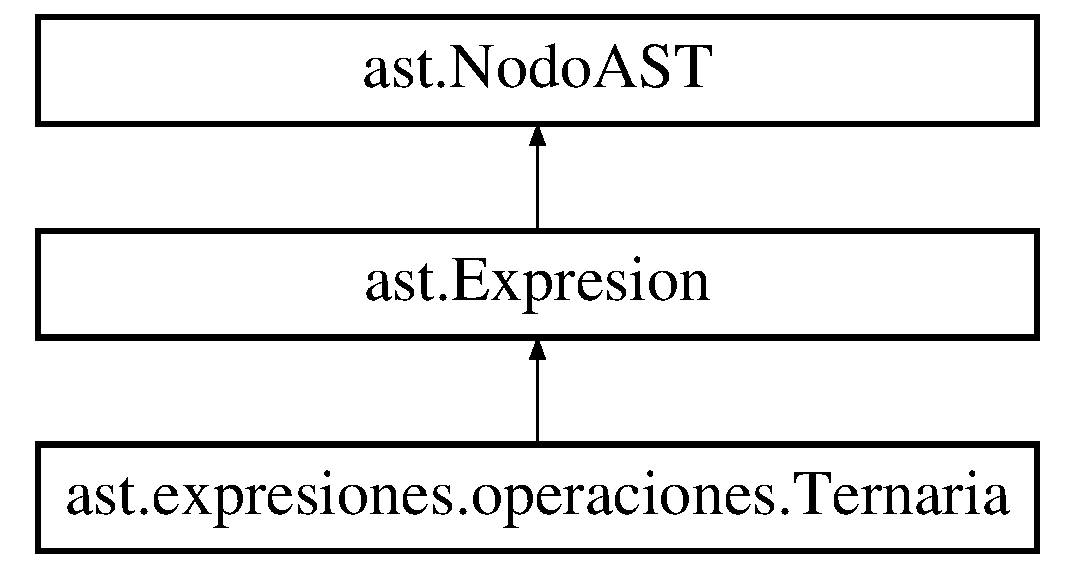
\includegraphics[height=3.000000cm]{classast_1_1expresiones_1_1operaciones_1_1_ternaria}
\end{center}
\end{figure}
\subsection*{Public Member Functions}
\begin{DoxyCompactItemize}
\item 
\mbox{\Hypertarget{classast_1_1expresiones_1_1operaciones_1_1_ternaria_a64b6ad4de626de178cb6755ecade9519}\label{classast_1_1expresiones_1_1operaciones_1_1_ternaria_a64b6ad4de626de178cb6755ecade9519}} 
{\bfseries Ternaria} (\mbox{\hyperlink{interfaceast_1_1_expresion}{Expresion}} ex1, \mbox{\hyperlink{interfaceast_1_1_expresion}{Expresion}} ex2, \mbox{\hyperlink{interfaceast_1_1_expresion}{Expresion}} ex3, int linea, int col)
\item 
\mbox{\Hypertarget{classast_1_1expresiones_1_1operaciones_1_1_ternaria_a460aa20abeeca05f8418650686bff361}\label{classast_1_1expresiones_1_1operaciones_1_1_ternaria_a460aa20abeeca05f8418650686bff361}} 
\mbox{\hyperlink{classentorno_1_1_tipo}{Tipo}} {\bfseries get\+Tipo} (\mbox{\hyperlink{classentorno_1_1_entorno}{Entorno}} ent)
\item 
\mbox{\Hypertarget{classast_1_1expresiones_1_1operaciones_1_1_ternaria_a07b689bcc58b97b837291569a740cc05}\label{classast_1_1expresiones_1_1operaciones_1_1_ternaria_a07b689bcc58b97b837291569a740cc05}} 
Object {\bfseries get\+Valor\+Implicito} (\mbox{\hyperlink{classentorno_1_1_entorno}{Entorno}} ent)
\item 
\mbox{\Hypertarget{classast_1_1expresiones_1_1operaciones_1_1_ternaria_a8dc5b11a40414296a32a550e987029f2}\label{classast_1_1expresiones_1_1operaciones_1_1_ternaria_a8dc5b11a40414296a32a550e987029f2}} 
int {\bfseries linea} ()
\item 
\mbox{\Hypertarget{classast_1_1expresiones_1_1operaciones_1_1_ternaria_adcaf20cf1bda131dad5aef6c47a0da6b}\label{classast_1_1expresiones_1_1operaciones_1_1_ternaria_adcaf20cf1bda131dad5aef6c47a0da6b}} 
int {\bfseries columna} ()
\item 
\mbox{\Hypertarget{classast_1_1expresiones_1_1operaciones_1_1_ternaria_a79bd4eed4dd4752fcdc2397861129caa}\label{classast_1_1expresiones_1_1operaciones_1_1_ternaria_a79bd4eed4dd4752fcdc2397861129caa}} 
String {\bfseries get\+Nombre} (String\+Builder builder, String parent, int cont)
\end{DoxyCompactItemize}


\subsection{Detailed Description}
\begin{DoxyAuthor}{Author}
p\+\_\+ab1 
\end{DoxyAuthor}


The documentation for this class was generated from the following file\+:\begin{DoxyCompactItemize}
\item 
src/ast/expresiones/operaciones/Ternaria.\+java\end{DoxyCompactItemize}

\hypertarget{classentorno_1_1_tipo}{}\section{entorno.\+Tipo Class Reference}
\label{classentorno_1_1_tipo}\index{entorno.\+Tipo@{entorno.\+Tipo}}
\subsection*{Classes}
\begin{DoxyCompactItemize}
\item 
enum \mbox{\hyperlink{enumentorno_1_1_tipo_1_1_tipos}{Tipos}}
\end{DoxyCompactItemize}
\subsection*{Public Member Functions}
\begin{DoxyCompactItemize}
\item 
\mbox{\Hypertarget{classentorno_1_1_tipo_a882db5acc300a944b077aee431238539}\label{classentorno_1_1_tipo_a882db5acc300a944b077aee431238539}} 
{\bfseries Tipo} (\mbox{\hyperlink{enumentorno_1_1_tipo_1_1_tipos}{Tipos}} tp)
\item 
\mbox{\Hypertarget{classentorno_1_1_tipo_a14a0af6d92ec4968334dfda133955fce}\label{classentorno_1_1_tipo_a14a0af6d92ec4968334dfda133955fce}} 
\mbox{\hyperlink{enumentorno_1_1_tipo_1_1_tipos}{Tipos}} {\bfseries get\+Tipo\+Primitivo} ()
\item 
\mbox{\Hypertarget{classentorno_1_1_tipo_a51be477d58b52e4f461683f06c8b90c8}\label{classentorno_1_1_tipo_a51be477d58b52e4f461683f06c8b90c8}} 
boolean {\bfseries is\+Numeric} ()
\item 
\mbox{\Hypertarget{classentorno_1_1_tipo_ad874eeb699751c1c9e7c0b4fcfb43fb7}\label{classentorno_1_1_tipo_ad874eeb699751c1c9e7c0b4fcfb43fb7}} 
boolean {\bfseries is\+Boolean} ()
\item 
\mbox{\Hypertarget{classentorno_1_1_tipo_ae75ea520879013495d3ae3770f04f01c}\label{classentorno_1_1_tipo_ae75ea520879013495d3ae3770f04f01c}} 
boolean {\bfseries is\+Double} ()
\item 
\mbox{\Hypertarget{classentorno_1_1_tipo_aa5258513322b2bcb8862d5c4fc760f31}\label{classentorno_1_1_tipo_aa5258513322b2bcb8862d5c4fc760f31}} 
boolean {\bfseries is\+Int} ()
\item 
\mbox{\Hypertarget{classentorno_1_1_tipo_a1284ae01f6293a1ea856ea5e5c645773}\label{classentorno_1_1_tipo_a1284ae01f6293a1ea856ea5e5c645773}} 
boolean {\bfseries is\+String} ()
\end{DoxyCompactItemize}


\subsection{Detailed Description}
\begin{DoxyAuthor}{Author}
p\+\_\+ab1 
\end{DoxyAuthor}


The documentation for this class was generated from the following file\+:\begin{DoxyCompactItemize}
\item 
src/entorno/Tipo.\+java\end{DoxyCompactItemize}

\hypertarget{enumentorno_1_1_tipo_1_1_tipos}{}\section{entorno.\+Tipo.\+Tipos Enum Reference}
\label{enumentorno_1_1_tipo_1_1_tipos}\index{entorno.\+Tipo.\+Tipos@{entorno.\+Tipo.\+Tipos}}
\subsection*{Public Attributes}
\begin{DoxyCompactItemize}
\item 
\mbox{\Hypertarget{enumentorno_1_1_tipo_1_1_tipos_a897dd5c2009e0eaf6b60f826dbc8e2a7}\label{enumentorno_1_1_tipo_1_1_tipos_a897dd5c2009e0eaf6b60f826dbc8e2a7}} 
{\bfseries S\+T\+R\+I\+NG}
\item 
\mbox{\Hypertarget{enumentorno_1_1_tipo_1_1_tipos_a5b247a6c9534e292a13e1d45cdeb3e29}\label{enumentorno_1_1_tipo_1_1_tipos_a5b247a6c9534e292a13e1d45cdeb3e29}} 
{\bfseries I\+NT}
\item 
\mbox{\Hypertarget{enumentorno_1_1_tipo_1_1_tipos_a6fde90546e91983ac63b60a154672f02}\label{enumentorno_1_1_tipo_1_1_tipos_a6fde90546e91983ac63b60a154672f02}} 
{\bfseries D\+O\+U\+B\+LE}
\item 
\mbox{\Hypertarget{enumentorno_1_1_tipo_1_1_tipos_a1872240c69e6b247d8d4ee956a8b619b}\label{enumentorno_1_1_tipo_1_1_tipos_a1872240c69e6b247d8d4ee956a8b619b}} 
{\bfseries B\+O\+OL}
\item 
\mbox{\Hypertarget{enumentorno_1_1_tipo_1_1_tipos_a8074f85e0811ec2a837f432738d781f1}\label{enumentorno_1_1_tipo_1_1_tipos_a8074f85e0811ec2a837f432738d781f1}} 
{\bfseries V\+O\+ID}
\item 
\mbox{\Hypertarget{enumentorno_1_1_tipo_1_1_tipos_a32165ce9029d548e2faa25c0c0fda301}\label{enumentorno_1_1_tipo_1_1_tipos_a32165ce9029d548e2faa25c0c0fda301}} 
{\bfseries D\+E\+F\+A\+U\+LT}
\item 
\mbox{\Hypertarget{enumentorno_1_1_tipo_1_1_tipos_ad6b959b7441f58b43dfc1dadde9c668a}\label{enumentorno_1_1_tipo_1_1_tipos_ad6b959b7441f58b43dfc1dadde9c668a}} 
{\bfseries L\+I\+ST}
\item 
\mbox{\Hypertarget{enumentorno_1_1_tipo_1_1_tipos_a298ec6b9bf944ba4ffef6d3dd2293cfc}\label{enumentorno_1_1_tipo_1_1_tipos_a298ec6b9bf944ba4ffef6d3dd2293cfc}} 
{\bfseries M\+A\+T\+R\+IZ}
\end{DoxyCompactItemize}


The documentation for this enum was generated from the following file\+:\begin{DoxyCompactItemize}
\item 
src/entorno/Tipo.\+java\end{DoxyCompactItemize}

\hypertarget{classanalizadores_1_1_token}{}\section{analizadores.\+Token Class Reference}
\label{classanalizadores_1_1_token}\index{analizadores.\+Token@{analizadores.\+Token}}
\subsection*{Public Member Functions}
\begin{DoxyCompactItemize}
\item 
Object \mbox{\hyperlink{classanalizadores_1_1_token_ac7dec28cd30fc7fe1e678d8aec55008d}{get\+Value}} ()
\item 
\mbox{\hyperlink{classanalizadores_1_1_token_afe5ae37eb50ea338fa7159207f58ace9}{Token}} ()
\item 
\mbox{\hyperlink{classanalizadores_1_1_token_aeb457a7f26dda041155527fecbc475b6}{Token}} (int \mbox{\hyperlink{classanalizadores_1_1_token_ac5615b76c325a751915025aa28a03cfc}{kind}})
\item 
\mbox{\hyperlink{classanalizadores_1_1_token_a7691eebbf98eb55d3c338cb8d7dfccd6}{Token}} (int \mbox{\hyperlink{classanalizadores_1_1_token_ac5615b76c325a751915025aa28a03cfc}{kind}}, String \mbox{\hyperlink{classanalizadores_1_1_token_a3636b082aca90dcbd24df1790f847590}{image}})
\item 
String \mbox{\hyperlink{classanalizadores_1_1_token_a6b1216eeaff66da8354424d684fe0eb2}{to\+String}} ()
\end{DoxyCompactItemize}
\subsection*{Static Public Member Functions}
\begin{DoxyCompactItemize}
\item 
static \mbox{\hyperlink{classanalizadores_1_1_token}{Token}} \mbox{\hyperlink{classanalizadores_1_1_token_aca2ccbc7bd267f4098be9f4a0b07fc47}{new\+Token}} (int of\+Kind, String \mbox{\hyperlink{classanalizadores_1_1_token_a3636b082aca90dcbd24df1790f847590}{image}})
\item 
\mbox{\Hypertarget{classanalizadores_1_1_token_ae617d54f335f4292715da074aa8a0abe}\label{classanalizadores_1_1_token_ae617d54f335f4292715da074aa8a0abe}} 
static \mbox{\hyperlink{classanalizadores_1_1_token}{Token}} {\bfseries new\+Token} (int of\+Kind)
\end{DoxyCompactItemize}
\subsection*{Public Attributes}
\begin{DoxyCompactItemize}
\item 
int \mbox{\hyperlink{classanalizadores_1_1_token_ac5615b76c325a751915025aa28a03cfc}{kind}}
\item 
int \mbox{\hyperlink{classanalizadores_1_1_token_afaec87d0c77c8f37692f7b1061e2955a}{begin\+Line}}
\item 
int \mbox{\hyperlink{classanalizadores_1_1_token_a3274d7ca281b55d20fbdfad269762456}{begin\+Column}}
\item 
int \mbox{\hyperlink{classanalizadores_1_1_token_a37afccf406a7948b763ccb503afecc4f}{end\+Line}}
\item 
int \mbox{\hyperlink{classanalizadores_1_1_token_adc8a8b5671f861de75274cb8016064b9}{end\+Column}}
\item 
String \mbox{\hyperlink{classanalizadores_1_1_token_a3636b082aca90dcbd24df1790f847590}{image}}
\item 
\mbox{\hyperlink{classanalizadores_1_1_token}{Token}} \mbox{\hyperlink{classanalizadores_1_1_token_a7177e7c2f1387bb011e8602a52077126}{next}}
\item 
\mbox{\hyperlink{classanalizadores_1_1_token}{Token}} \mbox{\hyperlink{classanalizadores_1_1_token_a05c70c5bef44be3c3126ed5c267978fd}{special\+Token}}
\end{DoxyCompactItemize}


\subsection{Detailed Description}
Describes the input token stream. 

\subsection{Constructor \& Destructor Documentation}
\mbox{\Hypertarget{classanalizadores_1_1_token_afe5ae37eb50ea338fa7159207f58ace9}\label{classanalizadores_1_1_token_afe5ae37eb50ea338fa7159207f58ace9}} 
\index{analizadores\+::\+Token@{analizadores\+::\+Token}!Token@{Token}}
\index{Token@{Token}!analizadores\+::\+Token@{analizadores\+::\+Token}}
\subsubsection{\texorpdfstring{Token()}{Token()}\hspace{0.1cm}{\footnotesize\ttfamily [1/3]}}
{\footnotesize\ttfamily analizadores.\+Token.\+Token (\begin{DoxyParamCaption}{ }\end{DoxyParamCaption})}

No-\/argument contructor \mbox{\Hypertarget{classanalizadores_1_1_token_aeb457a7f26dda041155527fecbc475b6}\label{classanalizadores_1_1_token_aeb457a7f26dda041155527fecbc475b6}} 
\index{analizadores\+::\+Token@{analizadores\+::\+Token}!Token@{Token}}
\index{Token@{Token}!analizadores\+::\+Token@{analizadores\+::\+Token}}
\subsubsection{\texorpdfstring{Token()}{Token()}\hspace{0.1cm}{\footnotesize\ttfamily [2/3]}}
{\footnotesize\ttfamily analizadores.\+Token.\+Token (\begin{DoxyParamCaption}\item[{int}]{kind }\end{DoxyParamCaption})}

Constructs a new token for the specified Image. \mbox{\Hypertarget{classanalizadores_1_1_token_a7691eebbf98eb55d3c338cb8d7dfccd6}\label{classanalizadores_1_1_token_a7691eebbf98eb55d3c338cb8d7dfccd6}} 
\index{analizadores\+::\+Token@{analizadores\+::\+Token}!Token@{Token}}
\index{Token@{Token}!analizadores\+::\+Token@{analizadores\+::\+Token}}
\subsubsection{\texorpdfstring{Token()}{Token()}\hspace{0.1cm}{\footnotesize\ttfamily [3/3]}}
{\footnotesize\ttfamily analizadores.\+Token.\+Token (\begin{DoxyParamCaption}\item[{int}]{kind,  }\item[{String}]{image }\end{DoxyParamCaption})}

Constructs a new token for the specified Image and Kind. 

\subsection{Member Function Documentation}
\mbox{\Hypertarget{classanalizadores_1_1_token_ac7dec28cd30fc7fe1e678d8aec55008d}\label{classanalizadores_1_1_token_ac7dec28cd30fc7fe1e678d8aec55008d}} 
\index{analizadores\+::\+Token@{analizadores\+::\+Token}!get\+Value@{get\+Value}}
\index{get\+Value@{get\+Value}!analizadores\+::\+Token@{analizadores\+::\+Token}}
\subsubsection{\texorpdfstring{get\+Value()}{getValue()}}
{\footnotesize\ttfamily Object analizadores.\+Token.\+get\+Value (\begin{DoxyParamCaption}{ }\end{DoxyParamCaption})}

An optional attribute value of the \mbox{\hyperlink{classanalizadores_1_1_token}{Token}}. Tokens which are not used as syntactic sugar will often contain meaningful values that will be used later on by the compiler or interpreter. This attribute value is often different from the image. Any subclass of \mbox{\hyperlink{classanalizadores_1_1_token}{Token}} that actually wants to return a non-\/null value can override this method as appropriate. \mbox{\Hypertarget{classanalizadores_1_1_token_aca2ccbc7bd267f4098be9f4a0b07fc47}\label{classanalizadores_1_1_token_aca2ccbc7bd267f4098be9f4a0b07fc47}} 
\index{analizadores\+::\+Token@{analizadores\+::\+Token}!new\+Token@{new\+Token}}
\index{new\+Token@{new\+Token}!analizadores\+::\+Token@{analizadores\+::\+Token}}
\subsubsection{\texorpdfstring{new\+Token()}{newToken()}}
{\footnotesize\ttfamily static \mbox{\hyperlink{classanalizadores_1_1_token}{Token}} analizadores.\+Token.\+new\+Token (\begin{DoxyParamCaption}\item[{int}]{of\+Kind,  }\item[{String}]{image }\end{DoxyParamCaption})\hspace{0.3cm}{\ttfamily [static]}}

Returns a new \mbox{\hyperlink{classanalizadores_1_1_token}{Token}} object, by default. However, if you want, you can create and return subclass objects based on the value of of\+Kind. Simply add the cases to the switch for all those special cases. For example, if you have a subclass of \mbox{\hyperlink{classanalizadores_1_1_token}{Token}} called I\+D\+Token that you want to create if of\+Kind is ID, simply add something like \+:

case My\+Parser\+Constants.\+ID \+: return new I\+D\+Token(of\+Kind, image);

to the following switch statement. Then you can cast matched\+Token variable to the appropriate type and use sit in your lexical actions. \mbox{\Hypertarget{classanalizadores_1_1_token_a6b1216eeaff66da8354424d684fe0eb2}\label{classanalizadores_1_1_token_a6b1216eeaff66da8354424d684fe0eb2}} 
\index{analizadores\+::\+Token@{analizadores\+::\+Token}!to\+String@{to\+String}}
\index{to\+String@{to\+String}!analizadores\+::\+Token@{analizadores\+::\+Token}}
\subsubsection{\texorpdfstring{to\+String()}{toString()}}
{\footnotesize\ttfamily String analizadores.\+Token.\+to\+String (\begin{DoxyParamCaption}{ }\end{DoxyParamCaption})}

Returns the image. 

\subsection{Member Data Documentation}
\mbox{\Hypertarget{classanalizadores_1_1_token_a3274d7ca281b55d20fbdfad269762456}\label{classanalizadores_1_1_token_a3274d7ca281b55d20fbdfad269762456}} 
\index{analizadores\+::\+Token@{analizadores\+::\+Token}!begin\+Column@{begin\+Column}}
\index{begin\+Column@{begin\+Column}!analizadores\+::\+Token@{analizadores\+::\+Token}}
\subsubsection{\texorpdfstring{begin\+Column}{beginColumn}}
{\footnotesize\ttfamily int analizadores.\+Token.\+begin\+Column}

The column number of the first character of this \mbox{\hyperlink{classanalizadores_1_1_token}{Token}}. \mbox{\Hypertarget{classanalizadores_1_1_token_afaec87d0c77c8f37692f7b1061e2955a}\label{classanalizadores_1_1_token_afaec87d0c77c8f37692f7b1061e2955a}} 
\index{analizadores\+::\+Token@{analizadores\+::\+Token}!begin\+Line@{begin\+Line}}
\index{begin\+Line@{begin\+Line}!analizadores\+::\+Token@{analizadores\+::\+Token}}
\subsubsection{\texorpdfstring{begin\+Line}{beginLine}}
{\footnotesize\ttfamily int analizadores.\+Token.\+begin\+Line}

The line number of the first character of this \mbox{\hyperlink{classanalizadores_1_1_token}{Token}}. \mbox{\Hypertarget{classanalizadores_1_1_token_adc8a8b5671f861de75274cb8016064b9}\label{classanalizadores_1_1_token_adc8a8b5671f861de75274cb8016064b9}} 
\index{analizadores\+::\+Token@{analizadores\+::\+Token}!end\+Column@{end\+Column}}
\index{end\+Column@{end\+Column}!analizadores\+::\+Token@{analizadores\+::\+Token}}
\subsubsection{\texorpdfstring{end\+Column}{endColumn}}
{\footnotesize\ttfamily int analizadores.\+Token.\+end\+Column}

The column number of the last character of this \mbox{\hyperlink{classanalizadores_1_1_token}{Token}}. \mbox{\Hypertarget{classanalizadores_1_1_token_a37afccf406a7948b763ccb503afecc4f}\label{classanalizadores_1_1_token_a37afccf406a7948b763ccb503afecc4f}} 
\index{analizadores\+::\+Token@{analizadores\+::\+Token}!end\+Line@{end\+Line}}
\index{end\+Line@{end\+Line}!analizadores\+::\+Token@{analizadores\+::\+Token}}
\subsubsection{\texorpdfstring{end\+Line}{endLine}}
{\footnotesize\ttfamily int analizadores.\+Token.\+end\+Line}

The line number of the last character of this \mbox{\hyperlink{classanalizadores_1_1_token}{Token}}. \mbox{\Hypertarget{classanalizadores_1_1_token_a3636b082aca90dcbd24df1790f847590}\label{classanalizadores_1_1_token_a3636b082aca90dcbd24df1790f847590}} 
\index{analizadores\+::\+Token@{analizadores\+::\+Token}!image@{image}}
\index{image@{image}!analizadores\+::\+Token@{analizadores\+::\+Token}}
\subsubsection{\texorpdfstring{image}{image}}
{\footnotesize\ttfamily String analizadores.\+Token.\+image}

The string image of the token. \mbox{\Hypertarget{classanalizadores_1_1_token_ac5615b76c325a751915025aa28a03cfc}\label{classanalizadores_1_1_token_ac5615b76c325a751915025aa28a03cfc}} 
\index{analizadores\+::\+Token@{analizadores\+::\+Token}!kind@{kind}}
\index{kind@{kind}!analizadores\+::\+Token@{analizadores\+::\+Token}}
\subsubsection{\texorpdfstring{kind}{kind}}
{\footnotesize\ttfamily int analizadores.\+Token.\+kind}

An integer that describes the kind of this token. This numbering system is determined by Java\+C\+C\+Parser, and a table of these numbers is stored in the file ...Constants.\+java. \mbox{\Hypertarget{classanalizadores_1_1_token_a7177e7c2f1387bb011e8602a52077126}\label{classanalizadores_1_1_token_a7177e7c2f1387bb011e8602a52077126}} 
\index{analizadores\+::\+Token@{analizadores\+::\+Token}!next@{next}}
\index{next@{next}!analizadores\+::\+Token@{analizadores\+::\+Token}}
\subsubsection{\texorpdfstring{next}{next}}
{\footnotesize\ttfamily \mbox{\hyperlink{classanalizadores_1_1_token}{Token}} analizadores.\+Token.\+next}

A reference to the next regular (non-\/special) token from the input stream. If this is the last token from the input stream, or if the token manager has not read tokens beyond this one, this field is set to null. This is true only if this token is also a regular token. Otherwise, see below for a description of the contents of this field. \mbox{\Hypertarget{classanalizadores_1_1_token_a05c70c5bef44be3c3126ed5c267978fd}\label{classanalizadores_1_1_token_a05c70c5bef44be3c3126ed5c267978fd}} 
\index{analizadores\+::\+Token@{analizadores\+::\+Token}!special\+Token@{special\+Token}}
\index{special\+Token@{special\+Token}!analizadores\+::\+Token@{analizadores\+::\+Token}}
\subsubsection{\texorpdfstring{special\+Token}{specialToken}}
{\footnotesize\ttfamily \mbox{\hyperlink{classanalizadores_1_1_token}{Token}} analizadores.\+Token.\+special\+Token}

This field is used to access special tokens that occur prior to this token, but after the immediately preceding regular (non-\/special) token. If there are no such special tokens, this field is set to null. When there are more than one such special token, this field refers to the last of these special tokens, which in turn refers to the next previous special token through its special\+Token field, and so on until the first special token (whose special\+Token field is null). The next fields of special tokens refer to other special tokens that immediately follow it (without an intervening regular token). If there is no such token, this field is null. 

The documentation for this class was generated from the following file\+:\begin{DoxyCompactItemize}
\item 
src/analizadores/Token.\+java\end{DoxyCompactItemize}

\hypertarget{classanalizadores_1_1_token_mgr_error}{}\section{analizadores.\+Token\+Mgr\+Error Class Reference}
\label{classanalizadores_1_1_token_mgr_error}\index{analizadores.\+Token\+Mgr\+Error@{analizadores.\+Token\+Mgr\+Error}}
Inheritance diagram for analizadores.\+Token\+Mgr\+Error\+:\begin{figure}[H]
\begin{center}
\leavevmode
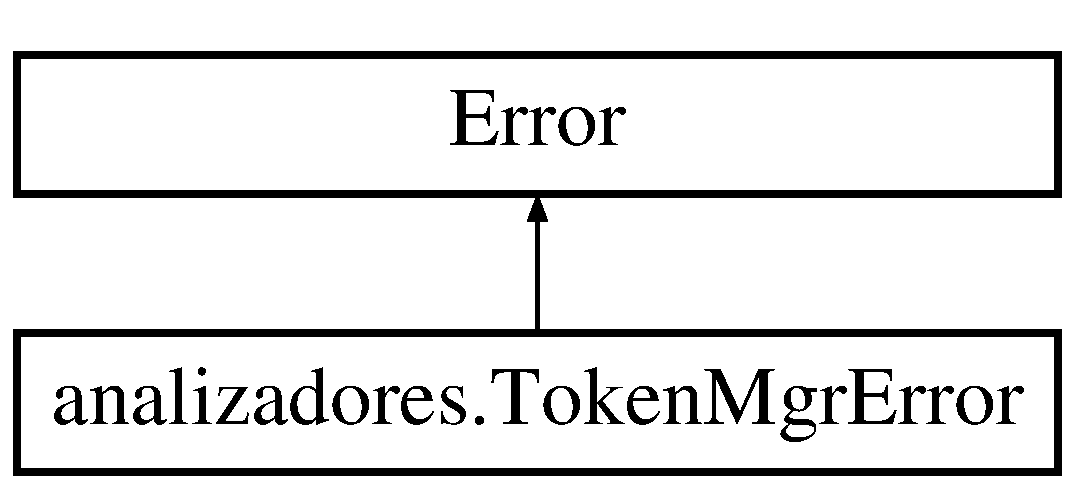
\includegraphics[height=2.000000cm]{classanalizadores_1_1_token_mgr_error}
\end{center}
\end{figure}
\subsection*{Public Member Functions}
\begin{DoxyCompactItemize}
\item 
String \mbox{\hyperlink{classanalizadores_1_1_token_mgr_error_a2ca09b102b2298a30e610bff62937adb}{get\+Message}} ()
\item 
\mbox{\hyperlink{classanalizadores_1_1_token_mgr_error_aae12e4756c58ebb1213e7793357fd5c6}{Token\+Mgr\+Error}} ()
\item 
\mbox{\hyperlink{classanalizadores_1_1_token_mgr_error_ac36479183b0a3b39cd4415c340dce78a}{Token\+Mgr\+Error}} (String message, int reason)
\item 
\mbox{\hyperlink{classanalizadores_1_1_token_mgr_error_a085945c54985dd2a5c5281088d055e67}{Token\+Mgr\+Error}} (boolean E\+O\+F\+Seen, int lex\+State, int error\+Line, int error\+Column, String error\+After, char cur\+Char, int reason)
\end{DoxyCompactItemize}
\subsection*{Static Protected Member Functions}
\begin{DoxyCompactItemize}
\item 
static final String \mbox{\hyperlink{classanalizadores_1_1_token_mgr_error_a4d339ae7110c798549b2c27c2317bc0a}{add\+Escapes}} (String str)
\item 
static String \mbox{\hyperlink{classanalizadores_1_1_token_mgr_error_a4d3448e37bf6a5bcff202bd569fe0410}{Lexical\+Error}} (boolean E\+O\+F\+Seen, int lex\+State, int error\+Line, int error\+Column, String error\+After, char cur\+Char)
\end{DoxyCompactItemize}


\subsection{Detailed Description}
\mbox{\hyperlink{classanalizadores_1_1_token}{Token}} Manager Error. 

\subsection{Constructor \& Destructor Documentation}
\mbox{\Hypertarget{classanalizadores_1_1_token_mgr_error_aae12e4756c58ebb1213e7793357fd5c6}\label{classanalizadores_1_1_token_mgr_error_aae12e4756c58ebb1213e7793357fd5c6}} 
\index{analizadores\+::\+Token\+Mgr\+Error@{analizadores\+::\+Token\+Mgr\+Error}!Token\+Mgr\+Error@{Token\+Mgr\+Error}}
\index{Token\+Mgr\+Error@{Token\+Mgr\+Error}!analizadores\+::\+Token\+Mgr\+Error@{analizadores\+::\+Token\+Mgr\+Error}}
\subsubsection{\texorpdfstring{Token\+Mgr\+Error()}{TokenMgrError()}\hspace{0.1cm}{\footnotesize\ttfamily [1/3]}}
{\footnotesize\ttfamily analizadores.\+Token\+Mgr\+Error.\+Token\+Mgr\+Error (\begin{DoxyParamCaption}{ }\end{DoxyParamCaption})}

No arg constructor. \mbox{\Hypertarget{classanalizadores_1_1_token_mgr_error_ac36479183b0a3b39cd4415c340dce78a}\label{classanalizadores_1_1_token_mgr_error_ac36479183b0a3b39cd4415c340dce78a}} 
\index{analizadores\+::\+Token\+Mgr\+Error@{analizadores\+::\+Token\+Mgr\+Error}!Token\+Mgr\+Error@{Token\+Mgr\+Error}}
\index{Token\+Mgr\+Error@{Token\+Mgr\+Error}!analizadores\+::\+Token\+Mgr\+Error@{analizadores\+::\+Token\+Mgr\+Error}}
\subsubsection{\texorpdfstring{Token\+Mgr\+Error()}{TokenMgrError()}\hspace{0.1cm}{\footnotesize\ttfamily [2/3]}}
{\footnotesize\ttfamily analizadores.\+Token\+Mgr\+Error.\+Token\+Mgr\+Error (\begin{DoxyParamCaption}\item[{String}]{message,  }\item[{int}]{reason }\end{DoxyParamCaption})}

Constructor with message and reason. \mbox{\Hypertarget{classanalizadores_1_1_token_mgr_error_a085945c54985dd2a5c5281088d055e67}\label{classanalizadores_1_1_token_mgr_error_a085945c54985dd2a5c5281088d055e67}} 
\index{analizadores\+::\+Token\+Mgr\+Error@{analizadores\+::\+Token\+Mgr\+Error}!Token\+Mgr\+Error@{Token\+Mgr\+Error}}
\index{Token\+Mgr\+Error@{Token\+Mgr\+Error}!analizadores\+::\+Token\+Mgr\+Error@{analizadores\+::\+Token\+Mgr\+Error}}
\subsubsection{\texorpdfstring{Token\+Mgr\+Error()}{TokenMgrError()}\hspace{0.1cm}{\footnotesize\ttfamily [3/3]}}
{\footnotesize\ttfamily analizadores.\+Token\+Mgr\+Error.\+Token\+Mgr\+Error (\begin{DoxyParamCaption}\item[{boolean}]{E\+O\+F\+Seen,  }\item[{int}]{lex\+State,  }\item[{int}]{error\+Line,  }\item[{int}]{error\+Column,  }\item[{String}]{error\+After,  }\item[{char}]{cur\+Char,  }\item[{int}]{reason }\end{DoxyParamCaption})}

Full Constructor. 

\subsection{Member Function Documentation}
\mbox{\Hypertarget{classanalizadores_1_1_token_mgr_error_a4d339ae7110c798549b2c27c2317bc0a}\label{classanalizadores_1_1_token_mgr_error_a4d339ae7110c798549b2c27c2317bc0a}} 
\index{analizadores\+::\+Token\+Mgr\+Error@{analizadores\+::\+Token\+Mgr\+Error}!add\+Escapes@{add\+Escapes}}
\index{add\+Escapes@{add\+Escapes}!analizadores\+::\+Token\+Mgr\+Error@{analizadores\+::\+Token\+Mgr\+Error}}
\subsubsection{\texorpdfstring{add\+Escapes()}{addEscapes()}}
{\footnotesize\ttfamily static final String analizadores.\+Token\+Mgr\+Error.\+add\+Escapes (\begin{DoxyParamCaption}\item[{String}]{str }\end{DoxyParamCaption})\hspace{0.3cm}{\ttfamily [static]}, {\ttfamily [protected]}}

Replaces unprintable characters by their escaped (or unicode escaped) equivalents in the given string \mbox{\Hypertarget{classanalizadores_1_1_token_mgr_error_a2ca09b102b2298a30e610bff62937adb}\label{classanalizadores_1_1_token_mgr_error_a2ca09b102b2298a30e610bff62937adb}} 
\index{analizadores\+::\+Token\+Mgr\+Error@{analizadores\+::\+Token\+Mgr\+Error}!get\+Message@{get\+Message}}
\index{get\+Message@{get\+Message}!analizadores\+::\+Token\+Mgr\+Error@{analizadores\+::\+Token\+Mgr\+Error}}
\subsubsection{\texorpdfstring{get\+Message()}{getMessage()}}
{\footnotesize\ttfamily String analizadores.\+Token\+Mgr\+Error.\+get\+Message (\begin{DoxyParamCaption}{ }\end{DoxyParamCaption})}

You can also modify the body of this method to customize your error messages. For example, cases like L\+O\+O\+P\+\_\+\+D\+E\+T\+E\+C\+T\+ED and I\+N\+V\+A\+L\+I\+D\+\_\+\+L\+E\+X\+I\+C\+A\+L\+\_\+\+S\+T\+A\+TE are not of end-\/users concern, so you can return something like \+: \begin{DoxyVerb}"Internal Error : Please file a bug report .... "
\end{DoxyVerb}


from this method for such cases in the release version of your parser. \mbox{\Hypertarget{classanalizadores_1_1_token_mgr_error_a4d3448e37bf6a5bcff202bd569fe0410}\label{classanalizadores_1_1_token_mgr_error_a4d3448e37bf6a5bcff202bd569fe0410}} 
\index{analizadores\+::\+Token\+Mgr\+Error@{analizadores\+::\+Token\+Mgr\+Error}!Lexical\+Error@{Lexical\+Error}}
\index{Lexical\+Error@{Lexical\+Error}!analizadores\+::\+Token\+Mgr\+Error@{analizadores\+::\+Token\+Mgr\+Error}}
\subsubsection{\texorpdfstring{Lexical\+Error()}{LexicalError()}}
{\footnotesize\ttfamily static String analizadores.\+Token\+Mgr\+Error.\+Lexical\+Error (\begin{DoxyParamCaption}\item[{boolean}]{E\+O\+F\+Seen,  }\item[{int}]{lex\+State,  }\item[{int}]{error\+Line,  }\item[{int}]{error\+Column,  }\item[{String}]{error\+After,  }\item[{char}]{cur\+Char }\end{DoxyParamCaption})\hspace{0.3cm}{\ttfamily [static]}, {\ttfamily [protected]}}

Returns a detailed message for the Error when it is thrown by the token manager to indicate a lexical error. Parameters \+: E\+O\+F\+Seen \+: indicates if E\+OF caused the lexical error cur\+Lex\+State \+: lexical state in which this error occurred error\+Line \+: line number when the error occurred error\+Column \+: column number when the error occurred error\+After \+: prefix that was seen before this error occurred curchar \+: the offending character Note\+: You can customize the lexical error message by modifying this method. 

The documentation for this class was generated from the following file\+:\begin{DoxyCompactItemize}
\item 
src/analizadores/Token\+Mgr\+Error.\+java\end{DoxyCompactItemize}

\hypertarget{classast_1_1instrucciones_1_1funciones_1_1_typeof}{}\section{ast.\+instrucciones.\+funciones.\+Typeof Class Reference}
\label{classast_1_1instrucciones_1_1funciones_1_1_typeof}\index{ast.\+instrucciones.\+funciones.\+Typeof@{ast.\+instrucciones.\+funciones.\+Typeof}}
Inheritance diagram for ast.\+instrucciones.\+funciones.\+Typeof\+:\begin{figure}[H]
\begin{center}
\leavevmode
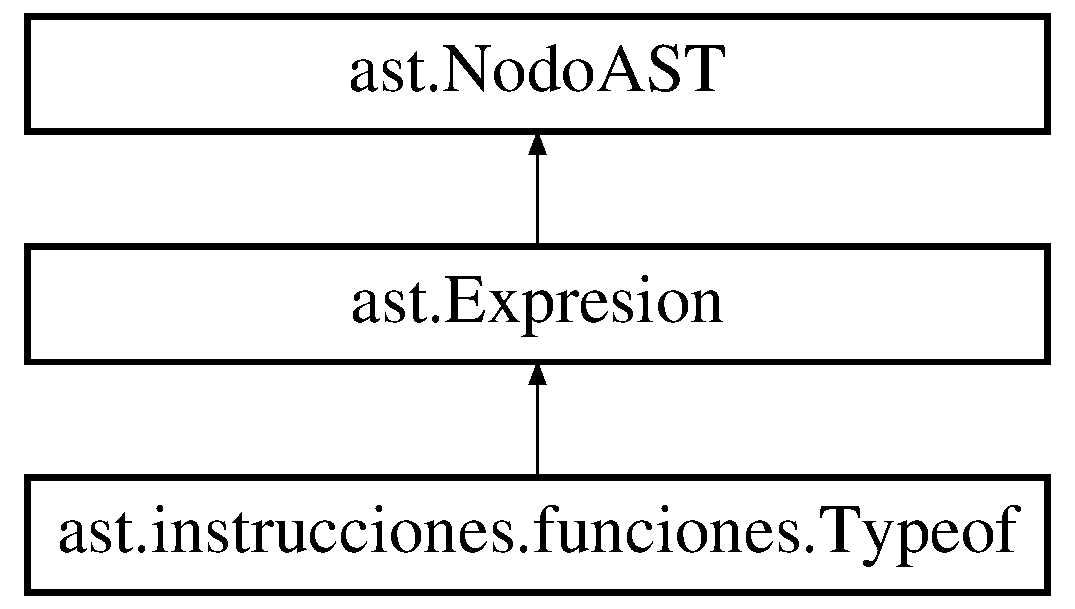
\includegraphics[height=3.000000cm]{classast_1_1instrucciones_1_1funciones_1_1_typeof}
\end{center}
\end{figure}
\subsection*{Public Member Functions}
\begin{DoxyCompactItemize}
\item 
\mbox{\Hypertarget{classast_1_1instrucciones_1_1funciones_1_1_typeof_a908895489aaf4127c246e59b36963a31}\label{classast_1_1instrucciones_1_1funciones_1_1_typeof_a908895489aaf4127c246e59b36963a31}} 
{\bfseries Typeof} (Linked\+List$<$ \mbox{\hyperlink{interfaceast_1_1_nodo_a_s_t}{Nodo\+A\+ST}} $>$ valor, int linea, int col)
\item 
\mbox{\Hypertarget{classast_1_1instrucciones_1_1funciones_1_1_typeof_ac15f6ad79e31e790ff634354a97ab7ba}\label{classast_1_1instrucciones_1_1funciones_1_1_typeof_ac15f6ad79e31e790ff634354a97ab7ba}} 
\mbox{\hyperlink{classentorno_1_1_tipo}{Tipo}} {\bfseries get\+Tipo} (\mbox{\hyperlink{classentorno_1_1_entorno}{Entorno}} ent)
\item 
\mbox{\Hypertarget{classast_1_1instrucciones_1_1funciones_1_1_typeof_a01492a71519eec4bc8b7e9c12a924023}\label{classast_1_1instrucciones_1_1funciones_1_1_typeof_a01492a71519eec4bc8b7e9c12a924023}} 
Object {\bfseries get\+Valor\+Implicito} (\mbox{\hyperlink{classentorno_1_1_entorno}{Entorno}} ent)
\item 
\mbox{\Hypertarget{classast_1_1instrucciones_1_1funciones_1_1_typeof_a5ade3fee74ef54aeebd5f9f698779776}\label{classast_1_1instrucciones_1_1funciones_1_1_typeof_a5ade3fee74ef54aeebd5f9f698779776}} 
int {\bfseries linea} ()
\item 
\mbox{\Hypertarget{classast_1_1instrucciones_1_1funciones_1_1_typeof_a87fe920f017636db6372097d9abd51fd}\label{classast_1_1instrucciones_1_1funciones_1_1_typeof_a87fe920f017636db6372097d9abd51fd}} 
int {\bfseries columna} ()
\item 
\mbox{\Hypertarget{classast_1_1instrucciones_1_1funciones_1_1_typeof_a7bb76411ad89a0bdce2083d197775fb5}\label{classast_1_1instrucciones_1_1funciones_1_1_typeof_a7bb76411ad89a0bdce2083d197775fb5}} 
String {\bfseries get\+Nombre} (String\+Builder builder, String parent, int cont)
\end{DoxyCompactItemize}


\subsection{Detailed Description}
\begin{DoxyAuthor}{Author}
p\+\_\+ab1 
\end{DoxyAuthor}


The documentation for this class was generated from the following file\+:\begin{DoxyCompactItemize}
\item 
src/ast/instrucciones/funciones/Typeof.\+java\end{DoxyCompactItemize}

\hypertarget{classentorno_1_1_var}{}\section{entorno.\+Var Class Reference}
\label{classentorno_1_1_var}\index{entorno.\+Var@{entorno.\+Var}}
\subsection*{Public Member Functions}
\begin{DoxyCompactItemize}
\item 
\mbox{\Hypertarget{classentorno_1_1_var_ae4d7c1cc982ac4e2477bdaba7b845f47}\label{classentorno_1_1_var_ae4d7c1cc982ac4e2477bdaba7b845f47}} 
{\bfseries Var} (String id, int dim)
\item 
\mbox{\Hypertarget{classentorno_1_1_var_a8d8494803f31d391b81ea9abe98f7189}\label{classentorno_1_1_var_a8d8494803f31d391b81ea9abe98f7189}} 
{\bfseries Var} (String id)
\item 
\mbox{\Hypertarget{classentorno_1_1_var_a429b876b41d8a7fbb63fddb683022f24}\label{classentorno_1_1_var_a429b876b41d8a7fbb63fddb683022f24}} 
String {\bfseries get\+Id} ()
\item 
\mbox{\Hypertarget{classentorno_1_1_var_ae720e983a433df23c17790caab117988}\label{classentorno_1_1_var_ae720e983a433df23c17790caab117988}} 
void {\bfseries set\+Id} (String id)
\item 
\mbox{\Hypertarget{classentorno_1_1_var_aa5d4e0d1740ed68f216594ea7380817b}\label{classentorno_1_1_var_aa5d4e0d1740ed68f216594ea7380817b}} 
int {\bfseries get\+Dim} ()
\item 
\mbox{\Hypertarget{classentorno_1_1_var_a975e7bb6df68b94aacd29986b88cd507}\label{classentorno_1_1_var_a975e7bb6df68b94aacd29986b88cd507}} 
void {\bfseries set\+Dim} (int dim)
\end{DoxyCompactItemize}


\subsection{Detailed Description}
\begin{DoxyAuthor}{Author}
p\+\_\+ab1 
\end{DoxyAuthor}


The documentation for this class was generated from the following file\+:\begin{DoxyCompactItemize}
\item 
src/entorno/Var.\+java\end{DoxyCompactItemize}

\hypertarget{classolc2_1_1p1__201504242_1_1_ventana}{}\section{olc2.\+p1\+\_\+201504242.\+Ventana Class Reference}
\label{classolc2_1_1p1__201504242_1_1_ventana}\index{olc2.\+p1\+\_\+201504242.\+Ventana@{olc2.\+p1\+\_\+201504242.\+Ventana}}
Inheritance diagram for olc2.\+p1\+\_\+201504242.\+Ventana\+:\begin{figure}[H]
\begin{center}
\leavevmode
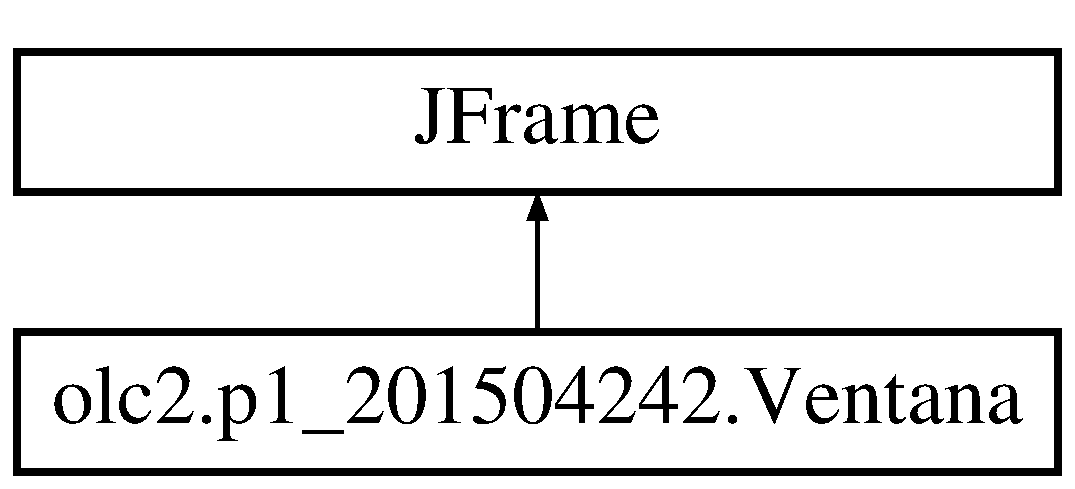
\includegraphics[height=2.000000cm]{classolc2_1_1p1__201504242_1_1_ventana}
\end{center}
\end{figure}
\subsection*{Public Member Functions}
\begin{DoxyCompactItemize}
\item 
\mbox{\hyperlink{classolc2_1_1p1__201504242_1_1_ventana_af29a17e75dff62d1fe1fe4727989b63a}{Ventana}} ()
\item 
\mbox{\Hypertarget{classolc2_1_1p1__201504242_1_1_ventana_a10616d9a5ee1a9a6d8c30025c77cf097}\label{classolc2_1_1p1__201504242_1_1_ventana_a10616d9a5ee1a9a6d8c30025c77cf097}} 
void {\bfseries agregar\+Label} (String cad)
\item 
\mbox{\Hypertarget{classolc2_1_1p1__201504242_1_1_ventana_a3a50772014c6d0f0af4a17225b8be4dd}\label{classolc2_1_1p1__201504242_1_1_ventana_a3a50772014c6d0f0af4a17225b8be4dd}} 
void {\bfseries agregar\+Consola} (String cad)
\item 
\mbox{\Hypertarget{classolc2_1_1p1__201504242_1_1_ventana_a13bbd13ef2ef35ddf0f58084bf603dd0}\label{classolc2_1_1p1__201504242_1_1_ventana_a13bbd13ef2ef35ddf0f58084bf603dd0}} 
void {\bfseries limpiar} ()
\end{DoxyCompactItemize}
\subsection*{Static Public Member Functions}
\begin{DoxyCompactItemize}
\item 
\mbox{\Hypertarget{classolc2_1_1p1__201504242_1_1_ventana_a3281e96c7bc31ff8986f9e4ee858672d}\label{classolc2_1_1p1__201504242_1_1_ventana_a3281e96c7bc31ff8986f9e4ee858672d}} 
static \mbox{\hyperlink{classolc2_1_1p1__201504242_1_1_ventana}{Ventana}} {\bfseries gget\+Ventana} ()
\item 
static void \mbox{\hyperlink{classolc2_1_1p1__201504242_1_1_ventana_a8ec2c001f5d8f7f18fd9da6429e0e3c0}{main}} (String args\mbox{[}$\,$\mbox{]})
\end{DoxyCompactItemize}
\subsection*{Public Attributes}
\begin{DoxyCompactItemize}
\item 
\mbox{\Hypertarget{classolc2_1_1p1__201504242_1_1_ventana_a2c943cc0666abd75d572f7cceb873e9c}\label{classolc2_1_1p1__201504242_1_1_ventana_a2c943cc0666abd75d572f7cceb873e9c}} 
Linked\+List$<$ \mbox{\hyperlink{classolc2_1_1p1__201504242_1_1_j_error}{J\+Error}} $>$ {\bfseries lista\+Error} = new Linked\+List()
\end{DoxyCompactItemize}


\subsection{Detailed Description}
\begin{DoxyAuthor}{Author}
p\+\_\+ab1 
\end{DoxyAuthor}


\subsection{Constructor \& Destructor Documentation}
\mbox{\Hypertarget{classolc2_1_1p1__201504242_1_1_ventana_af29a17e75dff62d1fe1fe4727989b63a}\label{classolc2_1_1p1__201504242_1_1_ventana_af29a17e75dff62d1fe1fe4727989b63a}} 
\index{olc2\+::p1\+\_\+201504242\+::\+Ventana@{olc2\+::p1\+\_\+201504242\+::\+Ventana}!Ventana@{Ventana}}
\index{Ventana@{Ventana}!olc2\+::p1\+\_\+201504242\+::\+Ventana@{olc2\+::p1\+\_\+201504242\+::\+Ventana}}
\subsubsection{\texorpdfstring{Ventana()}{Ventana()}}
{\footnotesize\ttfamily olc2.\+p1\+\_\+201504242.\+Ventana.\+Ventana (\begin{DoxyParamCaption}{ }\end{DoxyParamCaption})}

Creates new form \mbox{\hyperlink{classolc2_1_1p1__201504242_1_1_ventana}{Ventana}} 

\subsection{Member Function Documentation}
\mbox{\Hypertarget{classolc2_1_1p1__201504242_1_1_ventana_a8ec2c001f5d8f7f18fd9da6429e0e3c0}\label{classolc2_1_1p1__201504242_1_1_ventana_a8ec2c001f5d8f7f18fd9da6429e0e3c0}} 
\index{olc2\+::p1\+\_\+201504242\+::\+Ventana@{olc2\+::p1\+\_\+201504242\+::\+Ventana}!main@{main}}
\index{main@{main}!olc2\+::p1\+\_\+201504242\+::\+Ventana@{olc2\+::p1\+\_\+201504242\+::\+Ventana}}
\subsubsection{\texorpdfstring{main()}{main()}}
{\footnotesize\ttfamily static void olc2.\+p1\+\_\+201504242.\+Ventana.\+main (\begin{DoxyParamCaption}\item[{String}]{args\mbox{[}$\,$\mbox{]} }\end{DoxyParamCaption})\hspace{0.3cm}{\ttfamily [static]}}


\begin{DoxyParams}{Parameters}
{\em args} & the command line arguments \\
\hline
\end{DoxyParams}


The documentation for this class was generated from the following file\+:\begin{DoxyCompactItemize}
\item 
src/olc2/p1\+\_\+201504242/Ventana.\+java\end{DoxyCompactItemize}

\hypertarget{classast_1_1instrucciones_1_1_while}{}\section{ast.\+instrucciones.\+While Class Reference}
\label{classast_1_1instrucciones_1_1_while}\index{ast.\+instrucciones.\+While@{ast.\+instrucciones.\+While}}
Inheritance diagram for ast.\+instrucciones.\+While\+:\begin{figure}[H]
\begin{center}
\leavevmode
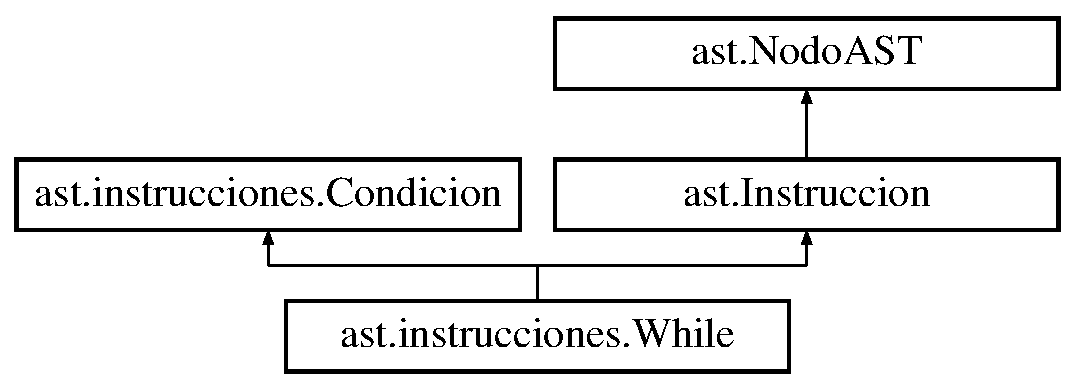
\includegraphics[height=3.000000cm]{classast_1_1instrucciones_1_1_while}
\end{center}
\end{figure}
\subsection*{Public Member Functions}
\begin{DoxyCompactItemize}
\item 
\mbox{\Hypertarget{classast_1_1instrucciones_1_1_while_a03f3cb9d5fb7ab2f38f7a750074bd183}\label{classast_1_1instrucciones_1_1_while_a03f3cb9d5fb7ab2f38f7a750074bd183}} 
{\bfseries While} (Linked\+List$<$ \mbox{\hyperlink{interfaceast_1_1_nodo_a_s_t}{Nodo\+A\+ST}} $>$ ins, \mbox{\hyperlink{interfaceast_1_1_expresion}{Expresion}} cond, int linea, int col)
\item 
\mbox{\Hypertarget{classast_1_1instrucciones_1_1_while_a26e0e7c8a6013fb5898da8ed6a796cf8}\label{classast_1_1instrucciones_1_1_while_a26e0e7c8a6013fb5898da8ed6a796cf8}} 
Object {\bfseries ejecutar} (\mbox{\hyperlink{classentorno_1_1_entorno}{Entorno}} ent)
\item 
\mbox{\Hypertarget{classast_1_1instrucciones_1_1_while_a6e965ceedcfaf83d93996b284a8c98fc}\label{classast_1_1instrucciones_1_1_while_a6e965ceedcfaf83d93996b284a8c98fc}} 
int {\bfseries linea} ()
\item 
\mbox{\Hypertarget{classast_1_1instrucciones_1_1_while_ada9c390065cfd7a7e975b090b76ac400}\label{classast_1_1instrucciones_1_1_while_ada9c390065cfd7a7e975b090b76ac400}} 
int {\bfseries columna} ()
\item 
\mbox{\Hypertarget{classast_1_1instrucciones_1_1_while_a6b00b28f9737cdbffe6f413d33cdc951}\label{classast_1_1instrucciones_1_1_while_a6b00b28f9737cdbffe6f413d33cdc951}} 
String {\bfseries get\+Nombre} (String\+Builder builder, String parent, int cont)
\end{DoxyCompactItemize}


\subsection{Detailed Description}
\begin{DoxyAuthor}{Author}
p\+\_\+ab1 
\end{DoxyAuthor}


The documentation for this class was generated from the following file\+:\begin{DoxyCompactItemize}
\item 
src/ast/instrucciones/While.\+java\end{DoxyCompactItemize}

%--- End generated contents ---

% Index
\backmatter
\newpage
\phantomsection
\clearemptydoublepage
\addcontentsline{toc}{chapter}{Index}
\printindex

\end{document}
